\chapter{Przeprowadzone badania}
W niniejszym rozdziale przedstawiono oraz omówiono badania przeprowadzone w celu ewaluacji wydajności interfejsów API implementowanych z wykorzystaniem porównywanych technologii. Każde z wykonanych badań oparte jest o scenariusz testowy określony w ramach sekcji \ref{sec:scenariusze-badawcze}, a także dotyczy odmiennych aspektów działania usługi sieciowej interfejsu programowania aplikacji. W kojenych sekcjach tego rozdziału w sposób szczegółowy opisano podjęte czynności badawcze, zwizualizowano rezultaty każdej z ewaluacji, dokonano analizy statystycznej, a także sformułowano wnioski.

\section{Wpływ zastosowanego systemu bazodanowego na efektywność działania interfejsu API}
\label{research:crud}
W ramach badania zobserwowano zmianę wydajności działania interfejsów programowania aplikacji względem skomunikowanego z nim systemu bazodanowego. Wykorzystano cztery najpopularniejsze relacyjne systemy baz danych (tj. MySQL, SQL Sever, PostgreSQL oraz SQlite), a także jeden system nierelacyjny (tj. MongoDB). Interfejsy programowania aplikacji komunikujące się z poszczególnymi systemami bazodanowymi poddawane były coraz to większemu obciążeniu, poprzez zwiększanie liczby procesów generujących żądania.

Pierwszą czynnością wykonaną w ramach ewaluacji było spełnienie warunków początkowych dotyczących podjęcia czynności badawczych. Warunki te, uwzględniały realizację testów funkcjonalnych gwarantujących poprawność działania punktów końcowych interfejsu programowania aplikacji. Ponadto, przeprowadzenie tego rodzaju testów pozwoliło na określenie progów tolerancji oraz frustracji wykorzystywanych w kontekście późniejszego wyliczania wartości wskaźnika wydajności aplikacji APDEX.

Ewaluacja funkcjonalna, polegała na uruchomieniu testu uwzględniającego 30 współbieżnie pracujących wątków oprogramowania JMeter, które wysyłały żądania w kierunku punktów końcowych API w czasie 10 minut.

Poczynione zostały dwa następujące założenia:
\begin{itemize}
    \item generowanie żądań przez 30 współbieżnych procesów jest interpretowane jako funkcjonowanie interfejsu programowania aplikacji w standardowych warunkach pracy.
    \item ogólna ocena wydajności systemu, a także progi uwzględniane w ramach wskaźnika APDEX generowane są na podstawie tylko tych punktów końcowych, które poddawane są ewaluacji.
\end{itemize}

Zdecydowano się na wybór pięciu punktów końcowych obsługujących różne metody protokołu hipertekstowego, po to, aby weryfikować każdy rodzaj działania uwzględnianego w ramach funkcjonalności interfejsu API.

W tabeli \ref{tab:endpointy-scenario-1} wyszczególniono każdy z wykorzystywanych punktów końcowych interfejsów programowania aplikacji, a także opisano sposób jego działania.

\begin{table}[htb]
  \centering
  \caption{Wykaz punktów końcowych wykorzystywanych w badaniu wpływu wykorzystanego systemu bazodanowego na działanie API}
  \label{tab:endpointy-scenario-1}
  \resizebox{\columnwidth}{!}{%
  \begin{tabular}[c]{|l|m{0.4\textwidth}|l|m{0.4\textwidth}|}
  \hline
  Identyfikator zasobu &
    Dostarczana zawartość &
    \begin{tabular}[c]{@{}l@{}}Rodzaj \\ metody HTTP\end{tabular} &
    Opis działania \\ \hline\hline
  /api/bills &
    \begin{tabular}[c]{@{}l@{}}\textbf{pageSize} - rozmiar strony (tj. liczba \\ rekordów) -- ustalony na stałe jako 30 \\ \textbf{pageNumber} - numer strony \\ -- generowany zgodnie z jednostajnym \\ rozkładem prawdopodobieństwa\end{tabular} &
    GET &
    Zwrócenie listy encji identyfikujących rachunki wygenerowane w restauracji. Zarówno rozmiar strony, jak i liczba pomijanych rekordów zadane są jako parametr, a poszczególny element listy, zawiera zarówno dane encji podstawowej, jak i każdej z encji zależnych, powiązanych z nią kluczem obcym. \\ \hline
  /api/orders/:id &
    \textbf{id} - identyfikator zamówienia wskazujący każdorazowo zamówienie istniejące w bazie danych &
    GET &
    Zwrócenie pojedynczej encji identyfikującej określone zamówienie poczynione w ramach pobytu w restauracji. Zwrócony element zawiera zarówno dane encji podstawowej, jak i każdej z encji zależnych, powiązanych z nią kluczem obcym. \\ \hline
  /api/products &
  \textbf{saveProductBody} - zasób zapisany w formacie JSON, dostarczający informacje o wartościach właściwości nowo tworzonego produktu -- każdy z identyfikatorów encji zależnych wskazuje na istniejący obiekt &
    POST &
    Dodanie pojedynczej encji do zbioru danych z poprzedzającą je walidacją danych dostarczonych w ramach ciała żądania. \\ \hline
  /api/courses/:id &
  \begin{tabular}[c]{@{}l@{}} \textbf{id} - identyfikator posiłku zawartego \\ w ramach zamówienia wskazujący \\ każdorazowo istniejącą \\ encję bazodanową \\ updateCourseBody - zasób zapisany \\ w formacie JSON, dostarczający \\ informacje o wartościach właściwości \\ modyfikowanego obiektu posiłku \end{tabular} &
    PUT &
    Modyfikowanie encji bazodanowej dotyczącej posiłku zawartego w ramach zamówienia z uprzednią weryfikacją poprawności danych ciała żądania. \\ \hline
  /api/reservations/:id &
  \textbf{id} - identyfikator rezerwacji, wskazujący na istniejący bądź nieistniejący zasób &
    DELETE &
    Usunięcie pojedynczego obiektu rezerwacji, bądź zwrócenie informacji o jego nie znalezieniu w systemie bazodanowym. \\ \hline
  \end{tabular}%
  }
\end{table}

Na wykresie \ref{fig:wykres-testy-funkcjonalne-dotnet} przedstawiono rzeczywiste pomiary chwilowe czasu odpowiedzi na żądanie, uwzględniające rezultaty otrzymane dla każdego z omówionych punktów końcowych. Jako interfejs programowania aplikacji poddawany ewaluacji zastosowano usługę sieciową implementowaną w technologii C\#/.NET, a także komunikującą się z bazą danych SQL Server.

W ramach ewaluacji funkcjonalnej wszystkie wywołania badanych punktów końcowych zwróciły zarówno poprawny kod odpowiedzi, jak i spodziewaną zawartość. Obserwacja ta, pozwoliła na kontynuację badania oraz spełnienie jego warunków początkowych. 

\clearpage

\begin{figure}[htb]
    \centering
     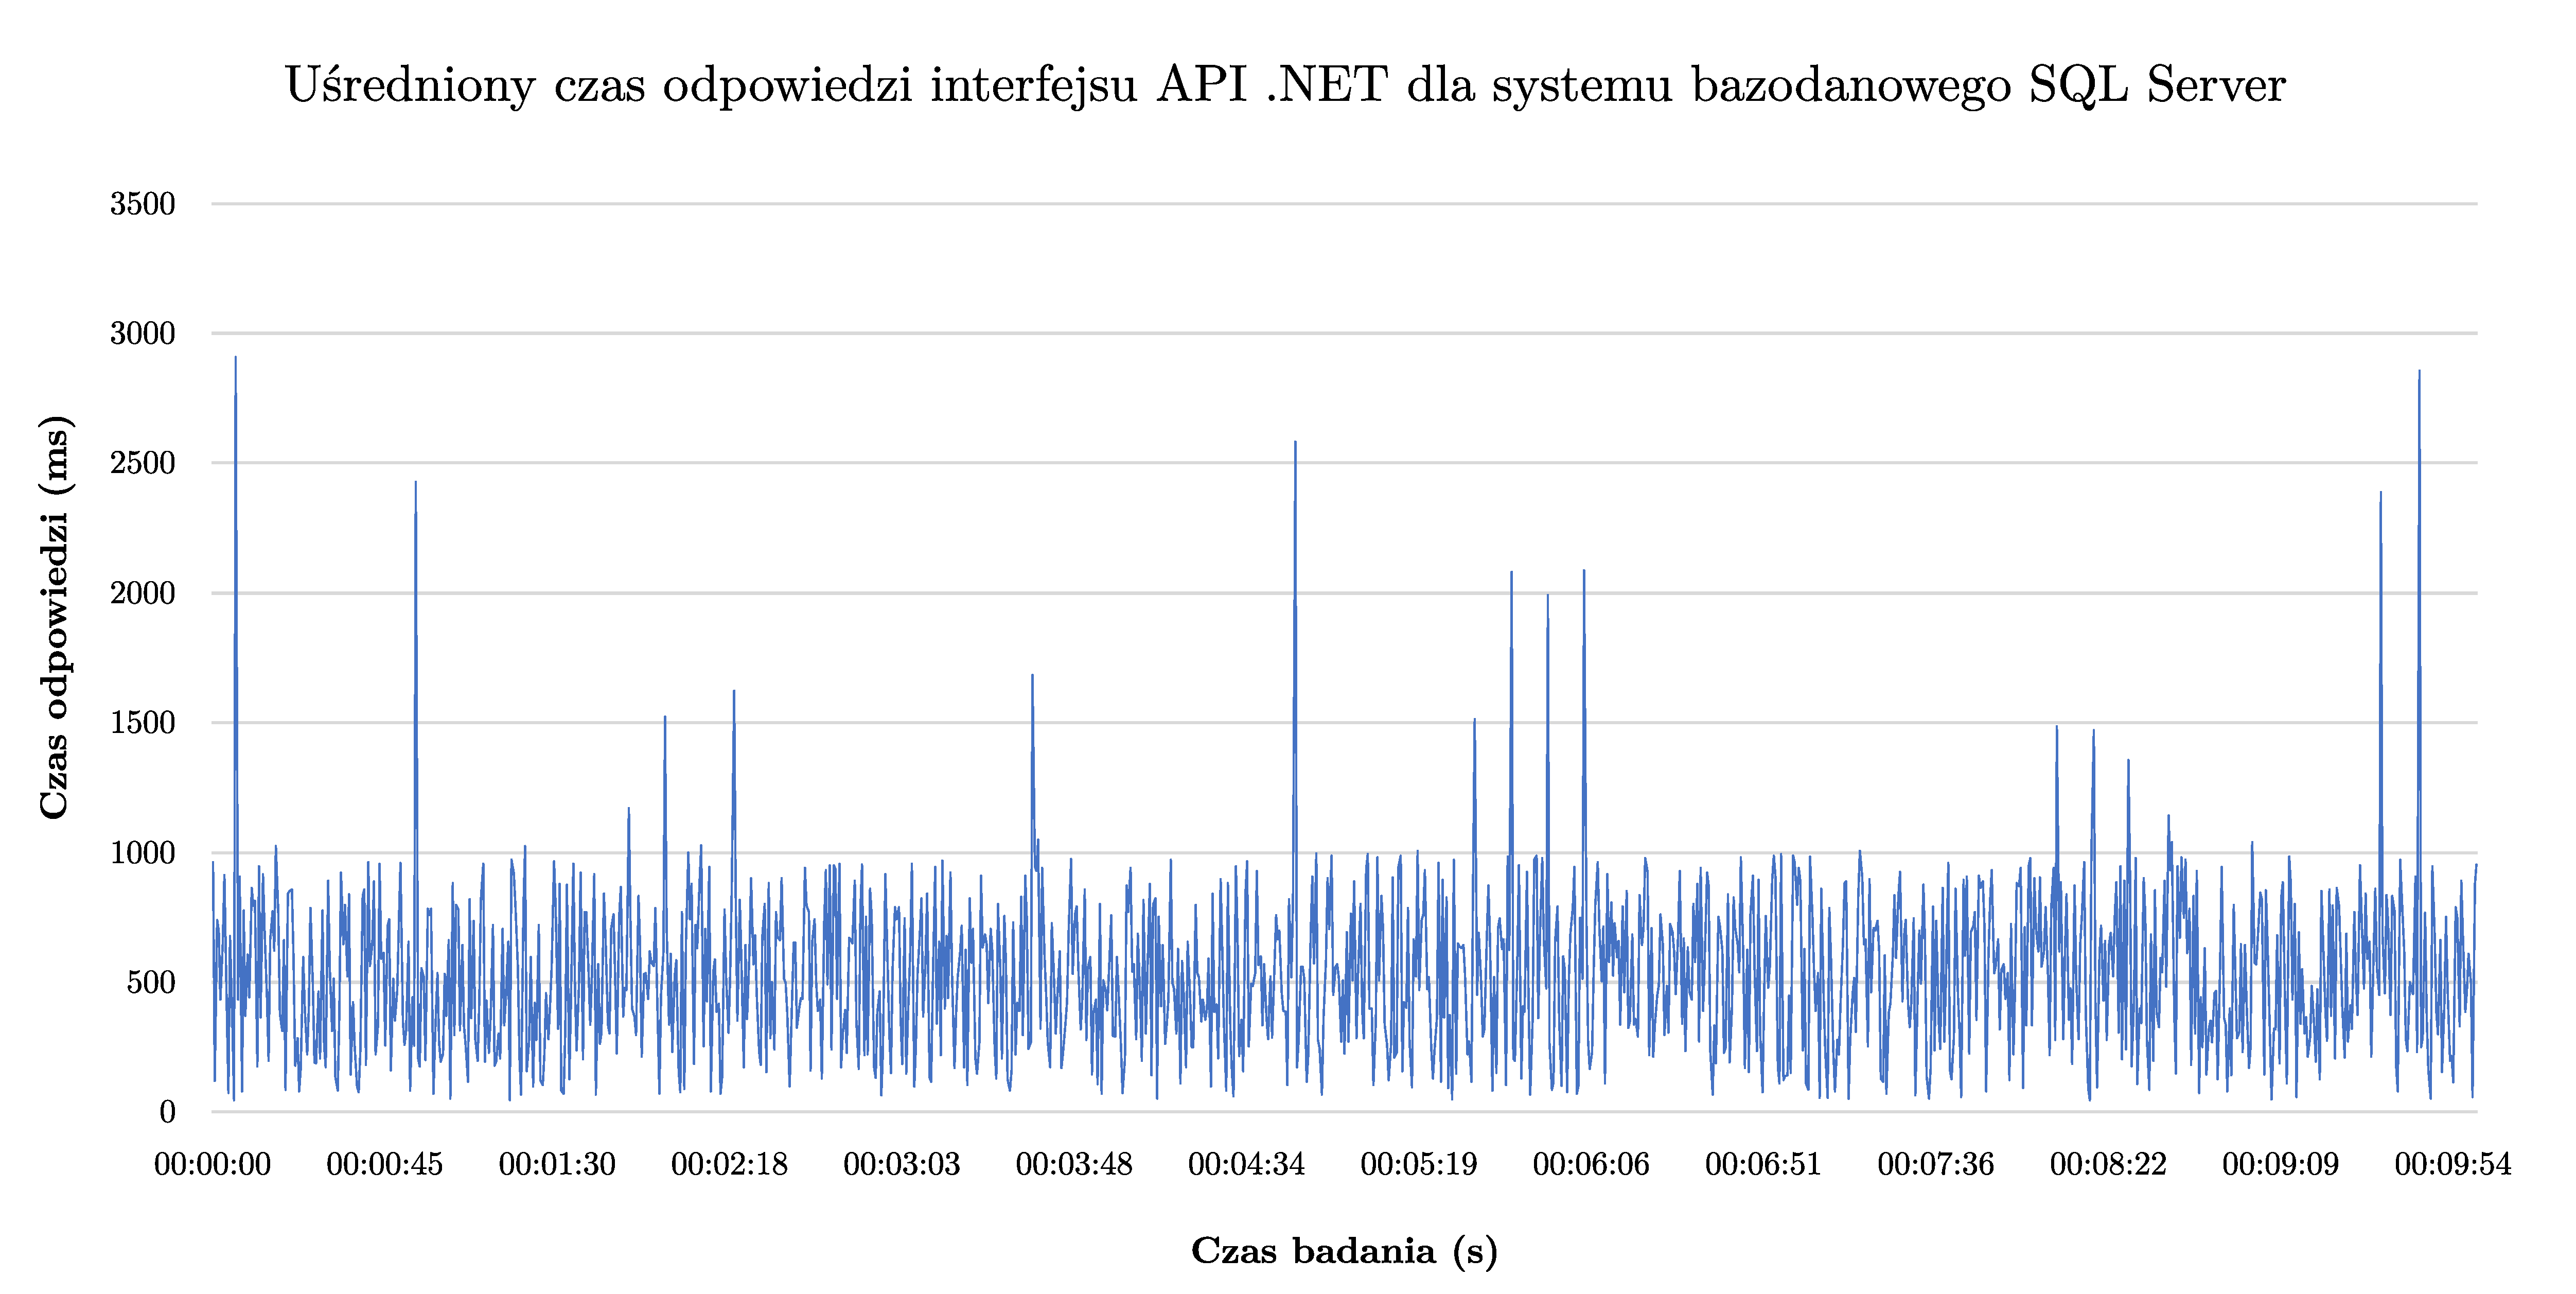
\includegraphics[width=\linewidth]{rys05/testy-funkcjonalne-dotnet.pdf}
    \caption{Rzeczywisty pomiar chwilowy czasu odpowiedzi na żądanie dla konfiguracji .NET/SQL Server w kontekście testu funkcjonalnego}
    \label{fig:wykres-testy-funkcjonalne-dotnet}
\end{figure}

Na podstawie analogicznych danych, dla każdej pary interfejs API -- system bazodanowy, zdefiniowano progi tolerancji oraz frustracji stanowiące punkty odniesienia przy kalkulacji wartości wskaźnika APDEX. Wartości te, ustalono poprzez rosnące posortowanie zbioru czasów odpowiedzi API, a następnie dokonanie symetrycznego podziału dwupunktowego.

Uzyskane przedziały satysfakcji, tolerancji oraz frustracji względem każdego systemu bazodanowego oraz technologii tworzenia API zostały zobrazowane na wykresach \ref{fig:apdex-dotnet} oraz \ref{fig:apdex-nodejs}.

\begin{figure}[htb]
    \centering
     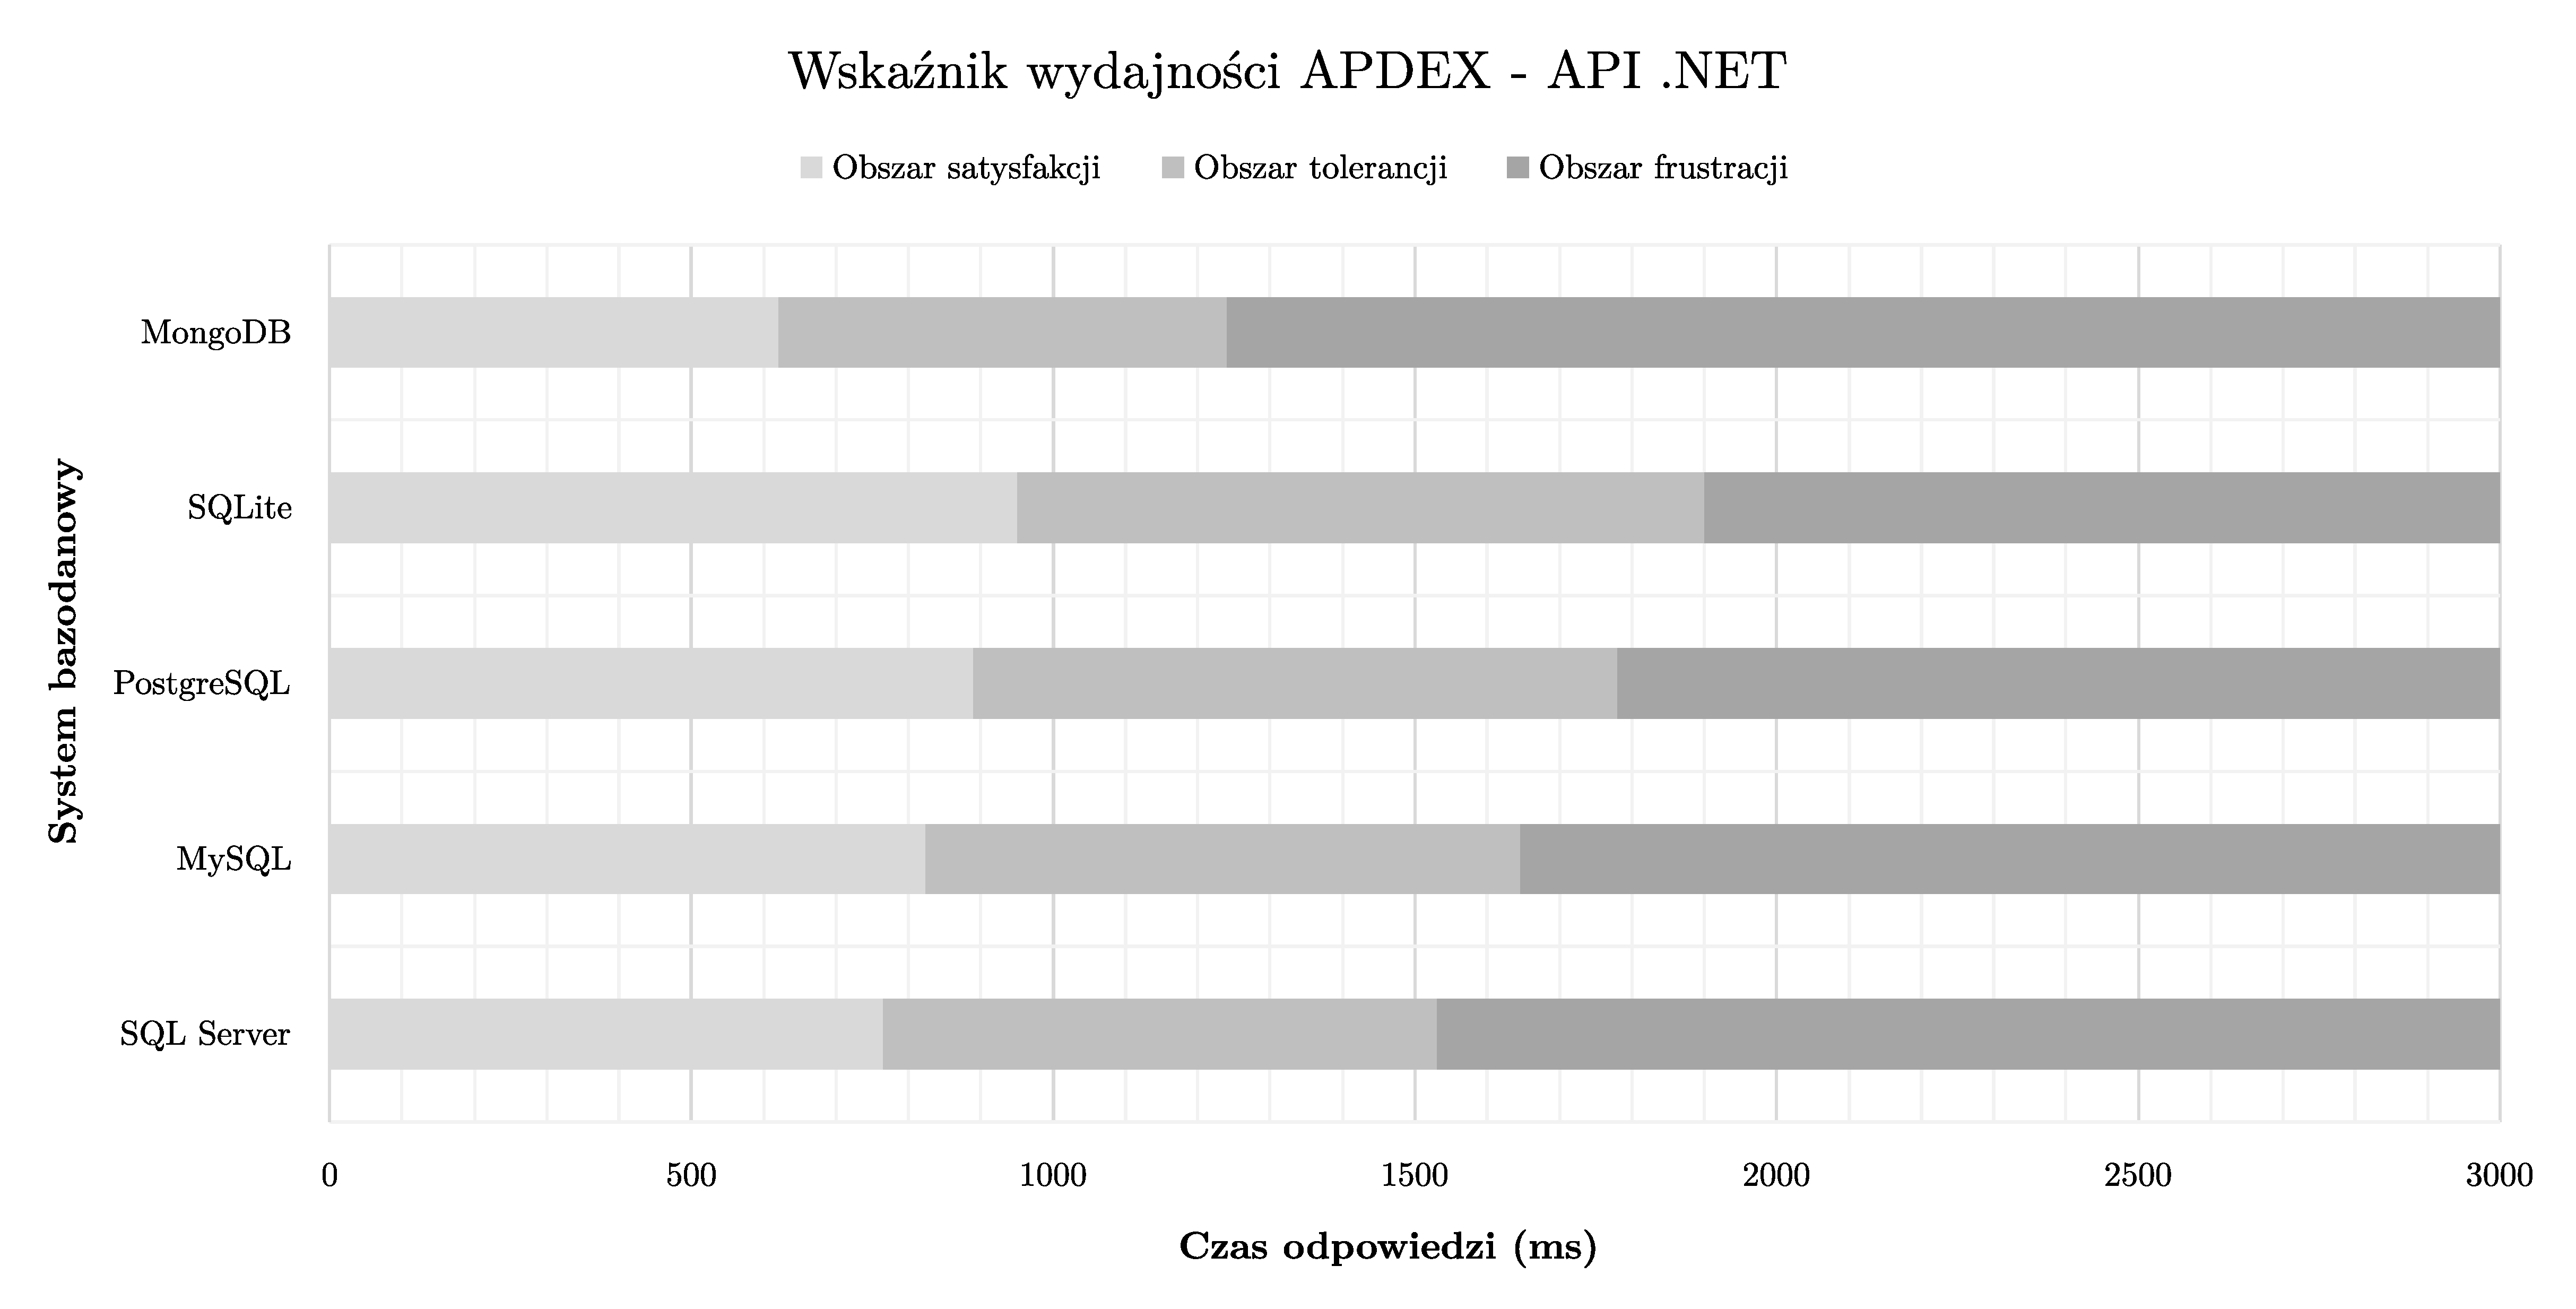
\includegraphics[width=\linewidth]{rys05/apdex-dotnet.pdf}
    \caption{Obszary satysfakcji, tolerancji oraz frustracji wskaźnika APDEX względem poszczególnych systemów bazodanowych dla API zaimplementowanego w C\#}
    \label{fig:apdex-dotnet}
\end{figure}

\clearpage

\begin{figure}[htb]
    \centering
     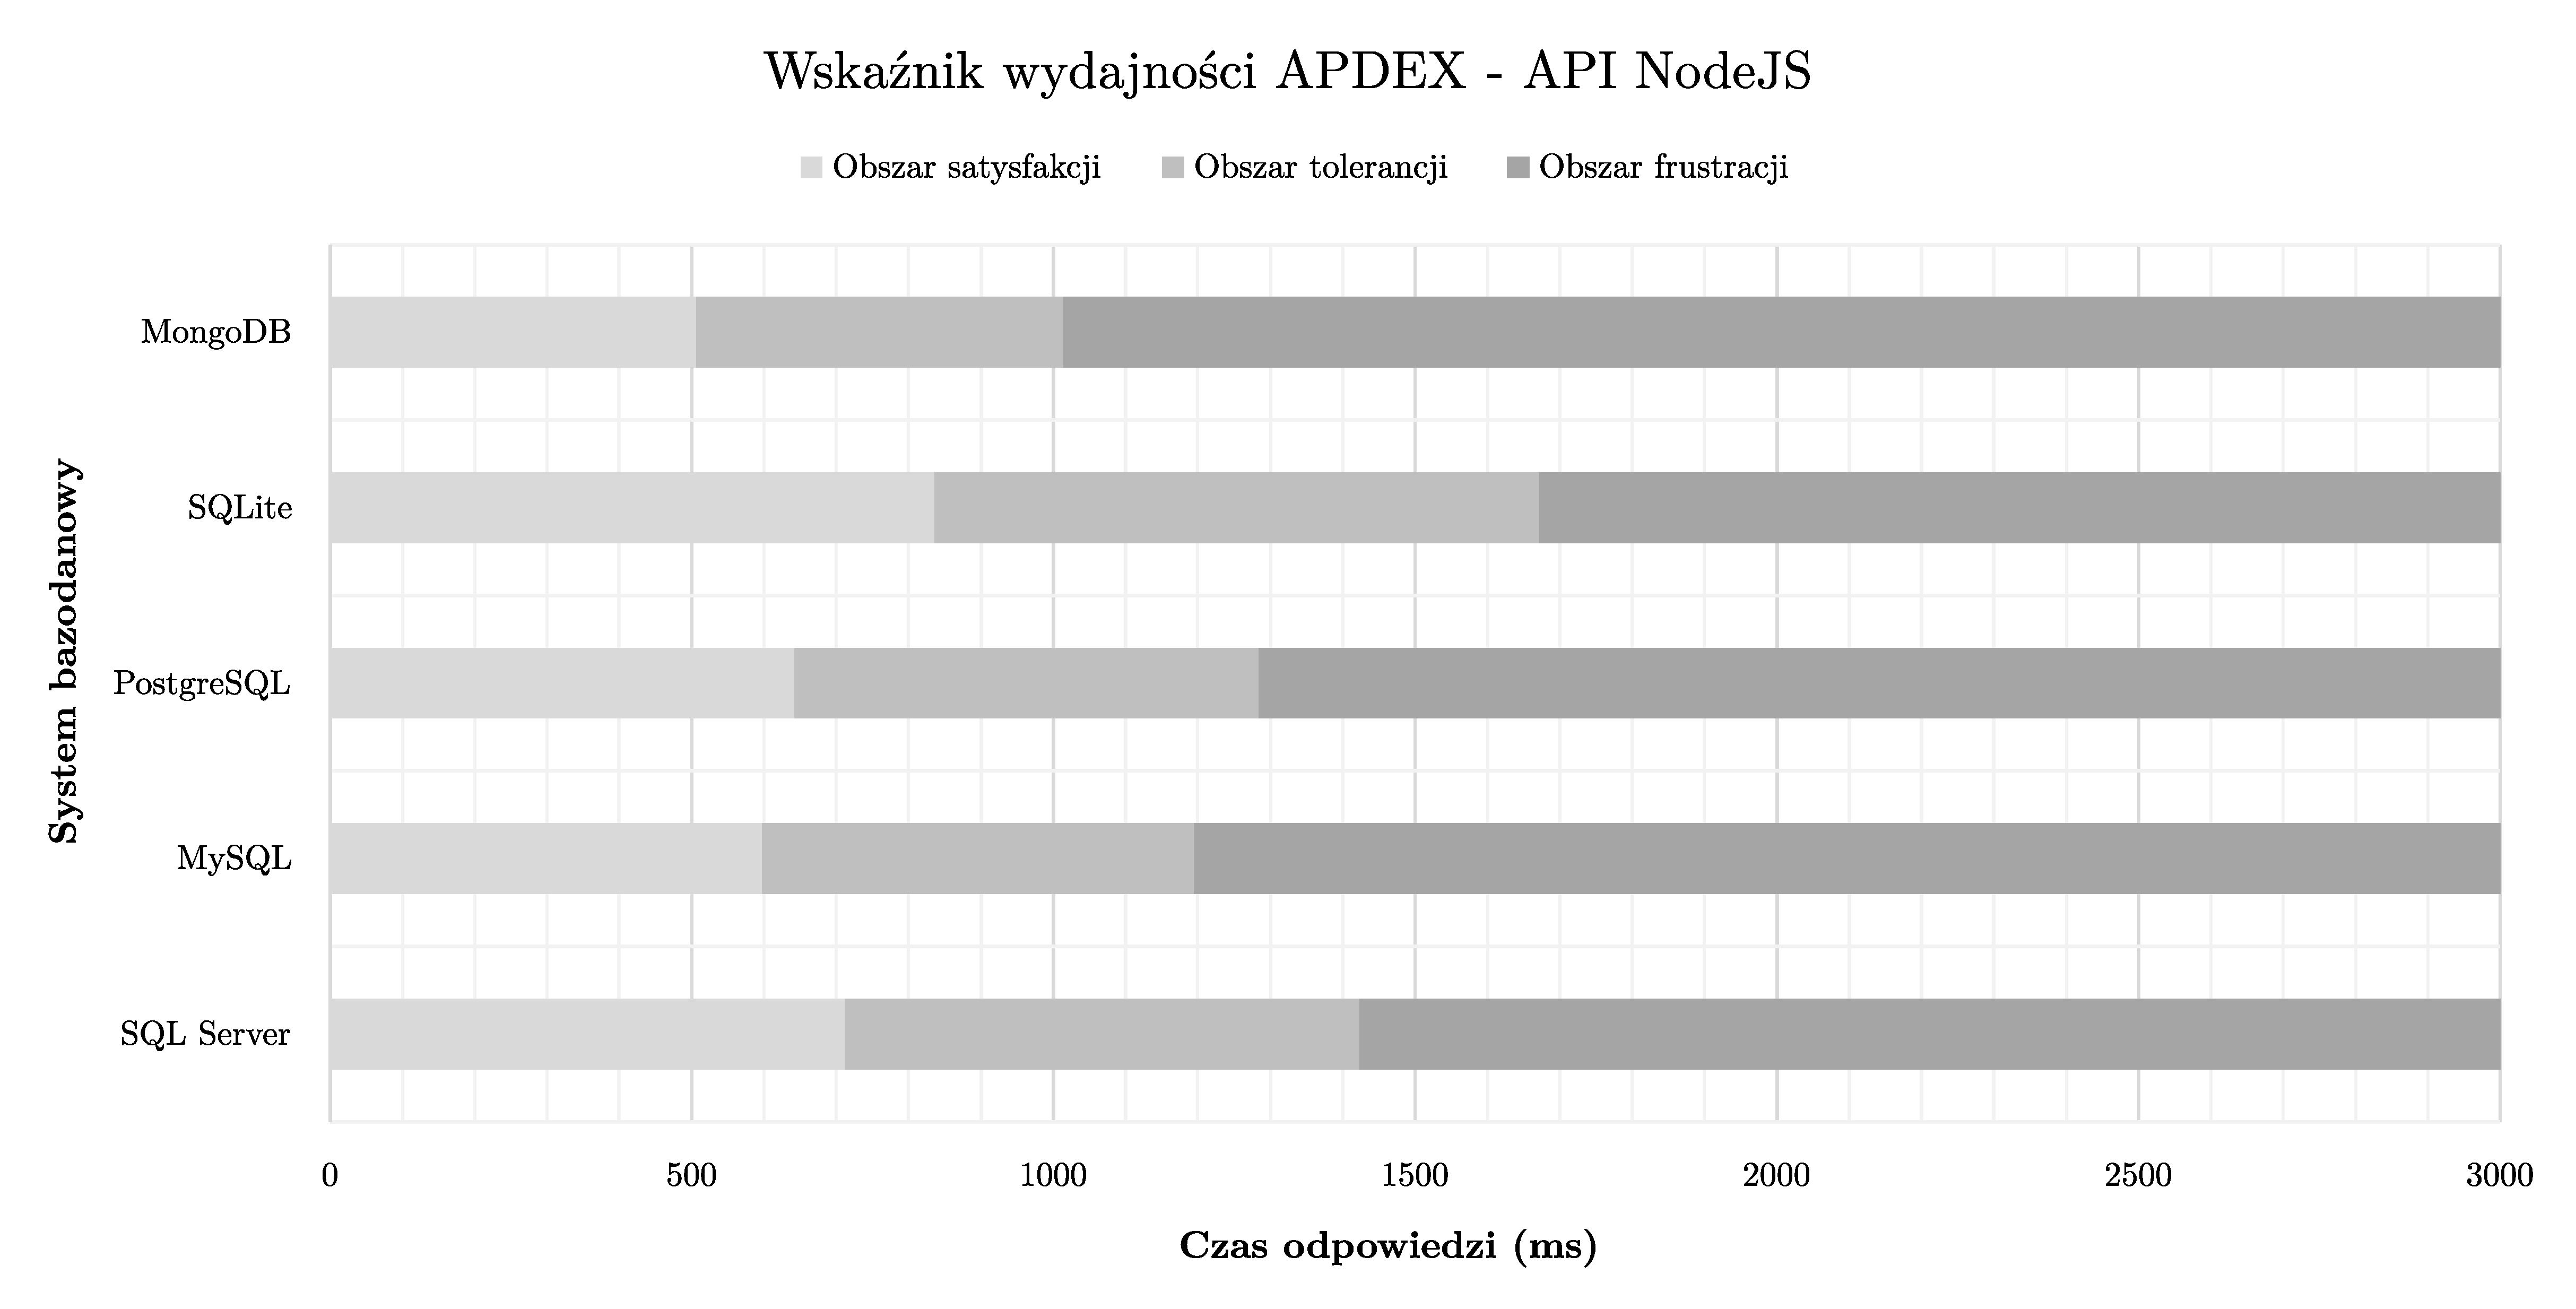
\includegraphics[width=\linewidth]{rys05/apdex-nodejs.pdf}
    \caption{Obszary satysfakcji, tolerancji oraz frustracji wskaźnika APDEX względem poszczególnych systemów bazodanowych dla API zaimplementowanego w JavaScript}
    \label{fig:apdex-nodejs}
\end{figure}

Po spełnieniu warunków początkowych badania zrealizowano faktyczne czynności badawcze. Wykorzystując lokalną topologię fizyczną nr 1, omówioną w ramach sekcji \ref{sec:lokalne-srodowisko-badawcze-ver-1} rozpoczęto generowanie żądań protokołu hipertekstowego wytwarzanych przez dwa równolegle pracujące hosty sieciowe. Procedura badawcza trwała 20 minut i polegała na stopniowym zwiększaniu liczby współbieżnie pracujących procesów oprogramowania testującego rozpoczynając od jednego procesu a kończąc na pięciu tysiącach. Nowe wątki oprogramowania Apache JMeter uruchamiane były w stałych odstępach czasu, co implikuje niezmienność długości przedziału czasowego pracy w obrębie ustalonej liczby wątków. Czas ten, wynosi 240 ms. Przy uwzględnieniu minimalnej zaobserwowanej średniej wartości natężenia generowanych żądań, wynoszącej 152 zapytania w ciągu sekundy, liczebność zbioru próbek czasu zapytania w odniesieniu do dowolnego z 4990 poziomów przyrostu ruchu wyniosła co najmniej 36 elementów. Pierwsze 10 poziomów dotyczących liczby klientów generujących komunikaty nie pozwoliło na zarejestrowanie co najmniej 30 próbek, przez co elementy te, nie były brane pod uwagę w czasie opracowywania uzyskanych wyników. Opisane w niniejszym akapicie czynności zostały wykonane względem interfejsów programowania aplikacji wykorzystujących porównywane technologie, uwzględniając komunikację z każdym z pięciu systemów bazodanowych.

Na wykresach \ref{fig:response-mtc-1} a) do \ref{fig:response-mtc-1} j) zaprezentowano uśrednione względem liczby pracujących wątków, czasy odpowiedzi na żądanie generowane w kierunku ewaluowanych interfejsów API.

Analizując wyniki uzyskane dla operacji pobierania kolekcji obiektów, zauważyć można niewielkie różnice w wartości średnich czasów odpowiedzi, występujące w przedziale do około 4000 użytkowników. Różnice te, nie faworyzują ani deprecjonują któregokolwiek z rozwiązań.

\begin{figure}[H]
  \centering
	\begin{tabular}{@{}ll@{}}
    a) & b) \\
    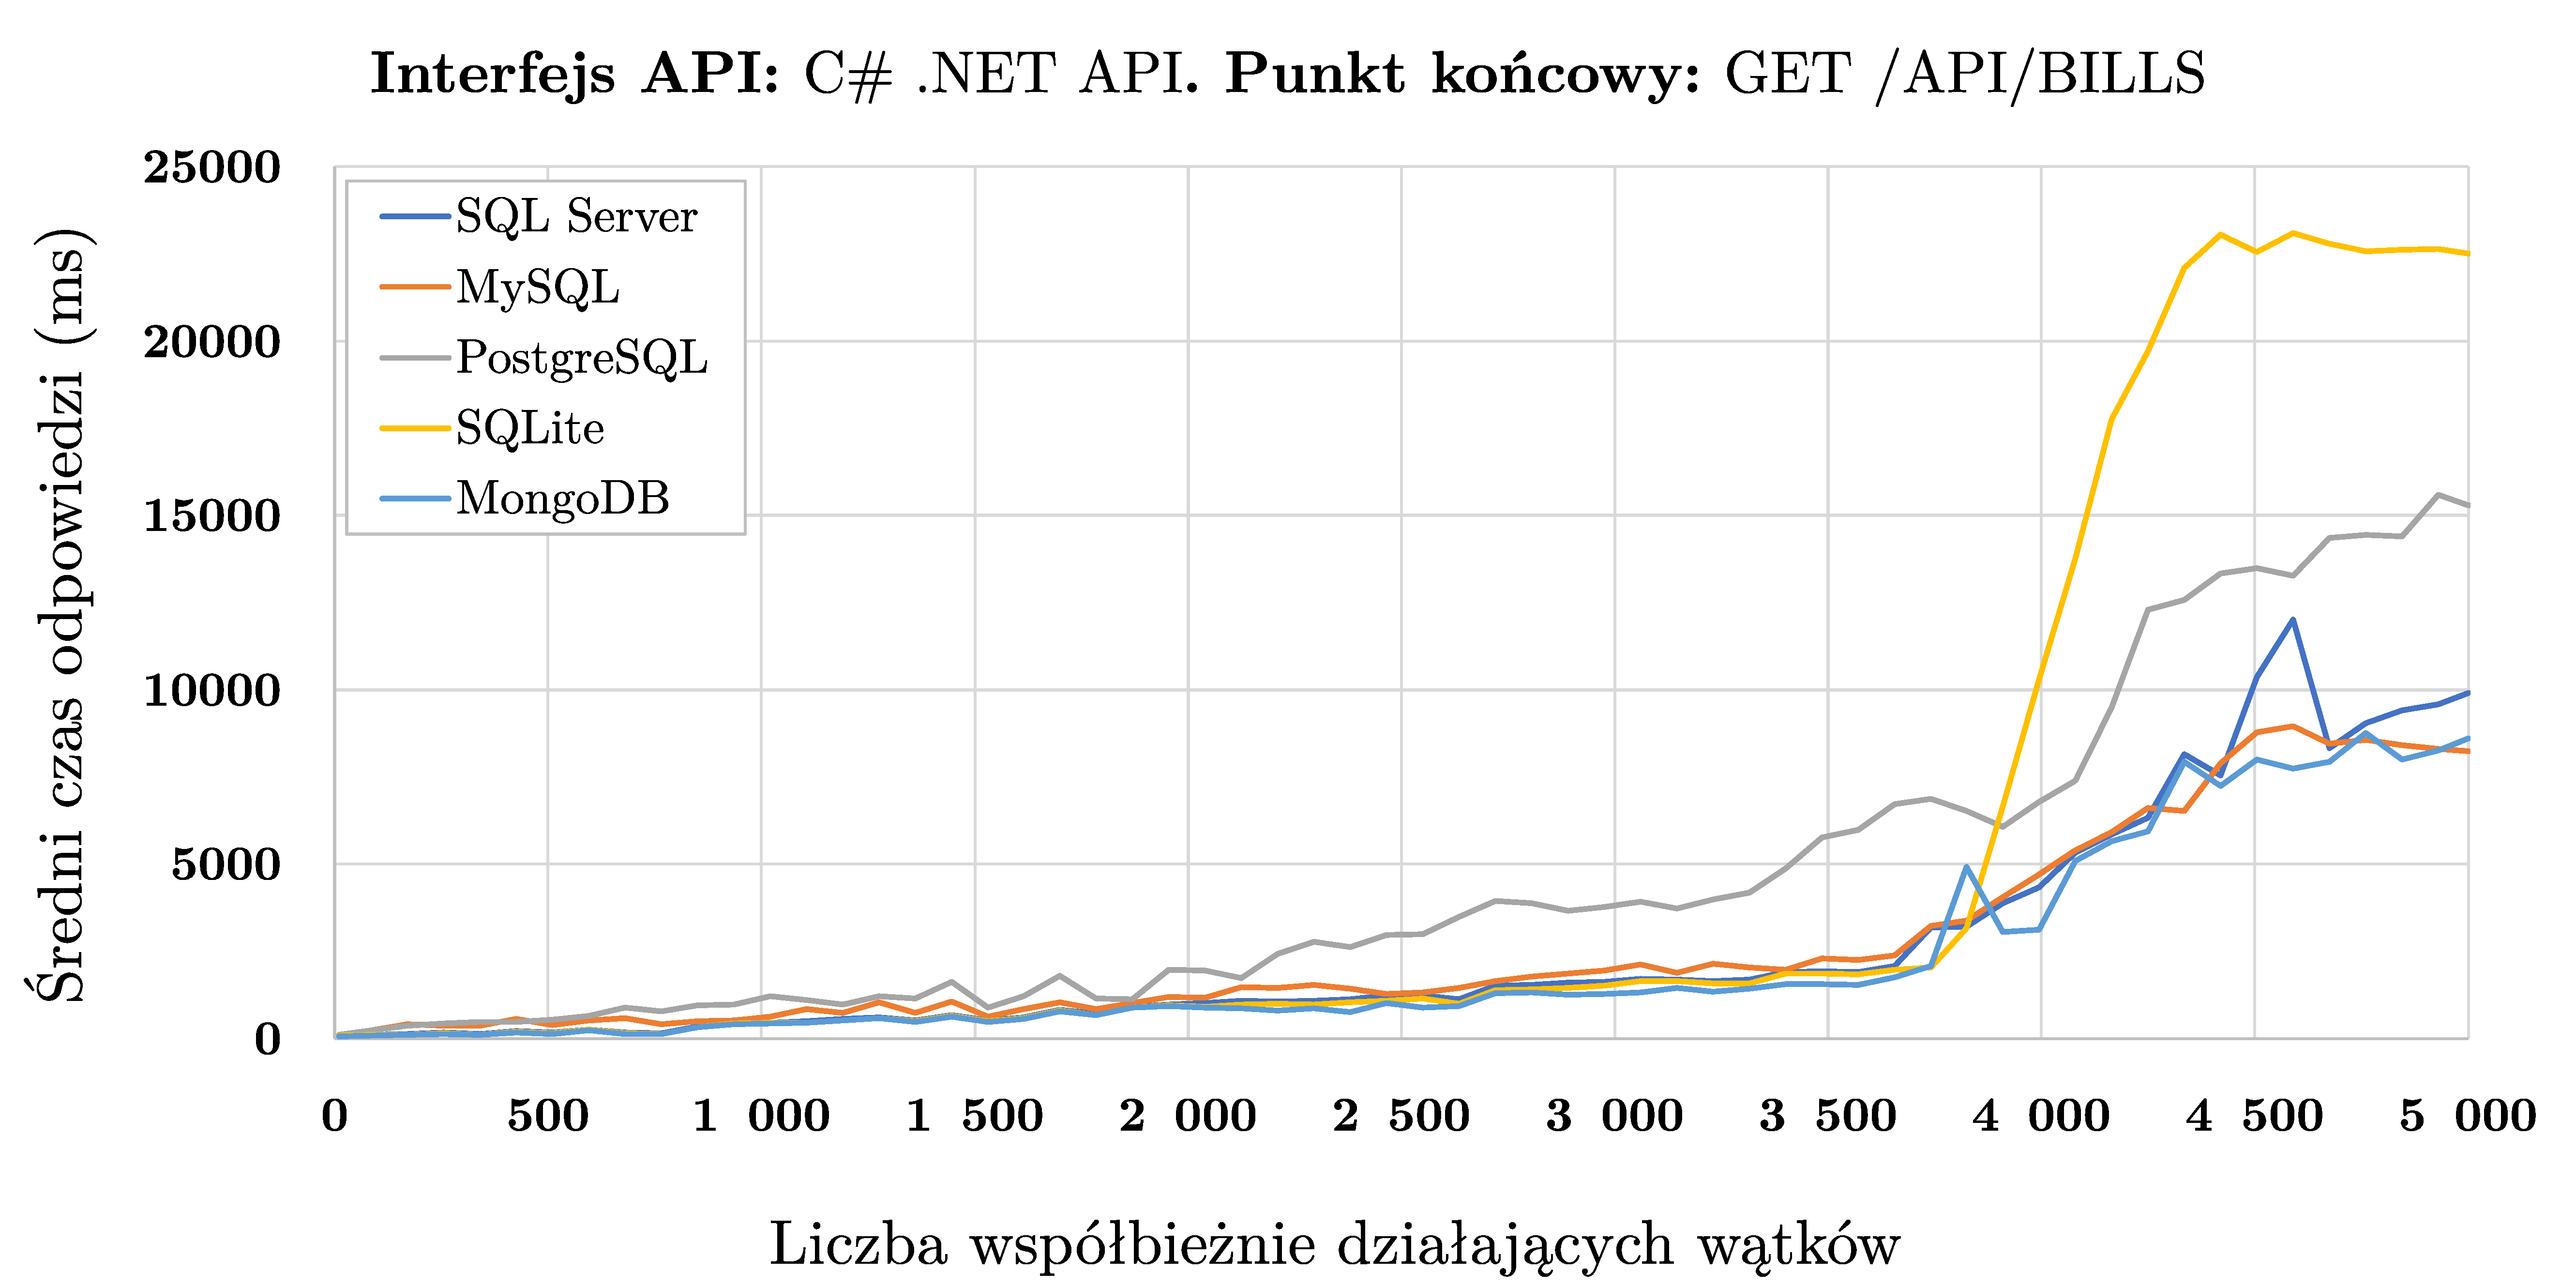
\includegraphics[width=0.49\textwidth]{rys05/response-dotnet-fetchAllBills.pdf} & 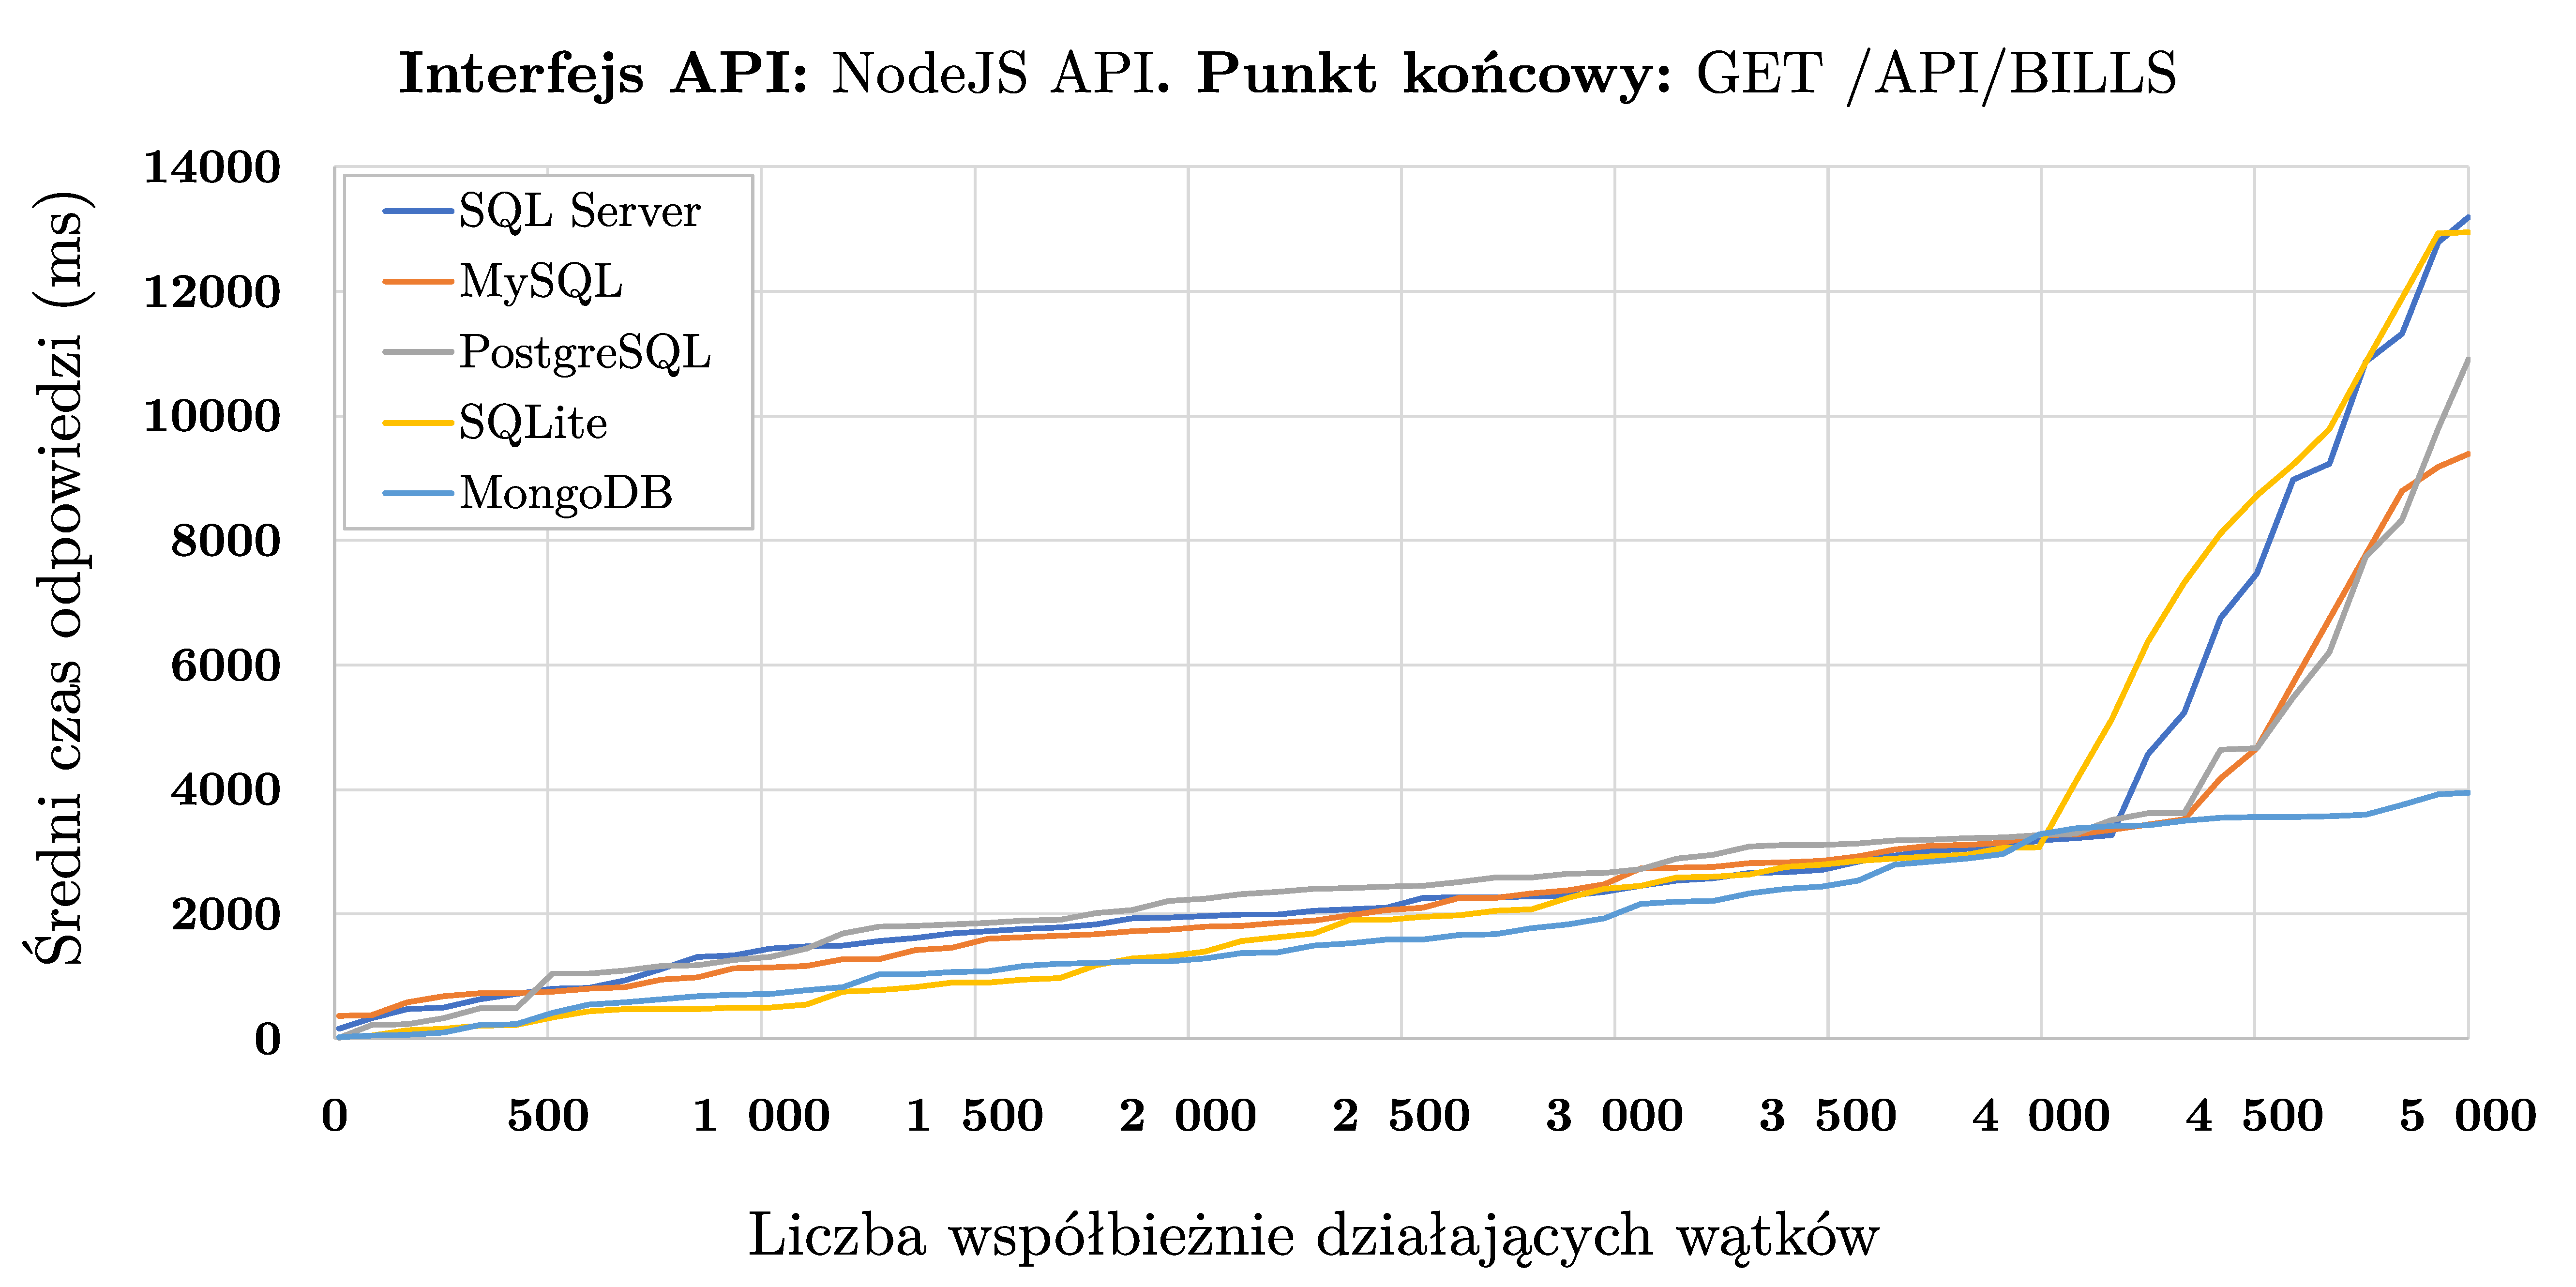
\includegraphics[width=0.49\textwidth]{rys05/response-nodejs-fetchAllBills.pdf} \\
    c) & d) \\
    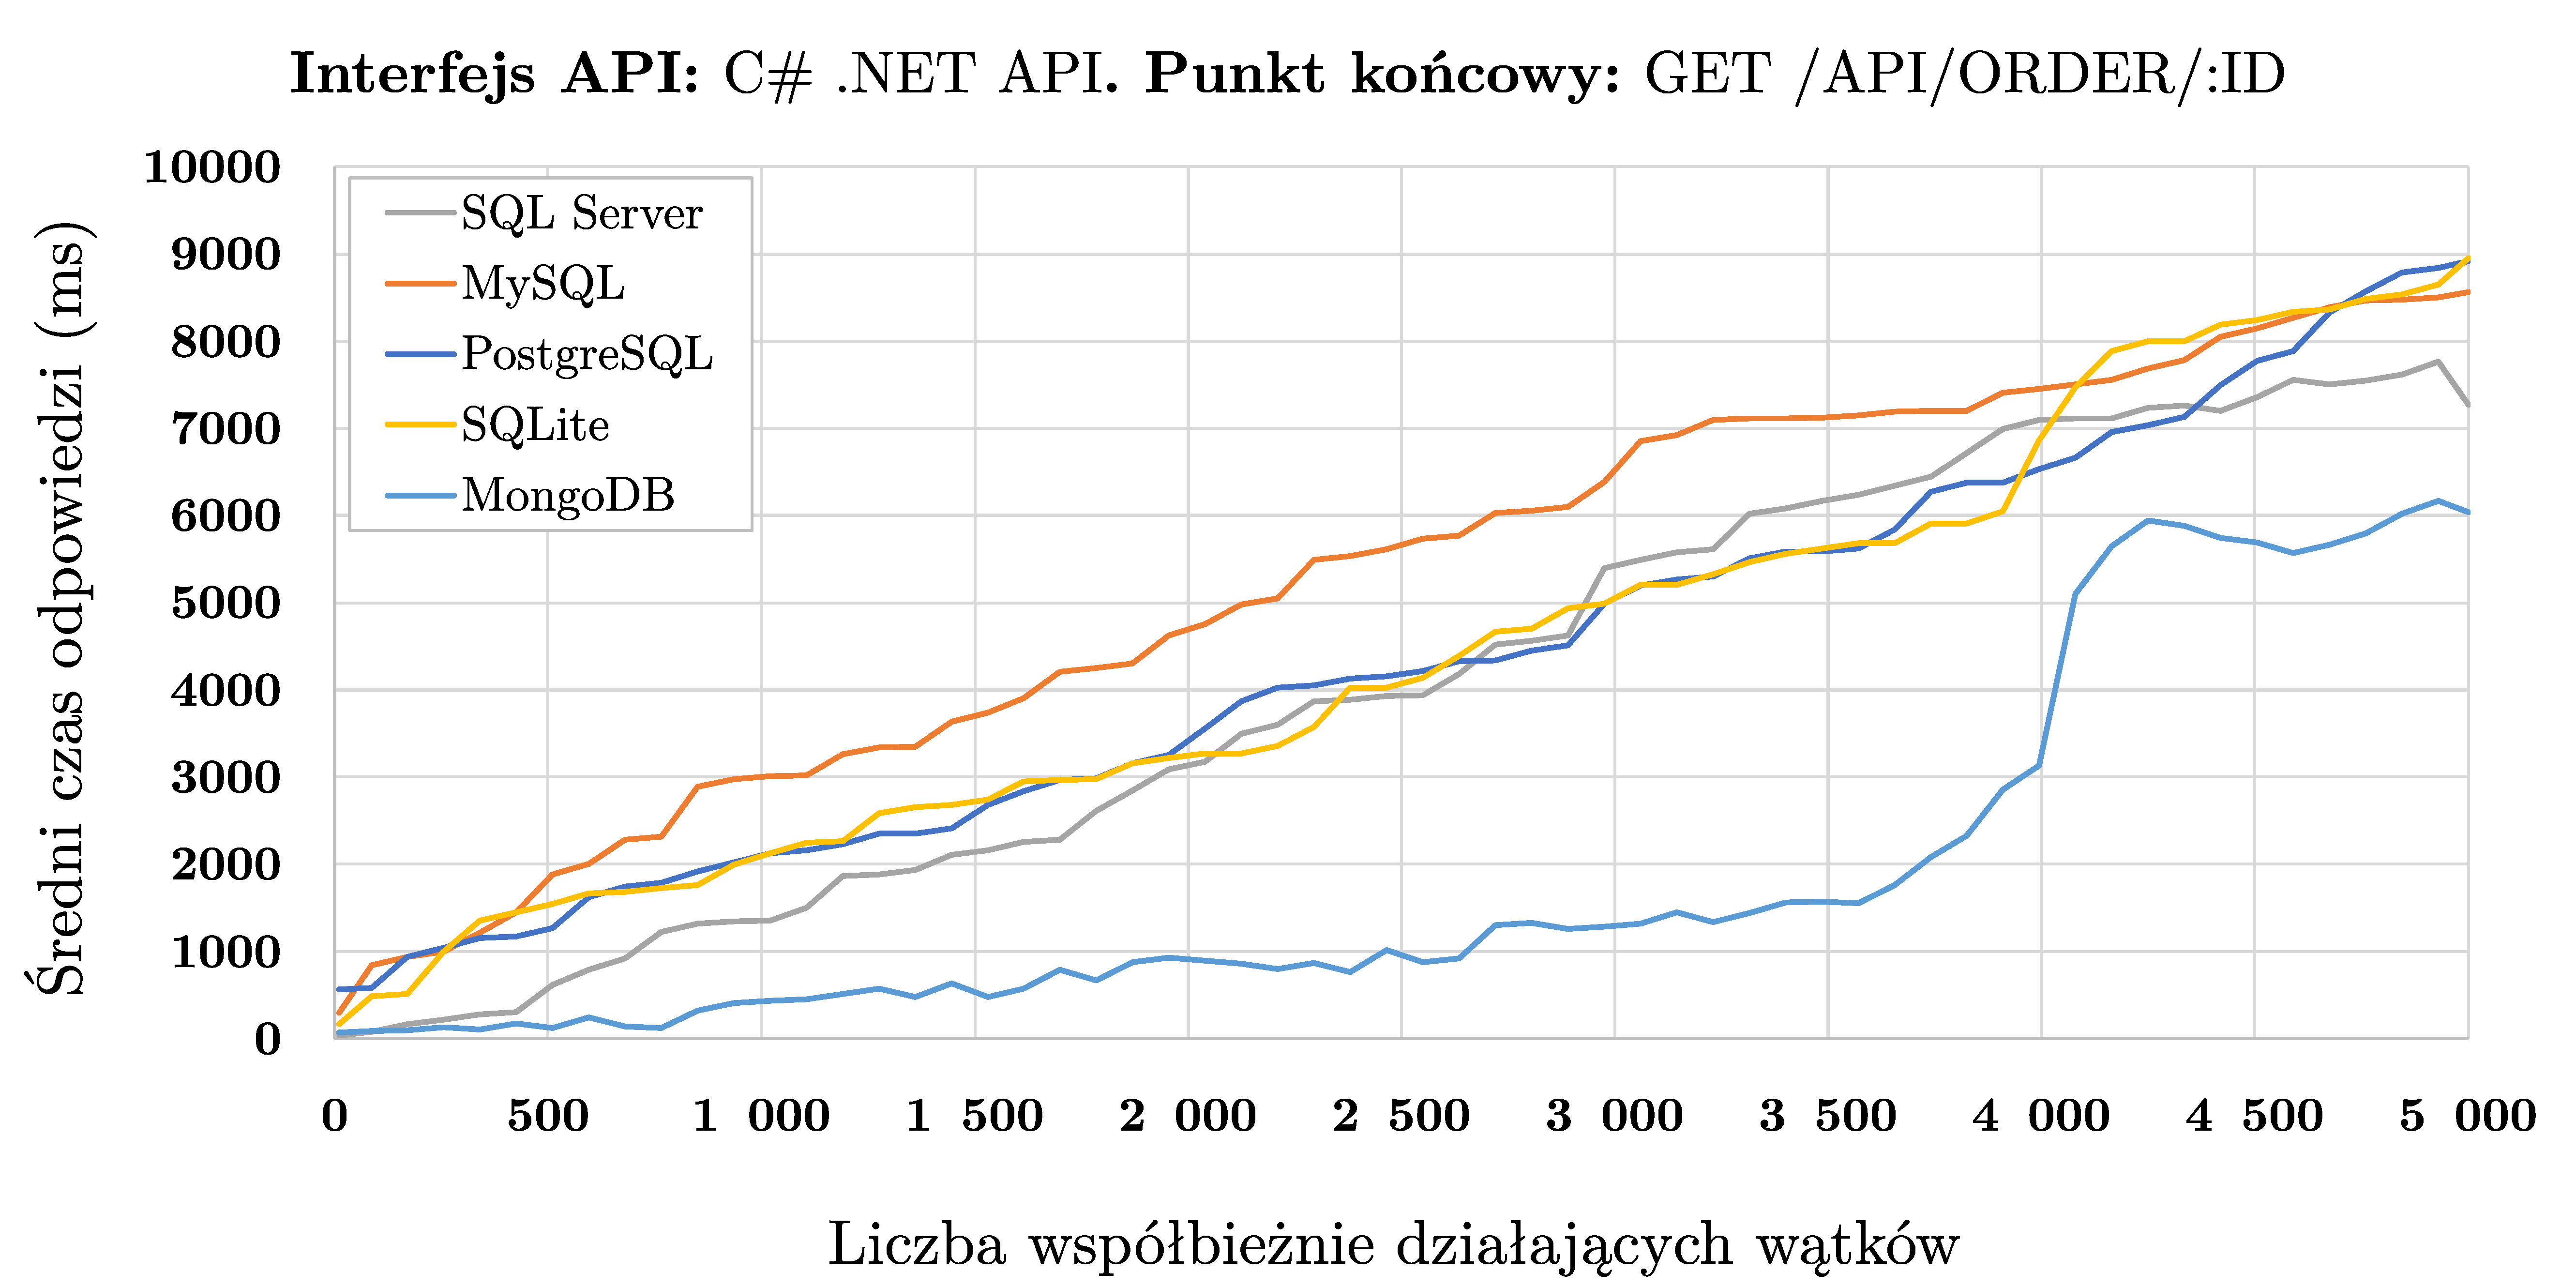
\includegraphics[width=0.49\textwidth]{rys05/response-dotnet-getSingleOrder.pdf} & 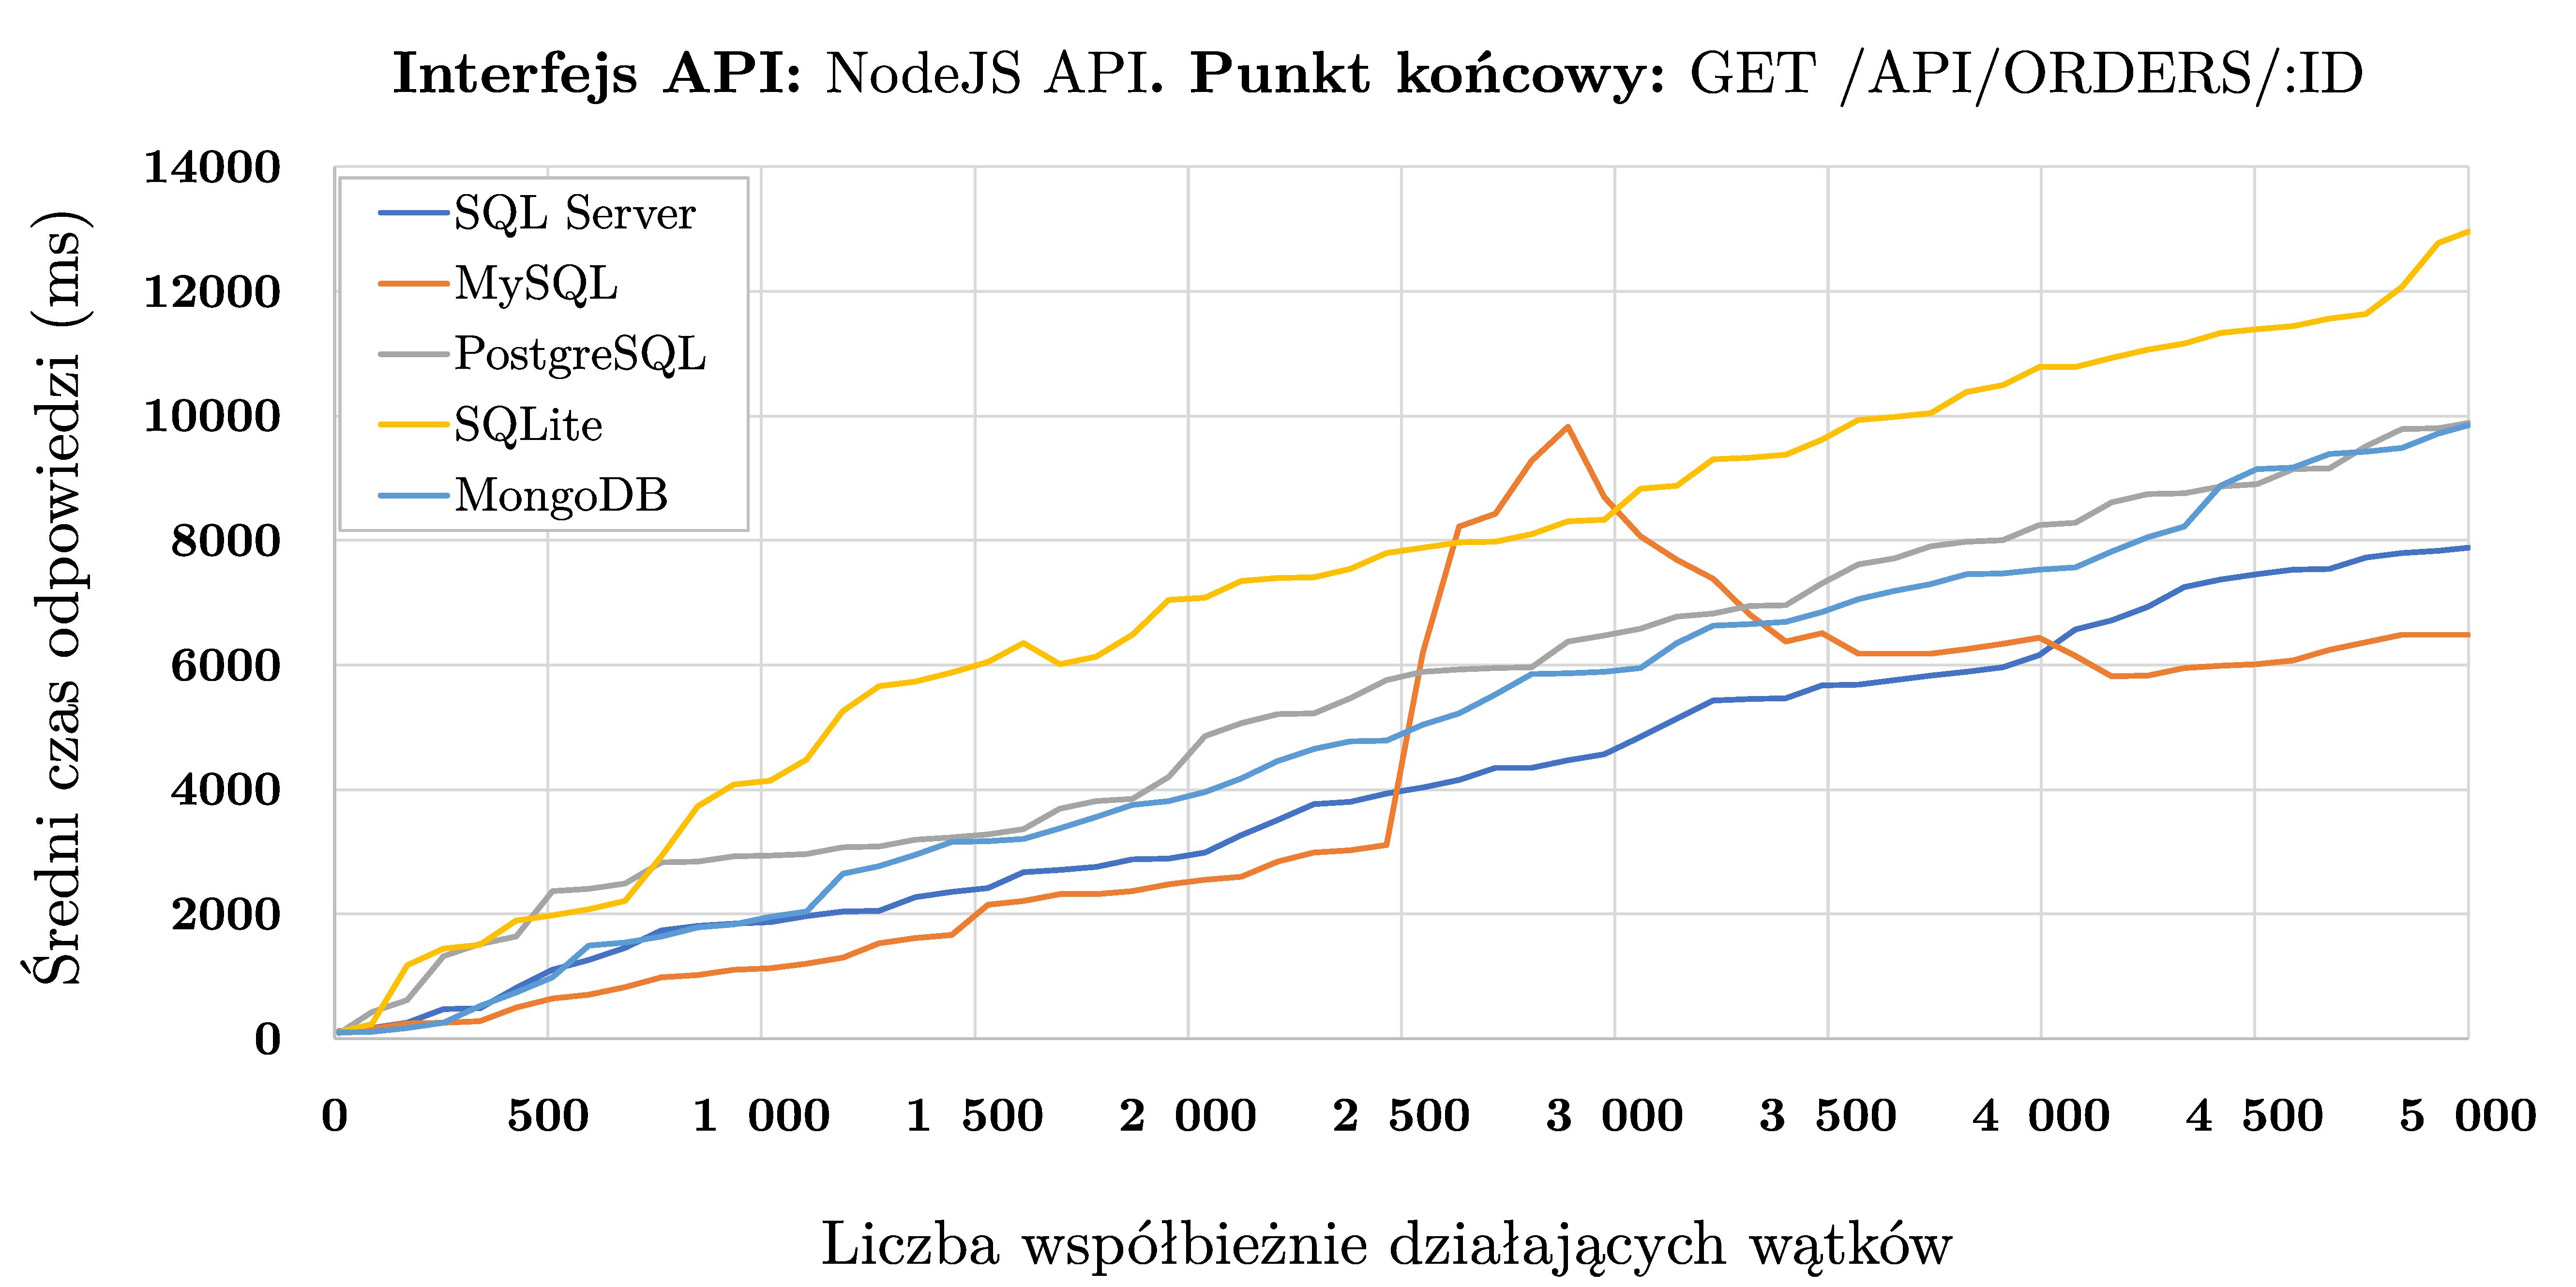
\includegraphics[width=0.49\textwidth]{rys05/response-nodejs-getSingleOrder.pdf} \\
    e) & f) \\
    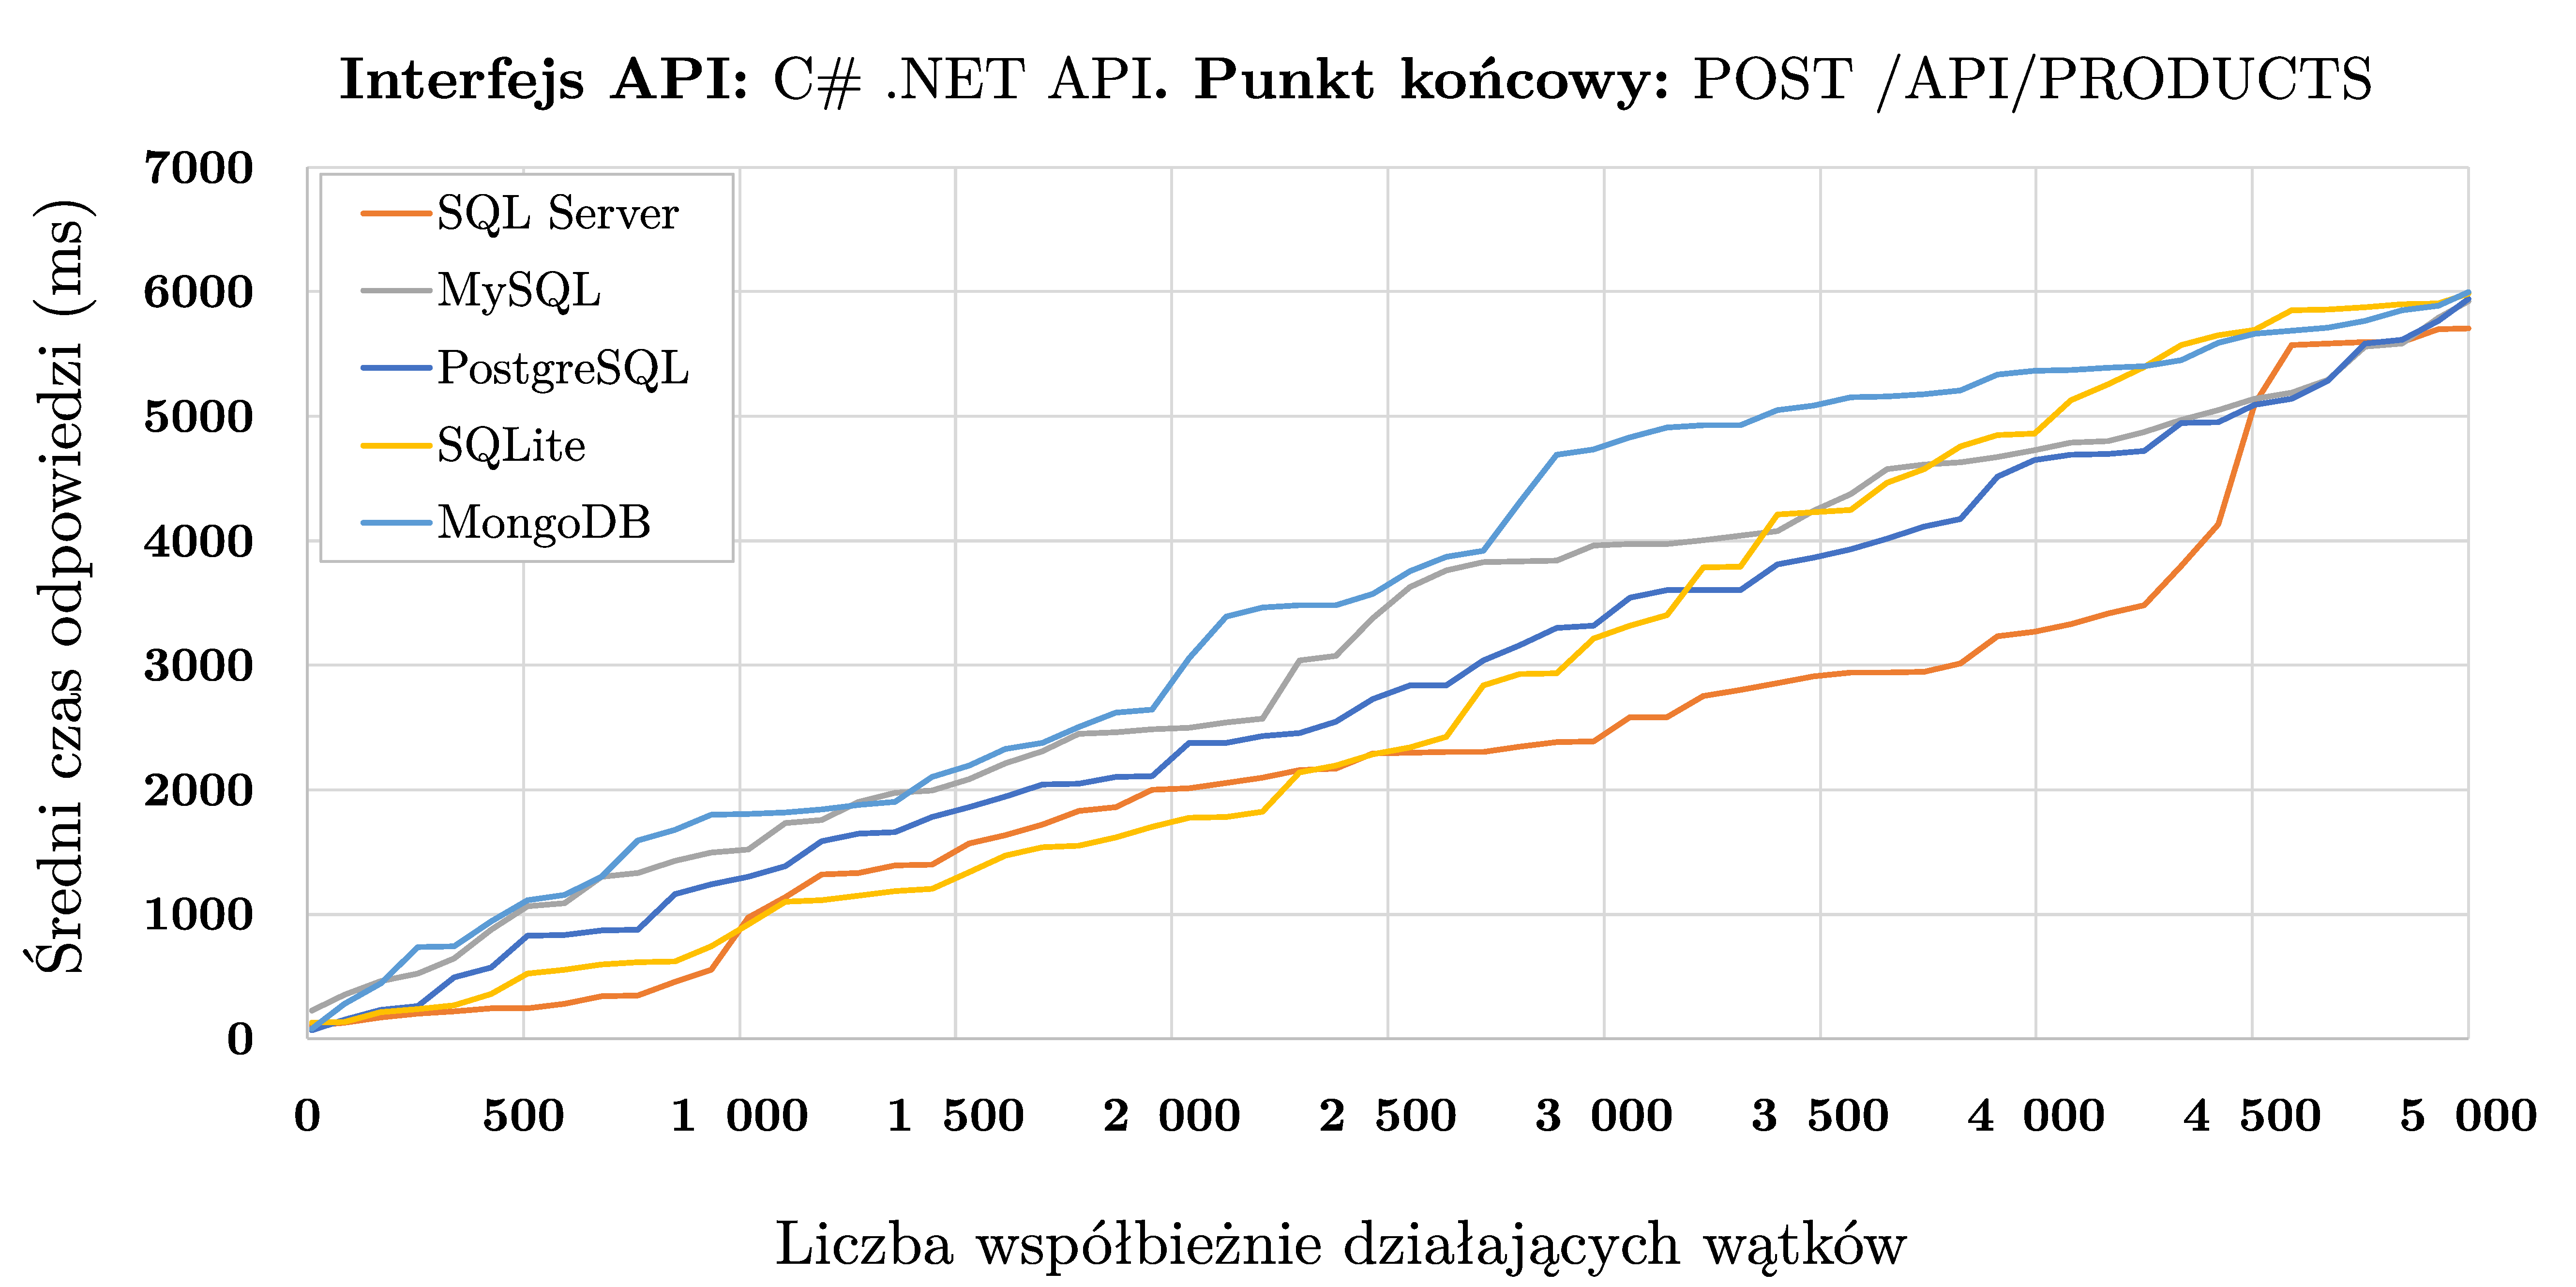
\includegraphics[width=0.49\textwidth]{rys05/response-dotnet-addProduct.pdf} & 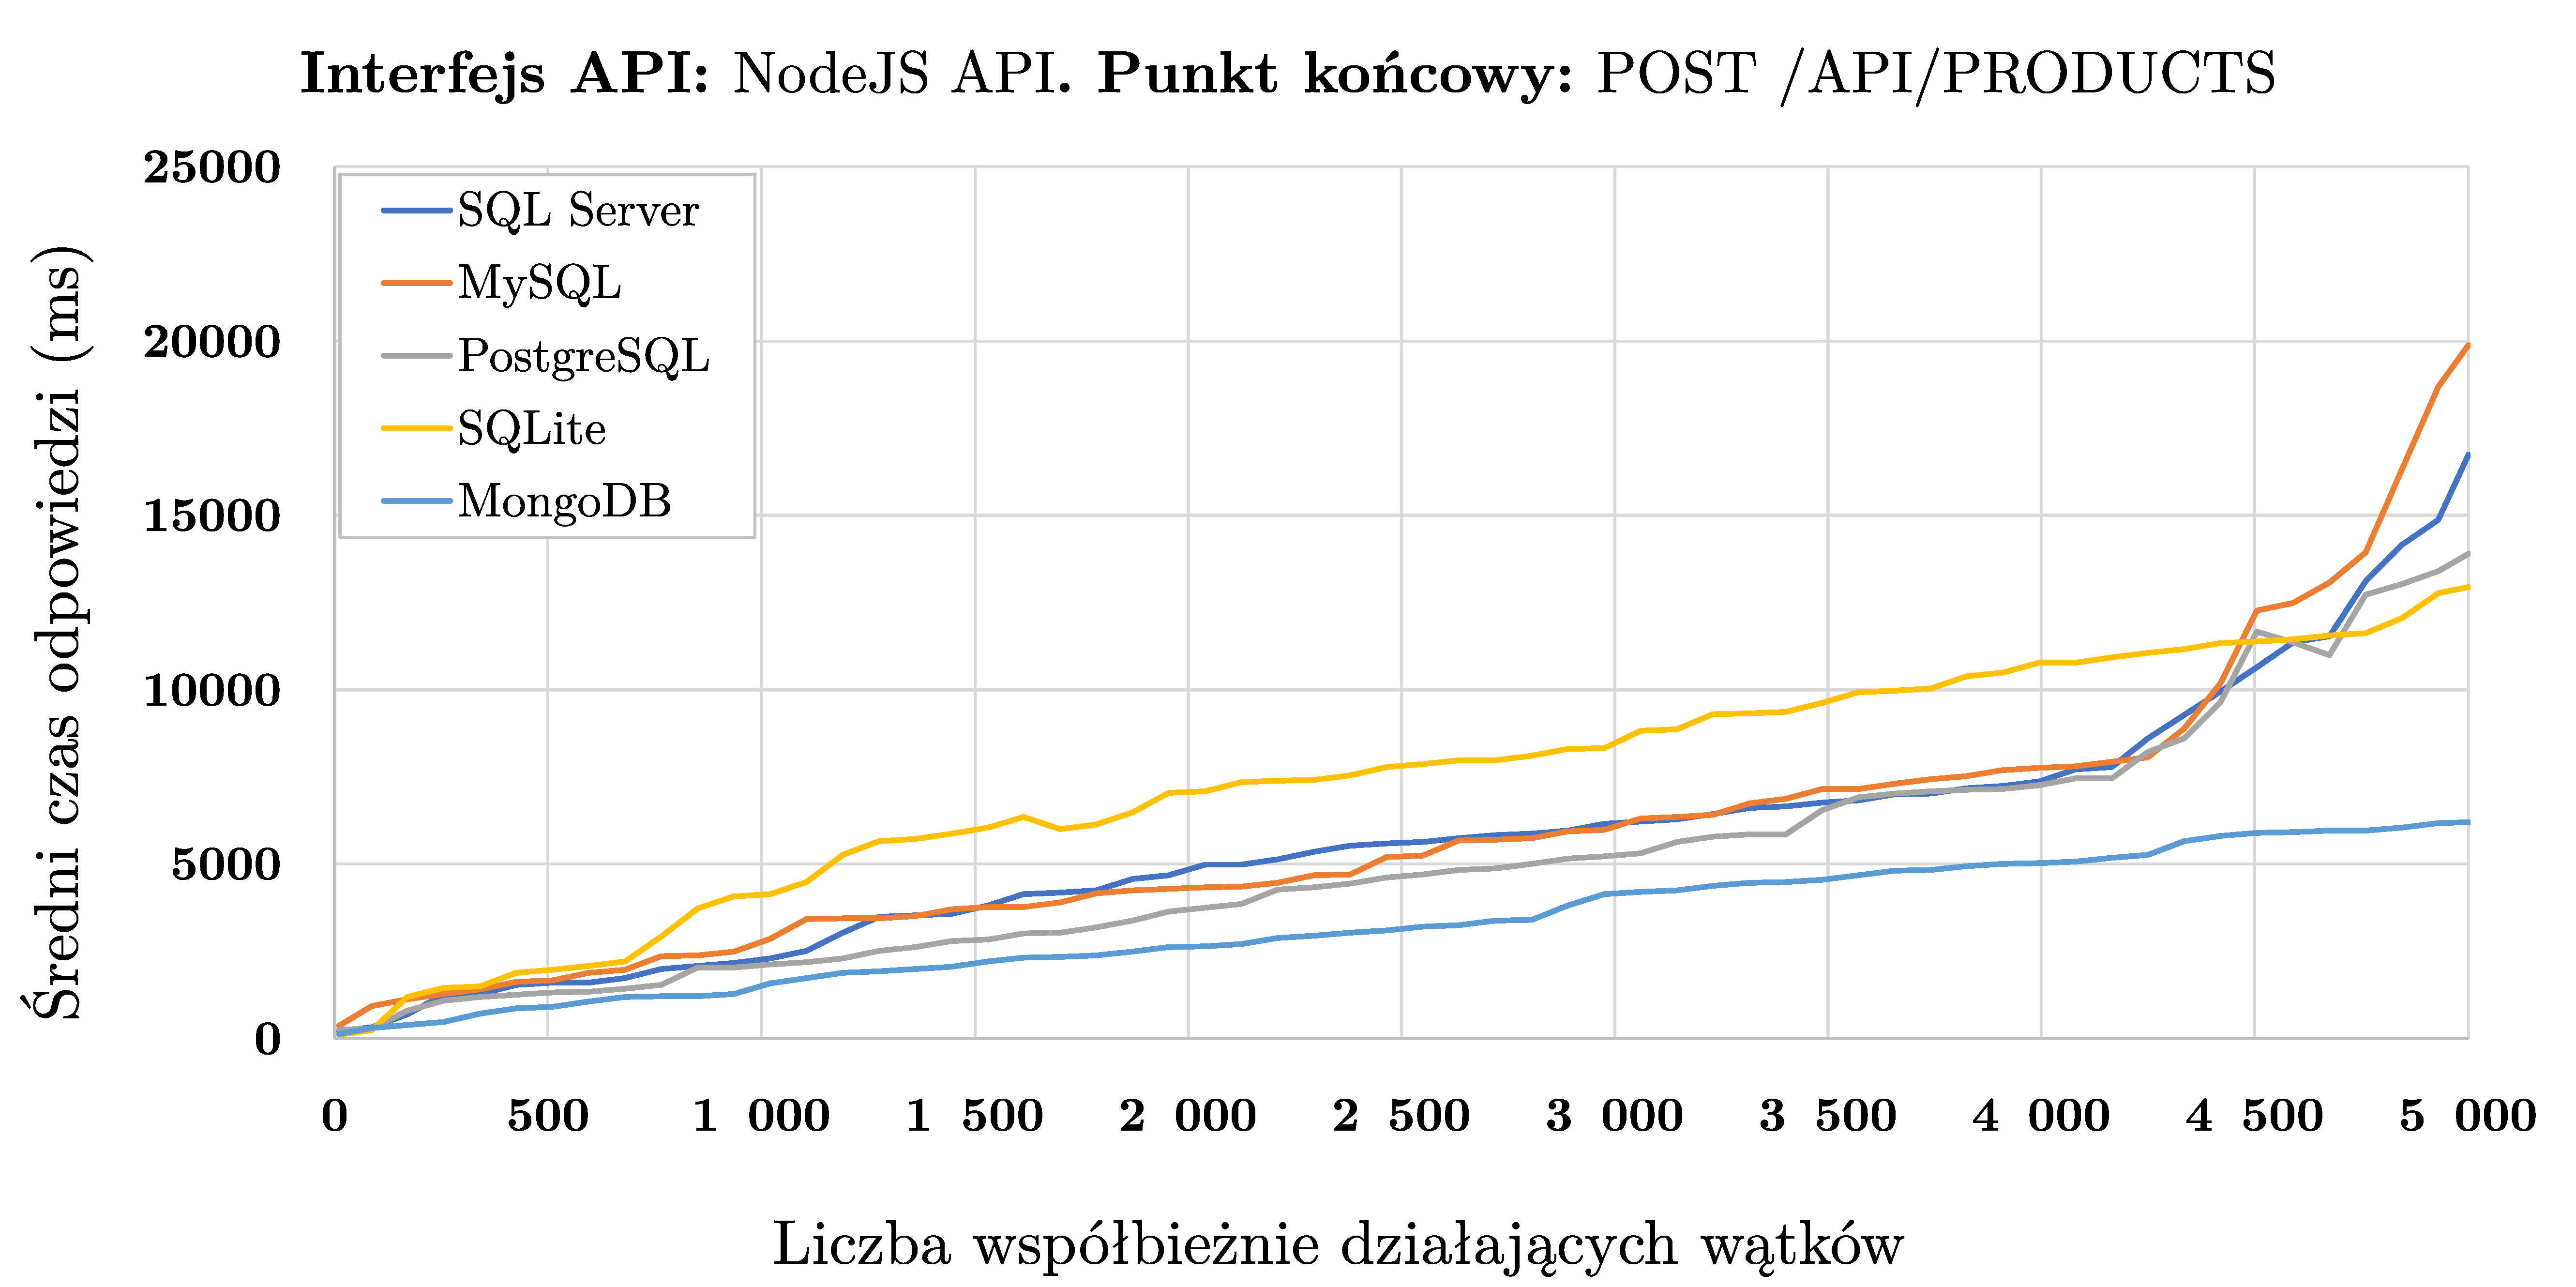
\includegraphics[width=0.49\textwidth]{rys05/response-nodejs-addProduct.pdf} \\
    g) & h) \\
    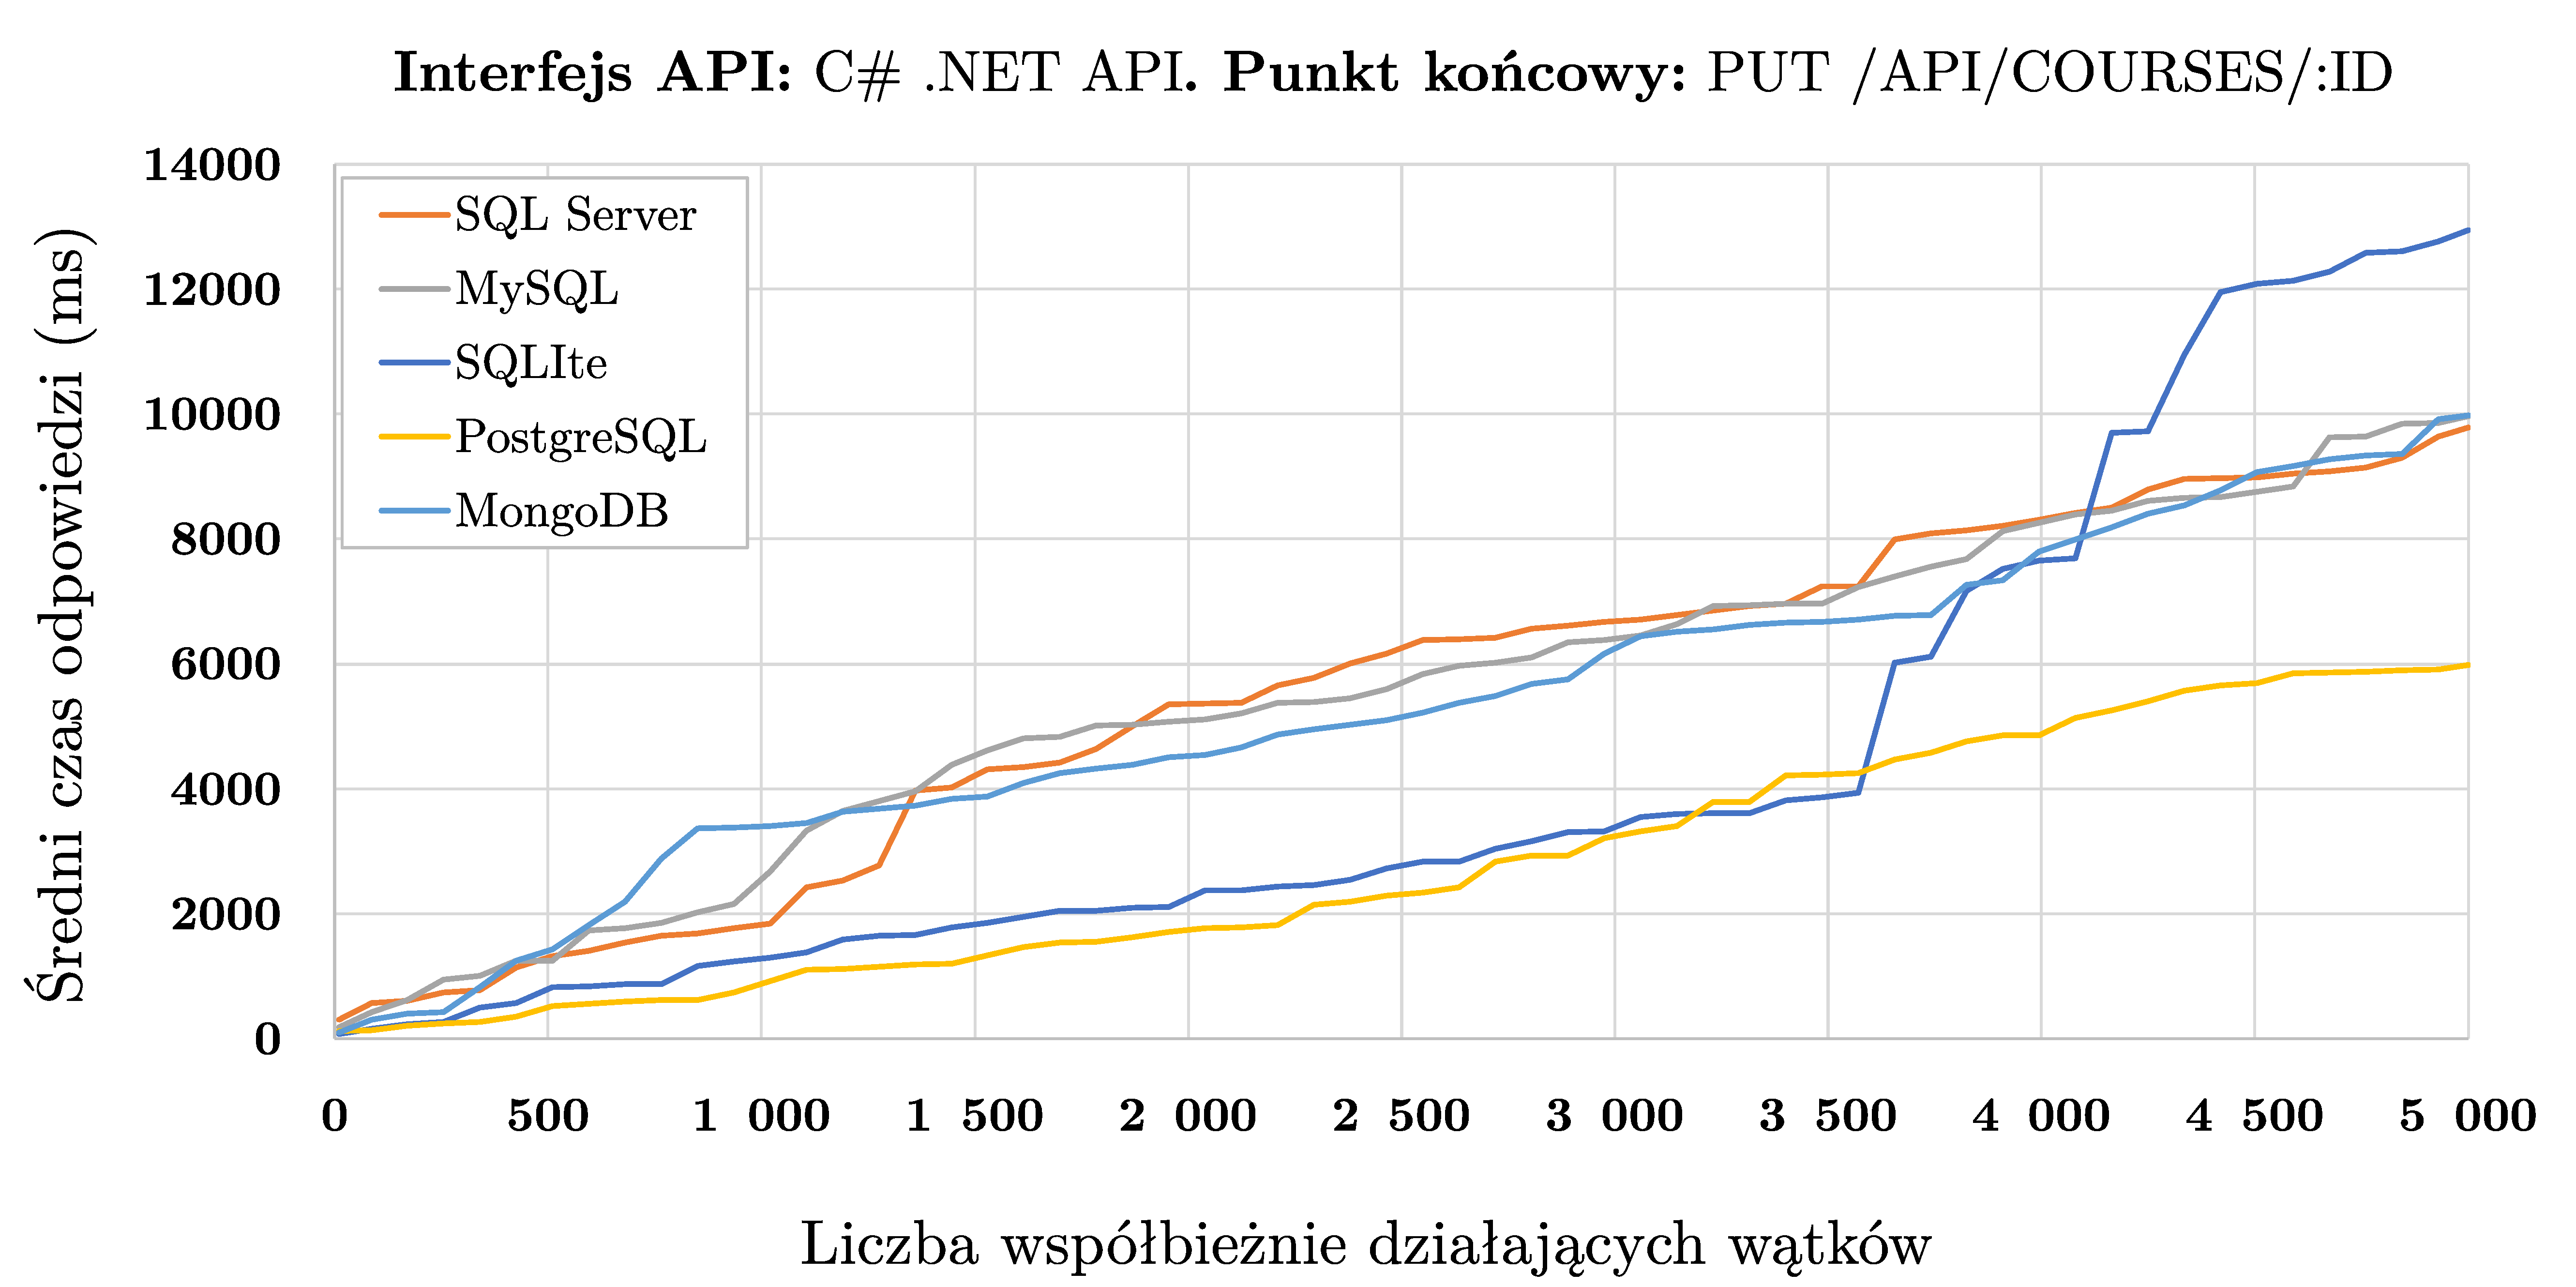
\includegraphics[width=0.49\textwidth]{rys05/response-dotnet-updateCourse.pdf} & 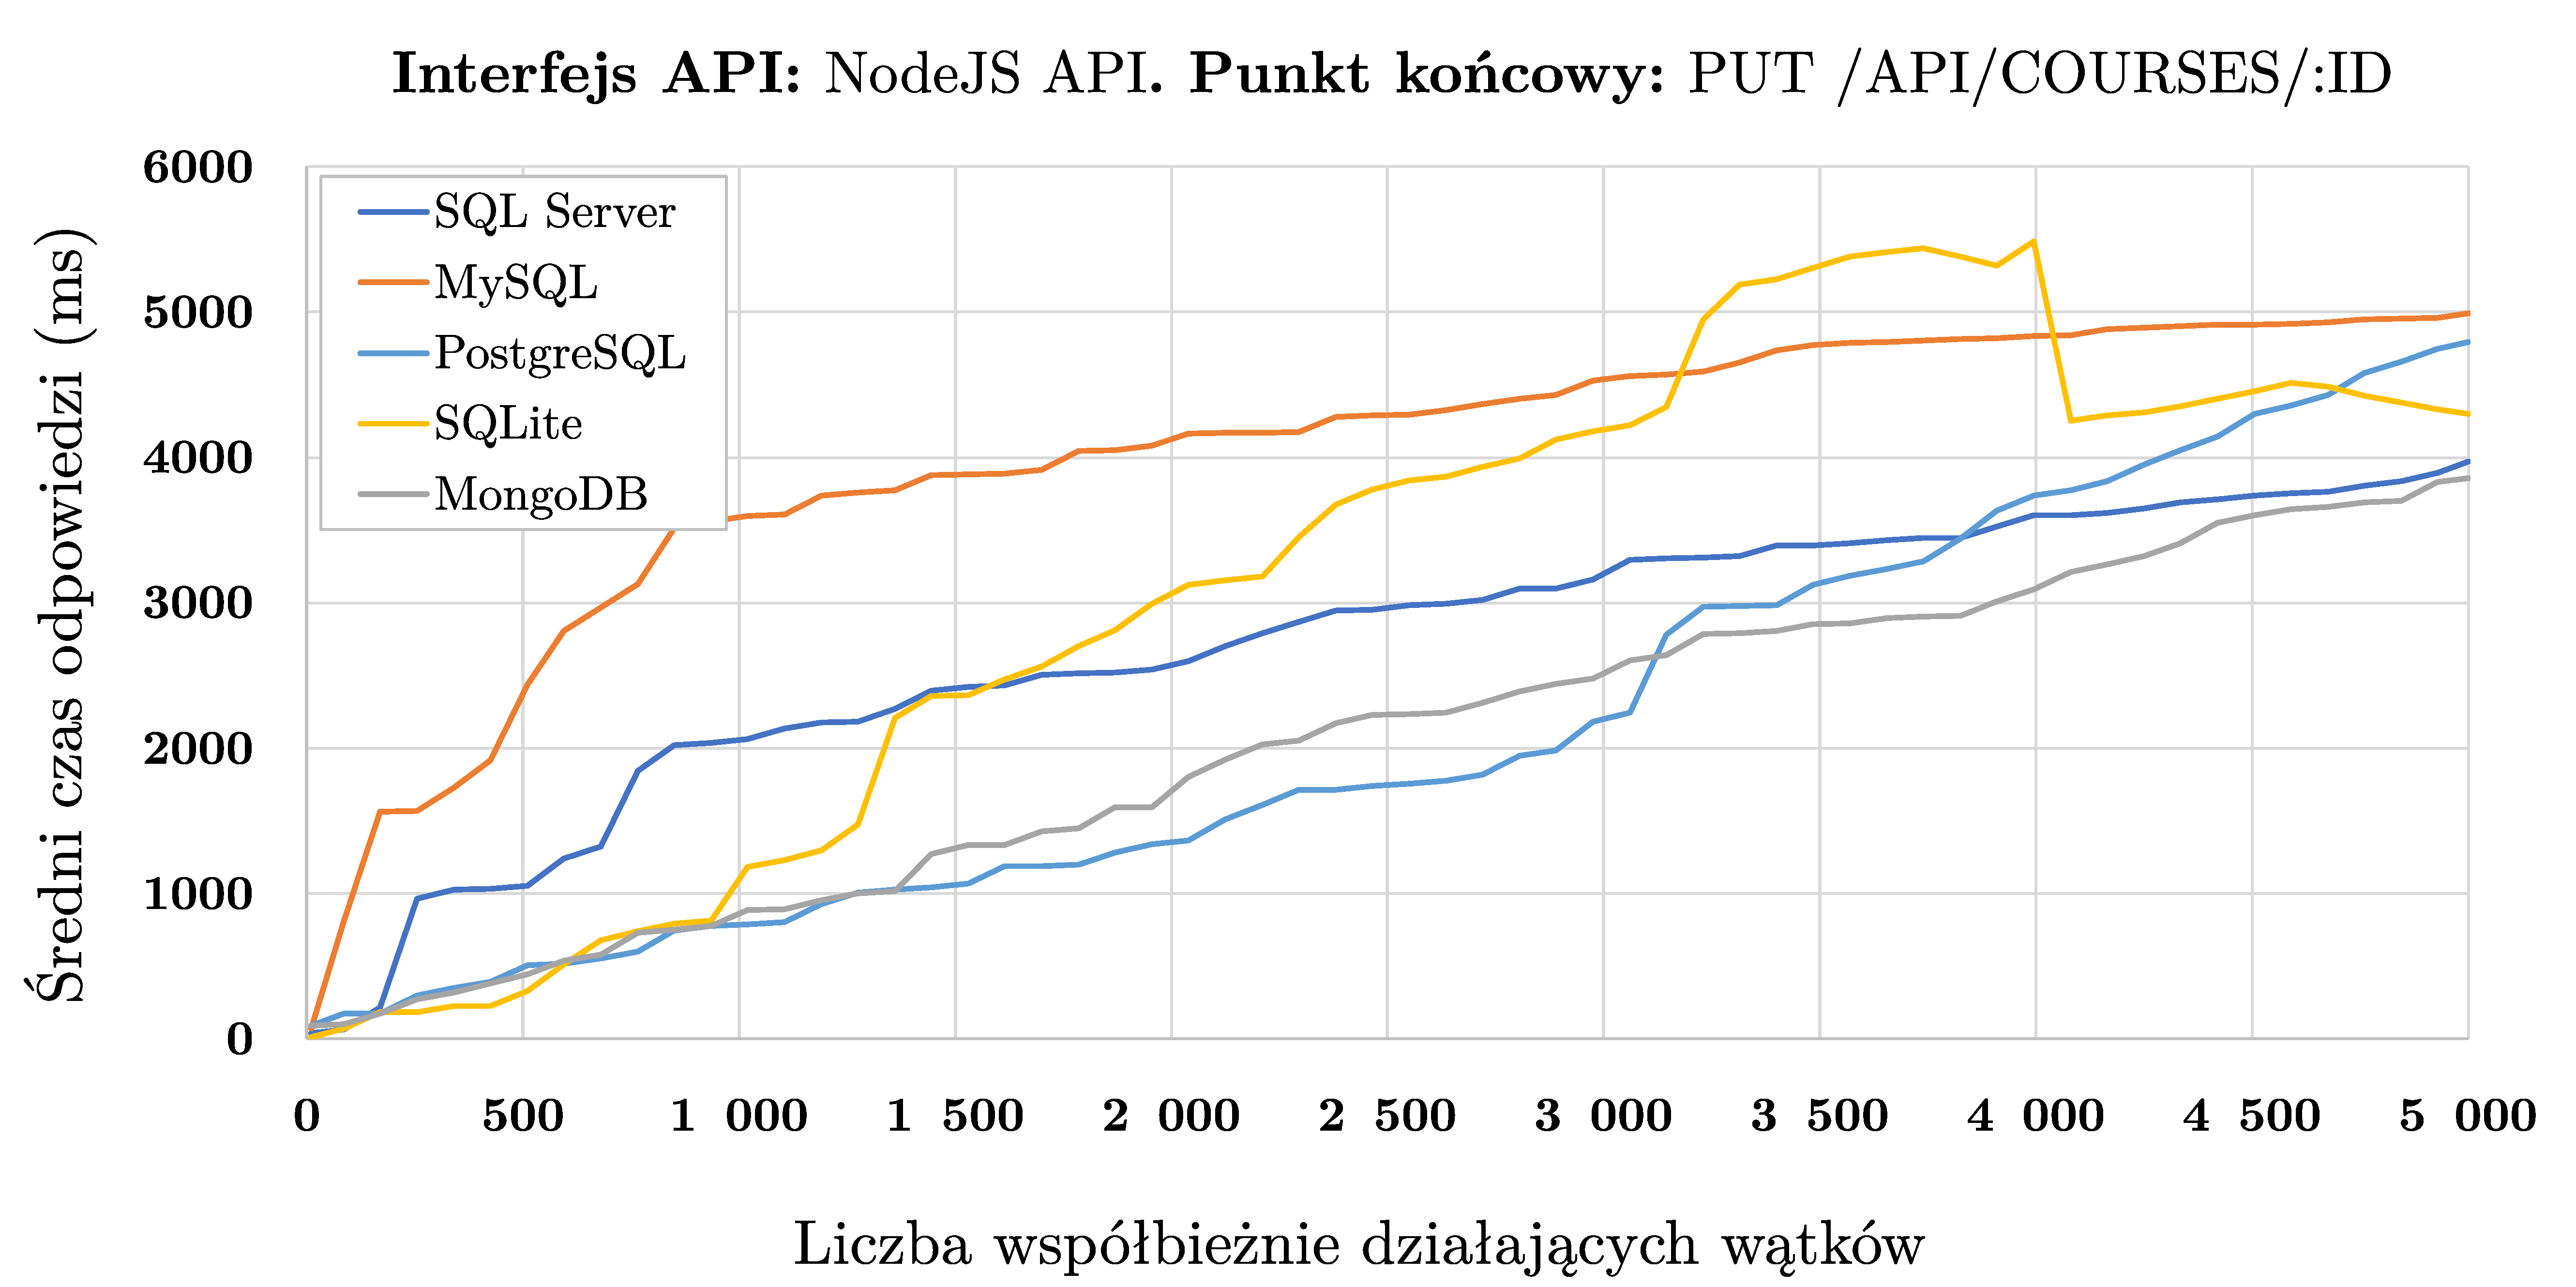
\includegraphics[width=0.49\textwidth]{rys05/response-nodejs-updateCourse.pdf} \\
    i) & j) \\
    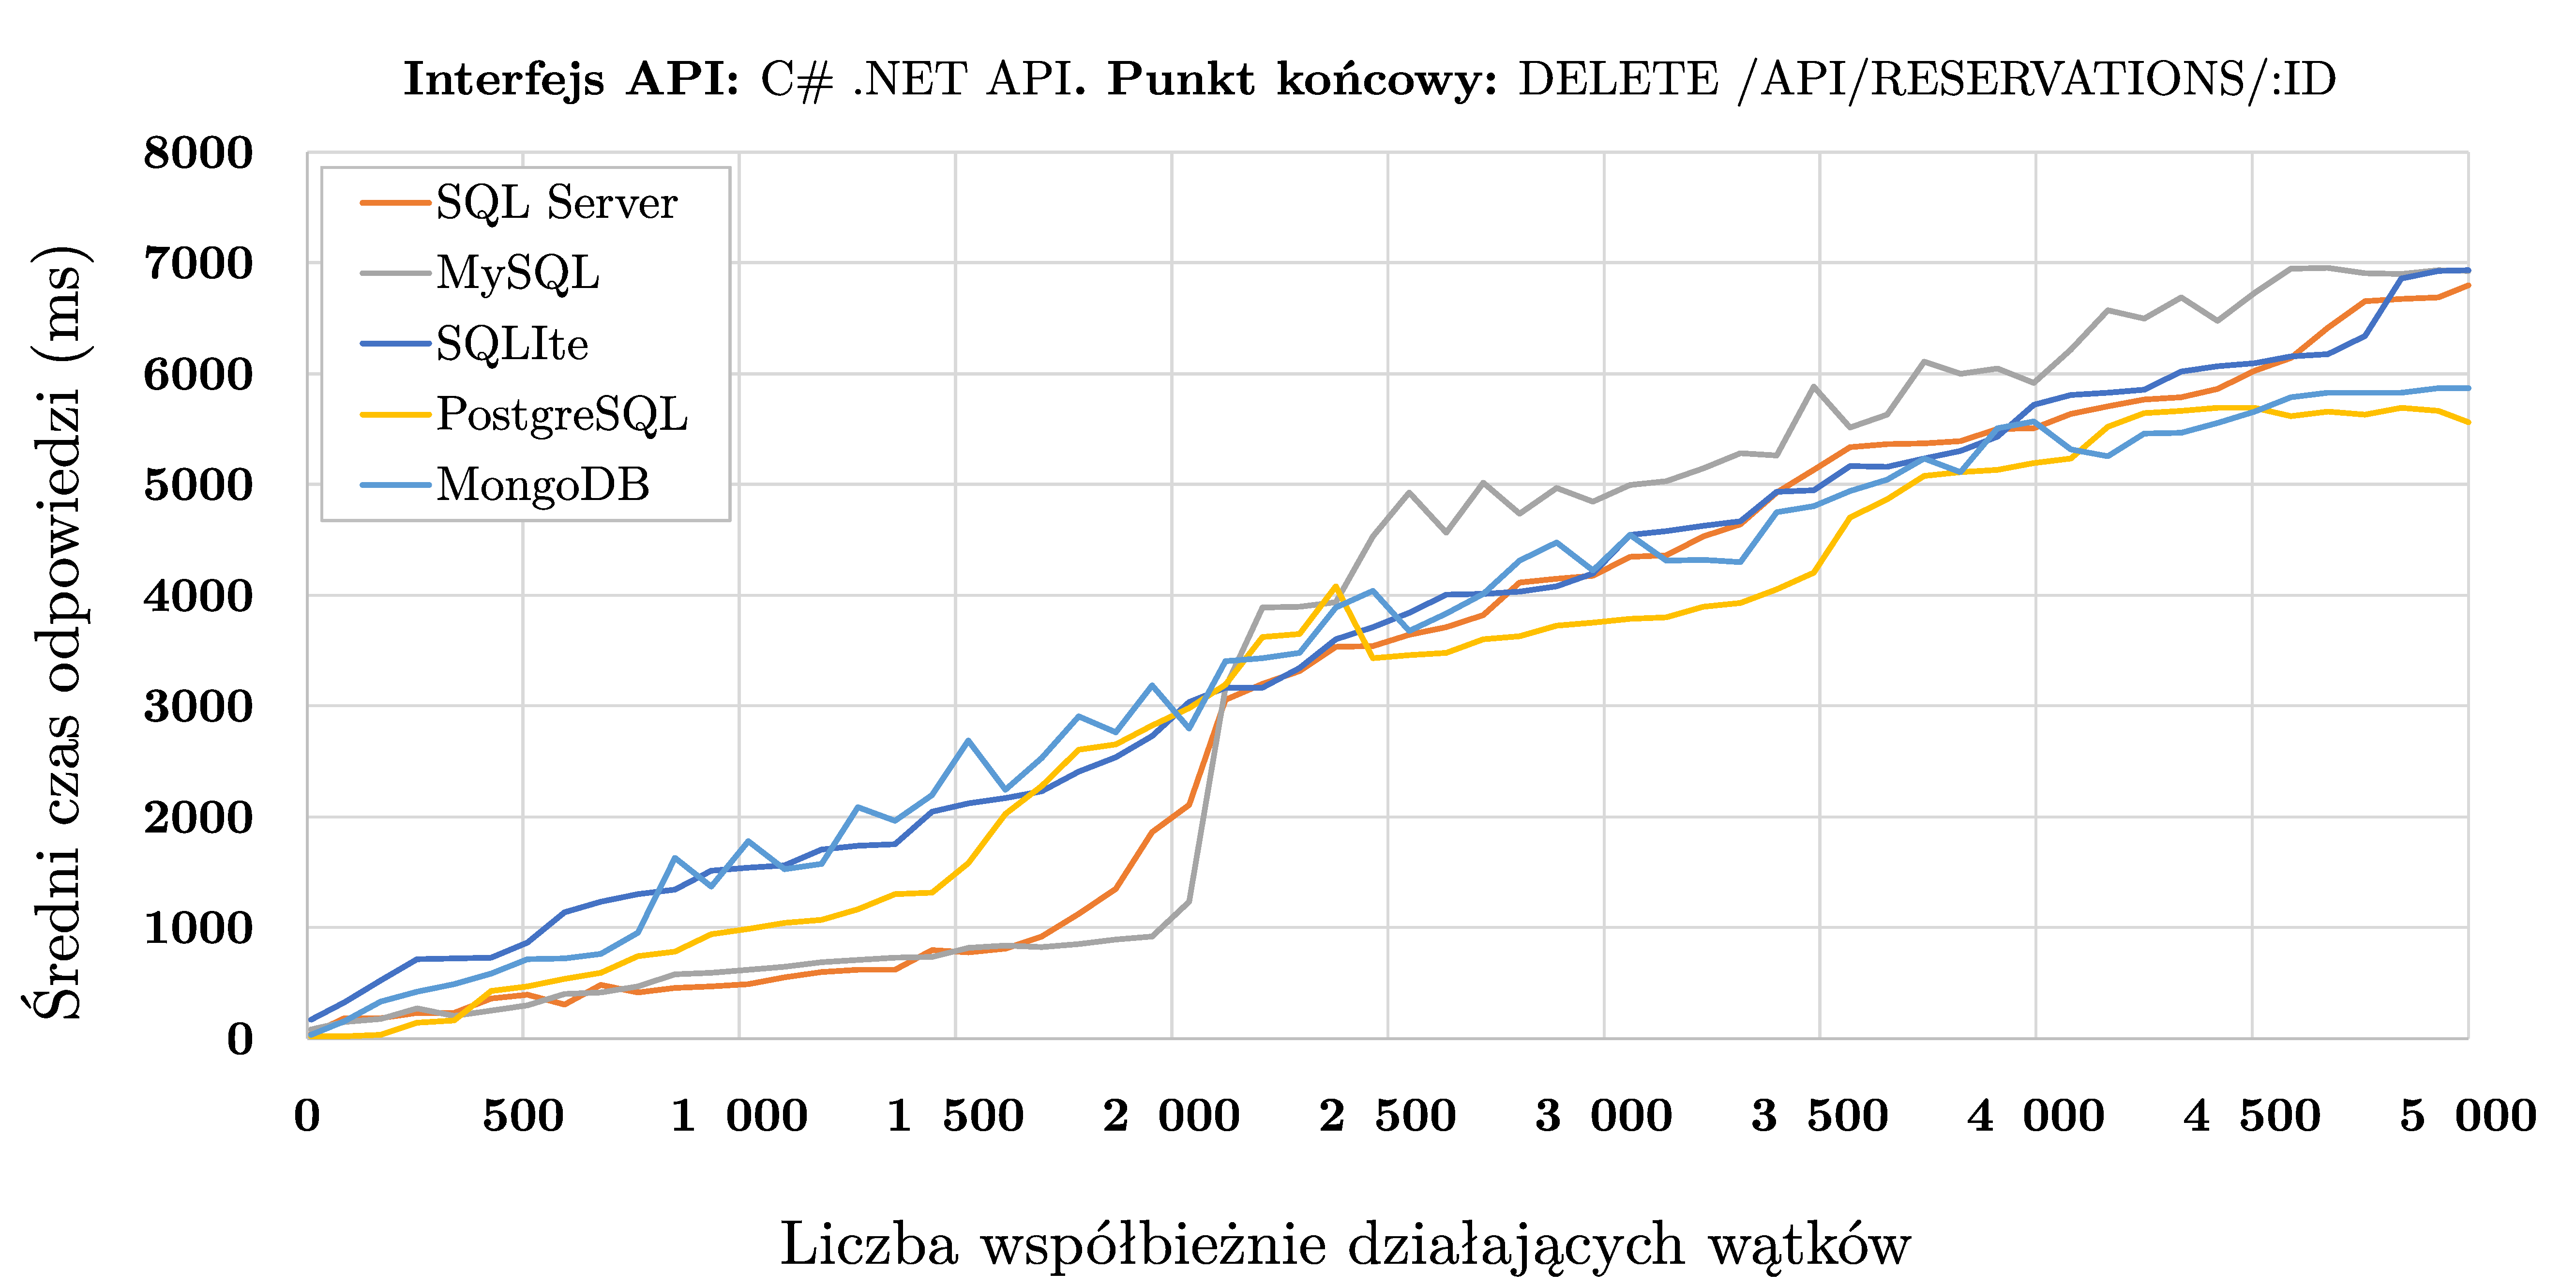
\includegraphics[width=0.49\textwidth]{rys05/response-dotnet-deleteReservation.pdf} & 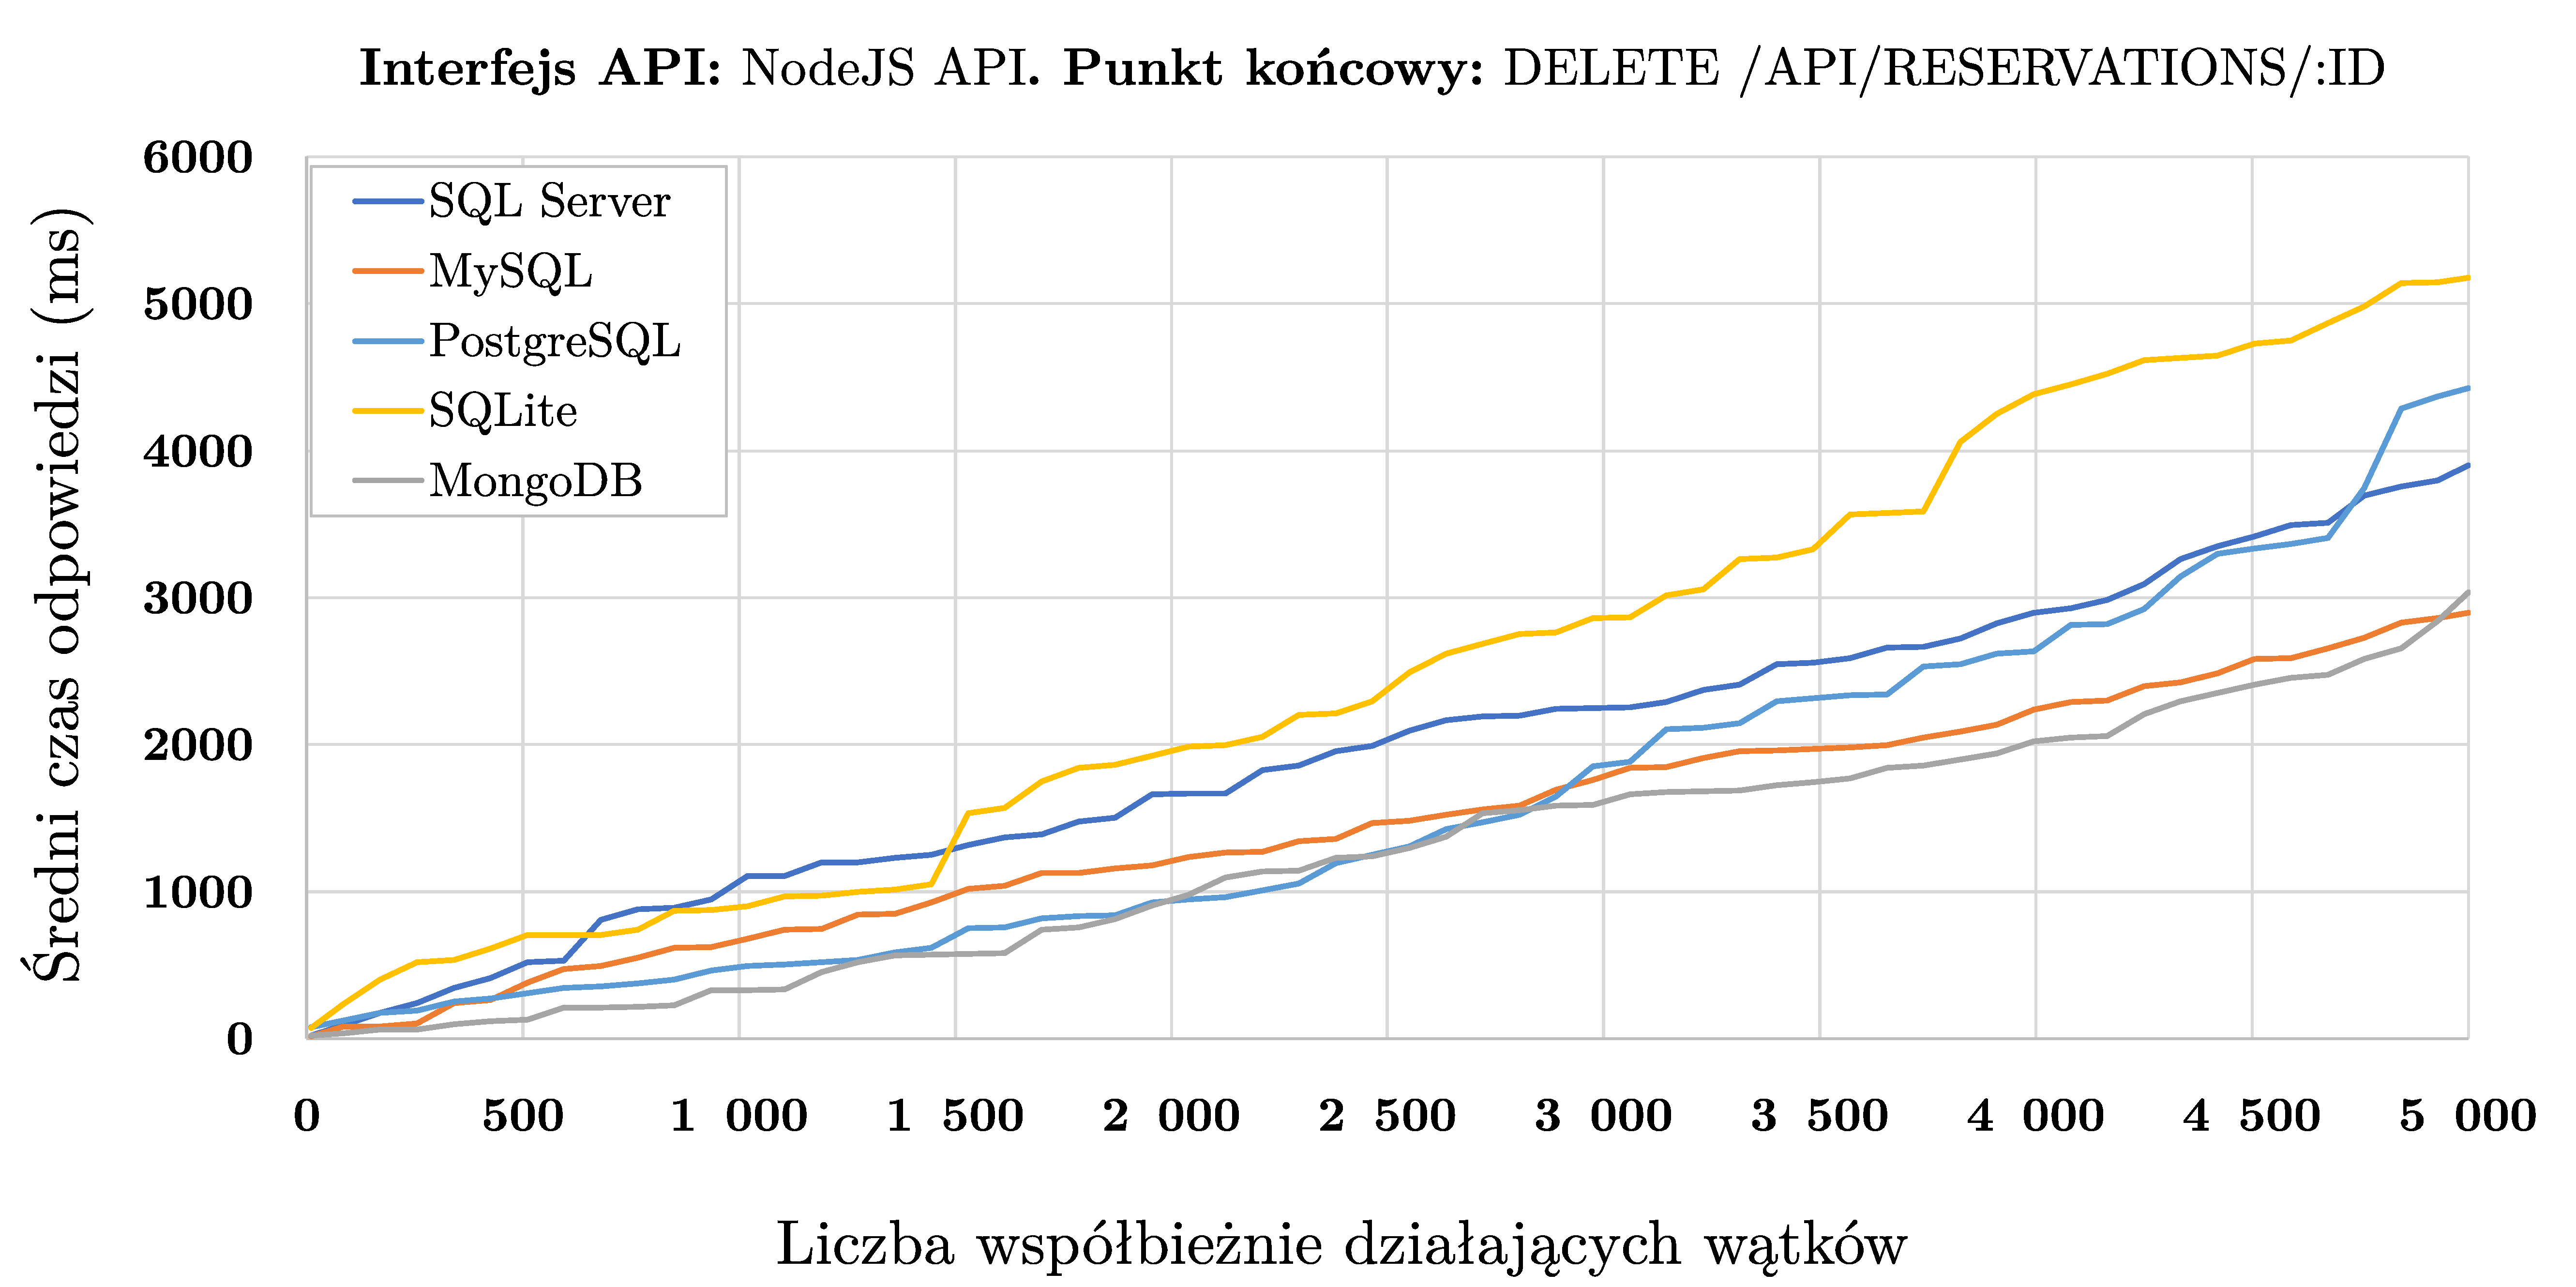
\includegraphics[width=0.49\textwidth]{rys05/response-nodejs-deleteReservation.pdf} \\
	% jezeli obraki sa rownej wysokosci, mozna je wyrownac do gory stosujac vtop jak nizej
	% \vtop{\vskip-2ex\hbox{{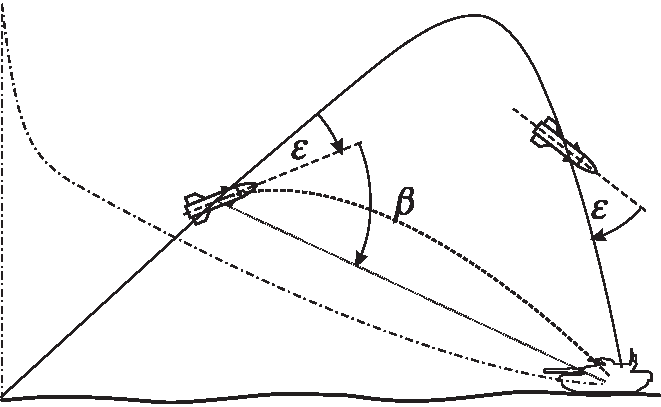
\includegraphics[width=0.475\textwidth]{rys05/beta1}}}} &
	% \vtop{\vskip-2ex\hbox{{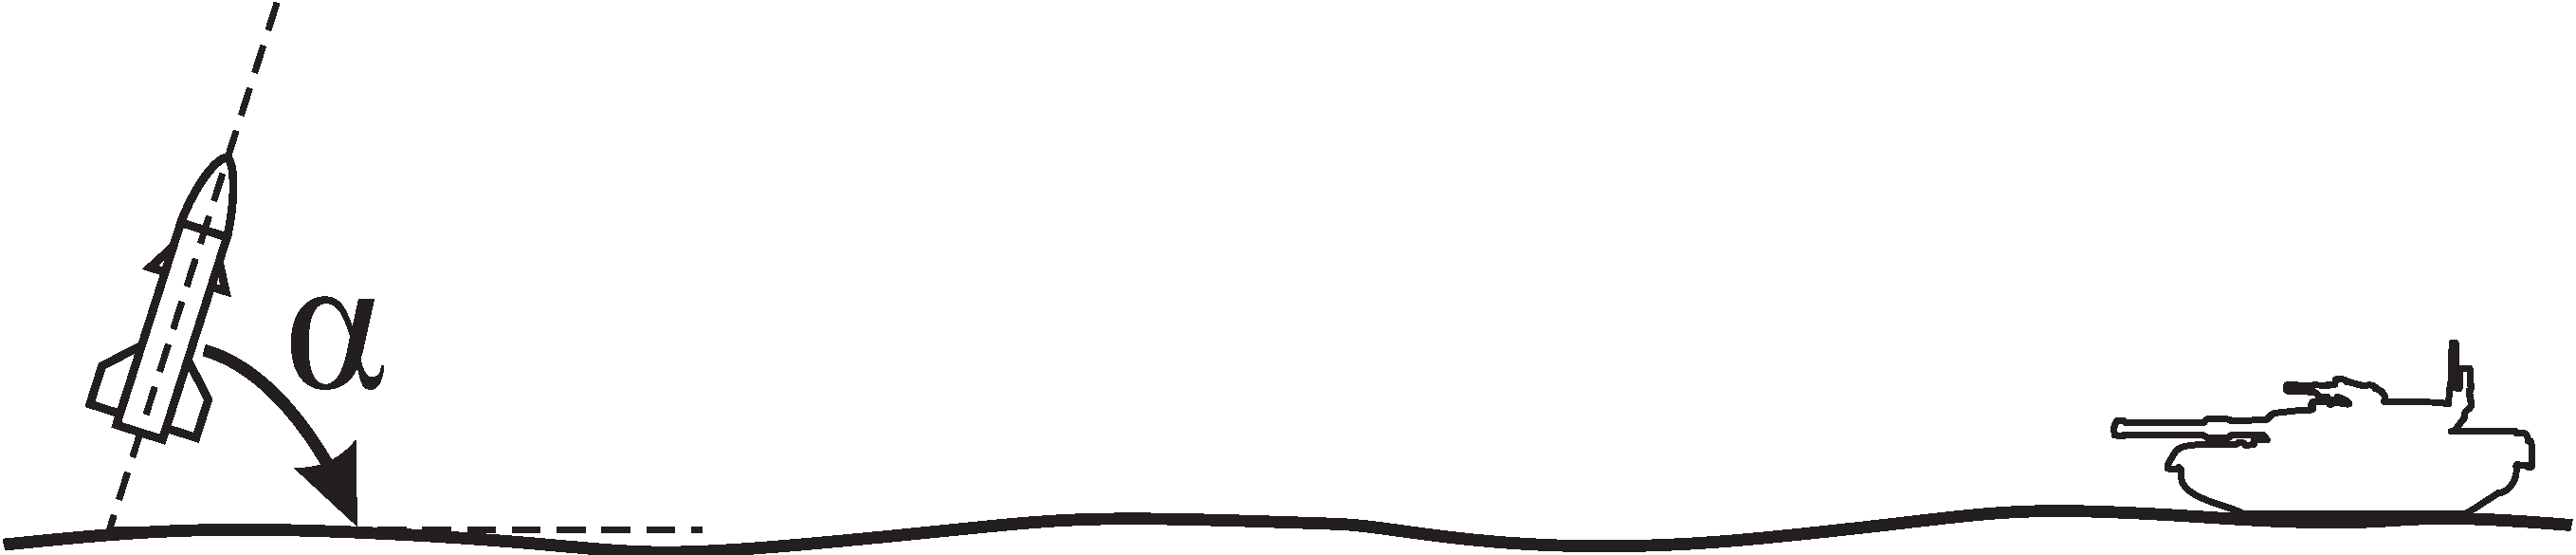
\includegraphics[width=0.475\textwidth]{rys05/alfa1}}}}  \caption{Wyznaczanie trajektorii lotu rakiety: 
	\end{tabular}
  \caption{Średnie czasy odpowiedzi na żądanie względem liczby procesów generujących oraz systemu bazodanowego}
  \label{fig:response-mtc-1}
\end{figure}

Dla tego właśnie przedziału, jedyną zauważalną anomalię dotyczącą zmiany wydajności dostrzec można w kontekście interfejsu programowania aplikacji C\# .NET korzystającego z silnika bazy danych PostgreSQL. W tym przypadku znaczące różnice pomiędzy wydajnością omawianego systemu, a efektywnością drugiego najgorszego rozwiązania odnotowano już dla około \textbf{720} współbieżnie pracujących wątków. Dla tej właśnie metryki, omawiana różnica wynosi \textbf{374 ms}. Wraz ze wzrostem liczby użytkowników o tysiąc, zauważyć możemy różnicę \textbf{759 ms}, a o dwa tysiące - \textbf{2326 ms}. W momencie zaprzestania obserwacji tendencji nieznacznych dysproporcji pomiędzy systemami baz danych (moment ten możemy aproksymować do chwili działania 3750 jednoczesnych procesów-generatorów) dywergencja czasów odpowiedzi osiągnęła wartość \textbf{4855 ms}.

Dysproporcje wskazujące na niezaprzeczalną wyższość określonych rozwiązań nad pozostałymi dostrzegalne są dla rezultatów otrzymywanych w wyniku wspólnej pracy więcej niż czterech tysięcy procesów oprogramowania Apache JMeter. 

Odwołując się do interfejsu zaimplementowanego w technologii NodeJS, zauważyć możemy fakt, że spośród rozwiązań relacyjnych, najniższy skok wartości odnotowały rozwiązania MySQL oraz PostgreSQL. Ponadto, skok ten nastąpił zdecydowanie później, niż miało to miejsce w przypadku pozostałych rozwiązań. Wartym odnotowania są wyniki zaobserwowane dla nierelacyjnego systemu bazodanowego. W przypadku silnika bazy danych MongoDB, średnie czasy odpowiedzi były względnie niskie nie tylko do chwili uruchomienia czterech tysięcy wątków, ale również po tym czasie nie odnotowano gwałtownego wzrostu monitorowanej metryki. W momencie generowania maksymalnego natężenia ruchu sieciowego, zmierzony średni czas odpowiedzi wyniósł \textbf{5846 ms}.

W przypadku rozwiązania zdefiniowanego na bazie technologii Microsoft, zauważalna jest bardzo niska wydajność obsługi komunikacji z rozwiązaniem SQLite (maksymalna zmierzona wartość to \textbf{22515 ms}). Ponadto, silnik bazy danych PostgreSQL, analogicznie do obszaru niższego natężenia ruchu, notuje wyniki gorsze od swoich relacyjnych oraz nierelacyjnych odpowiedników w granicach od \textbf{2111 ms} do \textbf{5373 ms}.

W kontekście pobierania pojedynczego wyniku, wzrosty wartości średniego czasu odpowiedzi posiadają charakterystkę przybliżoną do charakterystyki liniowej. Wyjątkami są tutaj systemy bazy danych MongoDB dla interfejsu napisanego w języku C\#, oraz silnik MySQL dla NodeJS API. W obu przypadkach pojawiają się gwałtowne wzrosty wartości czasu odpowiedzi. Odnosząc się do MongoDB zaobserwować możemy zmianę metryki wydajności od \textbf{1549 ms} do \textbf{5945 ms} na przestrzeni przyrostu wątków od liczby \textbf{3748} do \textbf{4253}. Zmiana ta, utrzymuje się do końca przeprowadzania testu. Dla interfejsu programowania aplikacji uruchamianego w środowisku NodeJS, oraz dla systemu bazodanowego MySQL, anomalia dostrzegana jest dla \textbf{2465} wątków a jej amplituda to \textbf{6721 ms}. Co ciekawe, przekraczając poziom natężenia wynoszący \textbf{2890} wątków, średni czas odpowiedzi zaczyna spadać, aby w punkcie \textbf{4080} stanowić minimum w odniesieniu do pozostałych systemów baz danych.

Poddając pod analizę procedurę zapisu danych do bazy, zgromadzone wyniki wykazują przewagę rozwiązania opartego o język C\#, niezależnie od systemu bazodanowego. Ponadto, liniowa charakterystyka wzrostu metryk dla interfejsu JavaScript zakłócona została pojawieniem się nagłych spadków wydajnościowych. Analogicznie do punktu końcowego pobierania listy obiektów, najmniej znaczący spadek odnotować należy w odniesieniu do nierelacyjnego systemu MongoDB. W tym przypadku zmiana nastąpiła od wartości \textbf{5261 ms} dla \textbf{4247} wątków do wartości \textbf{6203 ms} dla \textbf{5000} wątków.
    
W aspekcie dwóch ostatnich procedur realizowanych przez punkty końcowe interfejsów programowania aplikacji, podobnie jak w przypadku funkcjonalności pozyskiwania pojedynczej encji, zaobserwować możemy przybliżone do liniowych, zmiany monitorowanego parametru wydajności. Spośród interesujących anomalii zaobserwowanych w ramach czterech ostatnich wykresów wyróżnić należy spadek wydajnościowy silnika bazodanowego SQLite w przypadku modyfikacji encji za pomocą interfejsu API .NET. Spadek ten, identyfikowany jest poprzez wzrost średniego czasu odpowiedzi o \textbf{8018 ms}, w przedziale czasowym w którym uruchomiono dodatkowe \textbf{847} wątków. Niestandardowym zachowaniem cechują się również systemy bazodanowe SQL Server oraz MySQL w odniesieniu do operacji usuwania pojedynczego rekordu poprzez API implementowane w języku C\#. Interfejsy korzystające z obu mechanizmów przechowywania danych, do momentu osiągnięcia odpowiednio \textbf{1725} oraz \textbf{1955} współbieżnie pracujących wątków generowania żądań, cechowały się wyjątkowo niskim średnim czasem odpowiedzi (tj. odpowiednio \textbf{827 ms} oraz \textbf{922 ms}).

Podsumowując, zarówno wskazanie wyższości jednej z technologii niezależnie od systemów baz danych, jak i wyróżnienie pojedynczego systemu bazy danych w kontekście realizowanej operacji nie jest możliwe biorąc pod uwagę kształt przeprowadzonego badania. Możliwym jest jednak zaobserowanie niskiego poziomu kompatybilności pomiędzy interfejsem API napisanym w języku C\# oraz systemem baz danych SQLite. Ponadto, relatywnie wysoką wydajnością względem innych rozwiązań bazodanowych cechuje się system nierelacyjny MongoDB. W pięciu na dziesięć porównaniach wydajnościowych, przedstawionych na omawianych wykresach, to właśnie ten silnik baz danych najdłużej utrzymuje najniższą wartość średniego czasu odpowiedzi względem pozostałych rozwiązań.

Przedstawione powyżej wyniki nie dostarczają jednakże pełnego obrazu faktycznej wydajności ewaluowanych usług. Należy pamiętać, że uzyskana odpowiedź na żądanie nie musi być zawsze pozytywna, przez co nie zawsze niesie ona ze sobą informacje pożądaną dla klienta. Na wykresach \ref{fig:response-with-errors} a) oraz \ref{fig:response-with-errors} b) zestawiono ze sobą informacje o średnim czasie odpowiedzi na żądanie, a także o procencie żądań zakończonych niepomyślnie. Poprzez niepomyślne zakończenie żądania, rozumiano zarówno uzyskanie odpowiedzi o niepoprawnym kodzie i treści ciała, jak i zgłoszenie wyjątku protokołu hipertekstowego związanego z odmową aplikacji względem realizacji zapytania. Choć zobrazowano tu tylko i wyłącznie przypadek pojedynczej operacji oraz jednego systemu bazodanowego, analogiczne zachowanie zaobserwować można dla wszystkich pozostałych operacji i jest ono specyficzne dla interfejsu programowania aplikacji. 

\begin{figure}[htb]
    \centering
      \begin{tabular}{@{}ll@{}}
      a) & b) \\
      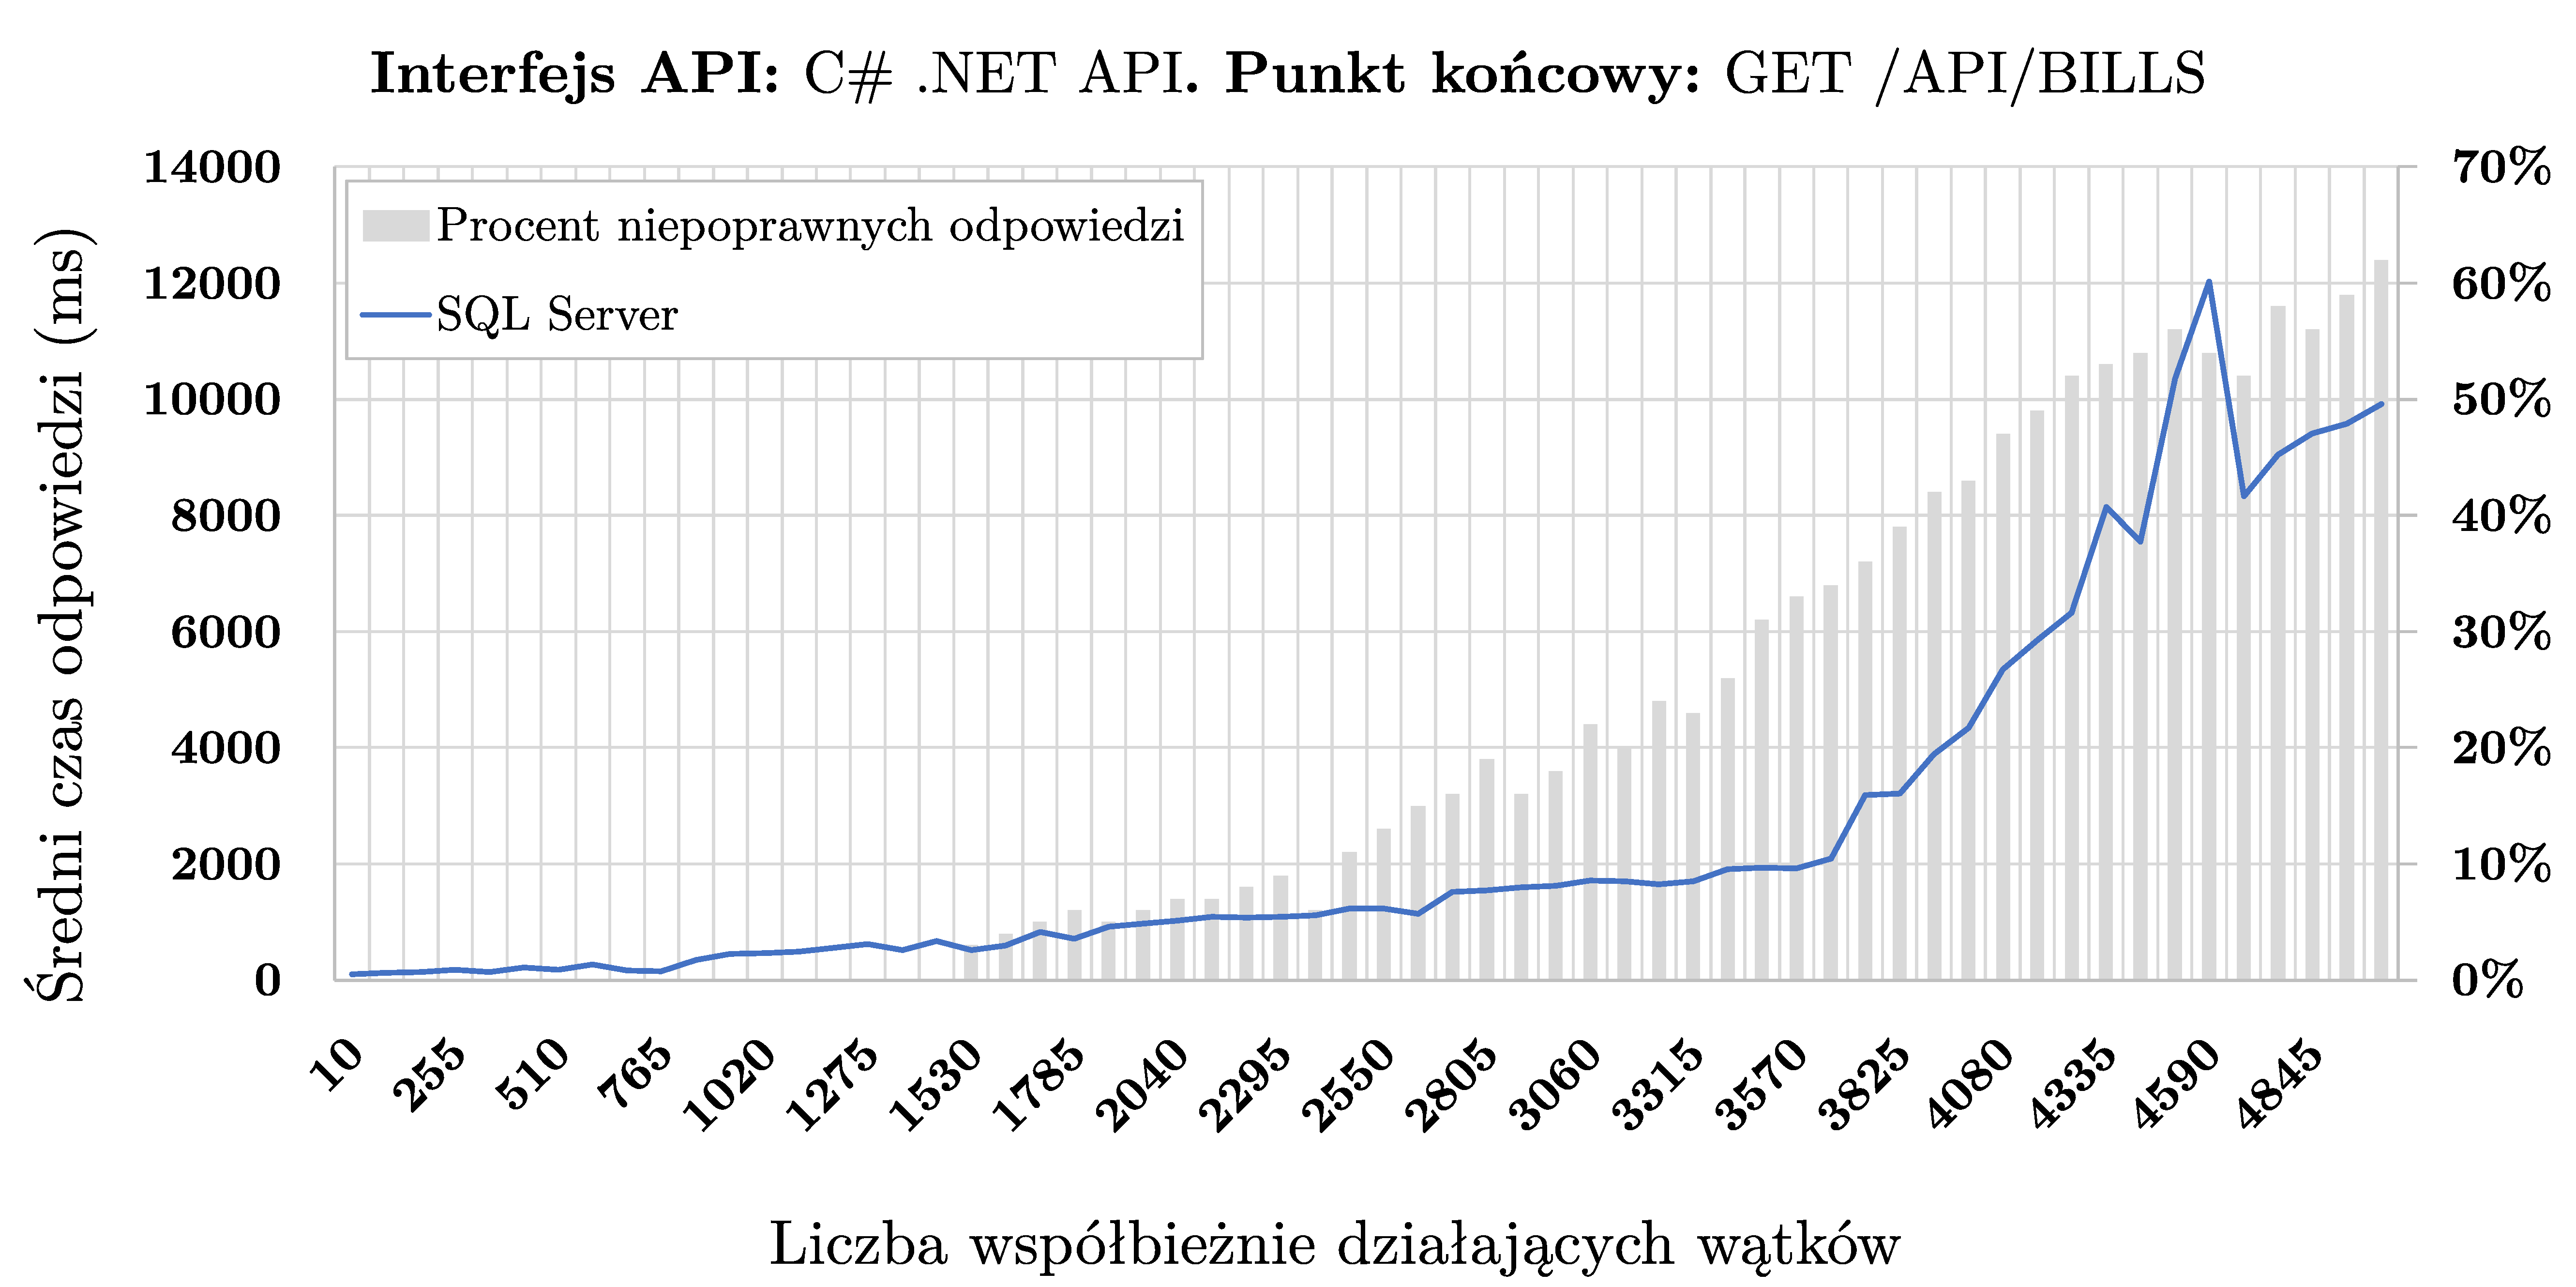
\includegraphics[width=0.49\textwidth]{rys05/response-and-errors-dotnet.pdf} & 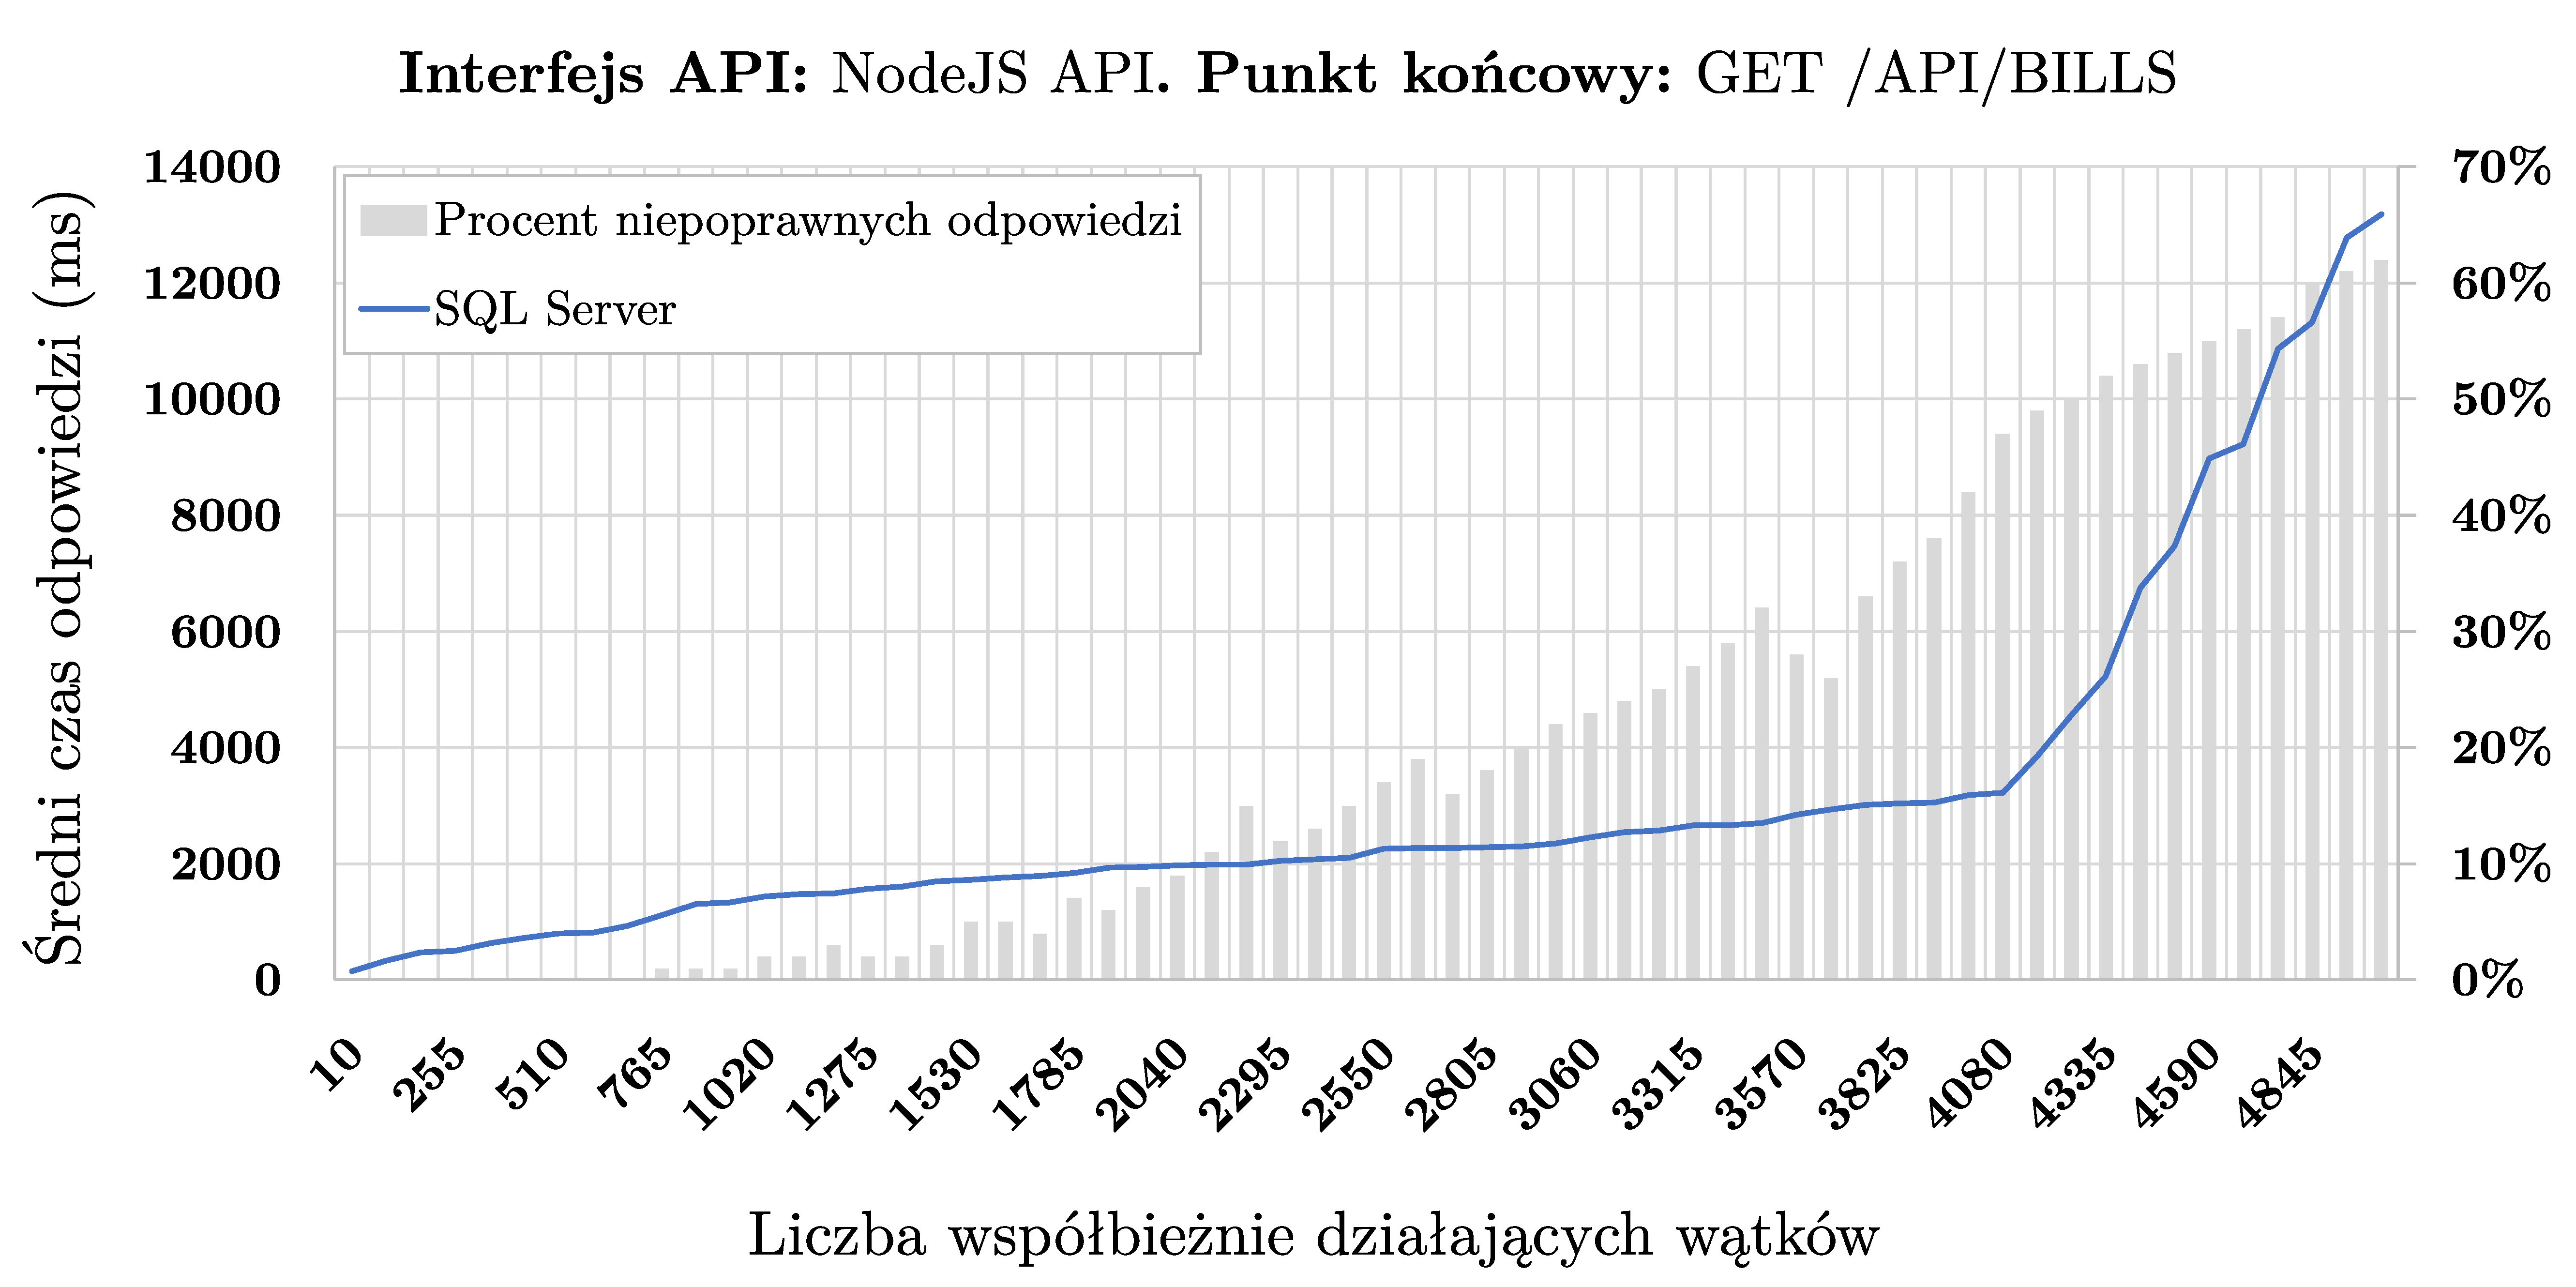
\includegraphics[width=0.49\textwidth]{rys05/response-and-errors-nodejs.pdf}
      % jezeli obraki sa rownej wysokosci, mozna je wyrownac do gory stosujac vtop jak nizej
      % \vtop{\vskip-2ex\hbox{{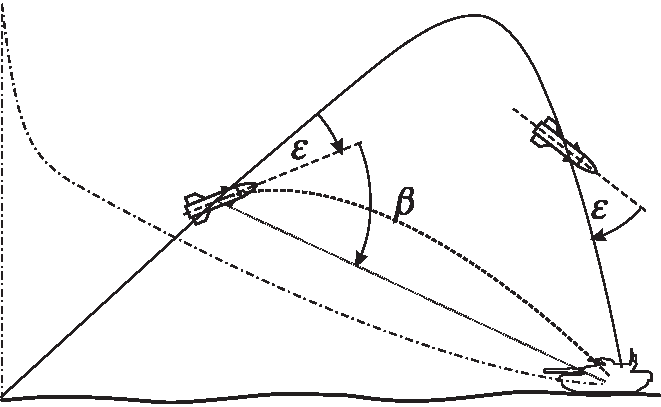
\includegraphics[width=0.475\textwidth]{rys05/beta1}}}} &
      % \vtop{\vskip-2ex\hbox{{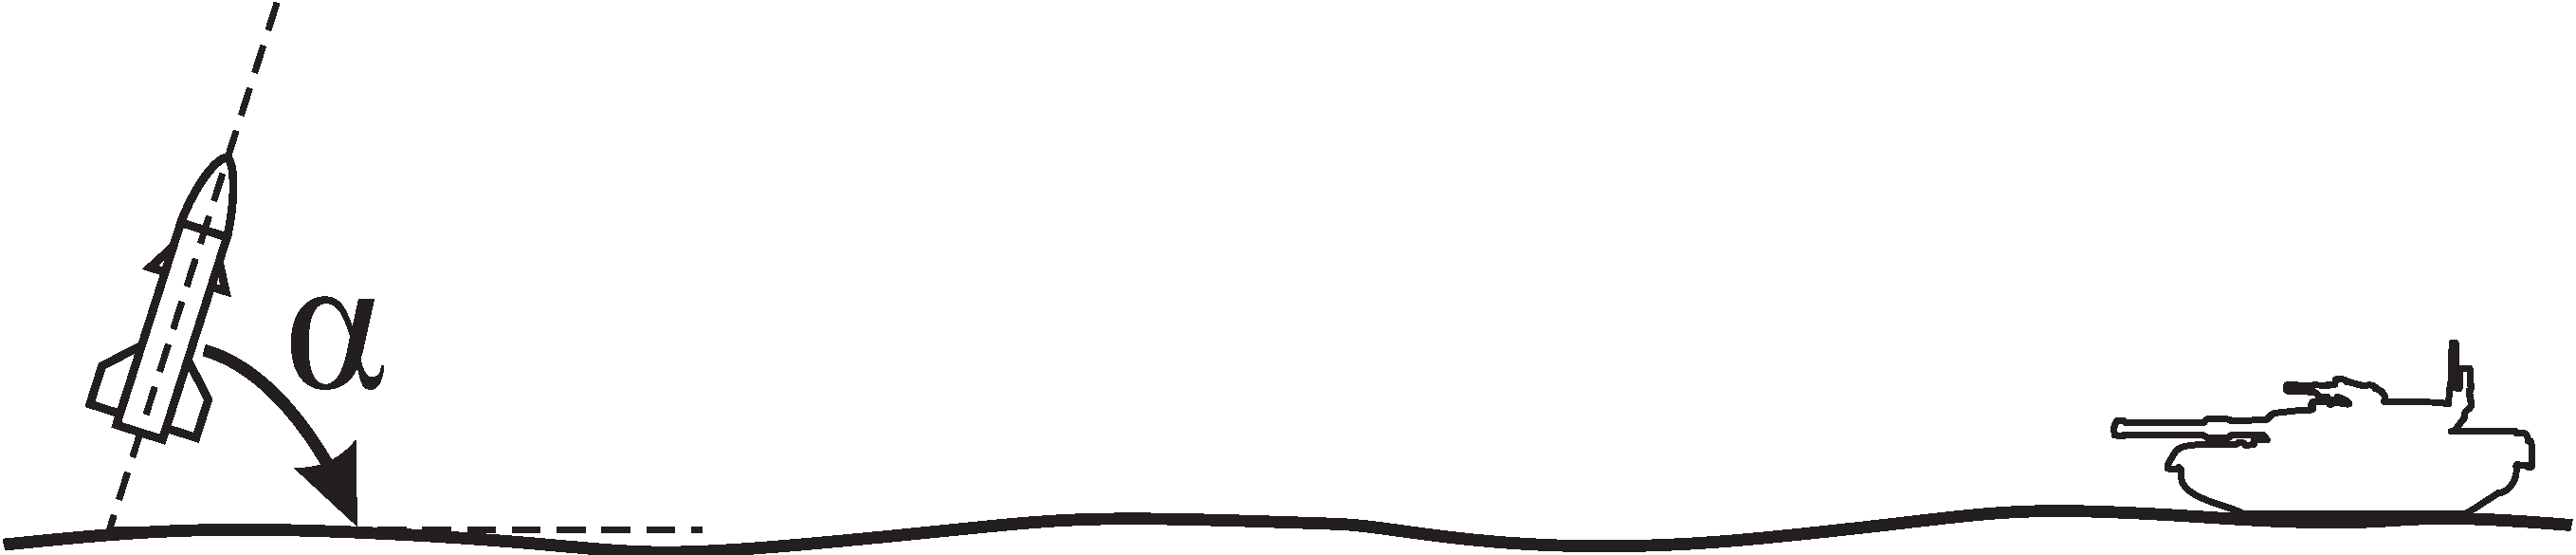
\includegraphics[width=0.475\textwidth]{rys05/alfa1}}}}  \caption{Wyznaczanie trajektorii lotu rakiety: 
      \end{tabular}
    \caption{Średnie czasy odpowiedzi na żądanie oraz procent niepoprawnych odpowiedzi względem liczby procesów generujących}
    \label{fig:response-with-errors}
  \end{figure}

Analizując przedstawione wykresy należy zwrócić uwagę zarówno na moment pojawiania się błędów obsługi żądania, jak i na stopień korelacji błędów z czasem przetwarzania zapytania. W przypadku interfejsu API opartego o technologię .NET widzimy, że procent błędów jest silnie powiązany ze zwiększającym się przedziałem czasowym obsługi komendy, a także intensyfikacją ruchu sieciowego. Oznacza to, że serwer w momencie kolejkowania żądań do przetworzenia, nie bierze pod uwagę ich liczby i stara się przetwarzać każde, jakie do niego dotrze. W związku z odmową realizacji funkcjonalności ze strony API, serwer zgłasza wyjątek protokołu hipertekstowego. Z racji konieczności wykonania pracy w kontekście każdego żądania, niezależnie od niewielkiego prawdopodobieństwa jego pomyślnej realizacji, wydłuża się czas uzyskania odpowiedzi na zapytanie klienckie.

Odnosząc się do interfejsu zaimplementowanego w technologii NodeJS, zaobserwować możemy odmienne zachowanie. Pierwszym aspektem na jaki należy zwrócić uwagę jest pojawienie się błędów obsługi żądania zdecydowanie wcześniej (tj. przy znacząco mniejszej liczbie uruchomionych wątków testowych). Oznacza to, że usługa nie jest w stanie radzić sobie na tyle dobrze z dostarczanym ruchem, jak robi to interfejs napisany w języku C\#. Jednakże, wraz z rosnącym błędem procentowym nie zmienia się czas obsługi żądania. Oznacza to, że komponent serwerowy w ramach API nie przetwarza każdego z zapytań jakie zostanie do niego dostarczone, a także to, że w pewien specyficzny względem swojej charakterystyki sposób, API dokonuje wyboru tych spośród otrzymanych żądań, które mają zostać natychmiastowo odrzucone. Taki model przetwarzania komunikatów pozwala na utrzymanie niskiego poziomu czasu odpowiedzi, jednakże należy wziąć pod uwagę fakt, że nie musi być ona jednoznaczna z poziomem wydajności działania API.
\section{Wpływ zastosowanej technologii na wydajność realizacji operacji współbieżnych}
Niniejsze badanie, przeprowadzone zostało w celu zaobserwowania różnic dotyczących sposobu przetwarzania długo trwających operacji. Potencjalnie różnice te, związane mogą być z odmienną implementacją wewnętrznych mechanizmów przetwarzania współbieżnego, a także diametralnie innym podejściem obu technologii do zagadnienia wielowątkowości. Zdecydowano się na implementację algorytmu rozwiązującego symetryczny problem komiwojażera, bazującego na metaheurystyce genetycznej. Elementy charakterystyczne względem omawianego rozwiązania przedstawiono w sekcji \ref{label:algorytm-genetyczny}. Napisane programy, zawarte są wewnątrz warstwy logiki biznesowej interfejsów API, a punktem wprowadzania danych dla algorytmów są określone punkty końcowe. W odniesieniu do przekazywanych danych wejściowych, wyróżnić należy ciało żądania, zawierające tablicę obiektów notacji JSON. Obiekty te, identyfikują określone lokalizacje poprzez wprowadzenie parametrów długości oraz szerokości geograficznej. Ponadto, przekazywany zostaje parametr czasu trwania głównej pętli algorytmu (tj. jak długo program powinien dokonywać kalkulacji), a także wartość wyniku optymalnego, względem której program powinien porównać uzyskany rezultat.

Odnosząc się do protokołu badawczego, zdecydowano się na wykonanie pomiarów jakości uzyskanego rozwiązania, a także liczby iteracji głównej pętli implementowanego algorytmu. Metryki te, zostały zebrane w kontekście uruchomienia programu dla pietnastu odmiennych zbiorów danych testowych, dostępnych w ramach otwartej biblioteki TSPLib \cite{TSPLIB_ARTICLE}. Dla każdego ze zbiorów danych, trzydziestokrotnie powtórzono wywołanie algorytmu, w obrębie każdego z czterech różnych czasów wykonywania iteracji głównej programu. Czasy te to: 15s, 30s, 45s oraz 60s. W momencie przeprowadzenia badania, a także przez cały okres jego trwania, uruchomionych było 30 współbieżnie pracujących wątków będących generatorami żądań.

Przed rozpoczęciem realizacji omówionego protokołu przeprowadzono ewaluację funkcjonalną, stanowiącą warunek początkowy podjęcia badań. Ewaluacja ta, polegała na pięciokrotnym odwołaniu się punktów końcowych api obu technologii, wprowadzając jako dane wejściowe, zbiory współrzędnych dostępnych w ramach biblioteki TSPLib. Warto zaznaczyć, że są to zbiory inne, niż te wykorzystane następnie w faktycznym badaniu. Kryterium akceptacji warunku początkowego, było pomyślne wykonanie algorytmu w każdym ze zdefiniowanych przypadków funkcjonalnych, a także zwrócenie poprawnej odpowiedzi w czasie zgodnym z parametrem czasu wykonania alogytmu. Oba wymienione kryteria zostały w czasie ewaluacji funkcjonalnej spełnione.

Następnie, przygotowano lokalną topologię fizyczną nr 2, której schemat zaprezentowany został w sekcji \ref{sec:lokalne-srodowisko-badawcze-ver-2} oraz rozpoczęto generowanie żądań. Już na tym etapie, a jeszcze przed otrzymaniem wyników działania algorytmu, zaobserwowano interesujące zachowanie dotyczące obsługi długo trwających żądań. Analizując czasy rozpoczęcia oraz zakończenia pracy dla poszczególnych wątków Apache JMeter, a także całkowity czas trwania badania dla każdego z interfejsów programowania aplikacji, dostrzeżono pełną sekwencyjność przetwarzania zapytań w przypadku API zaimplementowanego w technologii JavaScript / NodeJS, a także częściowe zrównoleglenie operacji w kontekście technologii C\# .NET. W konsekwencji tego, ewaluacja usługi sieciowej opartej o NodeJS trwała 18 godzin i 52 minuty, podczas gdy badanie interfejsu napisanego w języku programowania C\# -- 5 godzin i 27 minut. Tak znacząca dysproporcja wynika ze sposobu zarządzania wykonaniem zapytań poprzez zastosowanie podejścia wielowątkowości, a także pracy z wykorzystaniem pojedynczego wątku.

Kiedy żądanie zacznie być przetwarzane przez interfejs programowania aplikacji NodeJS, jest ono wykonywane do momentu: uzyskania wyniku, przekroczenia dozwolonego czasu realizacji zapytania \textit{(ang. timeout)}, bądź też przekazania tokenu przerwania \textit{(ang. cancellation token)}. Jeżeli w czasie obsługi żądania pojawi się następne, musi ono zostać przekazane do kolejki, po to, aby stać się aktywnym po zakończeniu przetwarzania poprzedniej wiadomości.

Analizując wewnętrzne mechanizmy usługi sieciowej implementowanej w języku C\# zauważyć możemy odmienne, niż zaprezentowane powyżej podejście. W związku z faktem utworzenia nowego wątku dla głównej pętli algorytmu, wątek podstawowy programu nie jest obciążony koniecznością realizacji jakichkolwiek dodatkowych operacji i oczekuje na uzyskanie wyników z procesu potomnego. Jeżeli w czasie oczekiwania pojawi się przychodzące żądanie, wątek główny zapisuje kontekst wywołania dla obecnego zapytania, przechodzi do realizacji kolejnego z nich, a po jego zakończeniu, bądź w momencie wyczekiwania na zakończenie, przełącza się do kontekstu poprzedniego zadania, aby zweryfikować jego status. Dzięki zastosowaniu takiego podejścia, które możliwe jest tylko w sytuacji dostępności wielu wątków w ramach pojedynczego programu, usługa sieciowa nie jest blokowana względem innych klientów.

Po ukończeniu obsługi wszystkich wygenerowanych żądań, przez oba systemy internetowe, uśredniono serie każdych 30 rezultatów, uzyskanych względem różnych zbiorów testowych oraz odmiennych czasów wykonania. Opracowane wyniki, przedstawiono w tabelach \ref{tab:mtc-2} oraz \ref{tab:mtc-2-2}.

\begin{table}[ht]
  \centering
  \caption{Wydajność realizacji algorytmu genetycznego dla problemu komiwojażera w zależności od czasu przetwarzania oraz technologii -- współczynnik jakości rozwiązania}
  \label{tab:mtc-2}
  \resizebox{\columnwidth}{!}{%
  \begin{tabular}{|l|llll|llll|}
  \hline
  \multicolumn{1}{|c|}{\multirow{2}{*}{}} &
    \multicolumn{4}{c|}{C\# / .NET} &
    \multicolumn{4}{c|}{JavaScript / NodeJS} \\ \cline{2-9} 
  \multicolumn{1}{|c|}{} &
    \multicolumn{1}{c|}{15s} &
    \multicolumn{1}{c|}{30s} &
    \multicolumn{1}{c|}{45s} &
    \multicolumn{1}{c|}{60s} &
    \multicolumn{1}{c|}{15s} &
    \multicolumn{1}{c|}{30s} &
    \multicolumn{1}{c|}{45s} &
    \multicolumn{1}{c|}{60s} \\ \hline\hline
  burma14 &
    \multicolumn{1}{l|}{0,3462 } &
    \multicolumn{1}{l|}{\textbf{0,6847}} &
    \multicolumn{1}{l|}{0,8475 } &
    \textbf{0,8589} &
    \multicolumn{1}{l|}{0,2983 } &
    \multicolumn{1}{l|}{\textbf{0,5943}} &
    \multicolumn{1}{l|}{0,7636 } &
    0,7579  \\ \hline
  ulysses16 &
    \multicolumn{1}{l|}{0,5299} &
    \multicolumn{1}{l|}{0,3910 } &
    \multicolumn{1}{l|}{0,9270 } &
    0,6549  &
    \multicolumn{1}{l|}{0,4817 } &
    \multicolumn{1}{l|}{0,2857 } &
    \multicolumn{1}{l|}{0,8297 } &
    0,5354  \\ \hline
  ulysses22 &
    \multicolumn{1}{l|}{0,5271 } &
    \multicolumn{1}{l|}{0,4171 } &
    \multicolumn{1}{l|}{0,9312 } &
    0,7824  &
    \multicolumn{1}{l|}{\textbf{0,5488} } &
    \multicolumn{1}{l|}{0,4668 } &
    \multicolumn{1}{l|}{0,8728 } &
    0,6717  \\ \hline
  att48 &
    \multicolumn{1}{l|}{0,0493 } &
    \multicolumn{1}{l|}{0,0611 } &
    \multicolumn{1}{l|}{0,3129 } &
    0,2623  &
    \multicolumn{1}{l|}{0,0242 } &
    \multicolumn{1}{l|}{0,0238 } &
    \multicolumn{1}{l|}{0,2413 } &
    0,2903  \\ \hline
  berlin52 &
    \multicolumn{1}{l|}{0,2316 } &
    \multicolumn{1}{l|}{0,2484 } &
    \multicolumn{1}{l|}{\textbf{0,9718}} &
    0,8398  &
    \multicolumn{1}{l|}{0,2239 } &
    \multicolumn{1}{l|}{0,3861 } &
    \multicolumn{1}{l|}{\textbf{0,9202} } &
    0,7642  \\ \hline
  gr96 &
    \multicolumn{1}{l|}{0,4798 } &
    \multicolumn{1}{l|}{0,1617 } &
    \multicolumn{1}{l|}{0,9274 } &
    0,7808  &
    \multicolumn{1}{l|}{0,4874 } &
    \multicolumn{1}{l|}{0,1386 } &
    \multicolumn{1}{l|}{0,8606 } &
    0,7103  \\ \hline
  bier127 &
    \multicolumn{1}{l|}{0,2313 } &
    \multicolumn{1}{l|}{0,1963 } &
    \multicolumn{1}{l|}{0,8473 } &
    0,8505  &
    \multicolumn{1}{l|}{0,1162 } &
    \multicolumn{1}{l|}{0,1928 } &
    \multicolumn{1}{l|}{0,7906 } &
    0,7792  \\ \hline
  ch130 &
    \multicolumn{1}{l|}{0,0947 } &
    \multicolumn{1}{l|}{0,1328 } &
    \multicolumn{1}{l|}{0,8072 } &
    0,8066  &
    \multicolumn{1}{l|}{0,0575 } &
    \multicolumn{1}{l|}{0,1457 } &
    \multicolumn{1}{l|}{0,7521 } &
    0,6828  \\ \hline
  ch150 &
    \multicolumn{1}{l|}{0,0784 } &
    \multicolumn{1}{l|}{0,1140 } &
    \multicolumn{1}{l|}{0,8584 } &
    0,7966  &
    \multicolumn{1}{l|}{0,0812 } &
    \multicolumn{1}{l|}{0,1483 } &
    \multicolumn{1}{l|}{0,7900 } &
    \textbf{0,7991 } \\ \hline
  tsp225 &
    \multicolumn{1}{l|}{0,2819 } &
    \multicolumn{1}{l|}{0,0988 } &
    \multicolumn{1}{l|}{0,7801 } &
    0,8311  &
    \multicolumn{1}{l|}{0,3057 } &
    \multicolumn{1}{l|}{0,0826 } &
    \multicolumn{1}{l|}{0,8209 } &
    0,7533  \\ \hline
  att532 &
    \multicolumn{1}{l|}{0,0194 } &
    \multicolumn{1}{l|}{0,0171 } &
    \multicolumn{1}{l|}{0,2226 } &
    0,2470  &
    \multicolumn{1}{l|}{0,0116 } &
    \multicolumn{1}{l|}{0,0233 } &
    \multicolumn{1}{l|}{0,2650 } &
    0,1498  \\ \hline
  u574 &
    \multicolumn{1}{l|}{\textbf{0,5940}} &
    \multicolumn{1}{l|}{0,5454 } &
    \multicolumn{1}{l|}{0,6460 } &
    0,7872  &
    \multicolumn{1}{l|}{0,4821 } &
    \multicolumn{1}{l|}{0,3782 } &
    \multicolumn{1}{l|}{0,5836 } &
    0,6573  \\ \hline
  u724 &
    \multicolumn{1}{l|}{0,1620 } &
    \multicolumn{1}{l|}{0,0483 } &
    \multicolumn{1}{l|}{0,6529 } &
    0,7718  &
    \multicolumn{1}{l|}{0,0943 } &
    \multicolumn{1}{l|}{0,0472 } &
    \multicolumn{1}{l|}{0,5747 } &
    0,6369  \\ \hline
  vm1084 &
    \multicolumn{1}{l|}{0,0289 } &
    \multicolumn{1}{l|}{0,0273 } &
    \multicolumn{1}{l|}{0,5971 } &
    0,7938  &
    \multicolumn{1}{l|}{0,0051 } &
    \multicolumn{1}{l|}{0,0381 } &
    \multicolumn{1}{l|}{0,5126 } &
    0,7962  \\ \hline
  d1291 &
    \multicolumn{1}{l|}{0,1927 } &
    \multicolumn{1}{l|}{0,2930 } &
    \multicolumn{1}{l|}{0,5711 } &
    0,8421  &
    \multicolumn{1}{l|}{0,1768 } &
    \multicolumn{1}{l|}{0,1016 } &
    \multicolumn{1}{l|}{0,5979 } &
    0,7438  \\ \hline\hline
    \multicolumn{1}{|l|}{\textbf{Średnia ranga}} &
    \multicolumn{1}{l|}{3,0000} &
    \multicolumn{1}{l|}{2,6667} &
    \multicolumn{1}{l|}{7,0667} &
    \multicolumn{1}{l|}{7,0000} &
    \multicolumn{1}{l|}{2,1334} &
    \multicolumn{1}{l|}{2,6667} &
    \multicolumn{1}{l|}{6,0667} &
    \multicolumn{1}{l|}{5,8000} \\ \hline
  \end{tabular}%
  }
\end{table}

\begin{table}[ht]
  \centering
  \caption{Wydajność realizacji algorytmu genetycznego dla problemu komiwojażera w zależności od czasu przetwarzania oraz technologii -- liczba iteracji pętli algorytmu}
  \label{tab:mtc-2-2}
  \resizebox{\columnwidth}{!}{%
  \begin{tabular}{|l|llll|llll|}
  \hline
  \multicolumn{1}{|c|}{\multirow{2}{*}{}} &
    \multicolumn{4}{c|}{C\# / .NET} &
    \multicolumn{4}{c|}{JavaScript / NodeJS} \\ \cline{2-9} 
  \multicolumn{1}{|c|}{} &
    \multicolumn{1}{c|}{15s} &
    \multicolumn{1}{c|}{30s} &
    \multicolumn{1}{c|}{45s} &
    \multicolumn{1}{c|}{60s} &
    \multicolumn{1}{c|}{15s} &
    \multicolumn{1}{c|}{30s} &
    \multicolumn{1}{c|}{45s} &
    \multicolumn{1}{c|}{60s} \\ \hline\hline
  burma14 &
    \multicolumn{1}{l|}{71725} &
    \multicolumn{1}{l|}{130514} &
    \multicolumn{1}{l|}{201224} &
    \multicolumn{1}{l|}{\textbf{248972}} &
    \multicolumn{1}{l|}{71747} &
    \multicolumn{1}{l|}{129134} &
    \multicolumn{1}{l|}{\textbf{205306}} &
    227232 \\ \hline
  ulysses16 &
    \multicolumn{1}{l|}{68491} &
    \multicolumn{1}{l|}{124929} &
    \multicolumn{1}{l|}{174385} &
    244773 &
    \multicolumn{1}{l|}{68488} &
    \multicolumn{1}{l|}{122619} &
    \multicolumn{1}{l|}{192590} &
    219521 \\ \hline
  ulysses22 &
    \multicolumn{1}{l|}{33520} &
    \multicolumn{1}{l|}{117580} &
    \multicolumn{1}{l|}{164707} &
    224099 &
    \multicolumn{1}{l|}{63802} &
    \multicolumn{1}{l|}{129397} &
    \multicolumn{1}{l|}{176319} &
    203753 \\ \hline
  att48 &
    \multicolumn{1}{l|}{62550} &
    \multicolumn{1}{l|}{120072} &
    \multicolumn{1}{l|}{183853} &
    233205 &
    \multicolumn{1}{l|}{62843} &
    \multicolumn{1}{l|}{134376} &
    \multicolumn{1}{l|}{157470} &
    198158 \\ \hline
  berlin52 &
    \multicolumn{1}{l|}{\textbf{72721}} &
    \multicolumn{1}{l|}{114196} &
    \multicolumn{1}{l|}{190914} &
    235500 &
    \multicolumn{1}{l|}{\textbf{72331}} &
    \multicolumn{1}{l|}{122215} &
    \multicolumn{1}{l|}{182668} &
    237310 \\ \hline
  gr96 &
    \multicolumn{1}{l|}{62745} &
    \multicolumn{1}{l|}{133156} &
    \multicolumn{1}{l|}{172122} &
    203419 &
    \multicolumn{1}{l|}{63117} &
    \multicolumn{1}{l|}{99062} &
    \multicolumn{1}{l|}{162453} &
    204787 \\ \hline
  bier127 &
    \multicolumn{1}{l|}{66491} &
    \multicolumn{1}{l|}{132354} &
    \multicolumn{1}{l|}{179792} &
    247307 &
    \multicolumn{1}{l|}{66123} &
    \multicolumn{1}{l|}{117603} &
    \multicolumn{1}{l|}{188063} &
    227924 \\ \hline
  ch130 &
    \multicolumn{1}{l|}{62713} &
    \multicolumn{1}{l|}{118125} &
    \multicolumn{1}{l|}{174455} &
    234333 &
    \multicolumn{1}{l|}{62785} &
    \multicolumn{1}{l|}{127119} &
    \multicolumn{1}{l|}{159485} &
   223465 \\ \hline
  ch150 &
    \multicolumn{1}{l|}{66845} &
    \multicolumn{1}{l|}{123024} &
    \multicolumn{1}{l|}{179031} &
    235174 &
    \multicolumn{1}{l|}{66984} &
    \multicolumn{1}{l|}{138917} &
    \multicolumn{1}{l|}{185943} &
    211357 \\ \hline
  tsp225 &
    \multicolumn{1}{l|}{61923} &
    \multicolumn{1}{l|}{124816} &
    \multicolumn{1}{l|}{163056} &
    202829 &
    \multicolumn{1}{l|}{61479} &
    \multicolumn{1}{l|}{126286} &
    \multicolumn{1}{l|}{173199} &
    224409 \\ \hline
  att532 &
    \multicolumn{1}{l|}{65333} &
    \multicolumn{1}{l|}{\textbf{153374}} &
    \multicolumn{1}{l|}{188061} &
    220558 &
    \multicolumn{1}{l|}{65372} &
    \multicolumn{1}{l|}{121134} &
    \multicolumn{1}{l|}{173916} &
    240112 \\ \hline
  u574 &
    \multicolumn{1}{l|}{70850} &
    \multicolumn{1}{l|}{133559} &
    \multicolumn{1}{l|}{190742} &
    231134 &
    \multicolumn{1}{l|}{70639} &
    \multicolumn{1}{l|}{106502} &
    \multicolumn{1}{l|}{196297} &
    \textbf{248733} \\ \hline
  u724 &
    \multicolumn{1}{l|}{69793} &
    \multicolumn{1}{l|}{120363} &
    \multicolumn{1}{l|}{\textbf{205031}} &
    226060 &
    \multicolumn{1}{l|}{69700} &
    \multicolumn{1}{l|}{117866} &
    \multicolumn{1}{l|}{200697} &
    229731 \\ \hline
  vm1084 &
    \multicolumn{1}{l|}{64393} &
    \multicolumn{1}{l|}{111650} &
    \multicolumn{1}{l|}{192909} &
    225794 &
    \multicolumn{1}{l|}{64545} &
    \multicolumn{1}{l|}{122070} &
    \multicolumn{1}{l|}{174608} &
    227990 \\ \hline
  d1291 &
    \multicolumn{1}{l|}{68067} &
    \multicolumn{1}{l|}{120889} &
    \multicolumn{1}{l|}{199096} &
    235376 &
    \multicolumn{1}{l|}{67843} &
    \multicolumn{1}{l|}{\textbf{140742}} &
    \multicolumn{1}{l|}{196741} &
    238146 \\ \hline
  \end{tabular}%
  }
\end{table}

Analizując zgromadzone rezultaty, zauważyć należy przewagę interfejsu programowania aplikacji zaimplementowanego w technologii C\# .NET, w kontekście wartości współczynnika jakości rozwiązania. Na 60 uśrednionych wartości tego parametru, interfejs API NodeJS notuje wyniki lepsze zaledwie w 15 przypadkach. Ponadto, zauważyć należy, że niezależnie od technologii, czas wykonywania algorytmu nie zawsze musi przekładać się na uzyskanie lepszego rozwiązania. Niedeterministyczna charakterystyka algorytmu genetycznego jest powodem pojawiania się gorszych rozwiązań, pomimo pracy algorytmu przez dłuższy czas. Odnosząc się do wartości liczby iteracji głównej pętli programu, różnice cechujące się określoną tendencją nie są zauważalne. Wynika to z dwóch następujących faktów. Po pierwsze, kod źródłowy C\#, z chwilą translacji do języka pośredniego \textit{(ang. intermediate language)}, ulega wewnętrznej optymalizacji przeprowadzanej bezpośrednio przez mechanizmy języka. Po drugie, mechanizmy wykorzystywane do przetwarzania list w C\# dostępne w ramach biblioteki LINQ, wprowadzają dodatkowy narzut związany z koniecznością budowy wewnętrznej struktury danych związanej z przetwarzaną listą. Dlatego też, jakikolwiek wzrost efektywności związany ze wspomnianymi w pierwszym fakcie optymalizacjami, może zostać redukowany poprzez spadek wydajnościowy wprowadzany przez instrukcje przetwarzania list. Mechanizmy przetwarzania kolekcji w ramach języka JavaScript z kolei, nie wprowadzają dodatkowego opóźnienia w wykonywaniu kodu, jednakże na etapie interpretacji wydajność implementowanego programu nie ulega zmianie.

Odwołując się do różnic w kontekście opracowywanych kolekcji danych, zauważyć można bardzo słabe rezultaty dla zbiorów \textbf{att48} oraz \textbf{att532}. Uzyskane w tych przypadkach długości najkrótszych tras są niemalże 5 krotnie większe, niż rozwiązania optymalne. Z drugiej strony, zaobserwować możemy rozwiązania znacząco bliskie optymalnym w odniesieniu do zbioru \textbf{gr96} dla interfejsu NodeJS oraz zbioru \textbf{bier127} dla interfejsu C\# .NET.

W celu wykazania istnotnych statystycznie różnic dotyczących rezultatów zgromadzonych dla określonych konfiguracji badania, wykonano parowe testy statystyczne bazujące na teście Wilcoxona. Test ten, jest nieparametryczną odmianą procedury t-Studenta, zakładającą jako hipotezę zerową zgodność wartości środkowych w odpowiadających sobie populacjach. Jako poziom istotności przyjęto wartość 0,05. Na podstawie tego właśnie testu, wyliczono średnie rangi dla poszczególnych czasów wykonania algorytmów w kontekście wartości współczynnika uzyskanego rezultatu do rozwiązania optymalnego.

Analizując przeprowadzoną ewaluację statystyczną, wykazać należy istotną wyższość rozwiązań uzyskanych przez interfejs programowania aplikacji języka C\# w kontekście czasów wykonania równych 45s oraz 60s. W pozostałych przypadkach różnice nie są istotne statystycznie przy uwzględnieniu poziomu istotności 0,05. Macierz istotności statystycznej przedstawiono w tabeli \ref{tab:stat-mtc2}.

\begin{table}[htb]
  \centering
  \caption{Macierz istotności statystycznej dla współczynników jakości rozwiązania pozyskanych w ramach badania wydajności obsługi operacji współbieżnych}
  \label{tab:stat-mtc2}
  \resizebox{\columnwidth}{!}{%
  \begin{tabular}{|c|c|c|c|c|c|c|c|c|}
  \hline
   &
    \textbf{15s (C\#)} &
    \textbf{30s (C\#)} &
    \textbf{45s (C\#)} &
    \textbf{60s (C\#)} &
    \textbf{15s (NodeJS)} &
    \textbf{30s (NodeJS)} &
    \textbf{45s (NodeJS)} &
    \textbf{60s (NodeJS)} \\ \hline\hline
  \textbf{15s (C\#)}    & 0 & 0 & 0 & 0 & 0 & 0 & 0 & 0 \\ \hline
  \textbf{30s (C\#)}    & 1 & 0 & 0 & 0 & 1 & 0 & 0 & 0 \\ \hline
  \textbf{45s (C\#)}    & 1 & 1 & 0 & 0 & 1 & 1 & 1 & 0 \\ \hline
  \textbf{60s (C\#)}    & 1 & 1 & 1 & 0 & 1 & 1 & 1 & 1 \\ \hline
  \textbf{15s (NodeJS)} & 0 & 0 & 0 & 0 & 0 & 0 & 0 & 0 \\ \hline
  \textbf{30s (NodeJS)} & 0 & 0 & 0 & 0 & 1 & 0 & 0 & 0 \\ \hline
  \textbf{45s (NodeJS)} & 1 & 1 & 0 & 0 & 1 & 1 & 0 & 0 \\ \hline
  \textbf{60s (NodeJS)} & 1 & 1 & 0 & 0 & 1 & 1 & 0 & 0 \\ \hline
  \end{tabular}%
  }
  \end{table}

\section{Wpływ zastosowanej technologii na efektywność obsługi operacji asynchronicznych}
W ramach omawianego badania dokonano analizy wydajności realizacji operacji asynchronicznych względem technologii wykorzystywanych do implementacji porównywanych interfejsów programowania aplikacji. Operacje te, znajdują szerokie zastosowanie wewnątrz kodu źródłowego usług sieciowych, będąc wykorzystywanym w celu uzyskania dostępu i zarządzania plikami, odwoływania się do zewnętrznych źródeł danych, czy też synchronizowania egzekucji wybranych fragmentów kodu programu w czasie.

Zrealizowany eksperyment polegał na obserwacji czasów wykonań operacji asynchronicznych, względem zmiennej liczby encji pobieranych za ich pomocą. Elementy modelu danych, pozyskiwane były poprzez generowanie żądań protokołu hipertekstowego w kierunku zewnętrznej usługi sieciowej. Usługa ta, znajdowała się wewnątrz sieci lokalnej i została zaimplementowana intencjonalnie na potrzeby tego badania. Interfejs programowania aplikacji poddawany ocenie, korzystając z natywnego klienta protokołu hipertekstowego, wykonuje 30 iteracji, w ramach których pozyskuje kolejno 100, 200, 500, 1000, 2000, oraz 5000 encji bazodanowych. Dla każdej z wykonywanych operacji, odnotowany zostaje czas jej ukończenia, a także binarna wartość wskazująca na jej poprawność. W badaniu wykorzystano topologię fizyczną nr 3 przedstawioną w sekcji \ref{sec:lokalne-srodowisko-badawcze-ver-3}, a także wariant pierwszy planu testowego nr 2 omówiony w punkcie \ref{plan-testowy-2-wariant-1}. Wiąże się to z uruchomieniem grupy stu wątków w przedziale czasowym dziesięciu minut.

Pozyskane w ramach badania rezultaty uśredniono, a następnie zaprezentowano na wykresie \ref{fig:async-times}. Zdecydowano się nie uwzględniać metryki procentowego błędu związanego z niepoprawnym wykonaniem żądań, ponieważ niezależnie od poddawanego analizie przypadku, był on równy zero.

\begin{figure}[H]
  \centering
   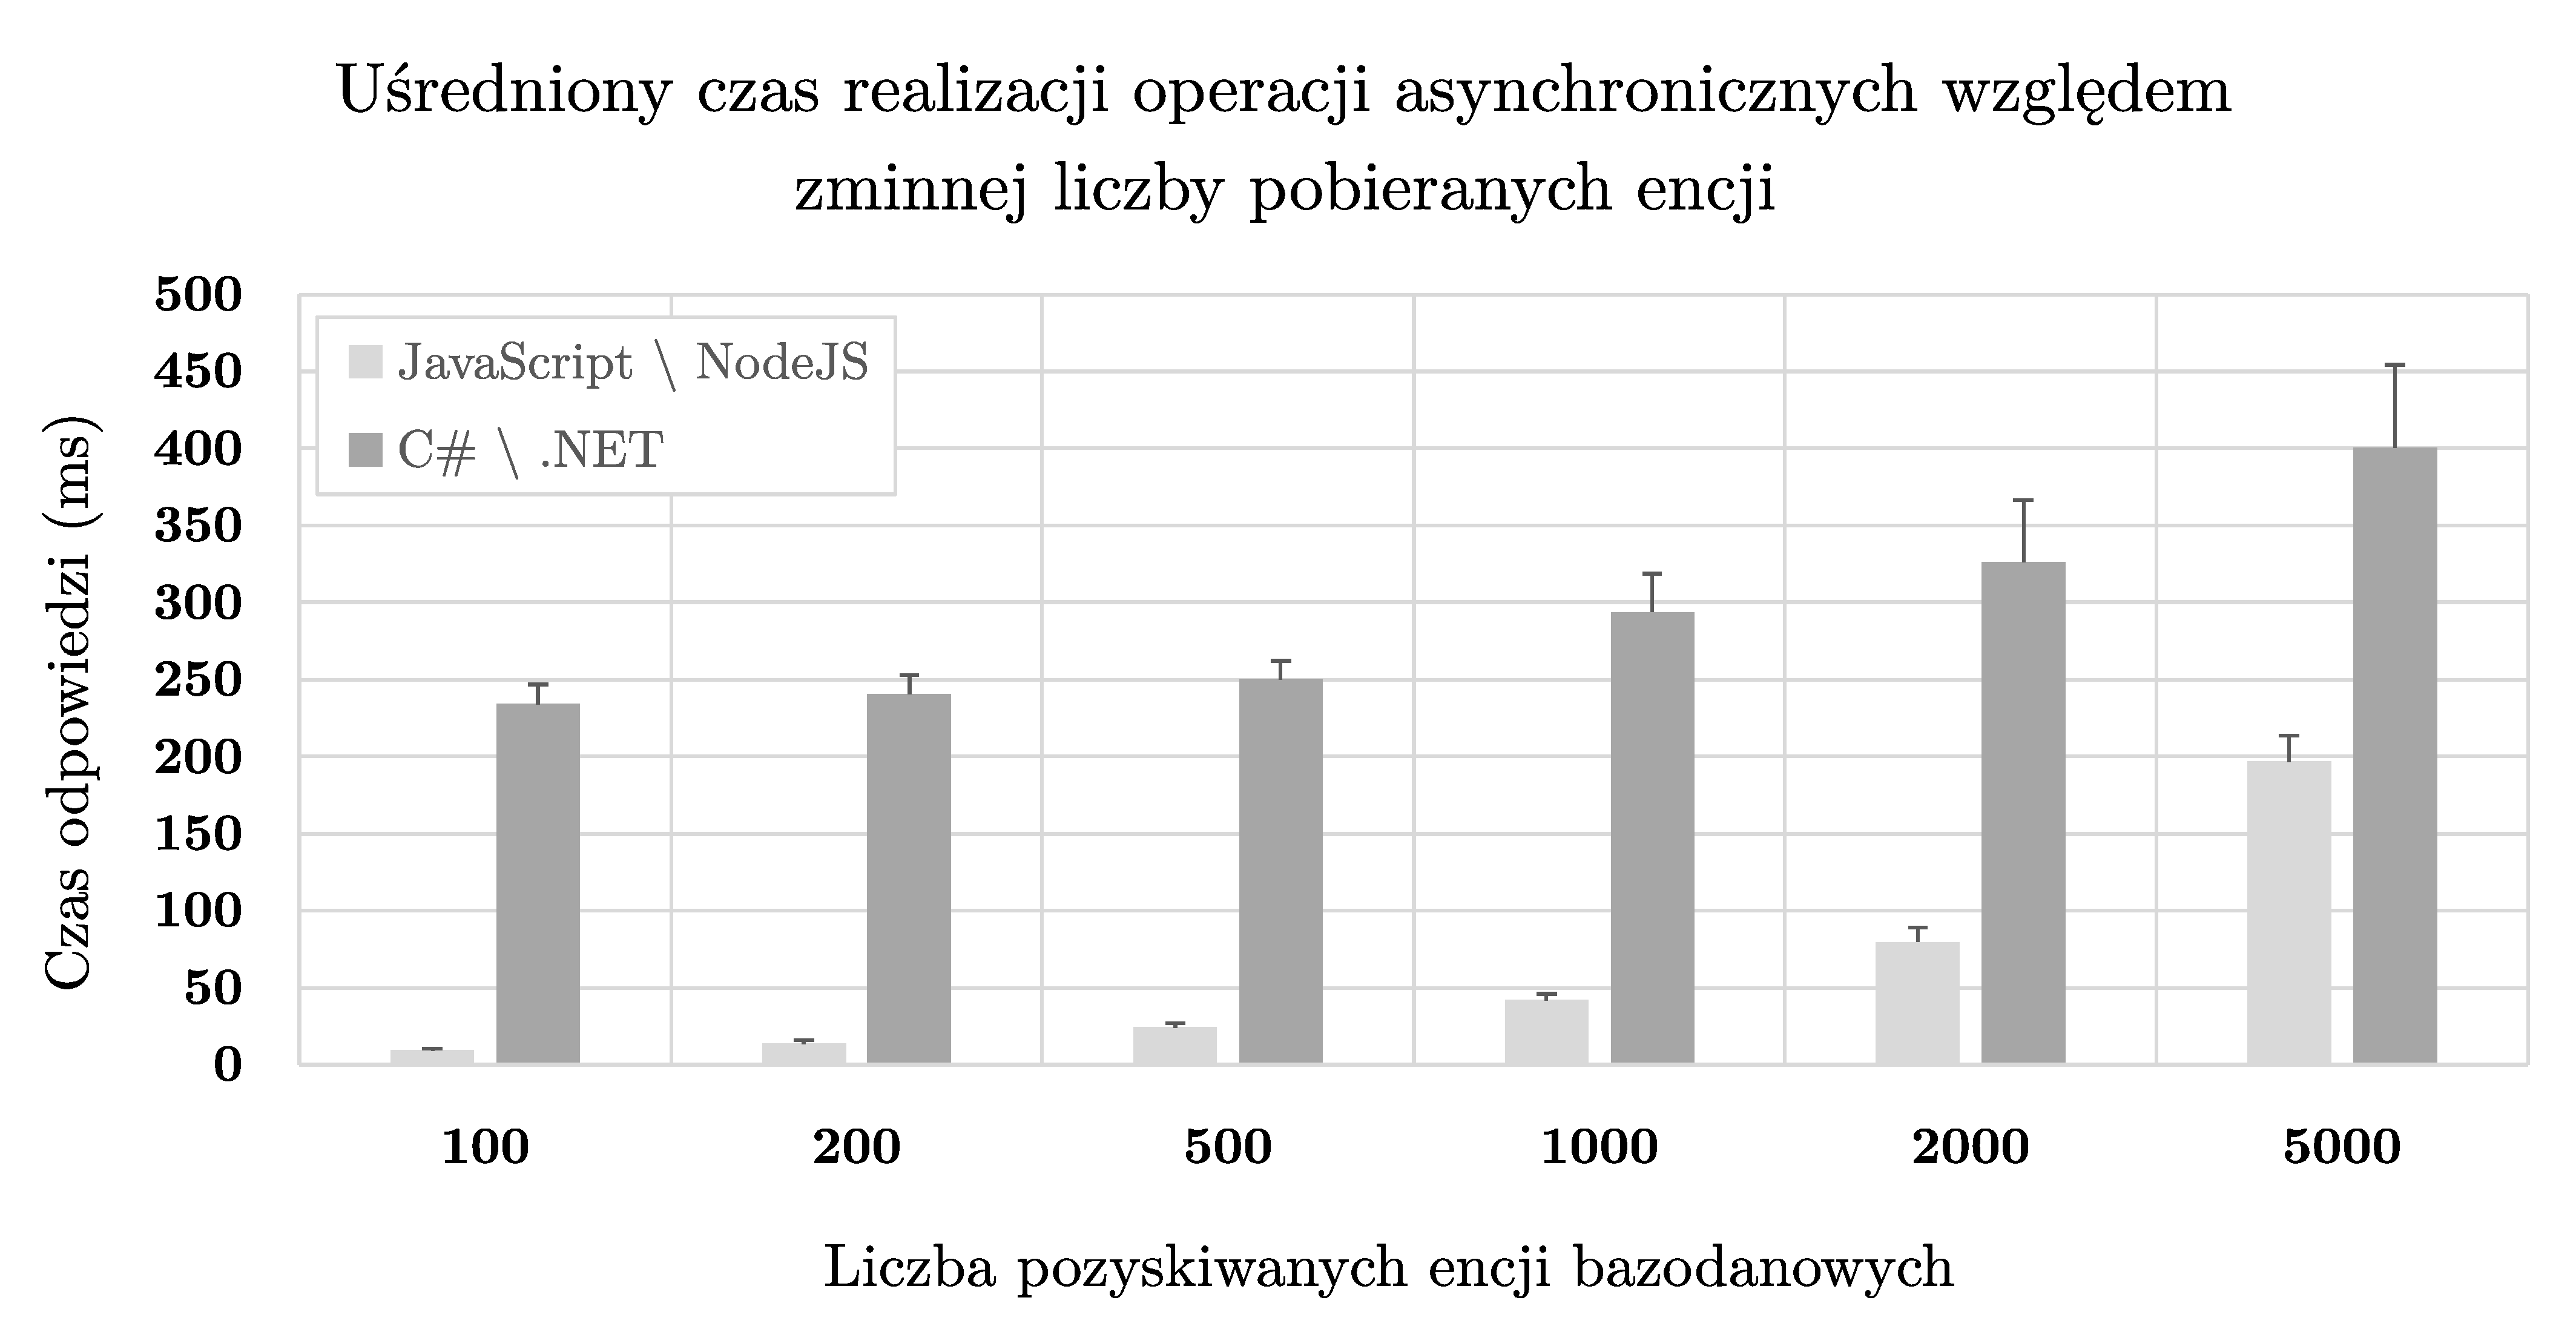
\includegraphics[width=\linewidth]{rys05/async-times.pdf}
  \caption{Uśredniony czas realizacji operacji asynchronicznych względem zmiennej liczby pobieranych encji}
  \label{fig:async-times}
\end{figure}

Zauważyć należy znaczącą wyższość rozwiązania opartego o technologie JavaScript / NodeJS, względem oprogramowania utworzonego z wykorzystaniem C\# .NET. Dla najmniejszej liczby pozyskiwanych encji, różnica średnich czasów odpowiedzi jest ponad 25 krotna. Wraz ze zwiększaniem liczebności pozyskiwanych obiektów modelu danych średni czas odpowiedzi dla NodeJS rośnie co prawda w szybszym tempie, niż ma to miejsce w kontekście rozwiązania uruchamianego na platformie .NET, jednakże nawet dla największej spośród liczb encji, dysproporcja wyników jest ponad dwukrotna. Warto zwrócić również uwagę na dyspersję poszczególnych rozwiązań względem przedstawionych średnich. Zaobserwować można zdecydowanie mniejsze odchylenia standardowe w odniesieniu do rozwiązania języka JavaScript, które zgodnie ze spodziewaną tendencją zwiększają się wraz z liczbą obiektów modelu danych. Dla dużych liczebności encji bazodanowych, rozwiązanie implementowane w języku C\# w niewielkiej liczbie przypadków uzyskuje wyniki bliskie średniej.

Tak znacząca dyferencja w kontekście obu interfejsów programowania aplikacji, wynikać może z implementacji natywnych rozwiązań klienta protokołu hipertekstowego. W środowisku NodeJS, klient ten posiada niewiele opcji konfiguracyjnych, a jakiekolwiek bardziej zaawansowane żądania, realizowane są z wykorzystaniem zewnętrznych bibliotek. Ponadto, klient ten, jest częścią rdzennego modułu środowiska NodeJS, obsługującego zoptymalizowaną komunikację hipertekstową. Rozwiązanie służące do komunikacji HTTP dla języka C\# jest mechanizmem dostarczanym przez biblioteki standardowe języka programowania, a nie samego środowiska uruchomieniowego. Oznacza to, że rozwiązanie dla tej właśnie technologii musi posiadać bardziej generyczną charakterystykę, aby móc być zastosowanym w dowolnym z przypadków użycia języka.
\section{Wpływ implementacji wzorca projektowego CQRS na wydajność obsługi żądania}
\label{sec:cqrs-and-database-improvements}
Celem niniejszego badania była obserwacja wpływu wdrożenia wzorca projektowego podziału odpowiedzialności, a także usprawnień wydajnościowych względem odseparowanych modeli encji, na wydajność obsługi żądań dla ocenianych interfejsów programowania aplikacji. Wdrożenie wzorca projektowego miało na celu odseparowanie operacji dotyczących odczytu danych, od tych, dokonujących ich modyfikacji. Separacja ta, występowała zarówno na poziomie logicznym (tj. modelu danych), jak i fizycznym (tj. systemu bazodanowego). Dzięki temu, możliwe było wprowadzenie optymalizacji wydajnościowych względem modelu odczytu. Aby zachować spójność informacji pomiędzy bazami danych, wprowadzono ponadto mechanizm replikacji transakcyjnej, działający w warstwie systemu bazodanowego. Po wysłaniu wiadomości modyfikującej dane, określony rekord jest zmieniany w bazie zapisu, a następnie wysyłany jest komunikat synchronizacji zmian w kierunku bazy odczytu. Szczegóły implementacyjne dotyczące omawianego badania przedstawiono w sekcji \ref{sec:implementacja-cqrs-i-replikacji}.

Zastosowany protokół badawczy posiada analogiczną strukturę do tego, który został zaprezentowany w badaniu wpływu systemów bazodanowych. Oznacza to, że w przedziale dwudziestu minut, stopniowo zwiększano liczbę współbieżnie pracujących wątków oprogramowania testowego, osiągając szczytową wartość równą 5000. W tym przypadku jednak, poddano analizie tylko pojedynczy system bazodanowy, który wspiera obsługę mechanizmu replikacji transakcyjnej - tj. Microsoft SQL Server. Kluczowym aspektem badania jest próba obserwacji czy, a także w jaki sposób wprowadzony model architektoniczny oraz usprawnienia wydajnościowe wpłyną na zmniejszenie się średniego czasu odpowiedzi, a także procentu błędnych odpowiedzi w stosunku do generowanych wiadomości. W badaniu zastosowano topologię fizyczną nr 4 przedstawioną w sekcji \ref{sec:lokalne-srodowisko-badawcze-ver-4}, a także plan testowy nr 1 wyszczególniony w punkcie \ref{plan-testowy-1}. Ogół przeprowadzonych operacji jest zgodny z wyspecyfikowanym scenariuszem badawczym nr 4 opisanym w tabeli \ref{tab:research-scenario-4}.

Na wykresach \ref{fig:3tier-vs-cqrs} a) do \ref{fig:3tier-vs-cqrs} d) przedstawiono kolejno porównanie procedur odczytu oraz zapisu, zarówno przed jak i po zastosowaniu omówionych modyfikacji.

\begin{figure}[htb]
  \centering
    \begin{tabular}{@{}ll@{}}
    a) & b) \\
    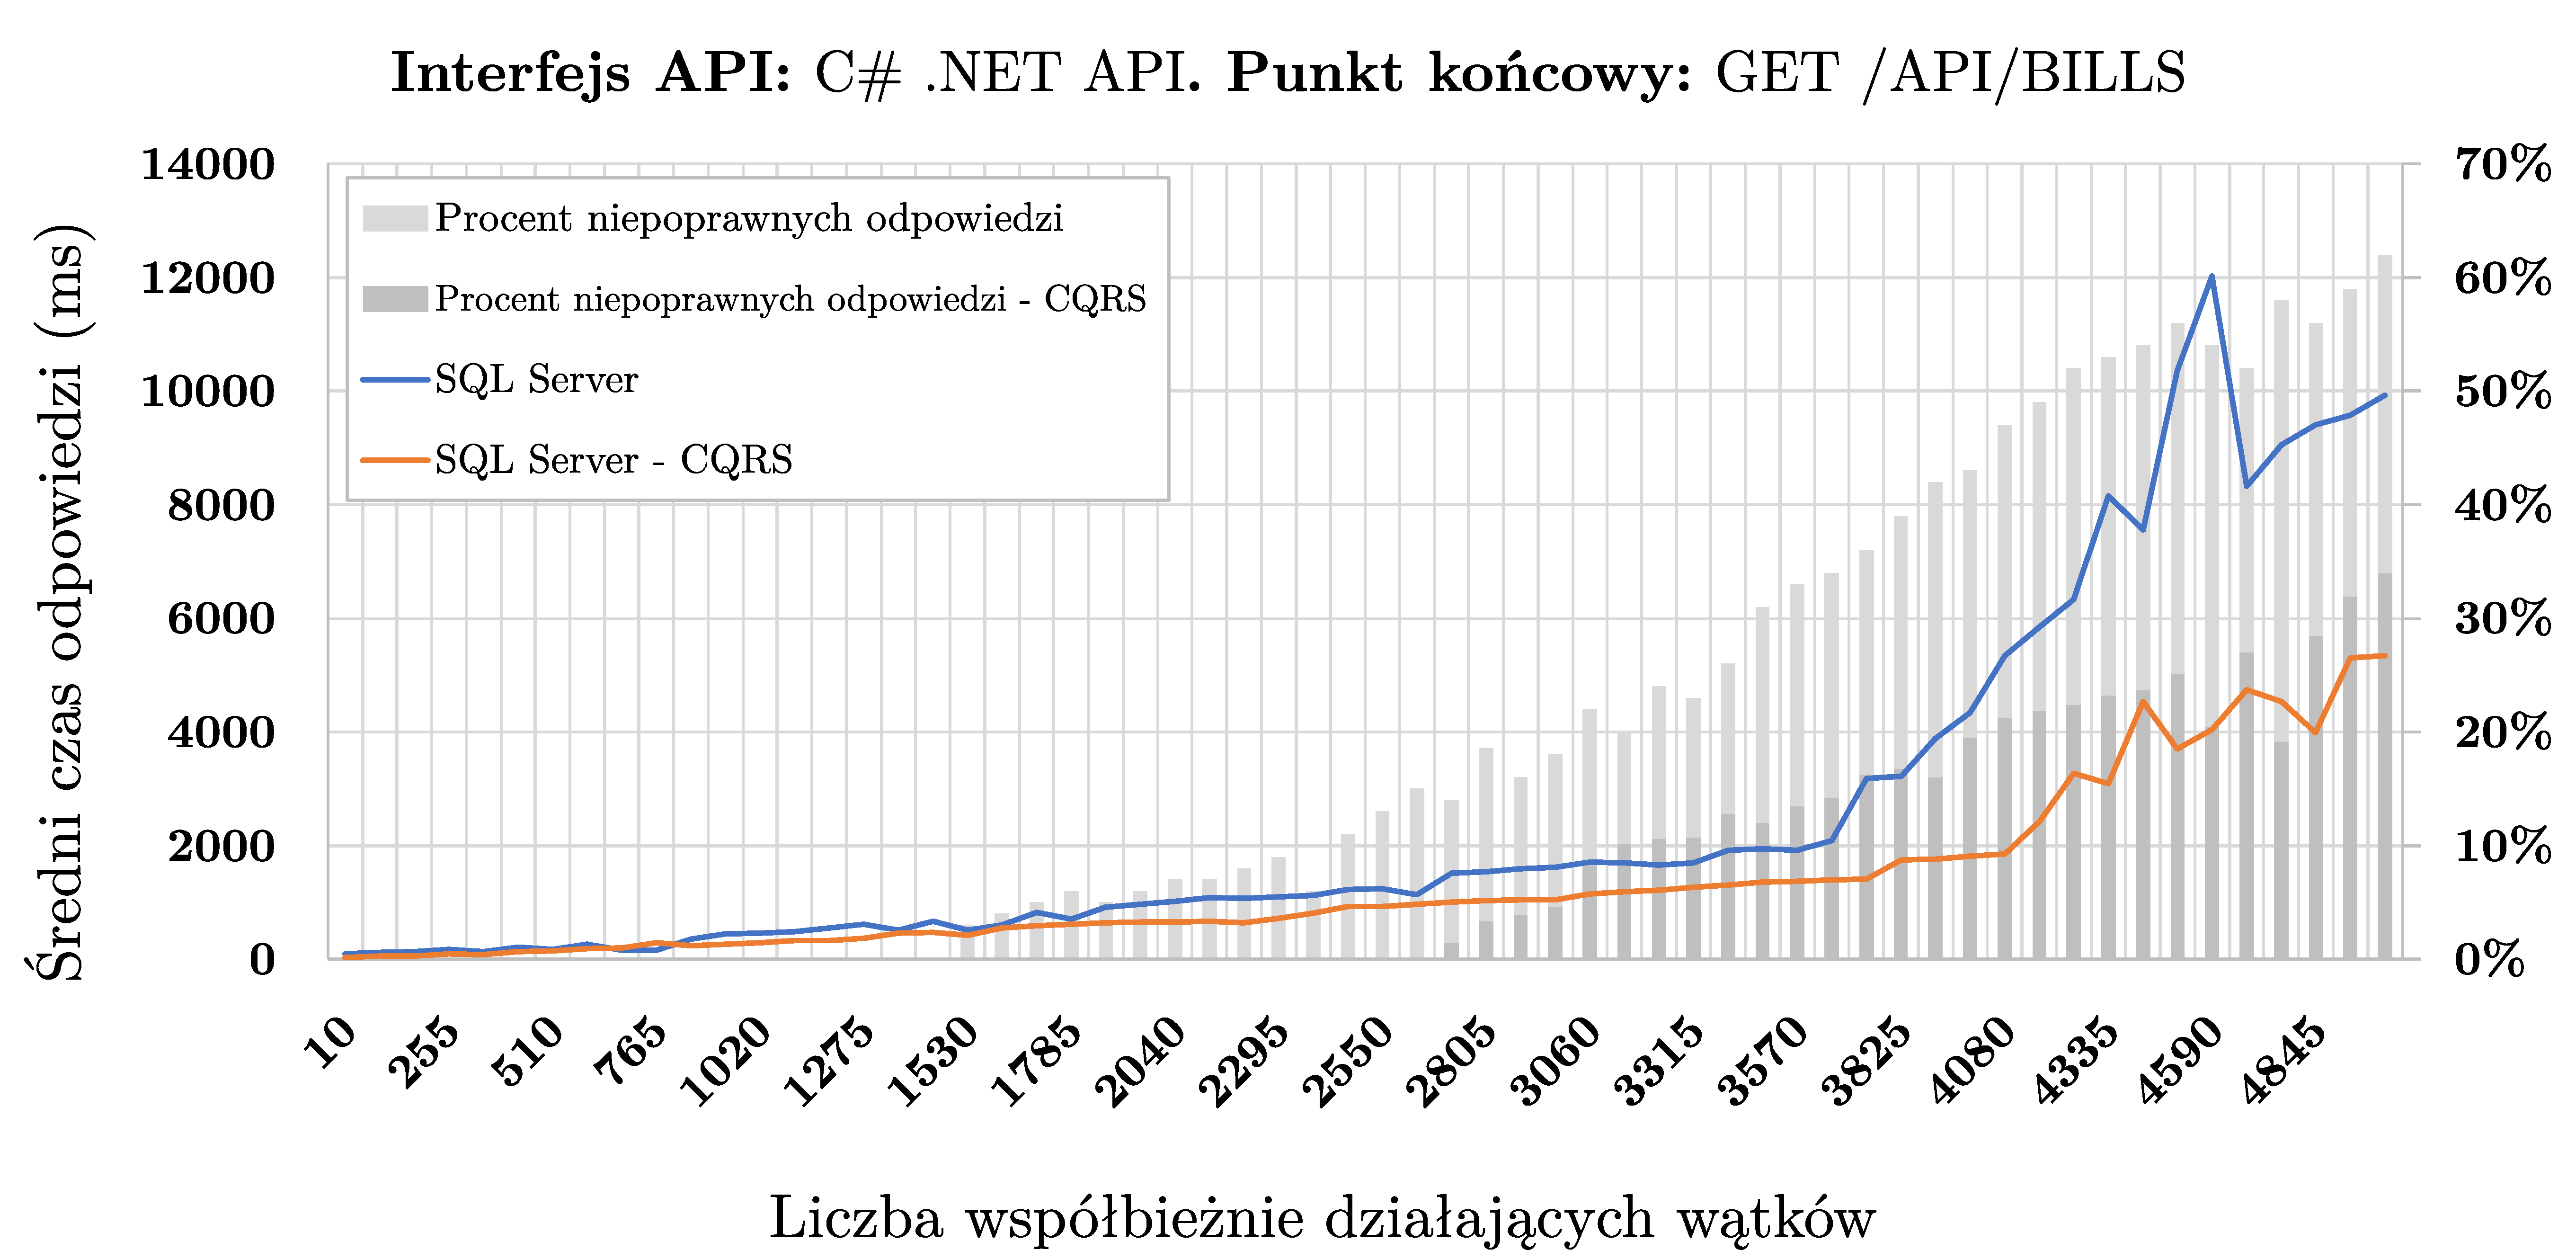
\includegraphics[width=0.49\textwidth]{rys05/dotnet-vs-cqrs.pdf} & 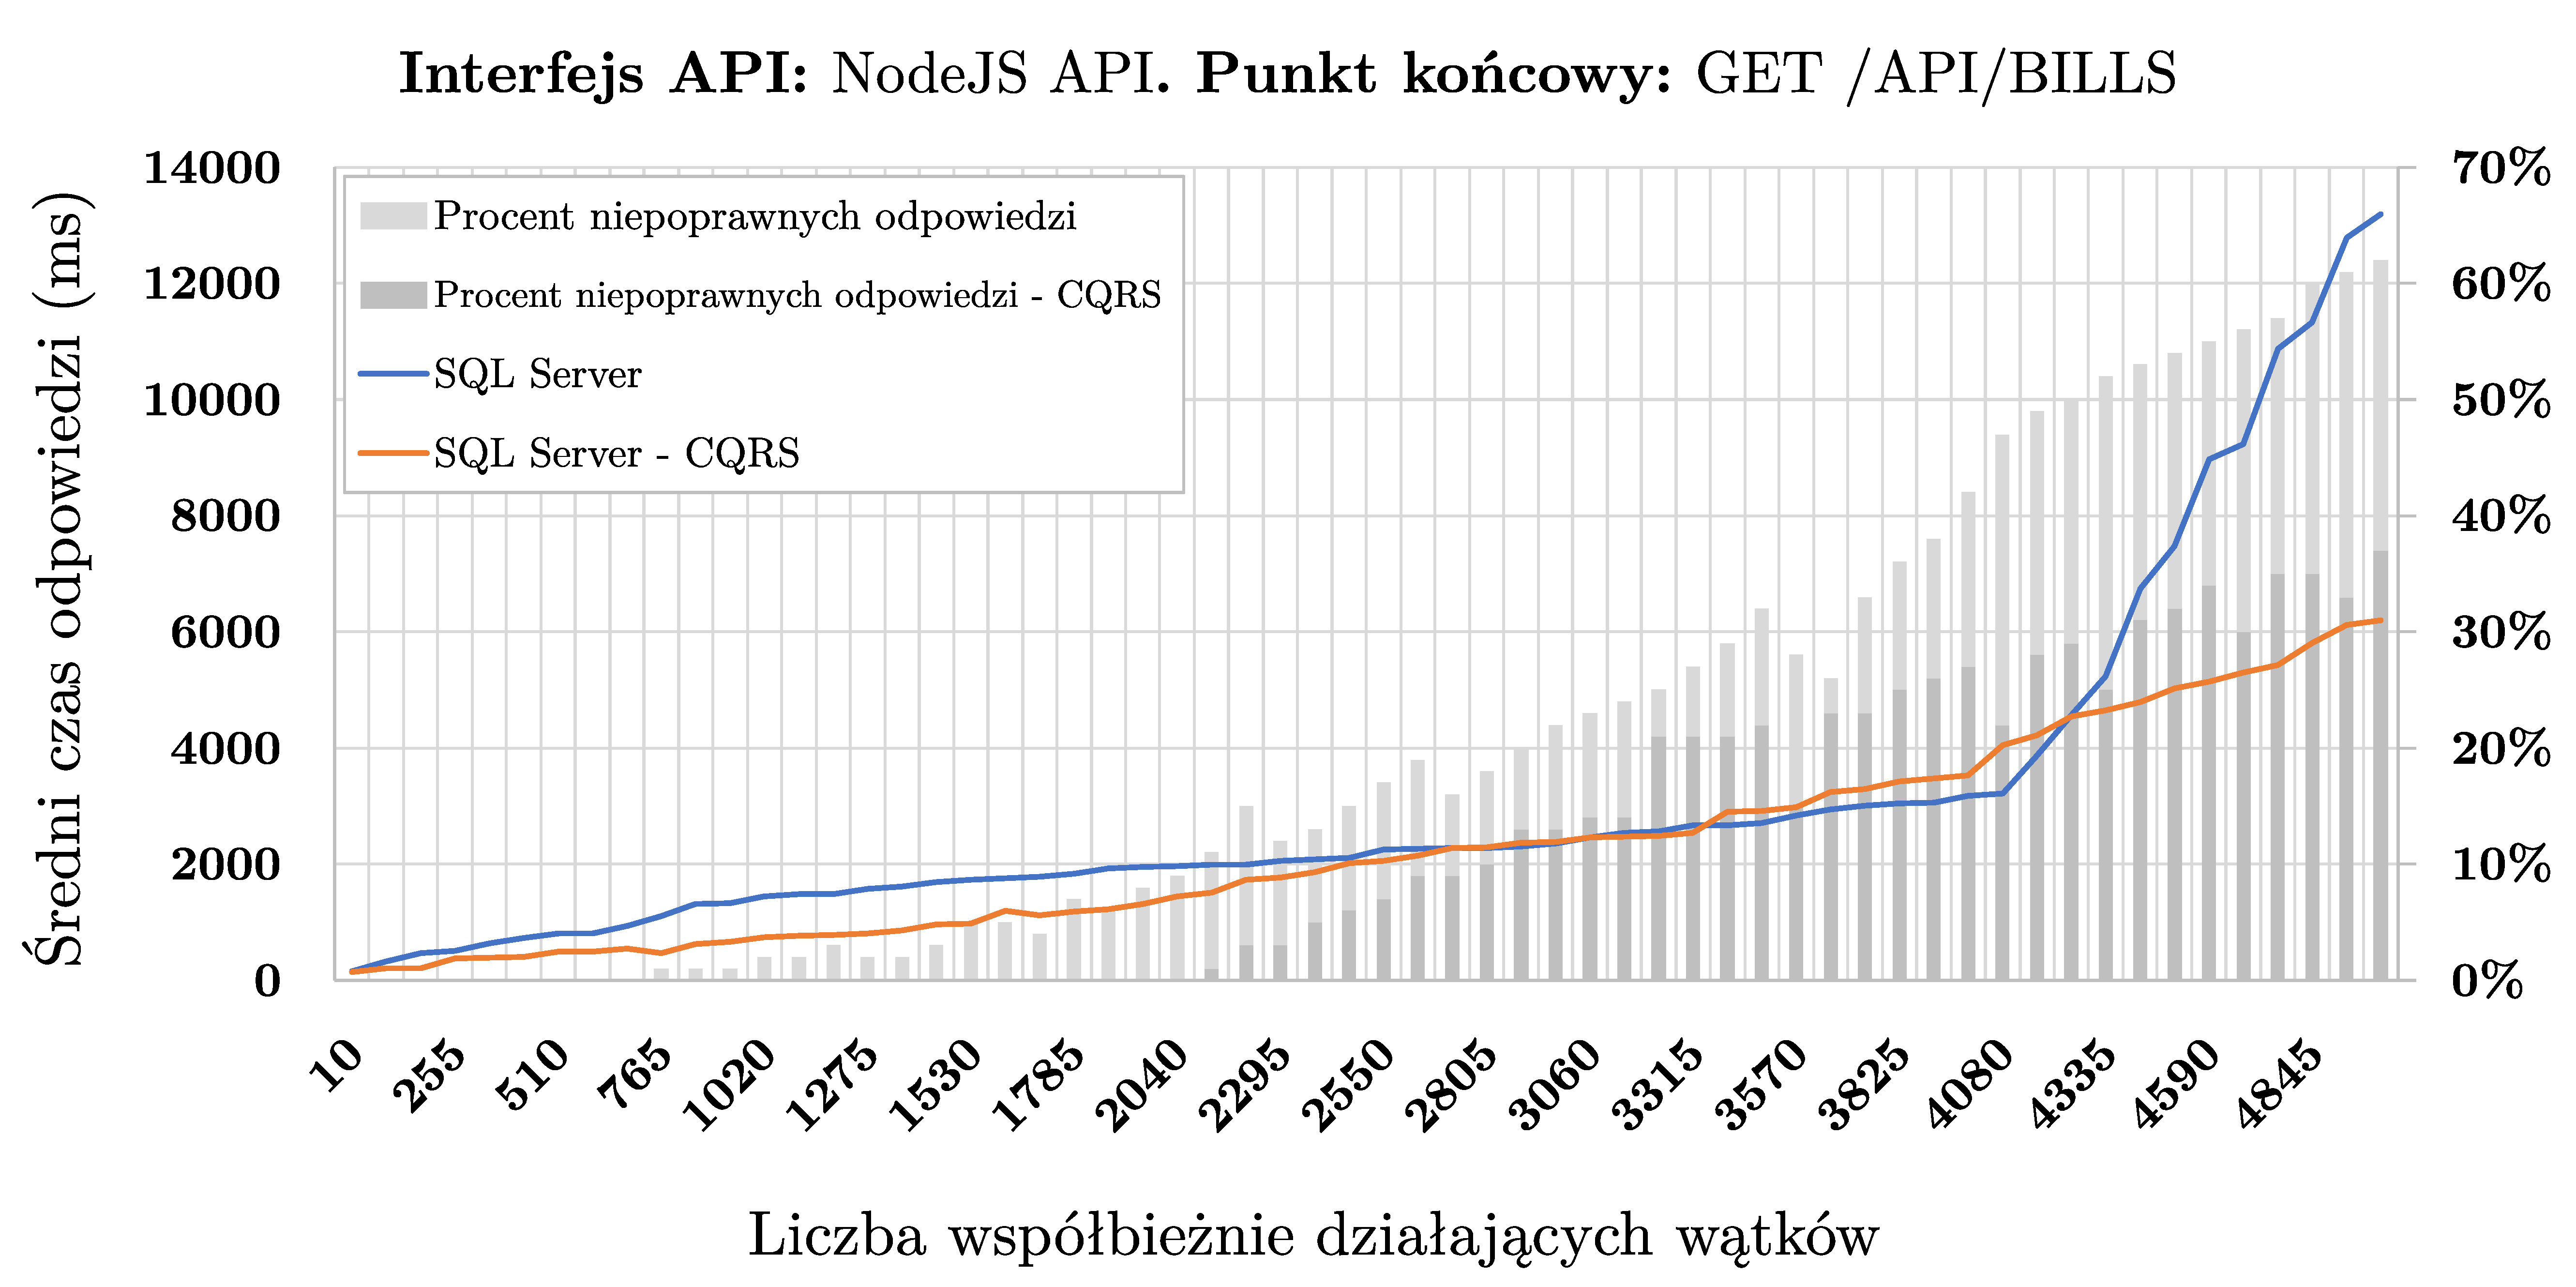
\includegraphics[width=0.49\textwidth]{rys05/nodejs-vs-cqrs.pdf} \\
    c) & d) \\
    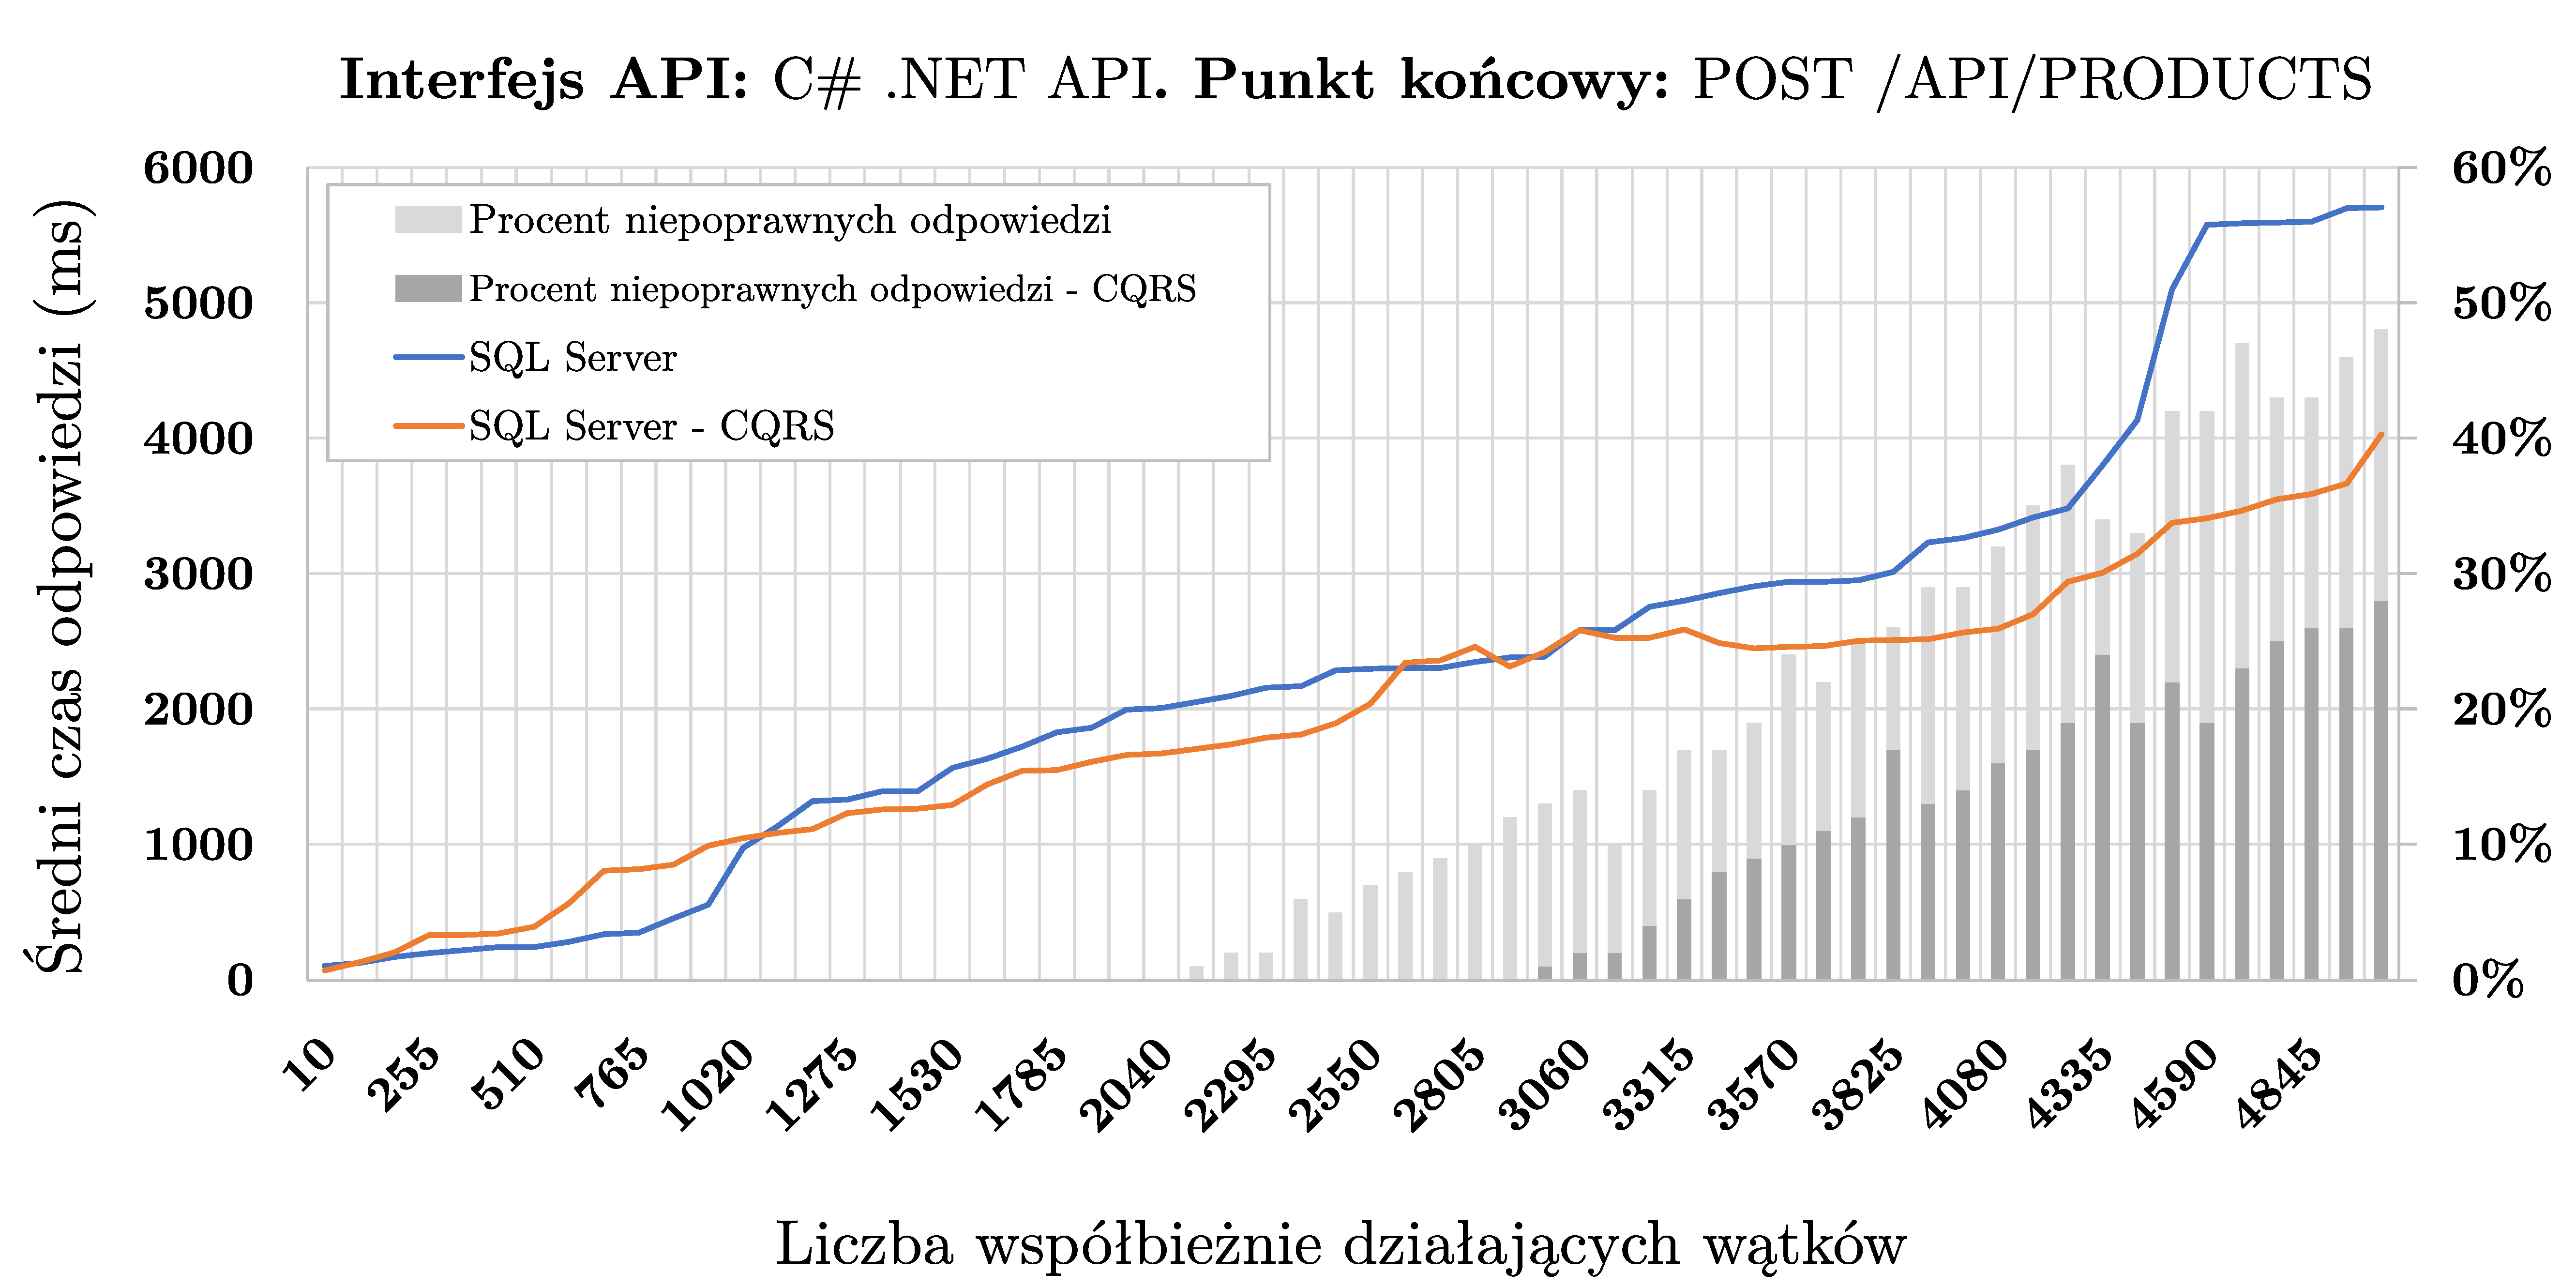
\includegraphics[width=0.49\textwidth]{rys05/dotnet-vs-cqrs-write.pdf} & 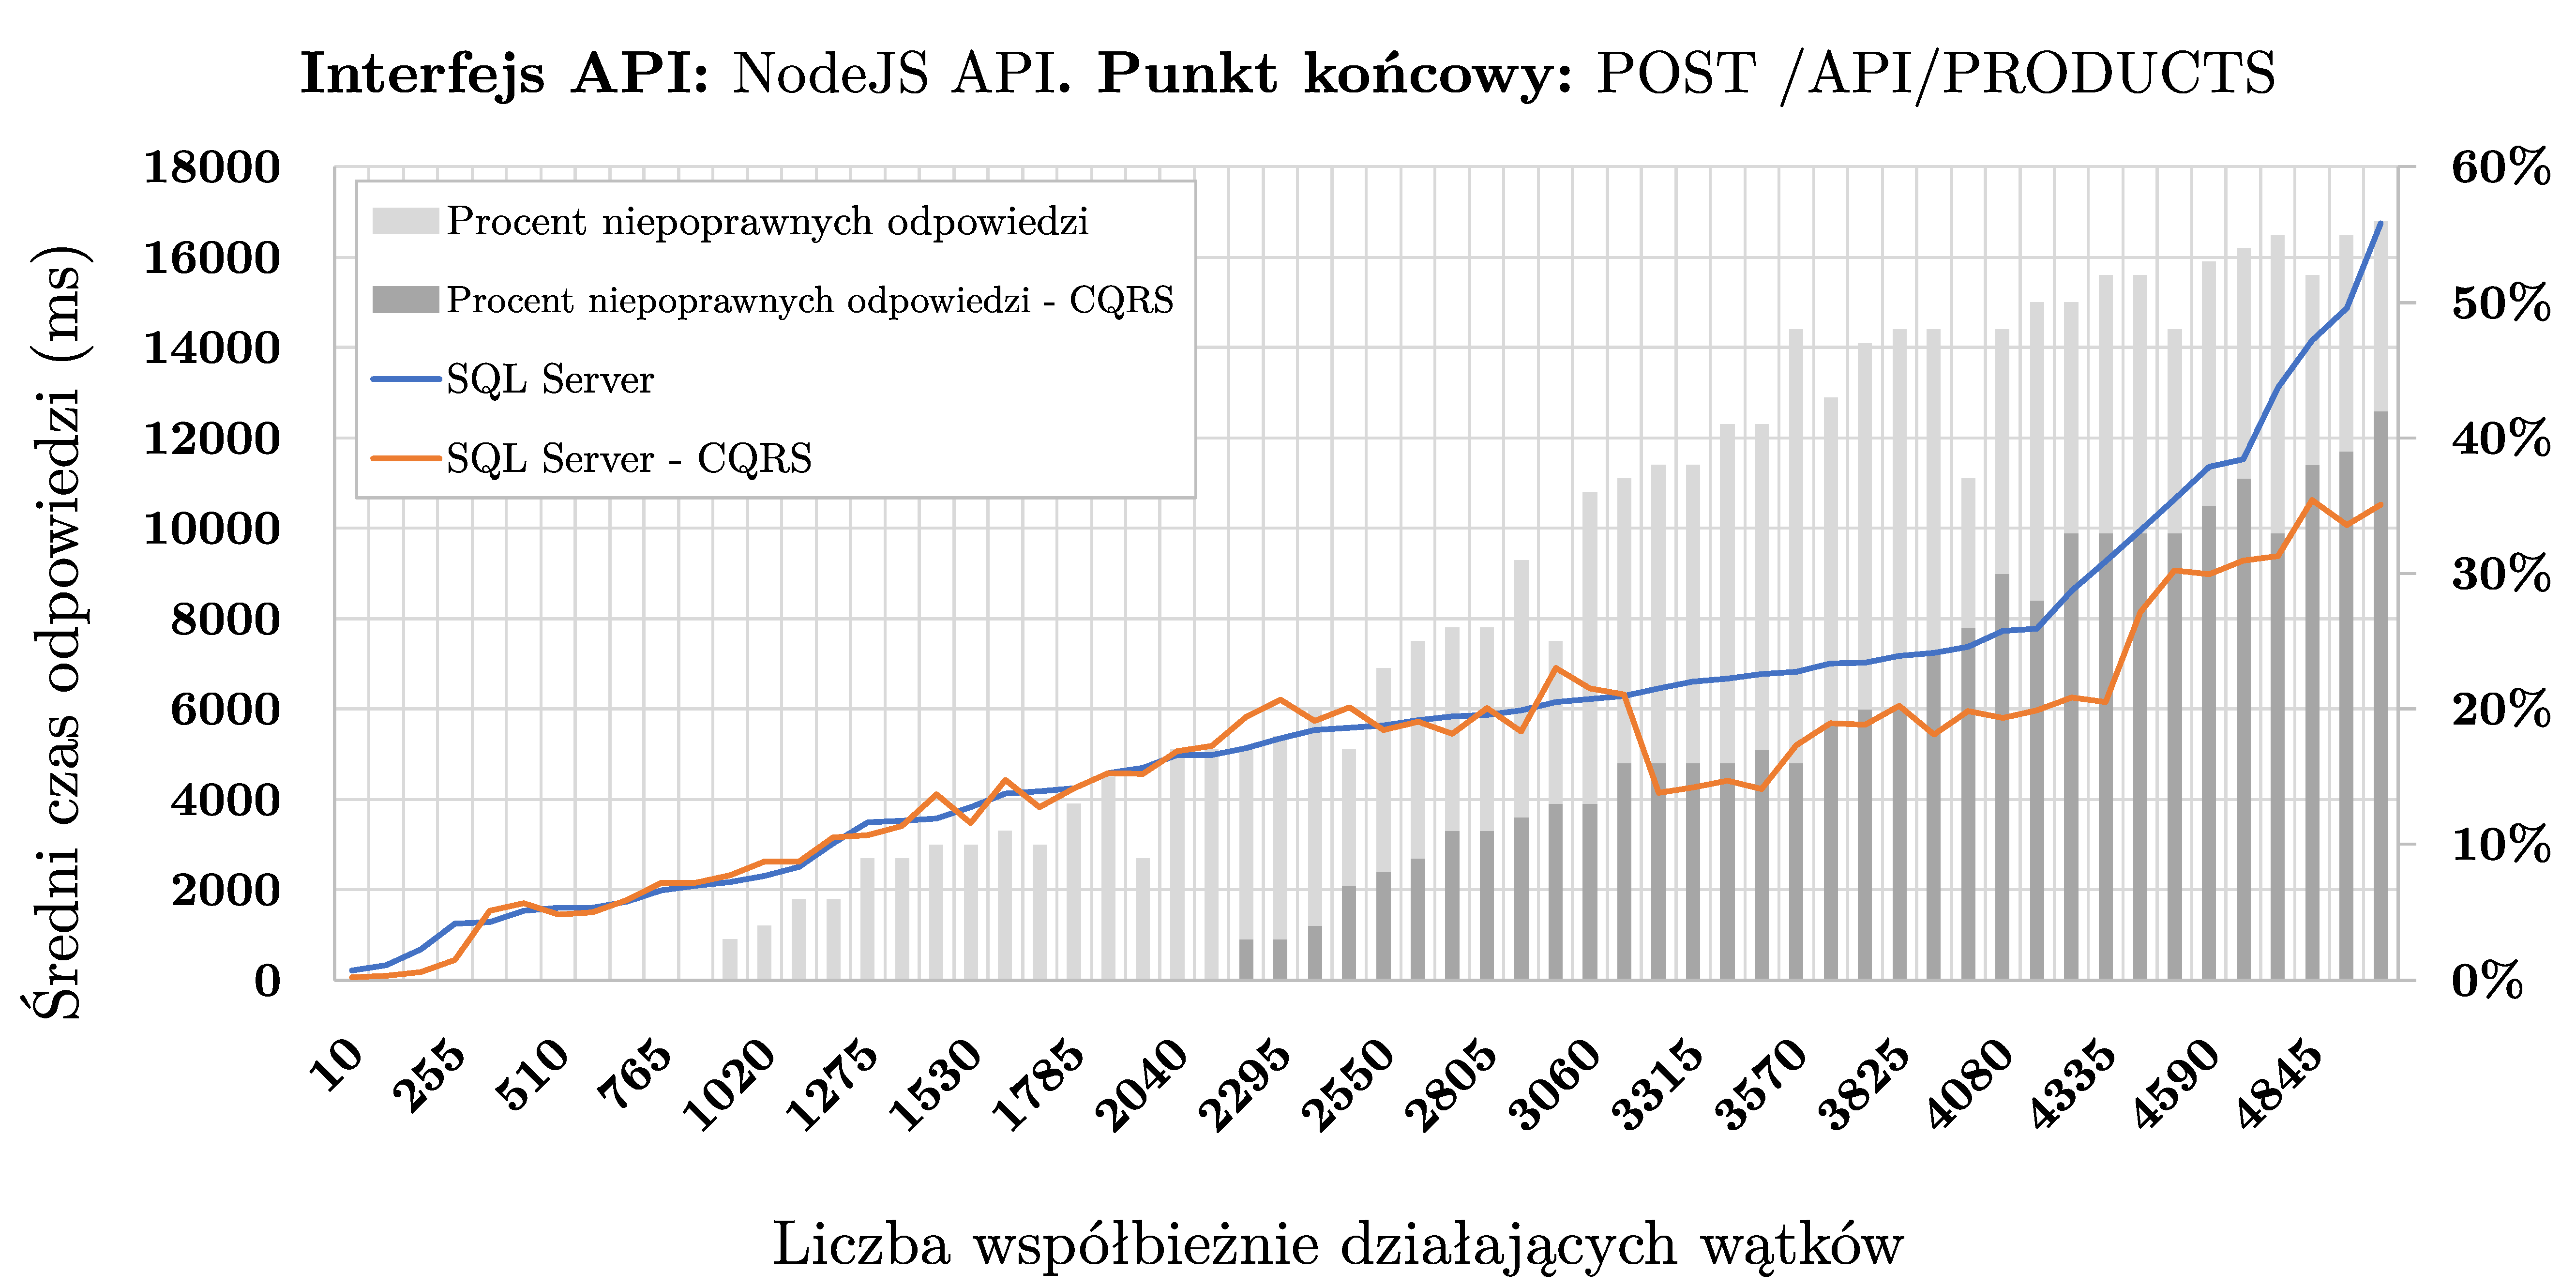
\includegraphics[width=0.49\textwidth]{rys05/nodejs-vs-cqrs-write.pdf}
    % jezeli obraki sa rownej wysokosci, mozna je wyrownac do gory stosujac vtop jak nizej
    % \vtop{\vskip-2ex\hbox{{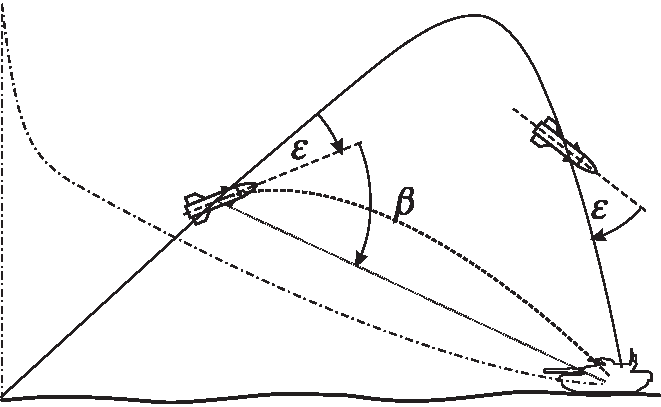
\includegraphics[width=0.475\textwidth]{rys05/beta1}}}} &
    % \vtop{\vskip-2ex\hbox{{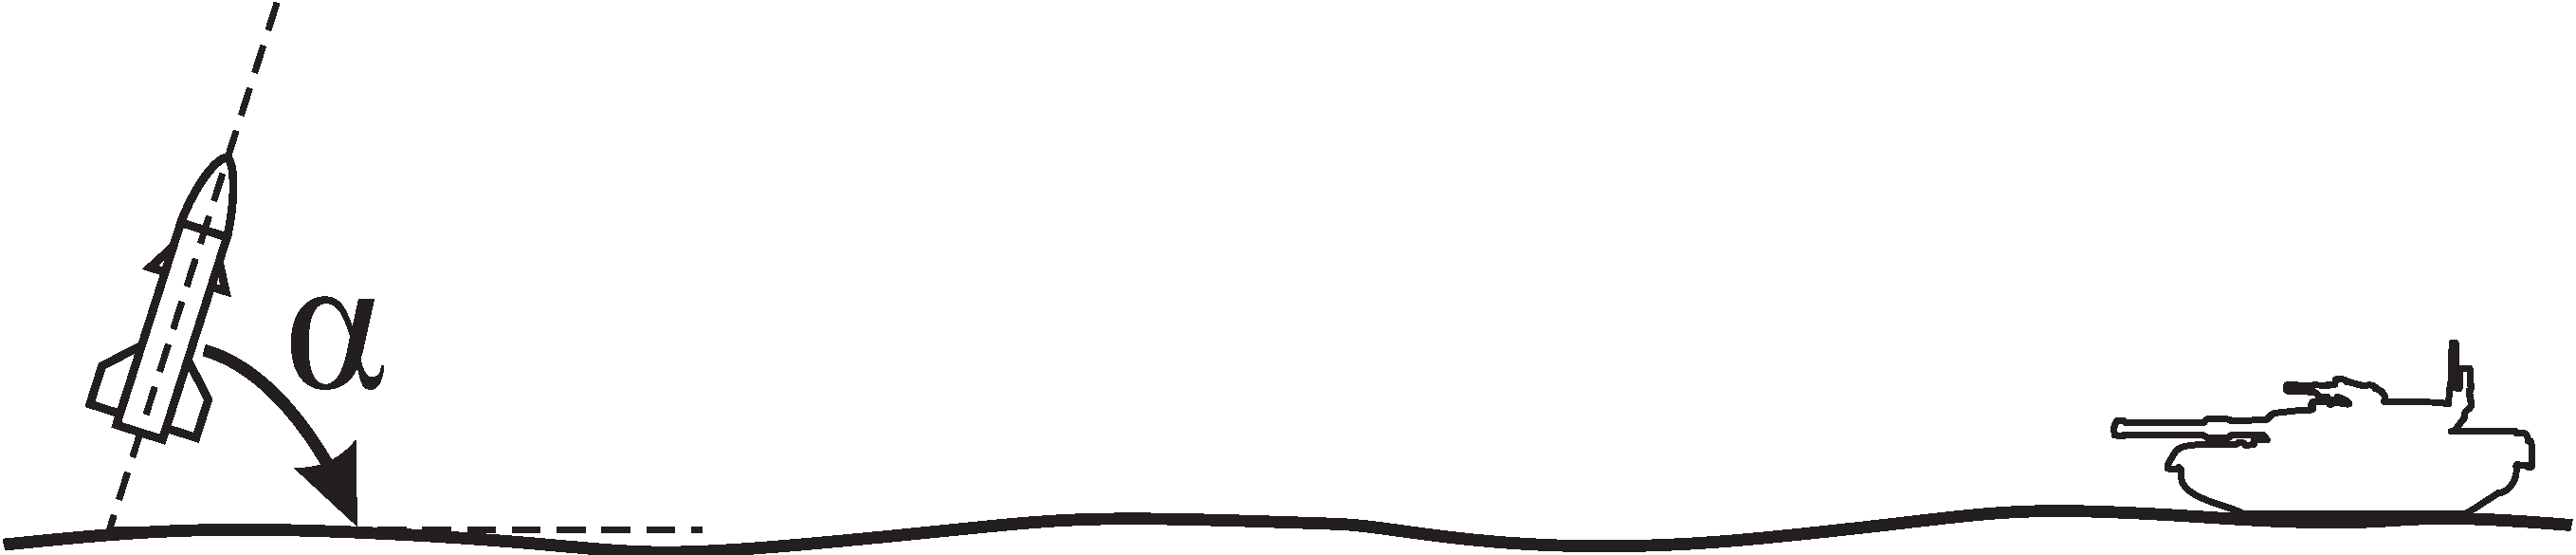
\includegraphics[width=0.475\textwidth]{rys05/alfa1}}}}  \caption{Wyznaczanie trajektorii lotu rakiety: 
    \end{tabular}
  \caption{Wydajność działania interfejsów API dla operacji odczytu oraz zapisu, przed i po zastosowaniu wzorca podziału odpowiedzialności}
  \label{fig:3tier-vs-cqrs}
\end{figure}

Dla każdego z przypadków zauważyć należy zarówno obniżenie się poziomu średniego czasu odpowiedzi, jak i procentowego błędu żądań niepoprawnych. Zachowanie takie, jest zrozumiałe ze względu na silną korelację obu metryk. Dostrzec należy relatywnie większą zmianę średniego czasu odpowiedzi w kontekście odczytu danych, niż ma to miejsce dla procedury ich zapisu. Wynika to z faktu, że dla zadania odczytu, dokonano usprawnień nie tylko związanych z komunikacją z bazą danych (m.in. zdefiniowanie puli połączeń), ale również dotyczących formułowania zapytań, czy też wewnętrznej struktury poszczególnych pól danych. Wpływ pierwszego z wymienionych w poprzednim zdaniu aspektów widoczny jest szczególnie w odniesieniu do zmiany procenta niepoprawnych żądań. Tyczy się to zarówno procedury odczytu, jak i zapisu. Co więcej metryka ta, wpływa na średni czas odpowiedzi. Czym więcej kanałów komunikacji z serwerem bazodanowym posiada interfejs API, tym więcej żądań będzie mógł on obsłużyć bez konieczności czekania na zwolnienie połączenia.

Dla procedury odczytu danych, po wprowadzeniu opisywanych w niniejszym badaniu usprawnień, pierwszy błąd związany z niepoprawną obsługą zapytania, pojawił się przy natężeniu o \textbf{1273} wątki wyższym dla api napisanego w technologii C\# .NET, oraz o \textbf{1527} wątków wyższym w przypadku NodeJS API. W kontekście metryki czasu wykonywania zapytania klienta, w momencie szczytowym zauważyć można różnicę \textbf{4577 ms} dla rozwiązania C\# oraz \textbf{6987 ms} dla systemu opartego o NodeJS.

Odnosząc się do procedury zapisu danych, przedział liczby wątków oprogramowania testowego, w ramach którego nie wystąpiły błędne żądania, rozszerzył się o \textbf{1190} procesów w przypadku interfejsu napisanego w języku JavaScript, a także o \textbf{765} procesów w przypadku api implementowanego w C\#. Doprowadziło to do spadku średniego czasu odpowiedzi w momencie szczytowym o \textbf{6225 ms} dla pierwszej z wymienionych technologii, a także o \textbf{1677 ms} dla drugiej z nich.

Analizując powyższe rezultaty, należy także spojrzeć na nie przez pryzmat ilości zmian, jakie zostały wprowadzone dla poszczególnych technologii. Mówiąc o interfejsie programowania aplikacji języka JavaScript, modyfikacje sprowadzały się do usprawnień na poziomie bazy danych, a także w kontekście momentu uruchamiania instancji mapera obiektowo-relacyjnego. Pomimo stosunkowo niewielkiej liczby zaimplementowanych adaptacji, wydajność rozwiązania wzrosła w sposób znaczący. Lekko odmienną tendencję zauważyć można dla usługi sieciowej napisanej w języku C\#. W tym przypadku wprowadzono nie tylko analogiczne względem konkurenta poprawki, ale także dodatkowo skorzystano z mechanizmów poprawy wydajności, specyficznych względem tylko tej technologii. Co prawda implementacja określonych modyfikacji wpłynęła pozytywnie na efektywność działania interfejsu, to zmiana ta, nie jest tak znacząca, jak dla rozwiązania opartego o technologię JavaScript / NodeJS. 
\section{Porównanie efektywności obsługi zapytań dla odmiennych mechanizmów pamięci podręcznej}
W przedstawionym badaniu dokonano porównania wydajności obsługi żądań klienckich, dotyczących pozyskiwania obiektów danych, w odniesieniu do wykorzystania zaimplementowanych mechanizmów pamięci podręcznej. Wydajność w ramach przeprowadzonej ewaluacji rozumiana była poprzez czas odpowiedzi na żądanie. Warto zaznaczyć, że nie uwzględniono parametru dotyczącego liczby niepoprawnych zapytań ponieważ dla żadnej z próbek, nie uzyskano nieprawidłowej odpowiedzi.

Zdecydowano się na wdrożenie dwóch mechanizmów obsługi pamięci podręcznej. Działanie pierwszego z nich, nazywanego mechanizmem statycznym, polega na zapamiętywaniu odpowiedzi w kontekście żądania o określonych właściwościach (tj. identyfikator zasobu, parametry zapytania), a także przetrzymywaniu jej w buforze przez stały, określony czas. Jeżeli zapytanie charakteryzujące się znaną uprzednio strukturą, zostanie odebrane w tym właśnie czasie, odpowiedź nie zostanie pobrana z bazy danych, a dostarczona bezpośrednio z omawianego bufora. Drugi mechanizm jest autorskim pomysłem twórcy niniejszej pracy i uwzględnia zmienność czasu przechowywania wpisu w odniesieniu do częstości wywoływań, a także unieważnień danych przechowywanych w pamięci cache. Mechanizm ten, wykorzystuje ponadto osobną strukturę danych, która jest aktualizowana przy wywołaniu dowolnego punktu końcowego, a gromadzone w niej dane, dostarczają informacji niezbędnych do wyliczania czasu zapamiętywania wpisu w cache. Niezależnie od omawianego mechanizmu, punkty końcowe odpowiedzialne za modyfikację danych, dla których wpisy przechowywane są w pamięci podręcznej, uruchamiają procedurę unieważnienia określonych obiektów encji. Szczegóły implementacyjne dotyczące obu mechanizmów pamięci podręcznej przytoczone zostały w sekcji \ref{sec:mechanizmy-cache}.

Odnosząc się do procedury badawczej, wykonane zostało 20 eksperymentów, w ramach których 30 współbieżnie pracujących wątków generowało żądania w kierunku dwóch punktów końcowych. Pierwszy z nich, dotyczył pobrania listy encji o stałym rozmiarze, natomiast drugi -- uzyskania pojedynczego obiektu danych. Dla każdej z ewaluacji, przeprowadzanej w kontekście określonego interfejsu programowania aplikacji, zdefiniowano pięć zdarzeń unieważnienia danych (tj. momentów wywołania punktu końcowego modyfikującego encje). Ponadto zaznaczyć należy, że czas trwania pojedynczego eksperymentu był stały i wynosił 20 minut. Co więcej, wprowadzona została celowa dysproporcja pomiędzy liczbą żądań pozyskujących listę obiektów, a liczbą zapytań, których rezultatem jest zwrócenie tylko jednego z nich. Stosunek ten, wynosił dwa do jednego. Taka struktura badań, wynika z charakterystyki dotyczącej sposobu wyliczania czasu przechowywania wpisu w pamięci podręcznej w odniesieniu do autorskiego mechanizmu. Promuje on, te spośród żądań, których częstotliwość wywołań jest większa.

Dla statycznego mechanizmu pamięci cache zastosowano czas życia wynoszący 60s, podczas gdy czasem referencyjnym mechanizmu autorskiego było 120s. Co więcej, wewnętrzna struktura wykorzystywana w rozwiązaniu autorskim, została wygenerowana na podstawie liczby żądań wysłanych w czasie realizacji eksperymentu ze stałym czasem przechowywania wpisu. Dzięki temu, punkt końcowy dotyczący pobierania listy elementów, był postrzegany jako element wywoływany z większą częstotliwością.

Badanie przeprowadzono zgodnie z koncepcją zarysowaną w scenariuszu badawczym nr 5, którego elementy wyspecyfikowano w tabeli \ref{tab:research-scenario-5}, a także wykorzystując konfigurację nr 2 lokalnej topologii fizycznej przedstawionej w sekcji \ref{sec:lokalne-srodowisko-badawcze-ver-2}.

W tabeli \ref{tab:mtc-5-table} zaprezentowano elementy charakterystyczne dla każdego z dwudziestu eksperymentów, a także rezultaty jakie w kontekście nich odnotowano.

\begin{table}[H] \small
\centering
\caption{Wydajność metod obsługi pamięci podręcznej względem technologii oraz momentu unieważnienia wpisu}
\label{tab:mtc-5-table}
\resizebox{\columnwidth}{!}{%
\begin{tabular}{|l|l|ccccc|l|l|}
\hline
\multirow{2}{*}{} &
  \multirow{2}{*}{Typ metody} &
  \multicolumn{5}{c|}{Moment unieważnienia} &
  \multirow{2}{*}{\begin{tabular}[c]{@{}l@{}}Liczba żądań\\ \textgreater 500 ms\end{tabular}} &
  \multirow{2}{*}{\begin{tabular}[c]{@{}l@{}}Zysk względem\\ rozwiązania alternatywnego\end{tabular}} \\ \cline{3-7}
  &
   &
  \multicolumn{1}{c|}{\#1} &
  \multicolumn{1}{c|}{\#2} &
  \multicolumn{1}{c|}{\#3} &
  \multicolumn{1}{c|}{\#4} &
  \#5 &
   &
   \\ \hline\hline\
\multirow{2}{*}{C\# / .NET} &
  statyczna &
  \multicolumn{1}{c|}{06:40} &
  \multicolumn{1}{c|}{10:00} &
  \multicolumn{1}{c|}{13:20} &
  \multicolumn{1}{c|}{15:00} &
  19:40 &
  10 &
  - \\ \cline{2-9} 
 &
  \textbf{autorska} &
  \multicolumn{1}{c|}{06:40} &
  \multicolumn{1}{c|}{10:00} &
  \multicolumn{1}{c|}{13:20} &
  \multicolumn{1}{c|}{15:00} &
  19:40 &
  9 &
  13,77 ms \\ \hline
\multirow{2}{*}{C\# / .NET} &
  statyczna &
  \multicolumn{1}{c|}{00:32} &
  \multicolumn{1}{c|}{03:45} &
  \multicolumn{1}{c|}{06:52} &
  \multicolumn{1}{c|}{07:49} &
  16:40 &
  8 &
  20,16 ms \\ \cline{2-9} 
 &
  autorska &
  \multicolumn{1}{c|}{00:32} &
  \multicolumn{1}{c|}{03:45} &
  \multicolumn{1}{c|}{06:52} &
  \multicolumn{1}{c|}{07:49} &
  16:40 &
  12 &
  - \\ \hline
\multirow{2}{*}{C\# / .NET} &
  statyczna &
  \multicolumn{1}{c|}{02:44} &
  \multicolumn{1}{c|}{06:30} &
  \multicolumn{1}{c|}{14:27} &
  \multicolumn{1}{c|}{16:55} &
  19:42 &
  14 &
  - \\ \cline{2-9} 
 &
  \textbf{autorska} &
  \multicolumn{1}{c|}{02:44} &
  \multicolumn{1}{c|}{06:30} &
  \multicolumn{1}{c|}{14:27} &
  \multicolumn{1}{c|}{16:55} &
  19:42 &
  10 &
  12,54 ms \\ \hline
\multirow{2}{*}{C\# / .NET} &
  statyczna &
  \multicolumn{1}{c|}{01:15} &
  \multicolumn{1}{c|}{05:29} &
  \multicolumn{1}{c|}{08:31} &
  \multicolumn{1}{c|}{14:48} &
  17:45 &
  15 &
  - \\ \cline{2-9} 
 &
  \textbf{autorska} &
  \multicolumn{1}{c|}{01:15} &
  \multicolumn{1}{c|}{05:29} &
  \multicolumn{1}{c|}{08:31} &
  \multicolumn{1}{c|}{14:48} &
  17:45 &
  13 &
  19,29 ms \\ \hline
\multirow{2}{*}{C\# / .NET} &
  statyczna &
  \multicolumn{1}{c|}{02:01} &
  \multicolumn{1}{c|}{07:32} &
  \multicolumn{1}{c|}{12:00} &
  \multicolumn{1}{c|}{13:27} &
  15:56 &
  16 &
  24,85 ms \\ \cline{2-9} 
 &
  autorska &
  \multicolumn{1}{c|}{02:01} &
  \multicolumn{1}{c|}{07:32} &
  \multicolumn{1}{c|}{12:00} &
  \multicolumn{1}{c|}{13:27} &
  15:56 &
  20 &
  - \\ \hline
\multirow{2}{*}{JS / NodeJS} &
  statyczna &
  \multicolumn{1}{c|}{06:40} &
  \multicolumn{1}{c|}{10:00} &
  \multicolumn{1}{c|}{13:20} &
  \multicolumn{1}{c|}{15:00} &
  19:40 &
  17 &
  - \\ \cline{2-9} 
 &
  \textbf{autorska} &
  \multicolumn{1}{c|}{06:40} &
  \multicolumn{1}{c|}{10:00} &
  \multicolumn{1}{c|}{13:20} &
  \multicolumn{1}{c|}{15:00} &
  19:40 &
  14 &
  18,13ms \\ \hline
\multirow{2}{*}{JS / NodeJS} &
  statyczna &
  \multicolumn{1}{c|}{00:32} &
  \multicolumn{1}{c|}{03:45} &
  \multicolumn{1}{c|}{06:52} &
  \multicolumn{1}{c|}{07:49} &
  16:40 &
  13 &
  23,14 ms \\ \cline{2-9} 
 &
  autorska &
  \multicolumn{1}{c|}{00:32} &
  \multicolumn{1}{c|}{03:45} &
  \multicolumn{1}{c|}{06:52} &
  \multicolumn{1}{c|}{07:49} &
  16:40 &
  15 &
  - \\ \hline
\multirow{2}{*}{JS / NodeJS} &
  statyczna &
  \multicolumn{1}{c|}{02:44} &
  \multicolumn{1}{c|}{06:30} &
  \multicolumn{1}{c|}{14:27} &
  \multicolumn{1}{c|}{16:55} &
  19:42 &
  11 &
  11,97 ms \\ \cline{2-9} 
 &
  autorska &
  \multicolumn{1}{c|}{02:44} &
  \multicolumn{1}{c|}{06:30} &
  \multicolumn{1}{c|}{14:27} &
  \multicolumn{1}{c|}{16:55} &
  19:42 &
  16 &
  - \\ \hline
\multirow{2}{*}{JS / NodeJS} &
  statyczna &
  \multicolumn{1}{c|}{01:15} &
  \multicolumn{1}{c|}{05:29} &
  \multicolumn{1}{c|}{08:31} &
  \multicolumn{1}{c|}{14:48} &
  17:45 &
  14 &
  - \\ \cline{2-9} 
 &
  \textbf{autorska} &
  \multicolumn{1}{c|}{01:15} &
  \multicolumn{1}{c|}{05:29} &
  \multicolumn{1}{c|}{08:31} &
  \multicolumn{1}{c|}{14:48} &
  17:45 &
  8 &
  21,91 ms \\ \hline
\multirow{2}{*}{JS / NodeJS} &
  statyczna &
  \multicolumn{1}{c|}{02:01} &
  \multicolumn{1}{c|}{07:32} &
  \multicolumn{1}{c|}{12:00} &
  \multicolumn{1}{c|}{13:27} &
  15:56 &
  15 &
  - \\ \cline{2-9} 
 &
  \textbf{autorska} &
  \multicolumn{1}{c|}{02:01} &
  \multicolumn{1}{c|}{07:32} &
  \multicolumn{1}{c|}{12:00} &
  \multicolumn{1}{c|}{13:27} &
  15:56 &
  13 &
  14,35 ms \\ \hline
\end{tabular}%
}
\end{table}

Moment unieważnienia rozumiany jest jako punkt na osi czasu, kiedy nastąpiło wywołanie żądania aktualizacji encji bazodanowych. Czasy odpowiedzi na żądanie oraz liczby żądań powyżej 500 ms odnoszą się do punktu końcowego pozyskiwania kolekcji obiektów danych.

Zauważyć należy, że autorskie rozwiązanie zakładające zmienny czas przechowywania wpisu w pamięci podręcznej, notuje zysk względem rozwiązania konkurencyjnego w sześciu przypadkach na dziesięć zdefiniowanych. Minimalna wartość zysku, w kontekście eksperymentów to \textbf{12,54 ms} -- interfejs programowania C\# .NET, natomiast maksymalna to \textbf{21,91 ms} -- interfejs JavaScript / NodeJS. Niewątpliwie, zaobserwować można silną korelację pomiędzy wartością omawianego zysku a liczbą żądań, których czas trwania wynosi ponad 500 ms. Bardzo prawdopodobnym jest, że dla większości z tych zapytań, realizowana jest komunikacja z bazą danych wskutek braku określonego wpisu w pamięci cache. Analizując przewagi rozwiązań w obrębie każdego z eksperymentów, zauważyć można, że za każdym razem, gdy liczba żądań o czasie odpowiedzi powyżej 500 ms jest wyższa, to przekłada się to na gorszy wynik średni.

Ponadto, wartym odnotowania jest fakt, że autorskie rozwiązanie zarządzania wpisami pamięci podręcznej, wykazuje lepsze rezultaty w tych przypadkach, kiedy zakresy pomiędzy momentami unieważnień są stosunkowo szerokie. W związku z uzyskaniem dłuższego czasu życia przez określony element gromadzony w pamięci podręcznej, żądanie pobierające dane z systemu bazodanowego może zostać opóźnione, a co za tym idzie, średni czas odpowiedzi może być niższy. Sytuacja staje się z goła odmienna, z chwilą częstej inwalidacji wpisu pamięci cache na przestrzeni czasu, co prowadzi do ograniczenia długości czasu jego życia.

Na wykresach \ref{fig:cache-charts} a) do \ref{fig:cache-charts} d) pokazano faktyczne czasy odpowiedzi, dla żądań generowanych w kontekście pierwszego z eksperymentów przedstawionych w tabeli.

\begin{figure}[htb]
  \centering
    \begin{tabular}{@{}ll@{}}
    a) & b) \\
    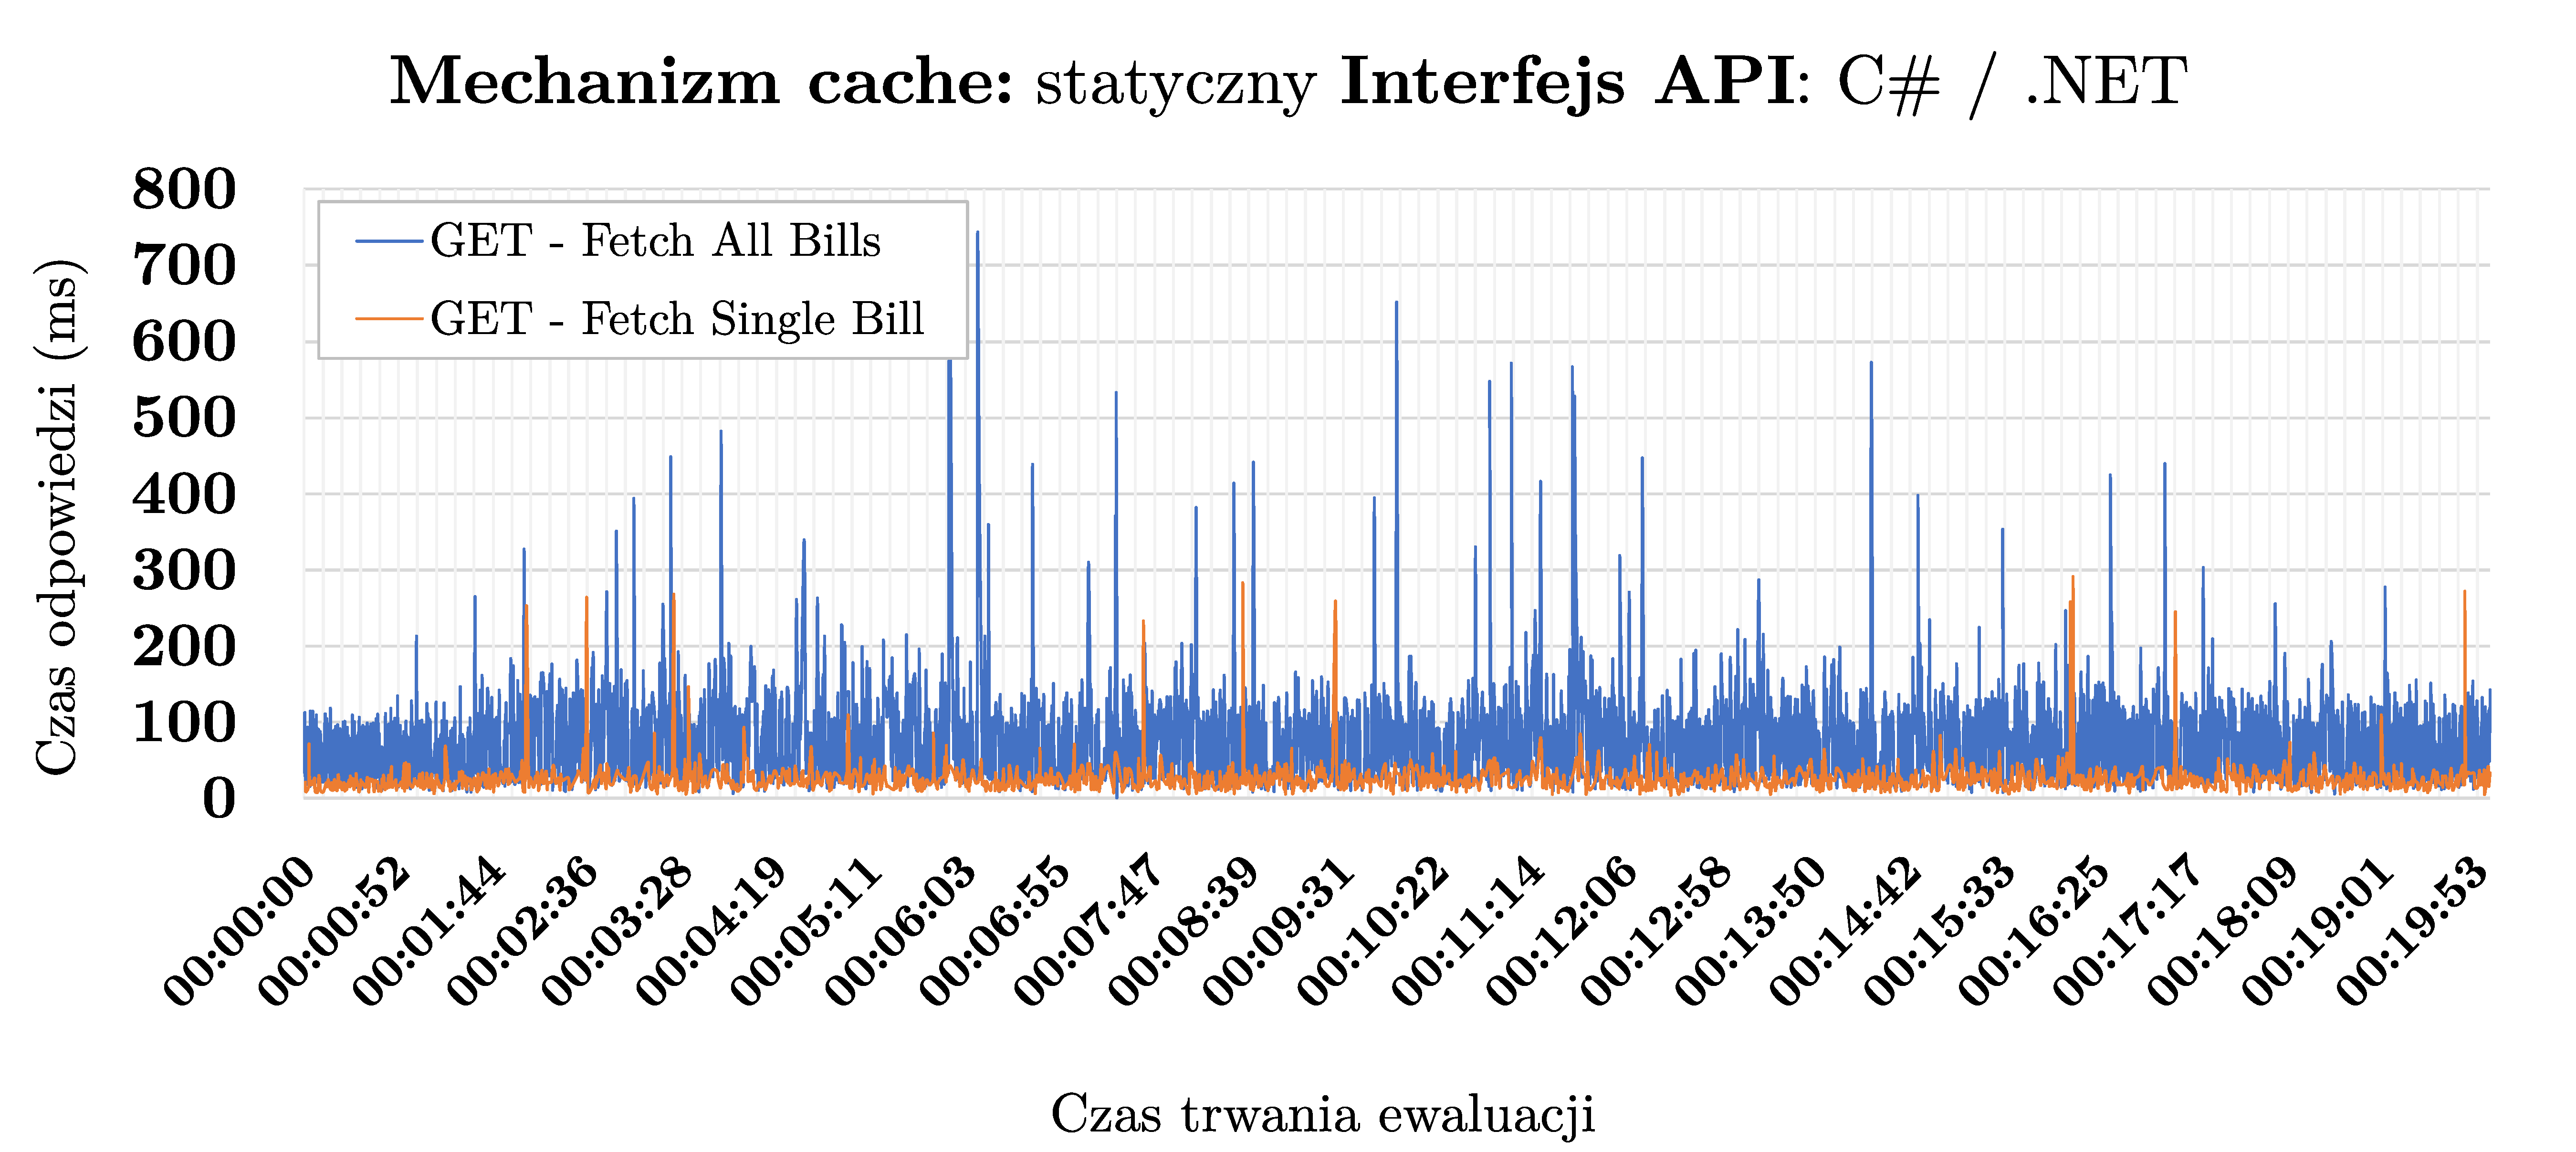
\includegraphics[width=0.49\textwidth]{rys05/dotnet-static-cache-chart.pdf} & 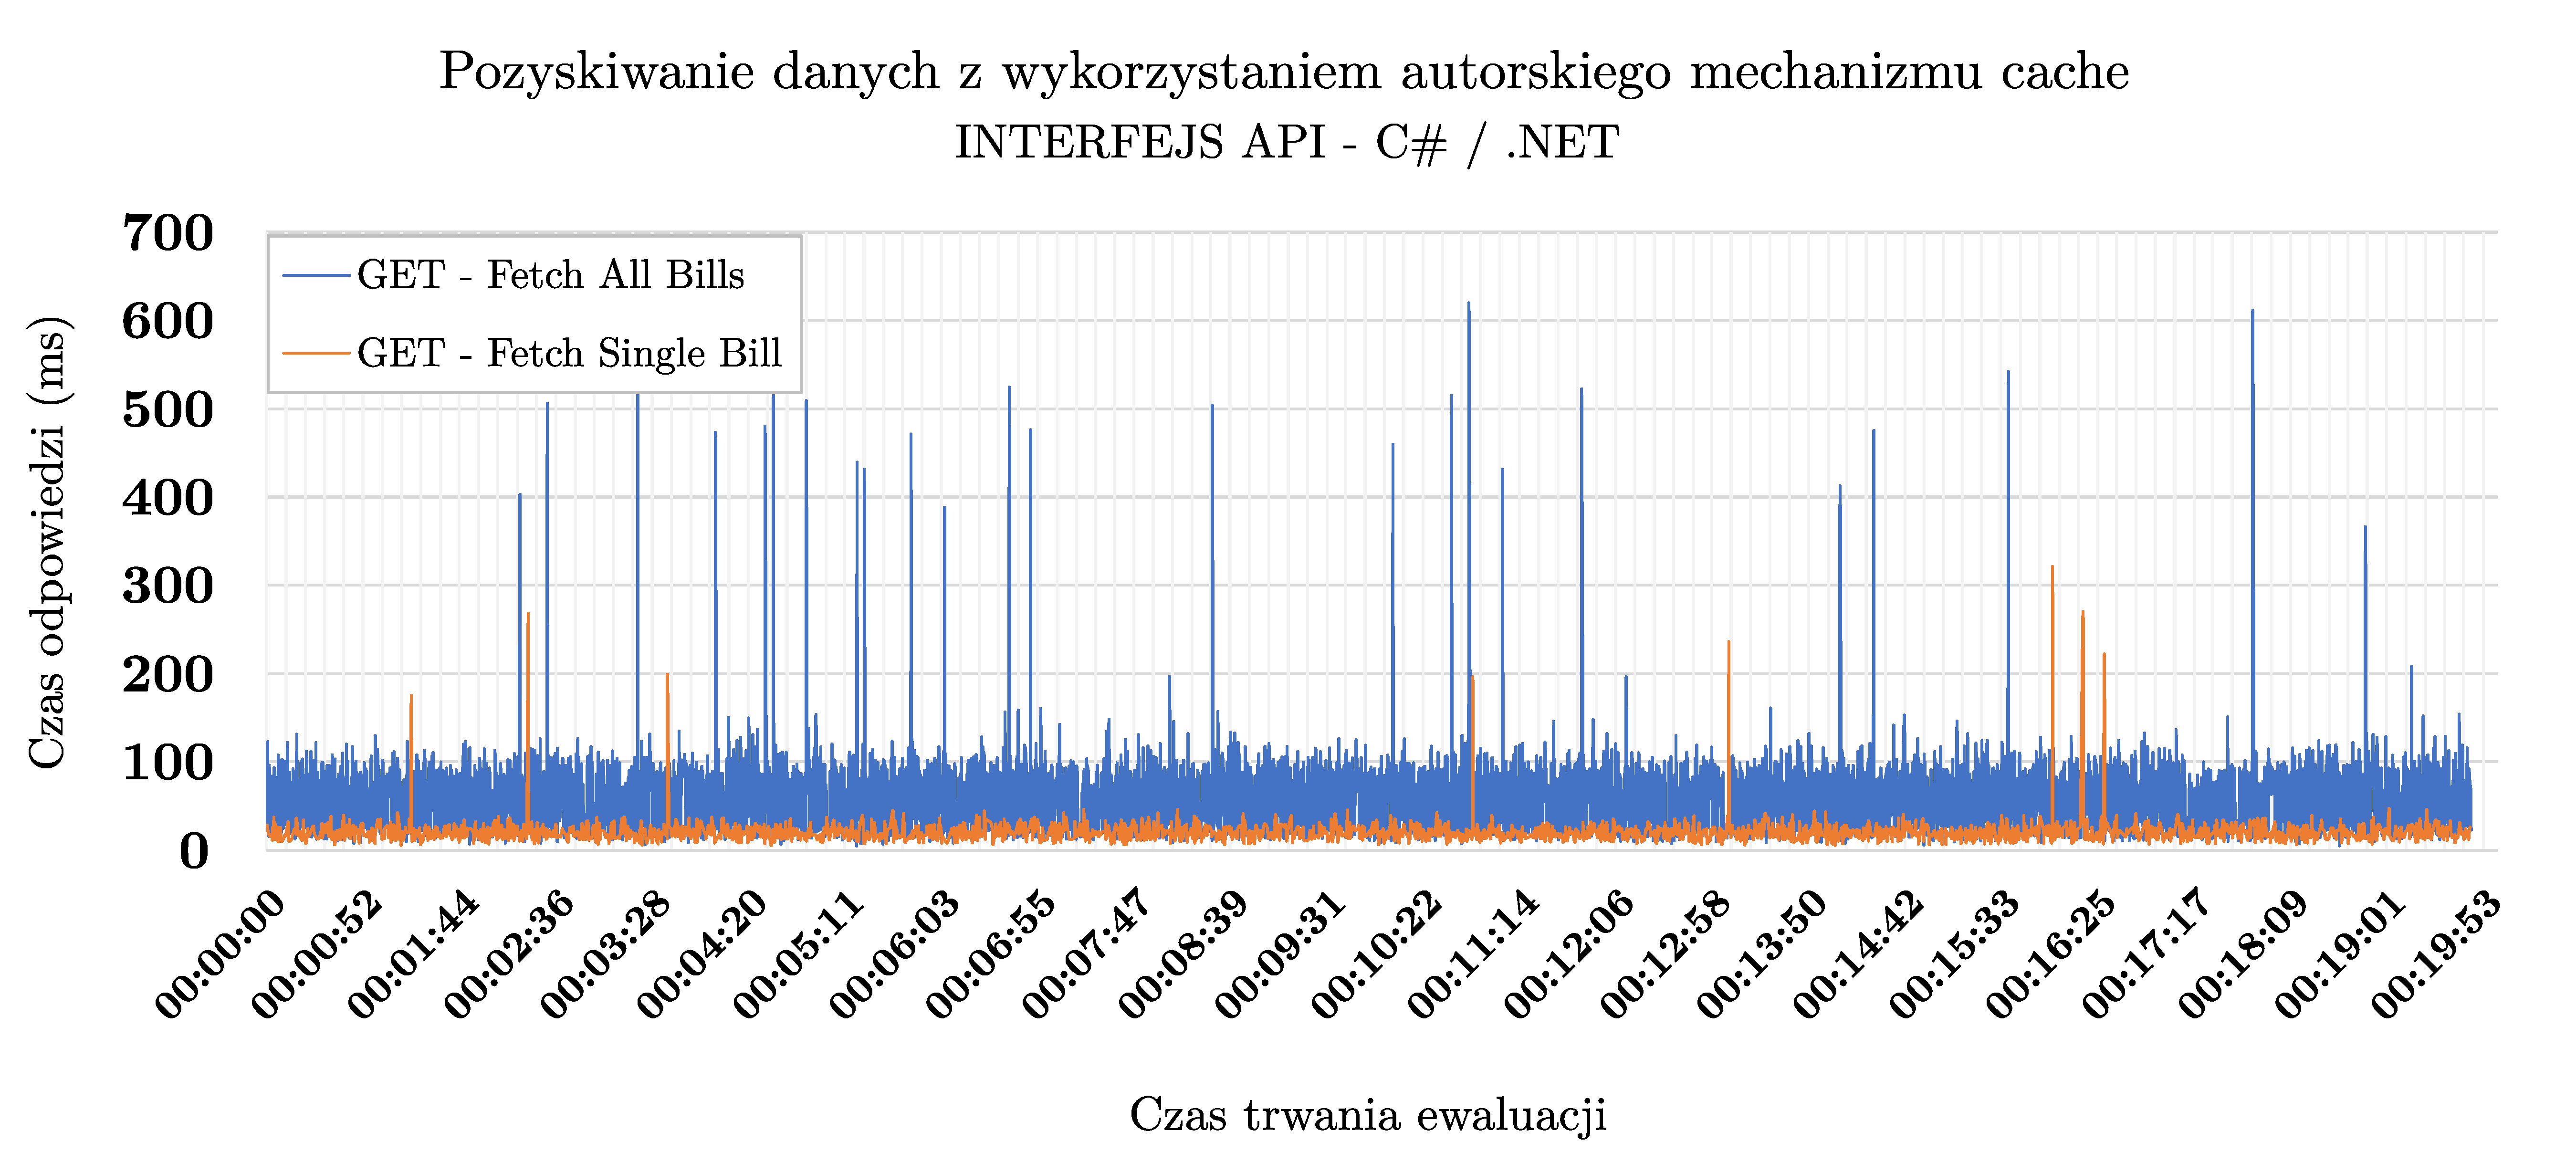
\includegraphics[width=0.49\textwidth]{rys05/dotnet-freq-cache-chart.pdf} \\
    c) & d) \\
    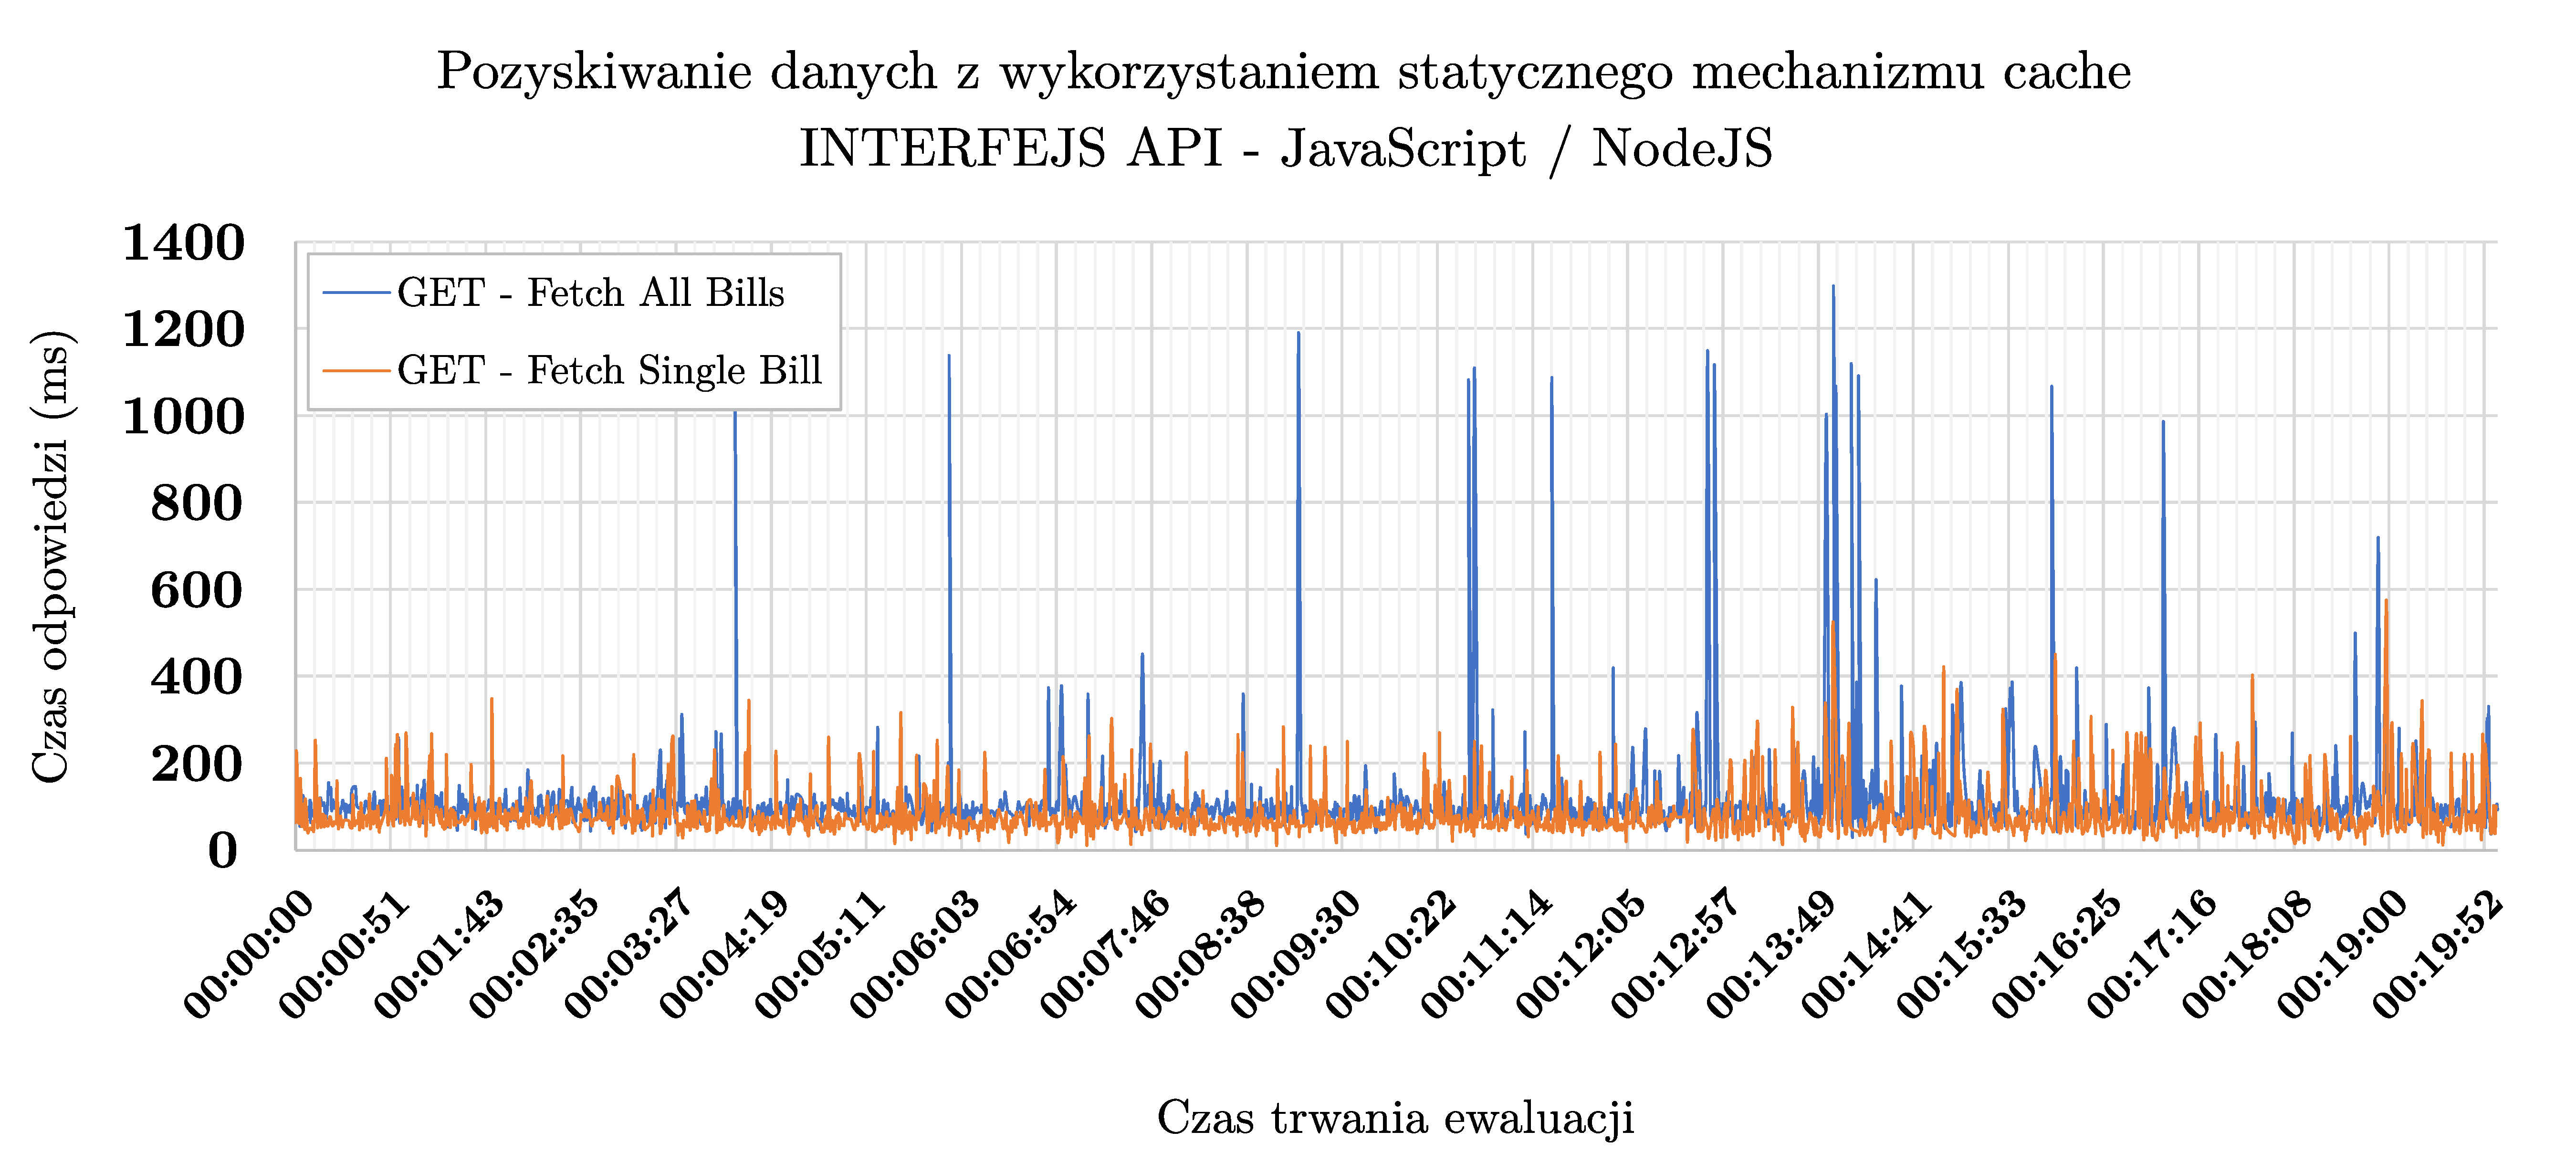
\includegraphics[width=0.49\textwidth]{rys05/nodejs-static-cache.pdf} & 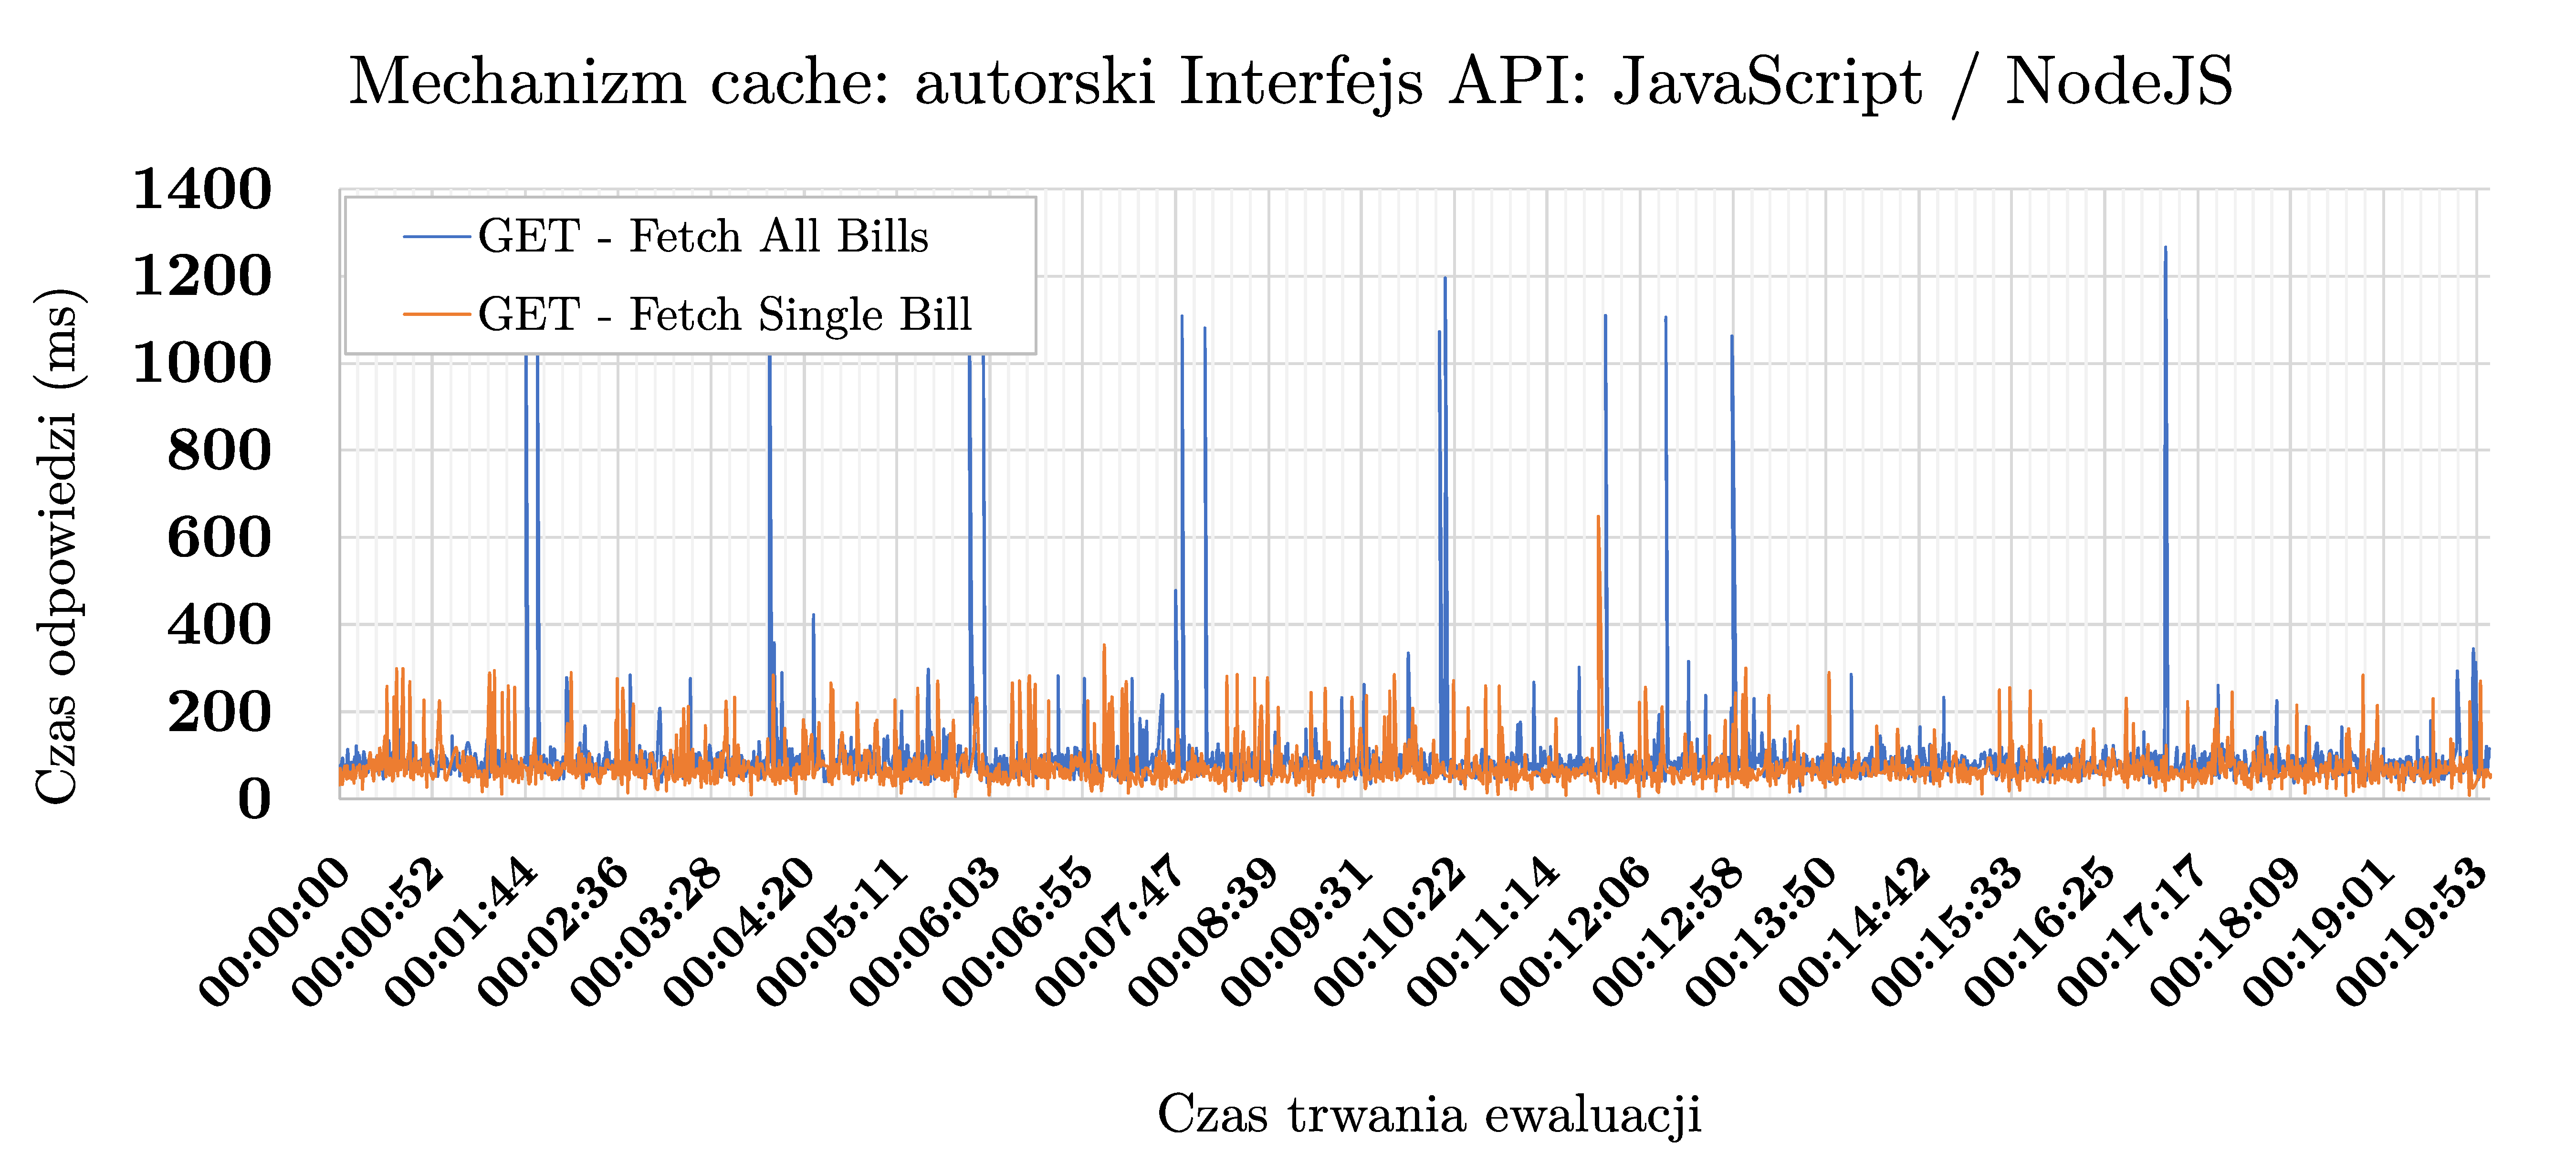
\includegraphics[width=0.49\textwidth]{rys05/nodejs-freq-cache.pdf}
    % jezeli obraki sa rownej wysokosci, mozna je wyrownac do gory stosujac vtop jak nizej
    % \vtop{\vskip-2ex\hbox{{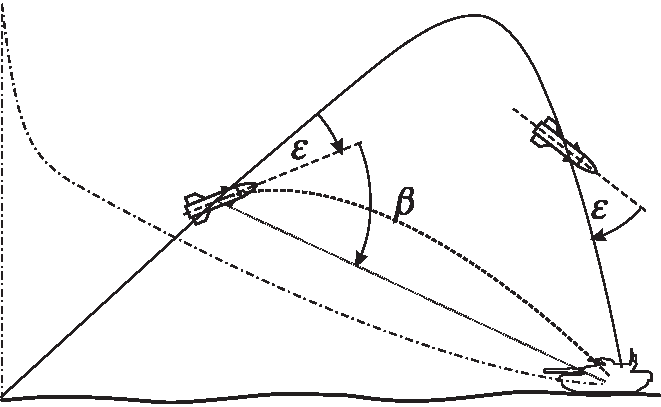
\includegraphics[width=0.475\textwidth]{rys05/beta1}}}} &
    % \vtop{\vskip-2ex\hbox{{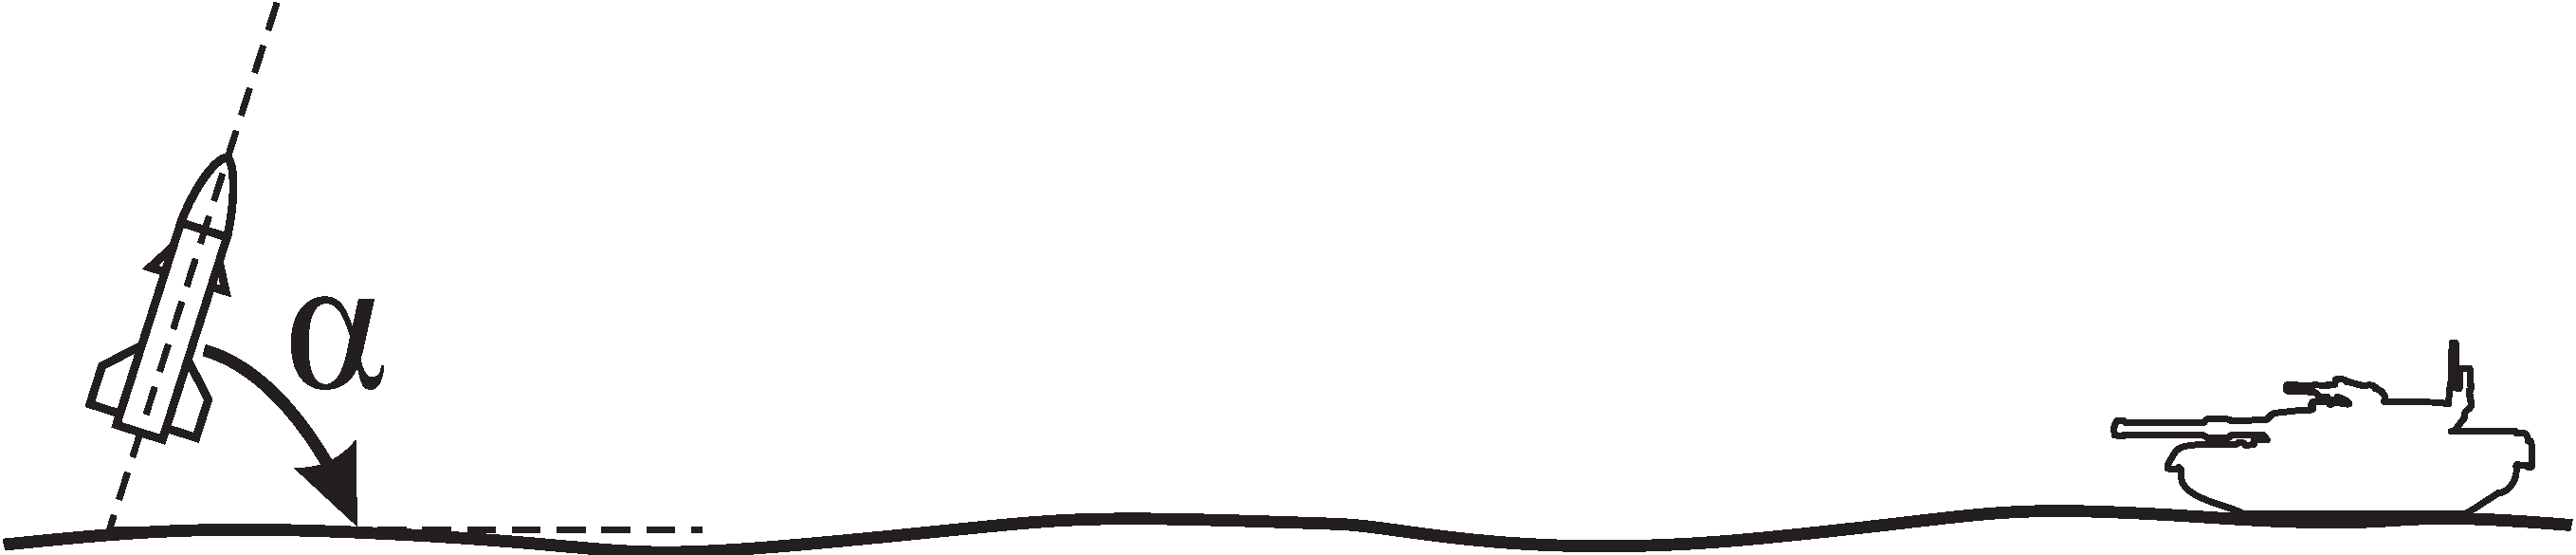
\includegraphics[width=0.475\textwidth]{rys05/alfa1}}}}  \caption{Wyznaczanie trajektorii lotu rakiety: 
    \end{tabular}
  \caption{Porównanie czasów odpowiedzi na żądanie dla odmiennych mechanizmów pamięci podręcznej}
  \label{fig:cache-charts}
\end{figure}

W kontekście interfejsu programowania aplikacji zaimplementowanego w języku C\# zauważyć możemy znaczące wydłużenie się przedziałów czasowych, w ramach których nie występują żądania o wysokim czasie odpowiedzi. Trend ten, nie jest jednakże tak dobrze dostrzegalny w odniesieniu eksperymentu przeprowadzanego z wykorzystaniem interfejsu API napisanego w JavaScript. Ponadto, niezależnie od technologii, nie jest zauważalne spodziewane, stopniowe rozszerzanie się odcinków niskich czasów odpowiedzi, wraz z postępem ewaluacji. Może to być spowodowane nieadekwatnymi wartościami liczników unieważnień, które określone zostały na podstawie poprzednich eksperymentów wykorzystujących mechanizm o stałym czasie przechowywania wpisu.
\section{Zmienność wydajności api wdrożonego na generycznej oraz dedykowanej platformie chmurowej}
Ostatnia ze zrealizowanych w ramach niniejszej pracy ewaluacji odnosi się do analizy zmiany wydajności pracy interfejsów programowania aplikacji w zależności od środowiska wdrożeniowego, w ramach którego usługa sieciowa jest hostowana. Celem niniejszego badania jest sprawdzenie, czy wykorzystanie dedykowanej rozwiązaniu platformy chmurowej, pozwala na uzyskanie lepszych rezultatów działania api, niż w przypadku wdrożenia systemu internetowego na infrastrukturze generycznej, którą jest wirtualny serwer prywatny.

Zdecydowano się na zastosowanie usługi w modelu infrastructure-as-a-service, która pełniła rolę środowiska produkcyjnego niezależnego od technologii implementacji api. W środowisku tym, wdrożono interfejsy programowania aplikacji napisane w językach C\# oraz JavaScript, wykorzystując serwer HTTP Apache oraz usługę odwróconego proxy. Ponadto, każda z poddawanych analizie usług, komunikowała się z silnikiem bazodanowym znajdującym się wewnątrz wirtualnego serwera prywatnego. Dzięki temu, wyeliminiować można było zjawisko zmienności czasu połączenia pomiędzy interfejsem a źródłem danych, która to zmienność wynika z niedeterministycznego charakteru łącza sieciowego. Aby zachować pełną generyczność omawianego rozwiązania zastosowano jeden z najpopularniejszych systemów bazodanowych jakim jest MySQL. System ten, choć w znaczącym stopniu wspierany przez aplikacje tworzone w językach C\# oraz JavaScript, nie jest rozwiązaniem postrzeganym jako dedykowane względem platform .NET oraz NodeJS. 

Jako podejścia referencyjne względem infrastruktury generycznej, wdrożone zostały interfejsy programowania aplikacji na platformach Microsoft Azure oraz Heroku. Pierwsza z nich, jest usługą dedykowaną dla rozwiązań bazujących na platformie .NET oraz napisanych w języku C\#. W tym przypadku, interfejs programowania aplikacji połączono z bazą danych Microsoft SQL Server. Druga z platform to rekomendowane rozwiązanie dla systemów internetowych tworzonych z wykorzystaniem środowiska uruchomieniowego NodeJS. Interfejs API wdrożony na platformie Heroku, skomunikowany został z nierelacyjną bazą danych MongoDB.

Odnosząc się do metryk gromadzonych w ramach niniejszego badania, wspomnieć należy o fakcie, że rezultaty wykonywanych operacji nie stanowią wartości czasu odpowiedzi na żądanie, a jedynie czas przetwarzania zapytania wewnątrz metody kontrolera interfejsu programowania aplikacji. Takie podejście, pozwala na uniezależnienie ewaluacji względem lokalizacji oraz szybkości łącza internetowego urządzeń generujących zapytania.

W przeprowadzonym badaniu generowano zapytania pod pięć punktów końcowych, które wykorzystywane były również w eksperymencie \ref{research:crud}. Ich szczegółowa charakterystyka zawarta została w tabeli \ref{tab:endpointy-scenario-1}. Przed rozpoczęciem analizy, zestawiono rozproszoną konfigurację topologii fizycznej nr 5, która opisana została w sekcji \ref{sec:rozproszone-srodowisko-badawcze-ver-1}, a także dokonano ewaluacji funkcjonalnej zaimplementowanych rozwiązań, poprzez realizację testów linii bazowej. Plan testowy obejmował uruchomienie 40 współbieżnie pracujących wątków oprogramowania Apache JMeter, które generowały ruch sieciowy przez 10 minut. Całość badania była przeprowadzona zgodnie ze zdefiniowanym uprzednio scenariuszem badawczym \ref{tab:research-scenario-6}.

Kluczowymi wskaźnikami wydajności rozwiązań wdrażanych na platformach chmurowych są: czas realizacji pojedynczego zapytania, procent błędnych odpowiedzi w kontekście poprawnych zapytań, a także efektywność wykorzystania zasobów fizycznego sprzętu. Zdecydowano się na pominięcie ostatniego z przytoczonych wskaźników, ponieważ w odniesieniu do tak przygotowanego badania, nie dostarcza on informacji, które mogłaby być przesłanką do formułowania jakichkolwiek hipotez dotyczących omawianego problemu. W czasie generowania zapytań w kierunku interfejsów programowania aplikacji, niezależnie od platform wdrożeniowych oraz uruchomieniowych, konsumpcja fizycznych zasobów sprzętowych cechowała się relatywną stałością w czasie. Oznacza to, że każda z poddawanych analizie platform chmurowych, jest w stanie obsłużyć znacząco większy ruch, niż ten, generowanych w ramach tego badania. Przeanalizowano natomiast, zarówno czas przetwarzania zapytania wewnątrz interfejsu, jak i liczbę błędnych zapytań w stosunku do wszystkich wygenerowanych.     

Na wykresach \ref{fig:dotnet-azure-vs-digitalocean} a) do \ref{fig:dotnet-azure-vs-digitalocean} h) zawarto porównanie rezultatów pozyskanych w czasie ewaluacji interfejsu programowania aplikacji napisanego w języku C\# i uruchamianego na platformach: generycznej (tj. DigitalOcean VPS), oraz dedykowanej (tj. Microsoft Azure).

\begin{figure}[htb]
  \centering
	\begin{tabular}{@{}ll@{}}
    a) & b) \\
    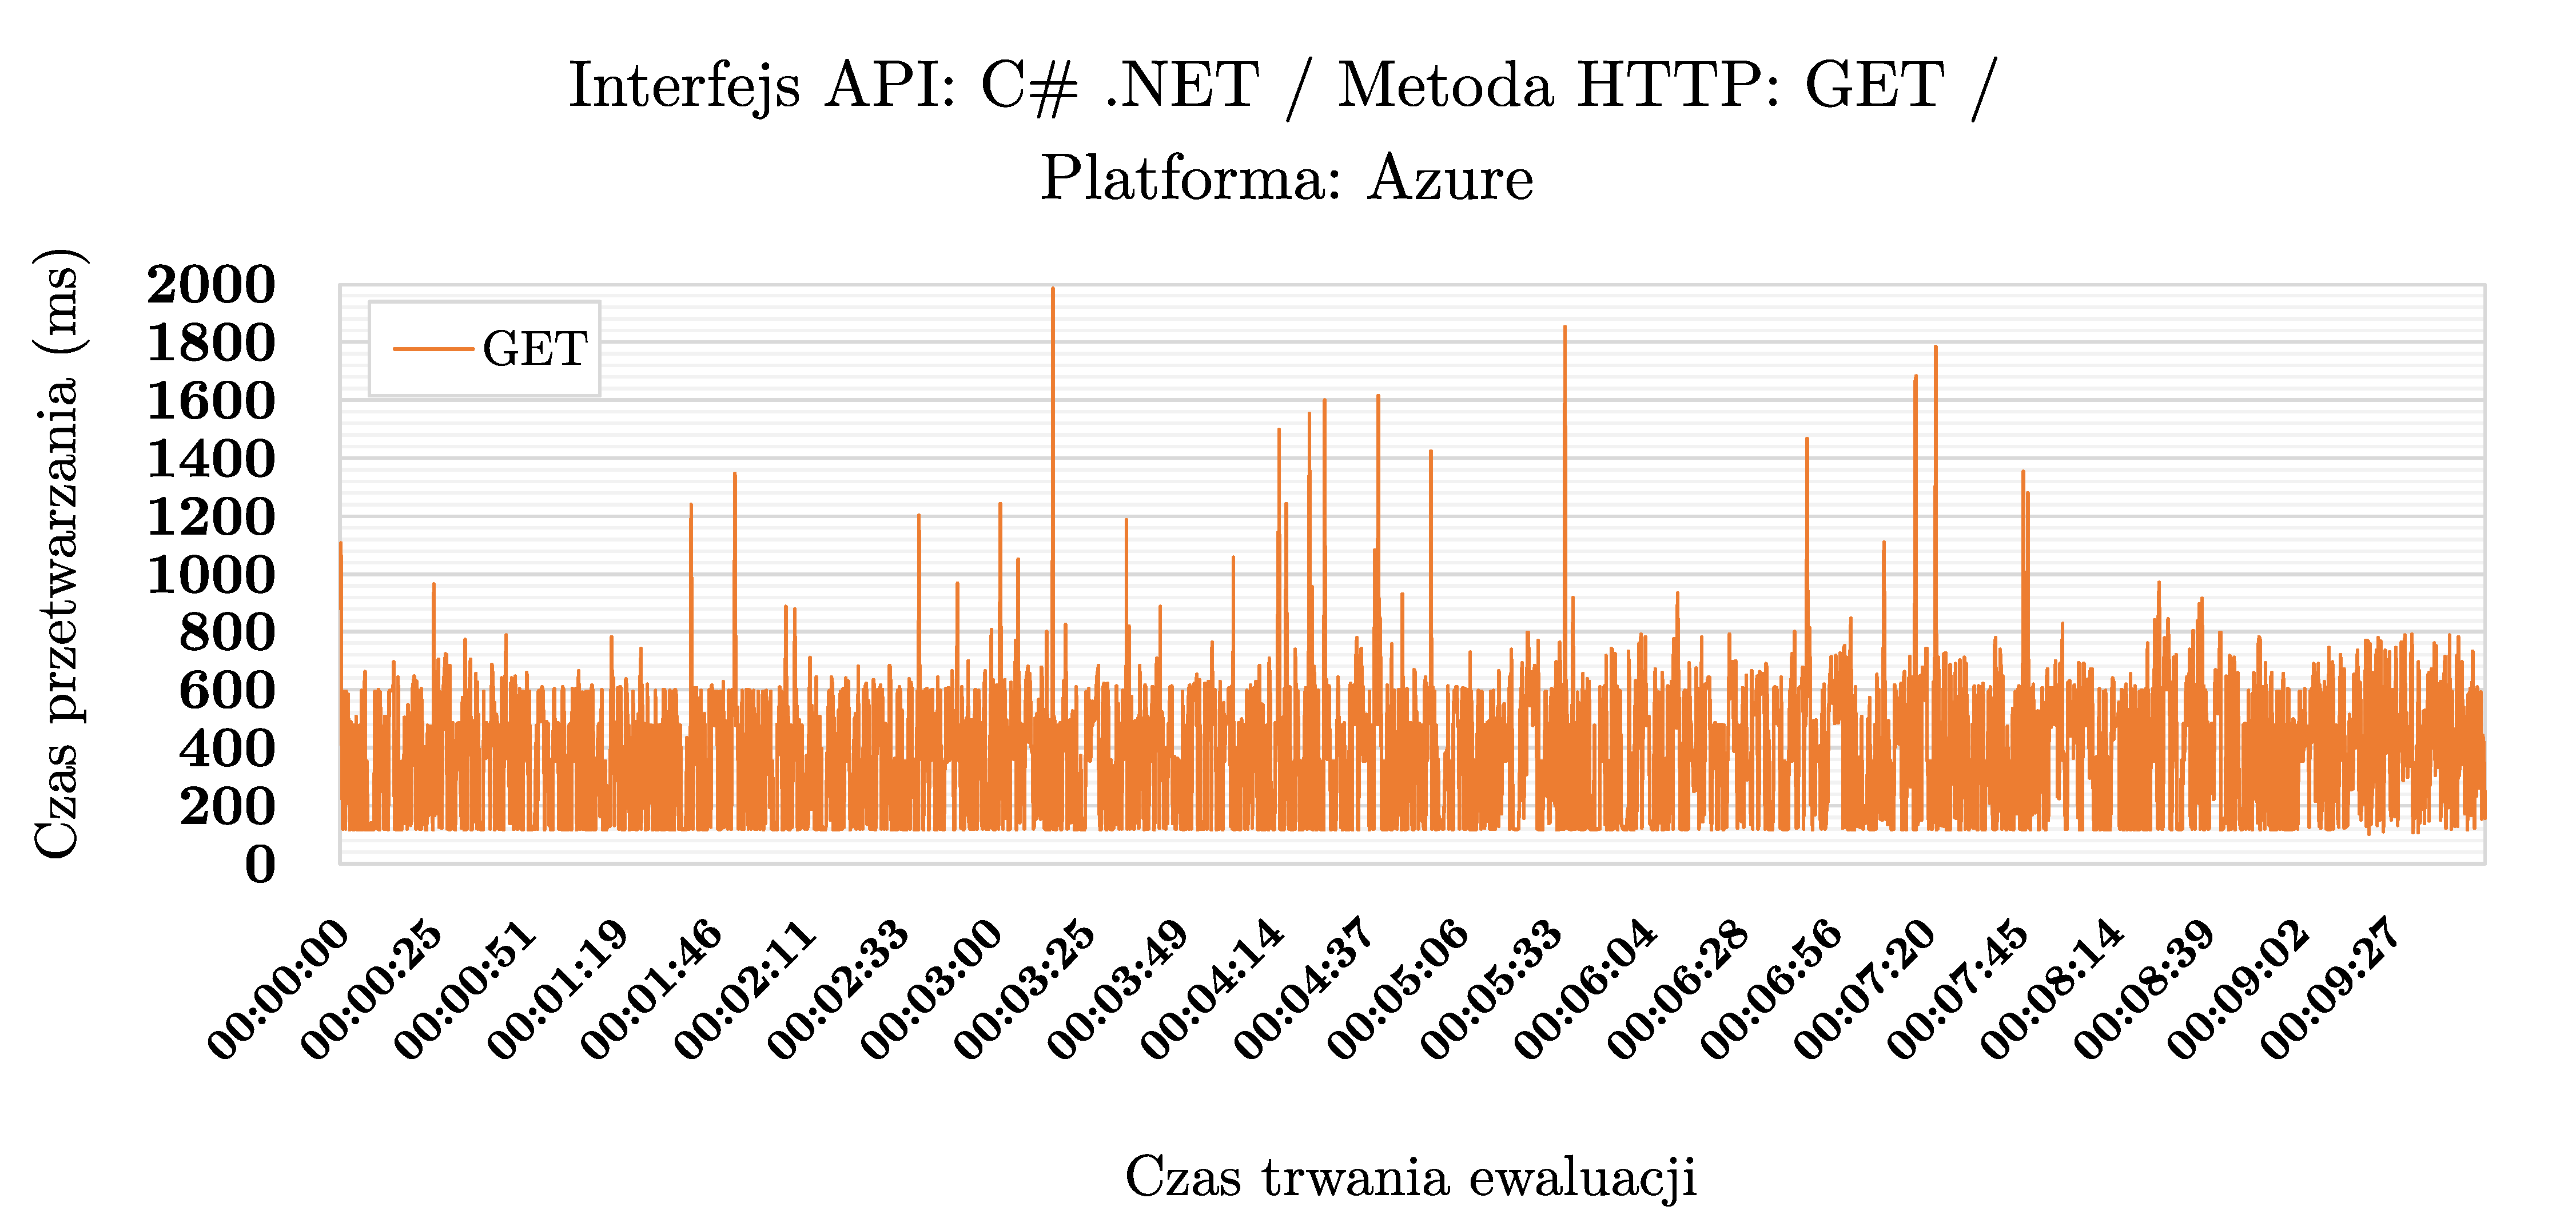
\includegraphics[width=0.49\textwidth]{rys05/dotnet-get-azure.pdf} & 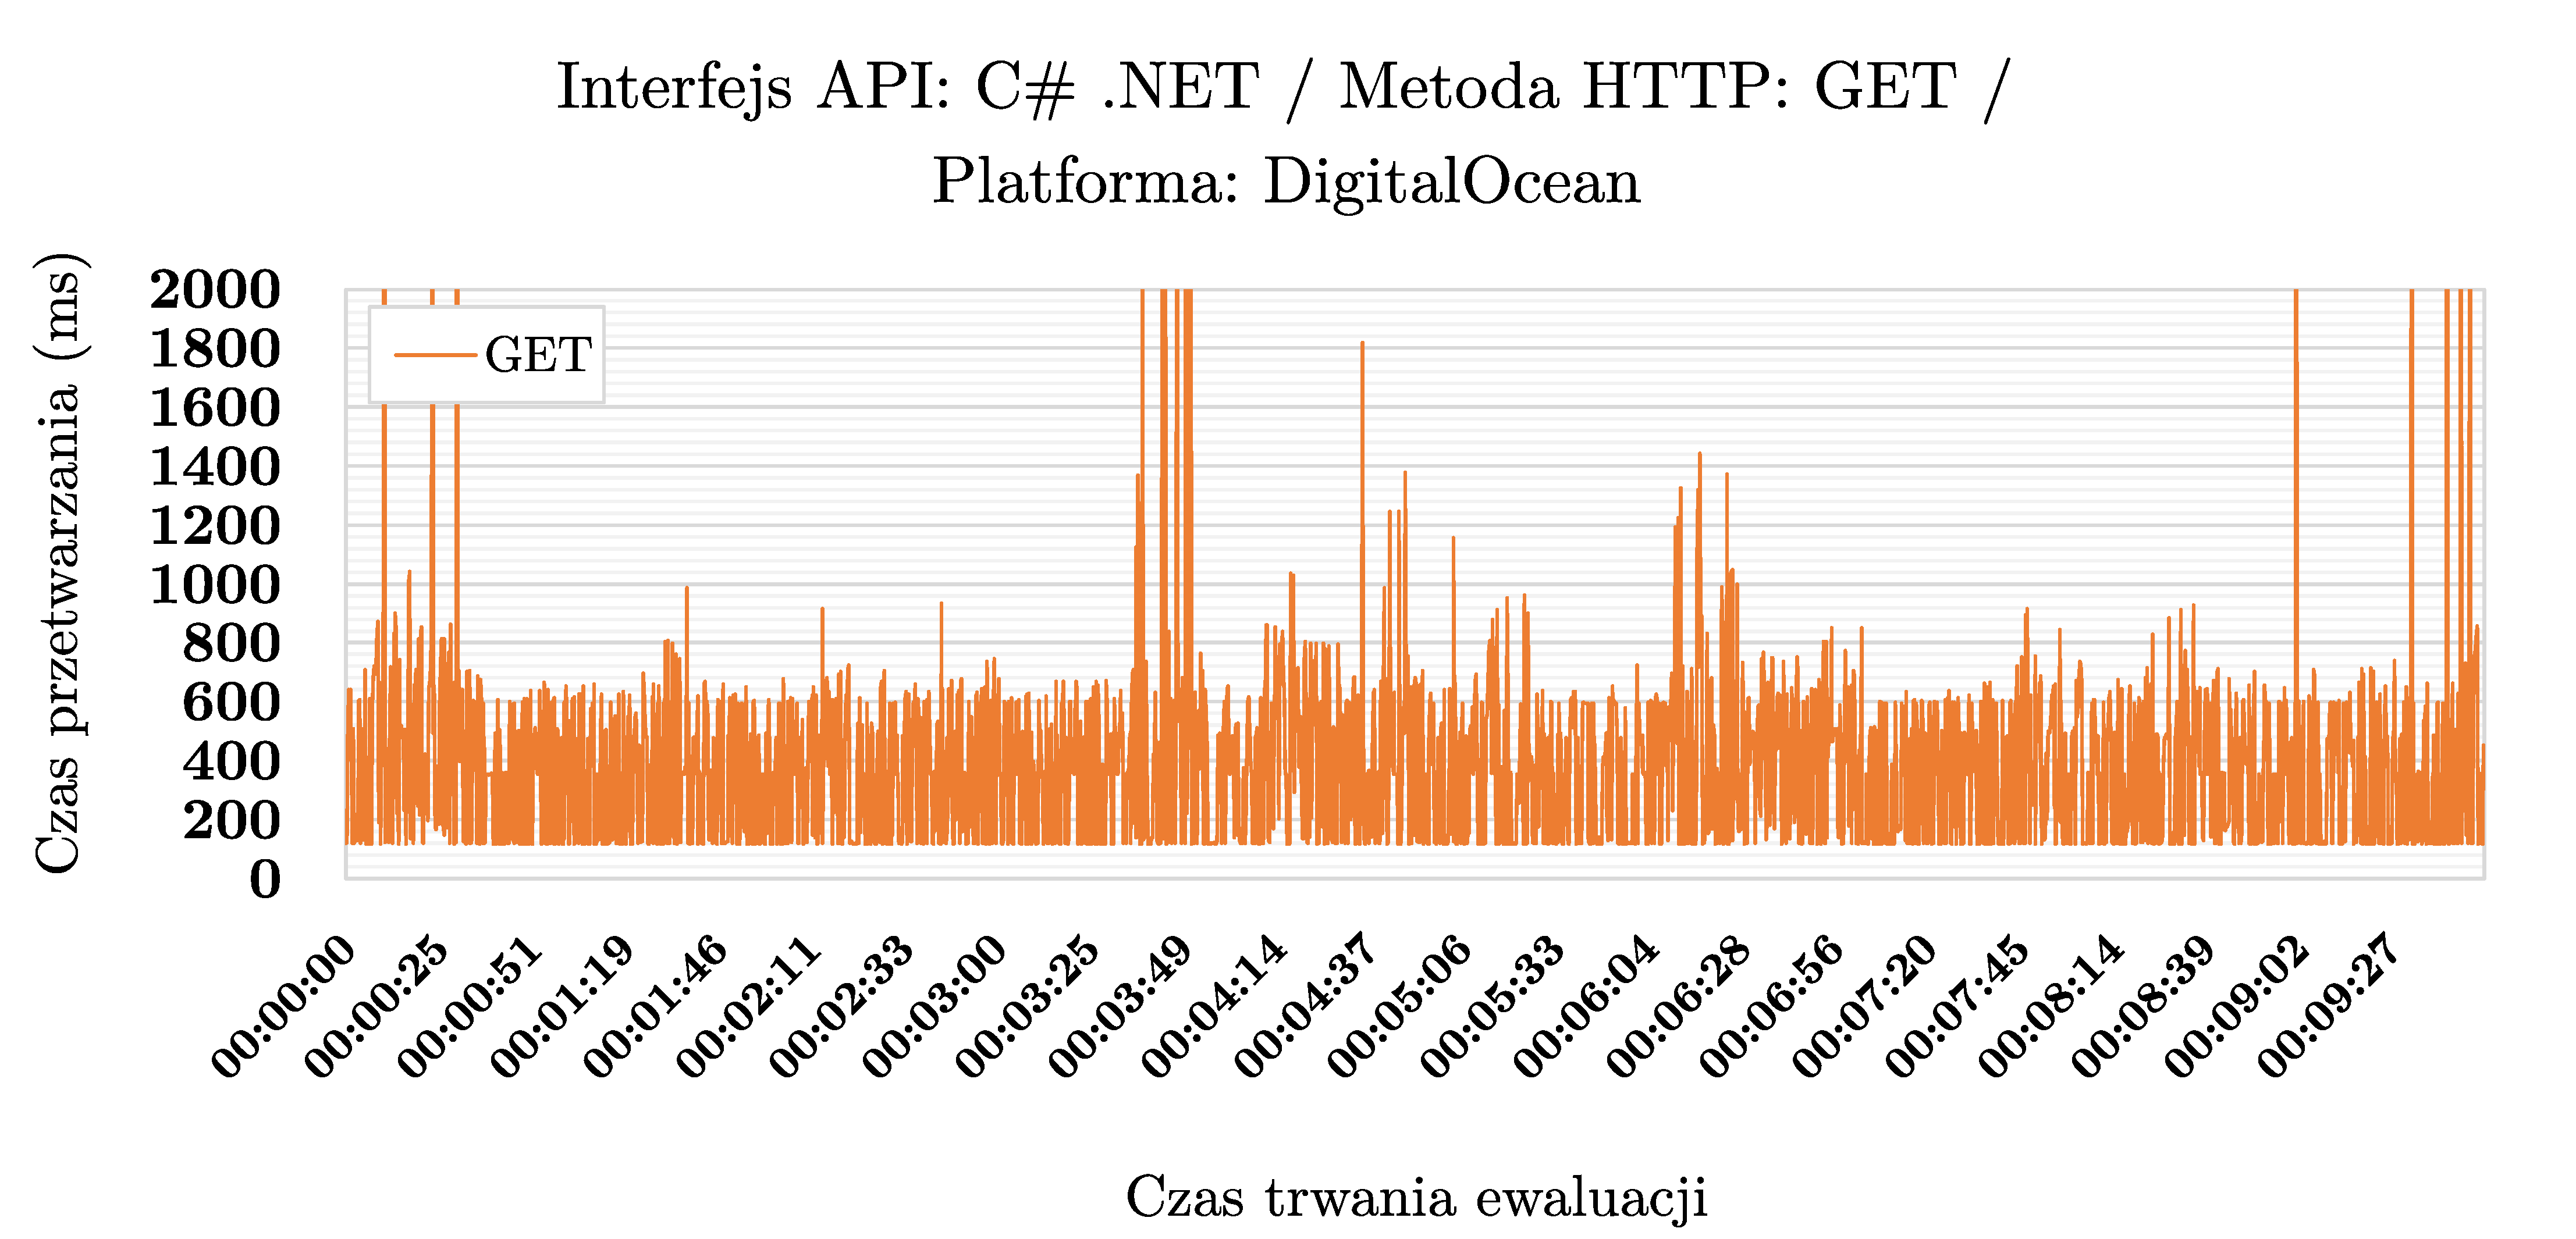
\includegraphics[width=0.49\textwidth]{rys05/dotnet-get-digitalocean.pdf} \\
    c) & d) \\
    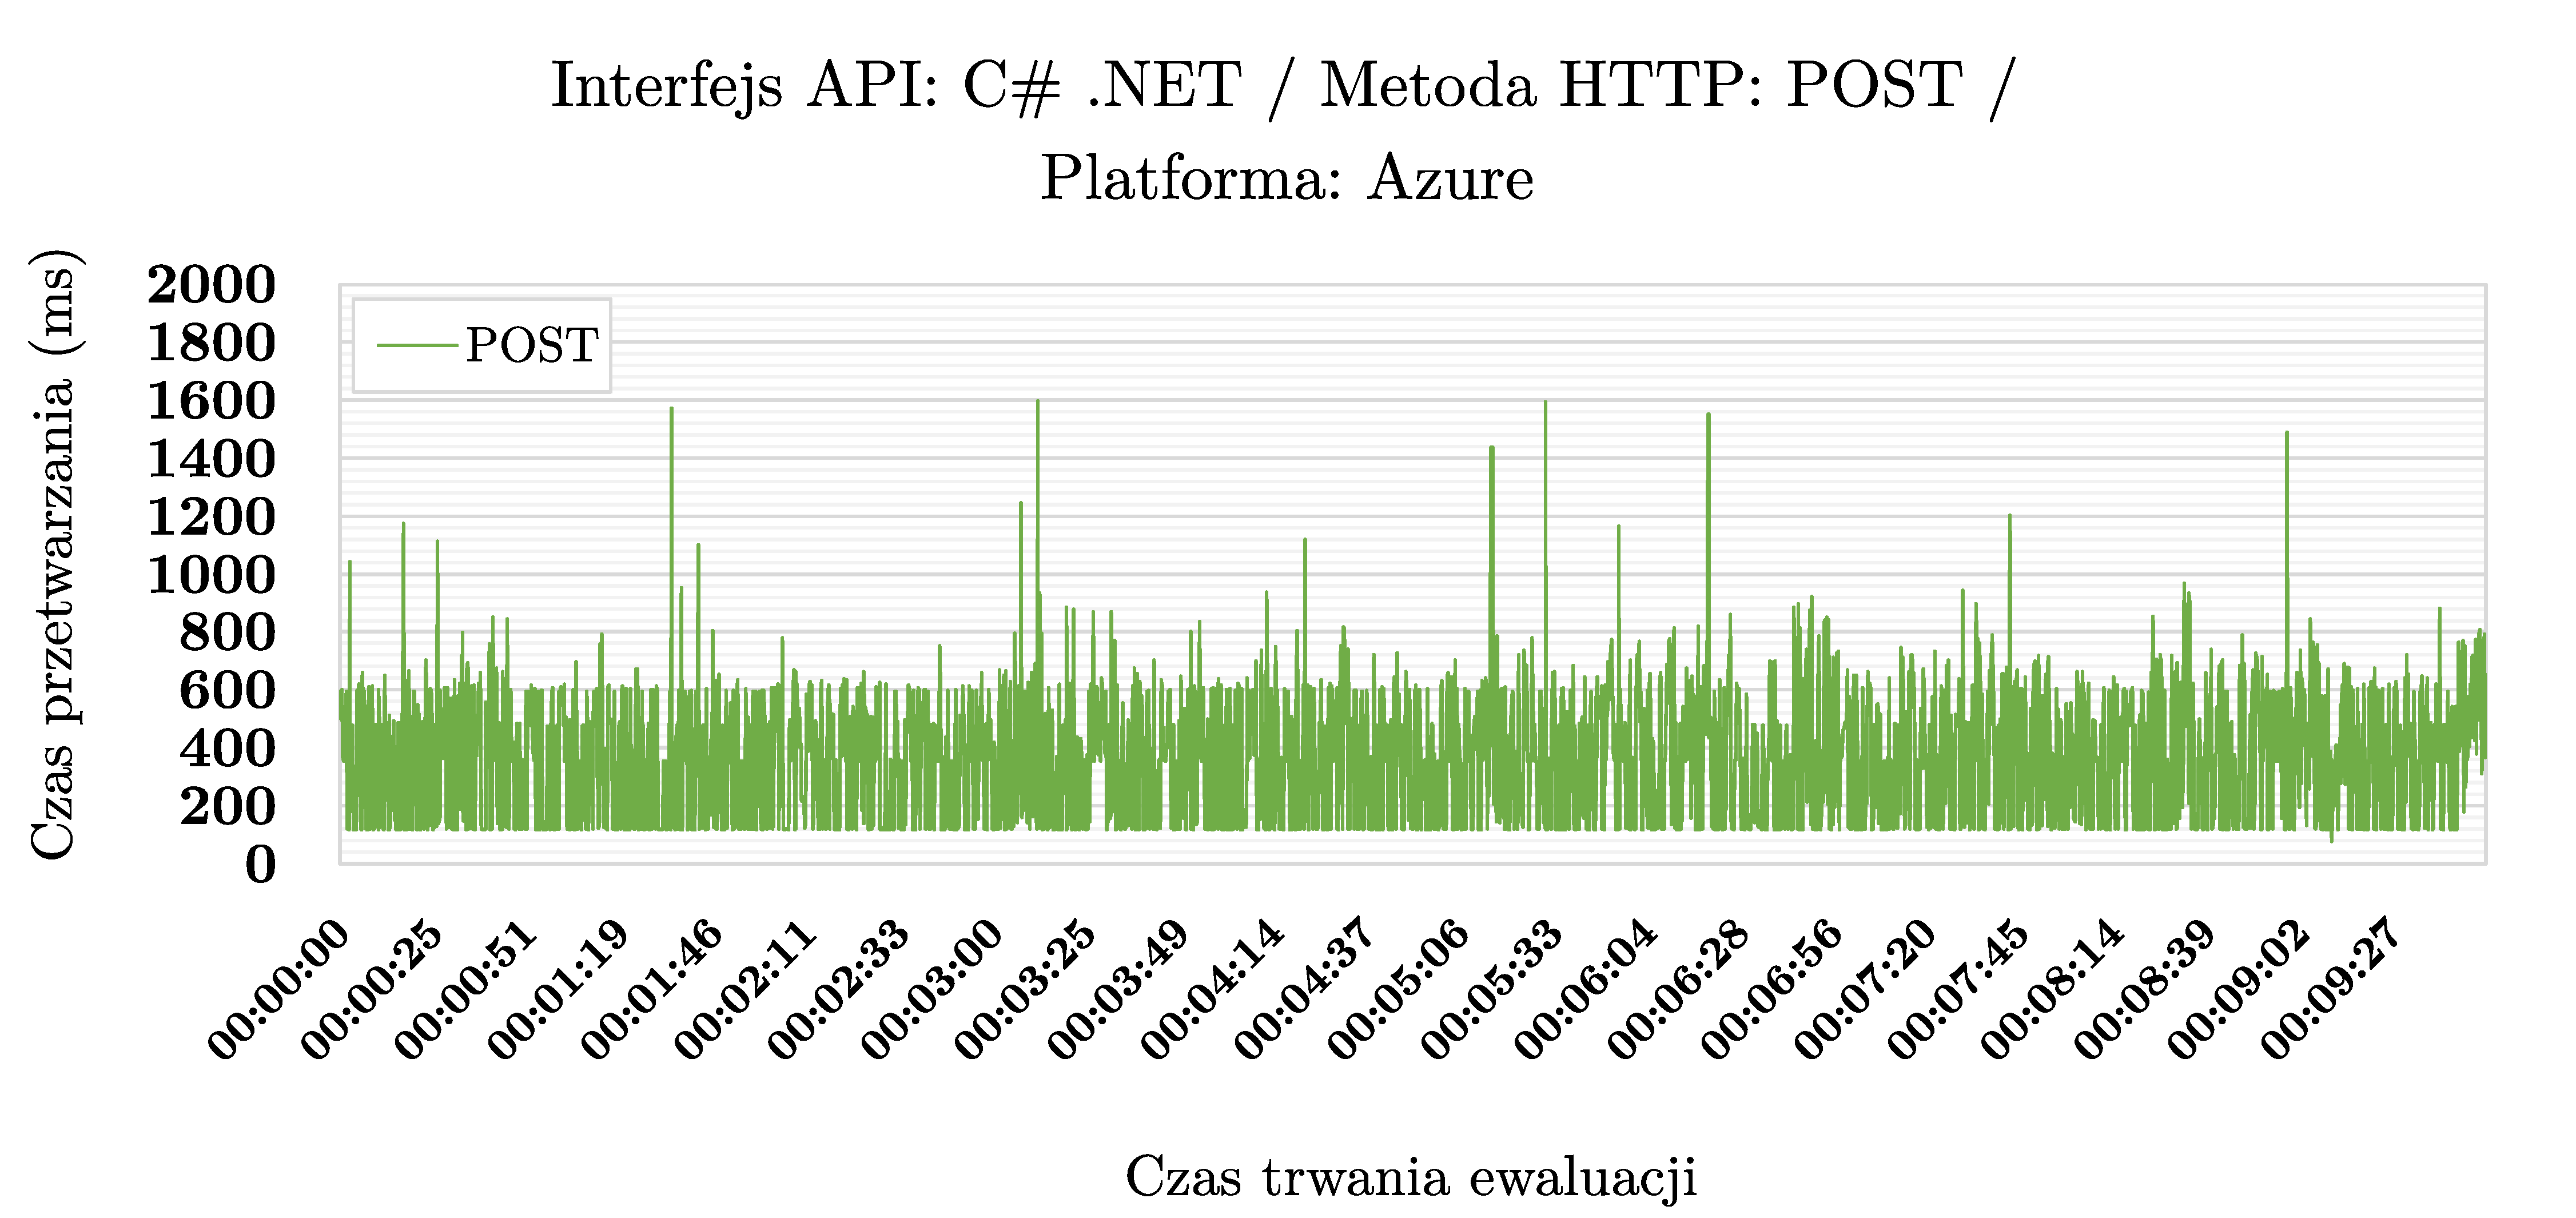
\includegraphics[width=0.49\textwidth]{rys05/dotnet-post-azure.pdf} & 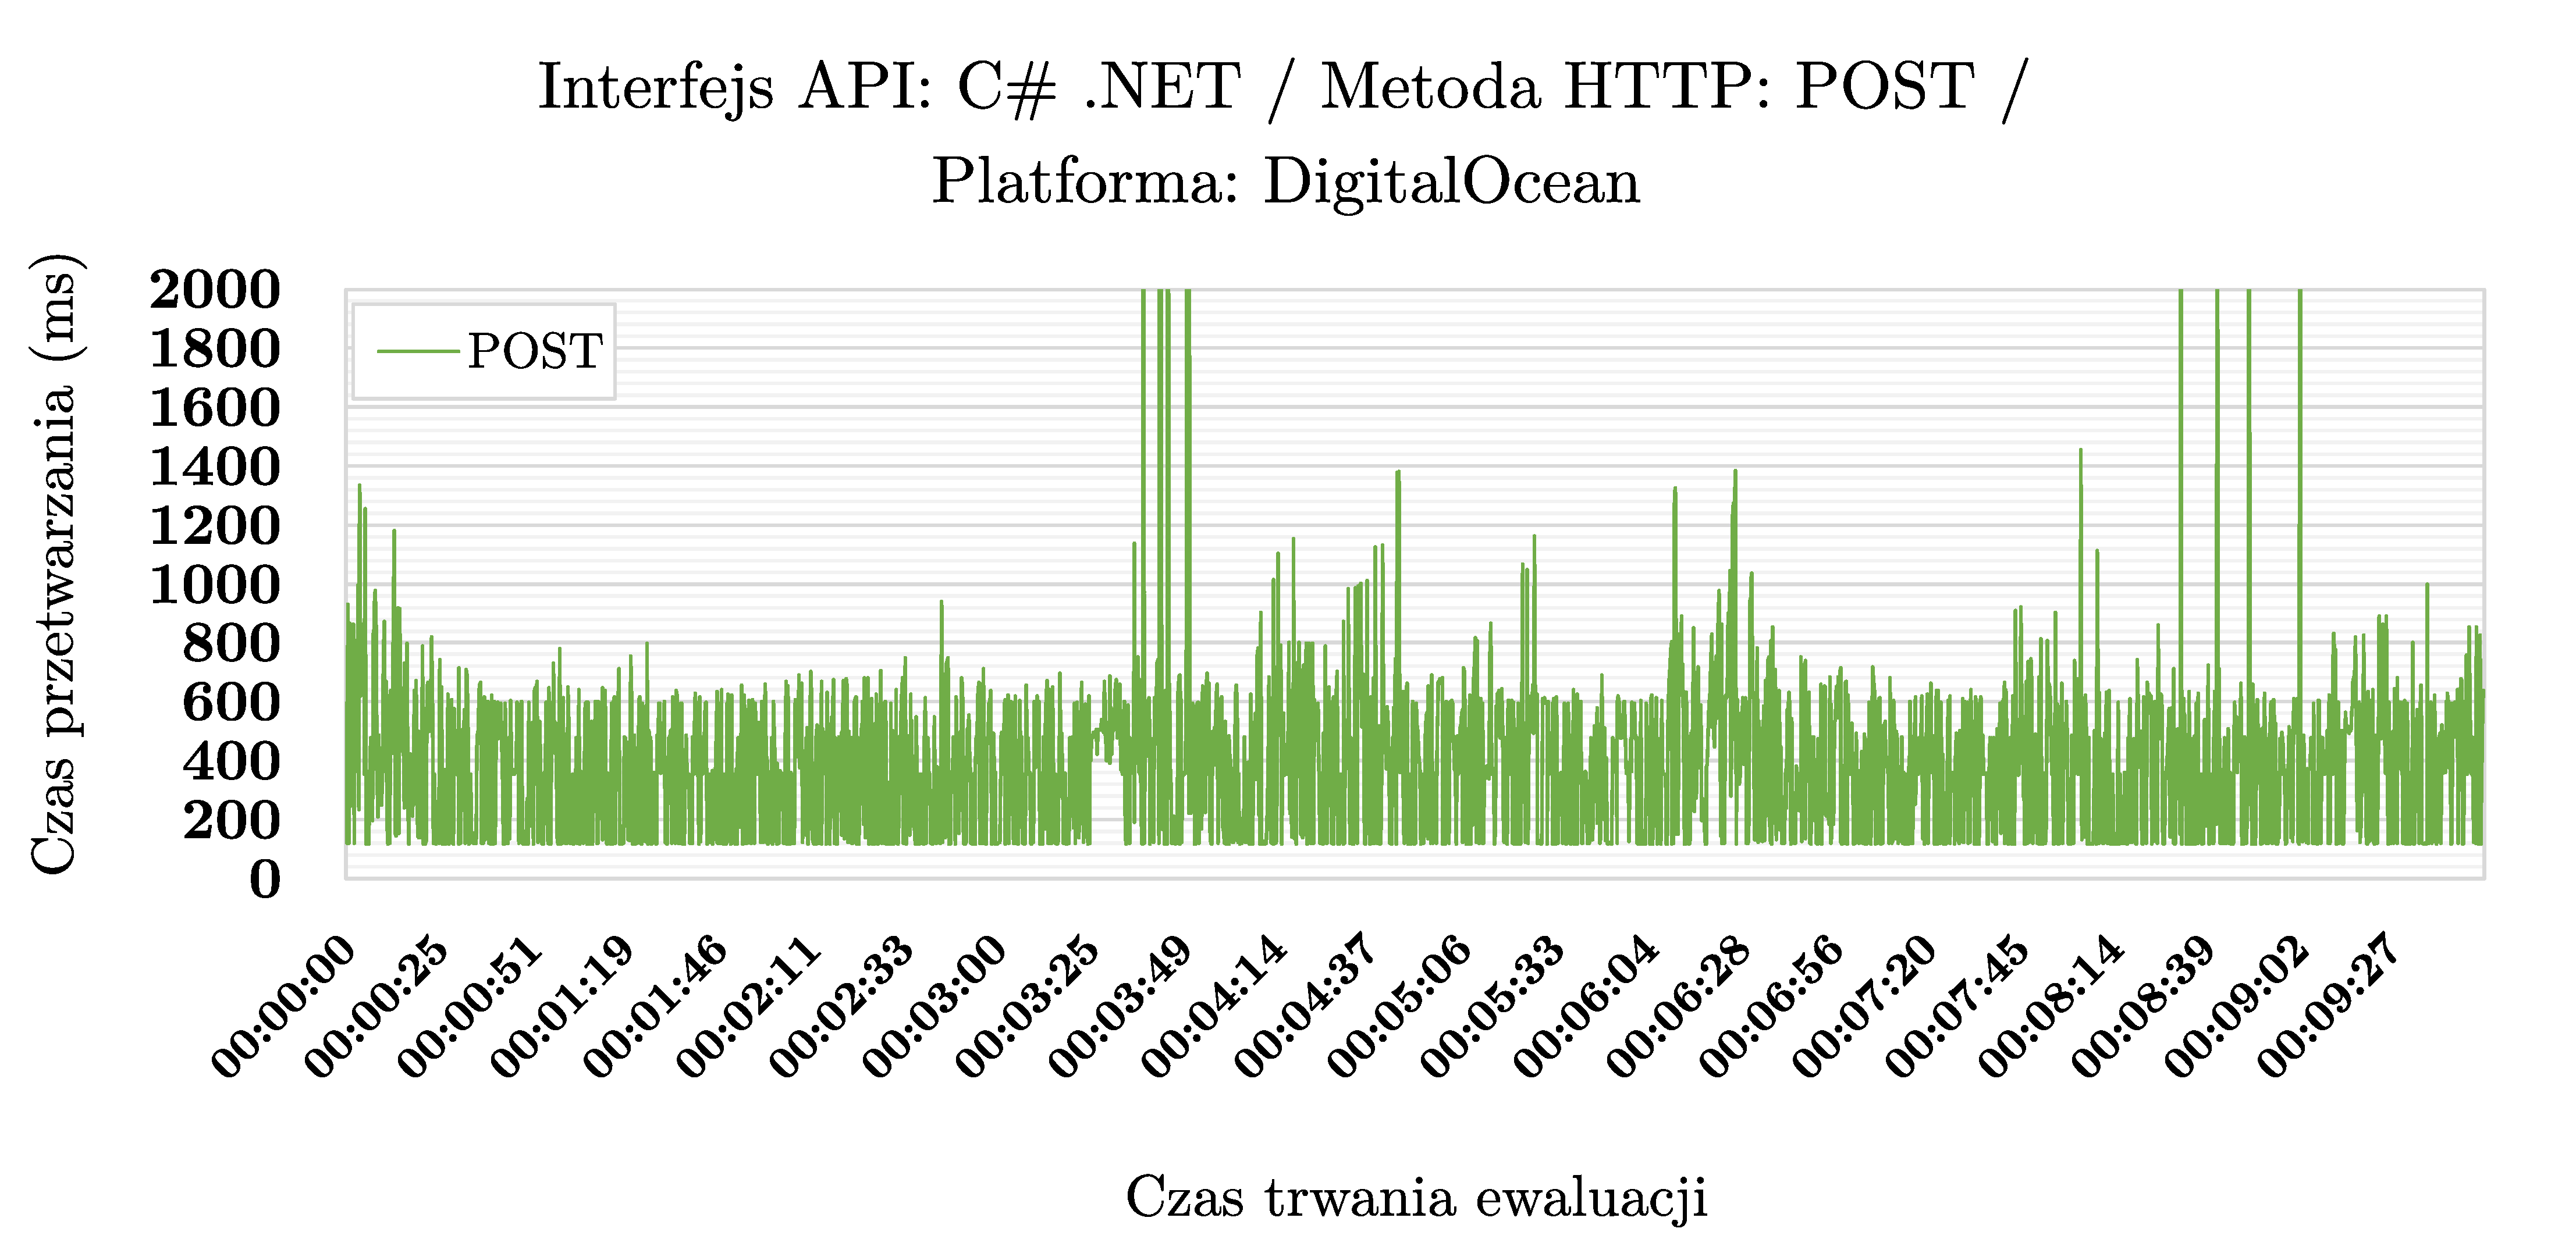
\includegraphics[width=0.49\textwidth]{rys05/dotnet-post-digitalocean.pdf} \\
    e) & f) \\
    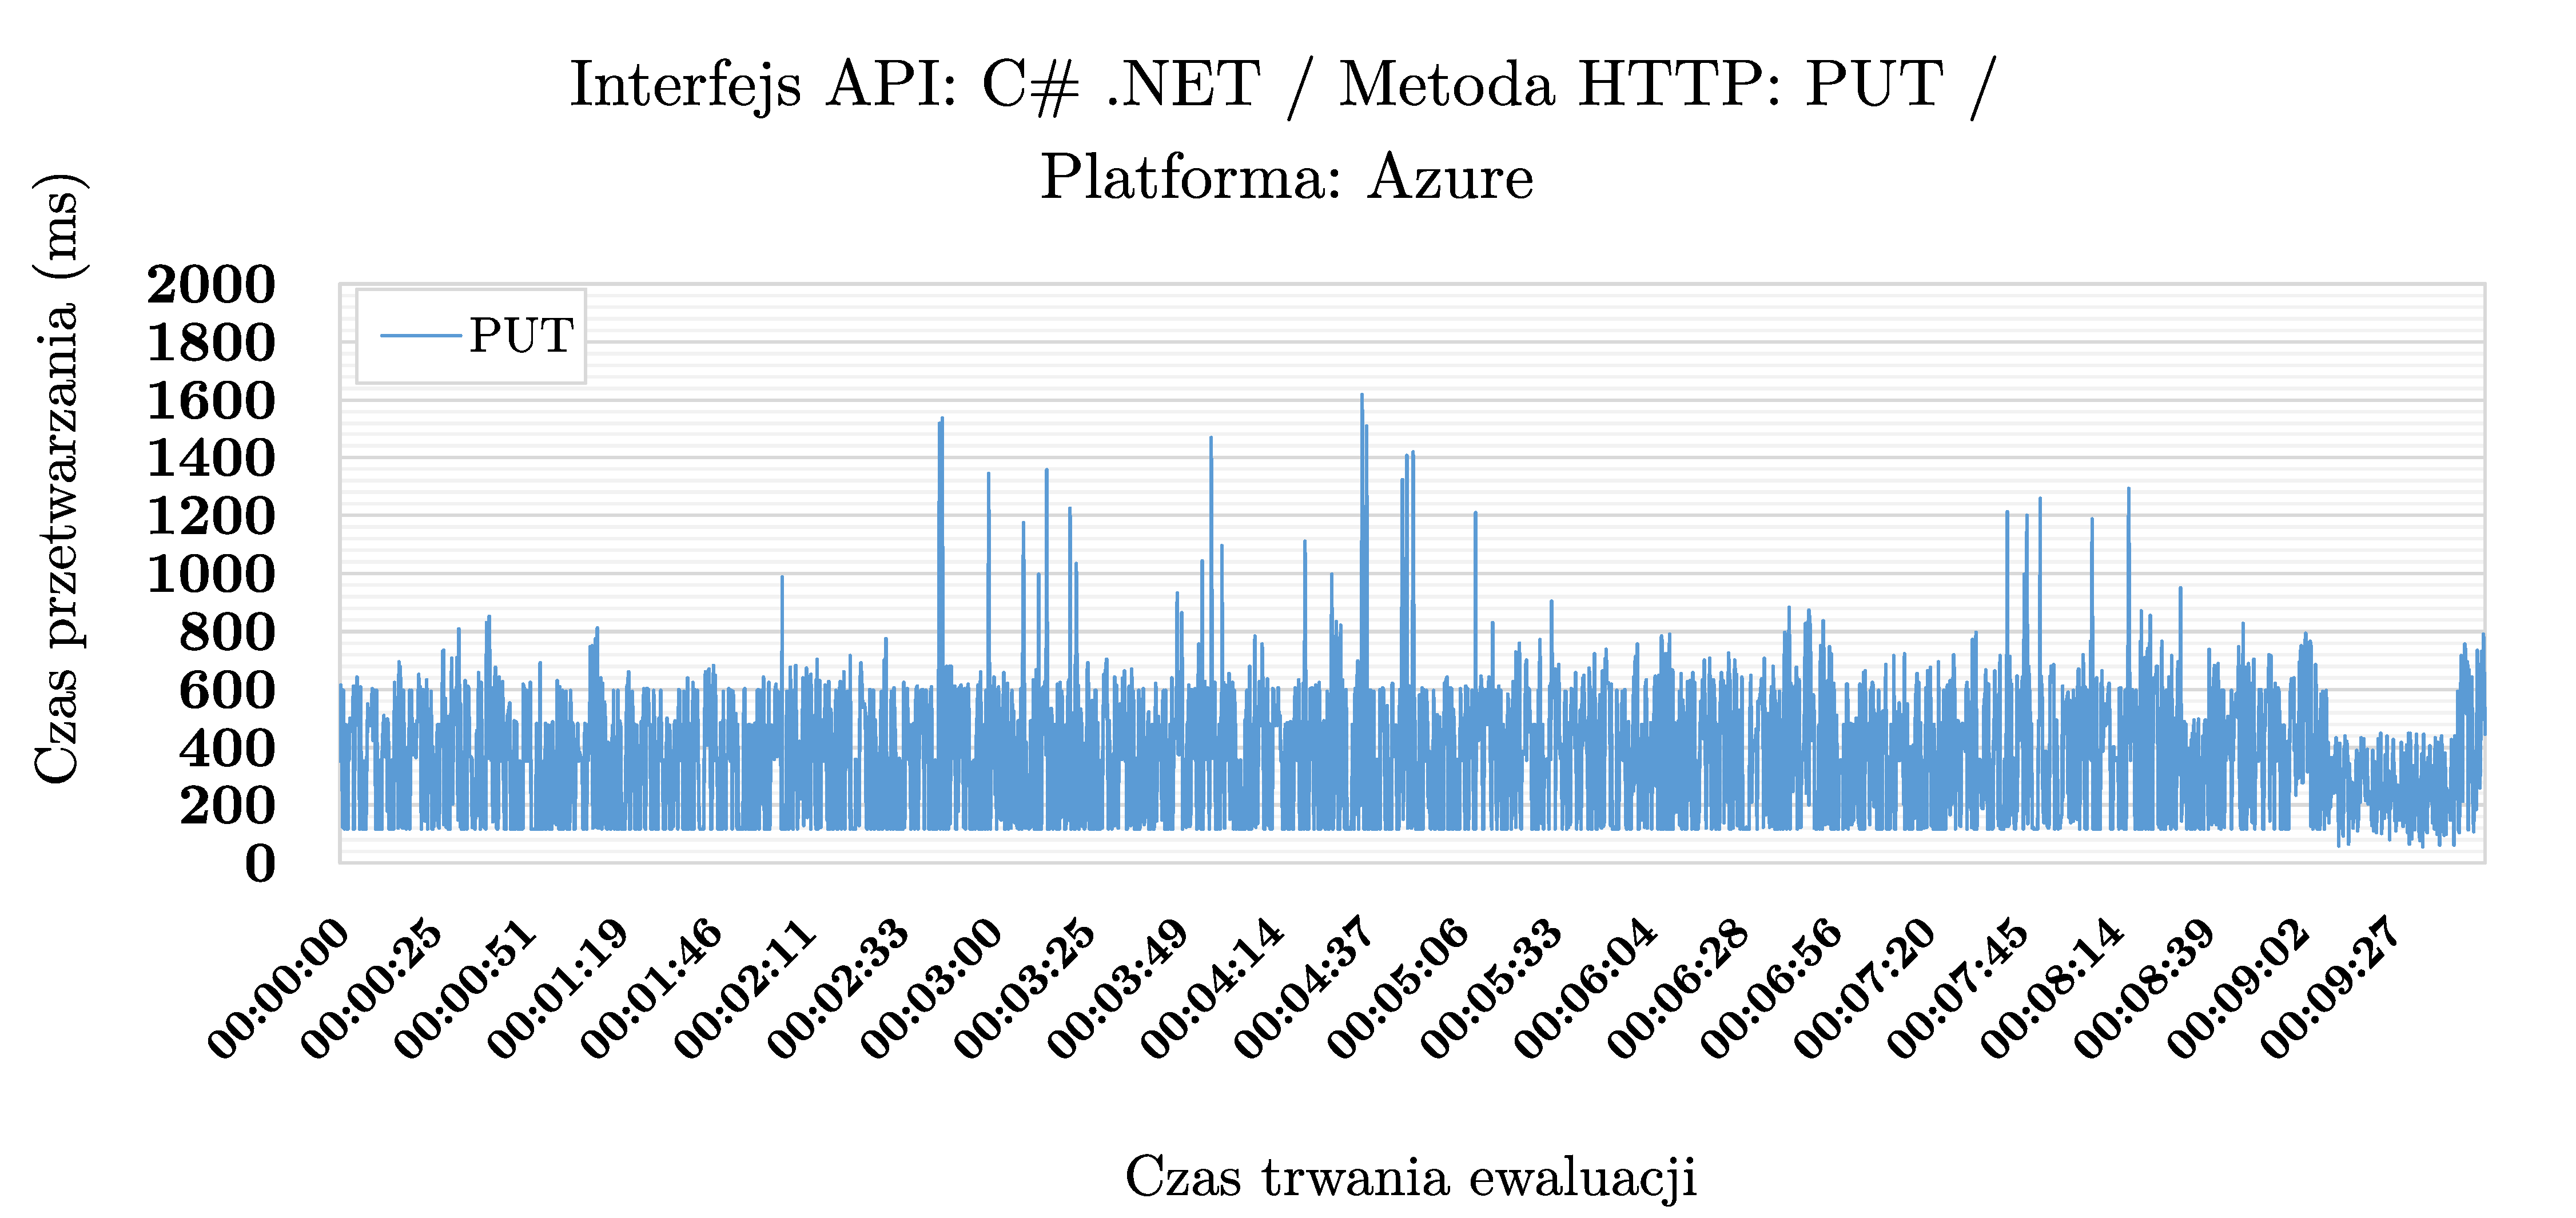
\includegraphics[width=0.49\textwidth]{rys05/dotnet-put-azure.pdf} & 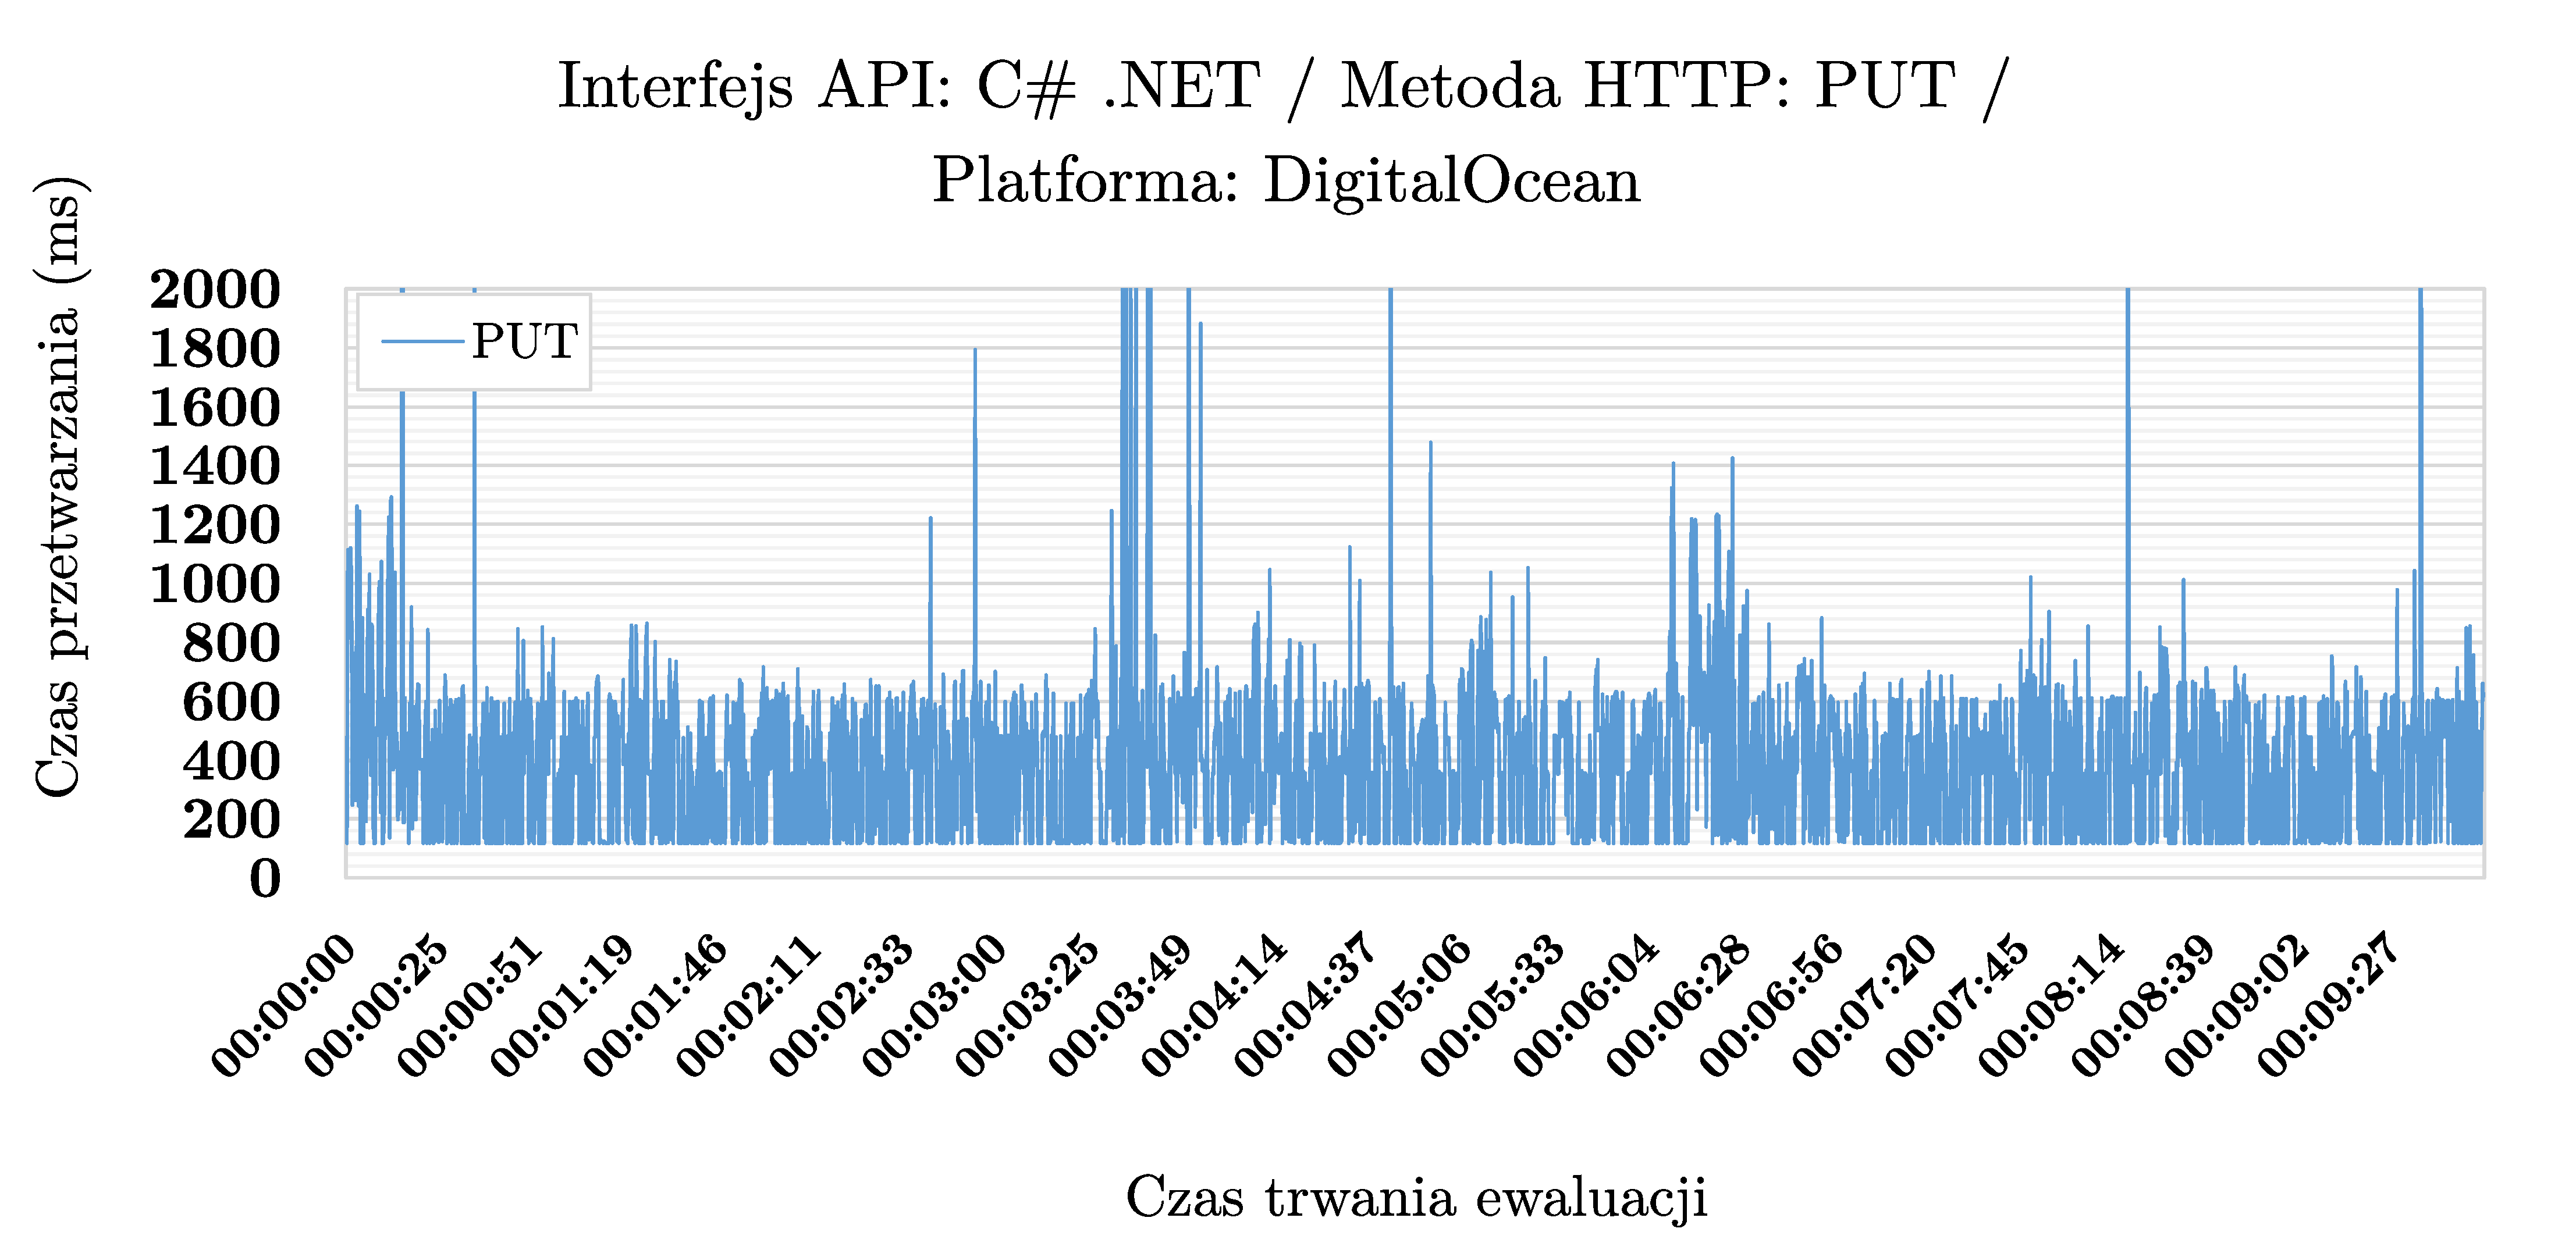
\includegraphics[width=0.49\textwidth]{rys05/dotnet-put-digitalocean.pdf} \\
    g) & h) \\
    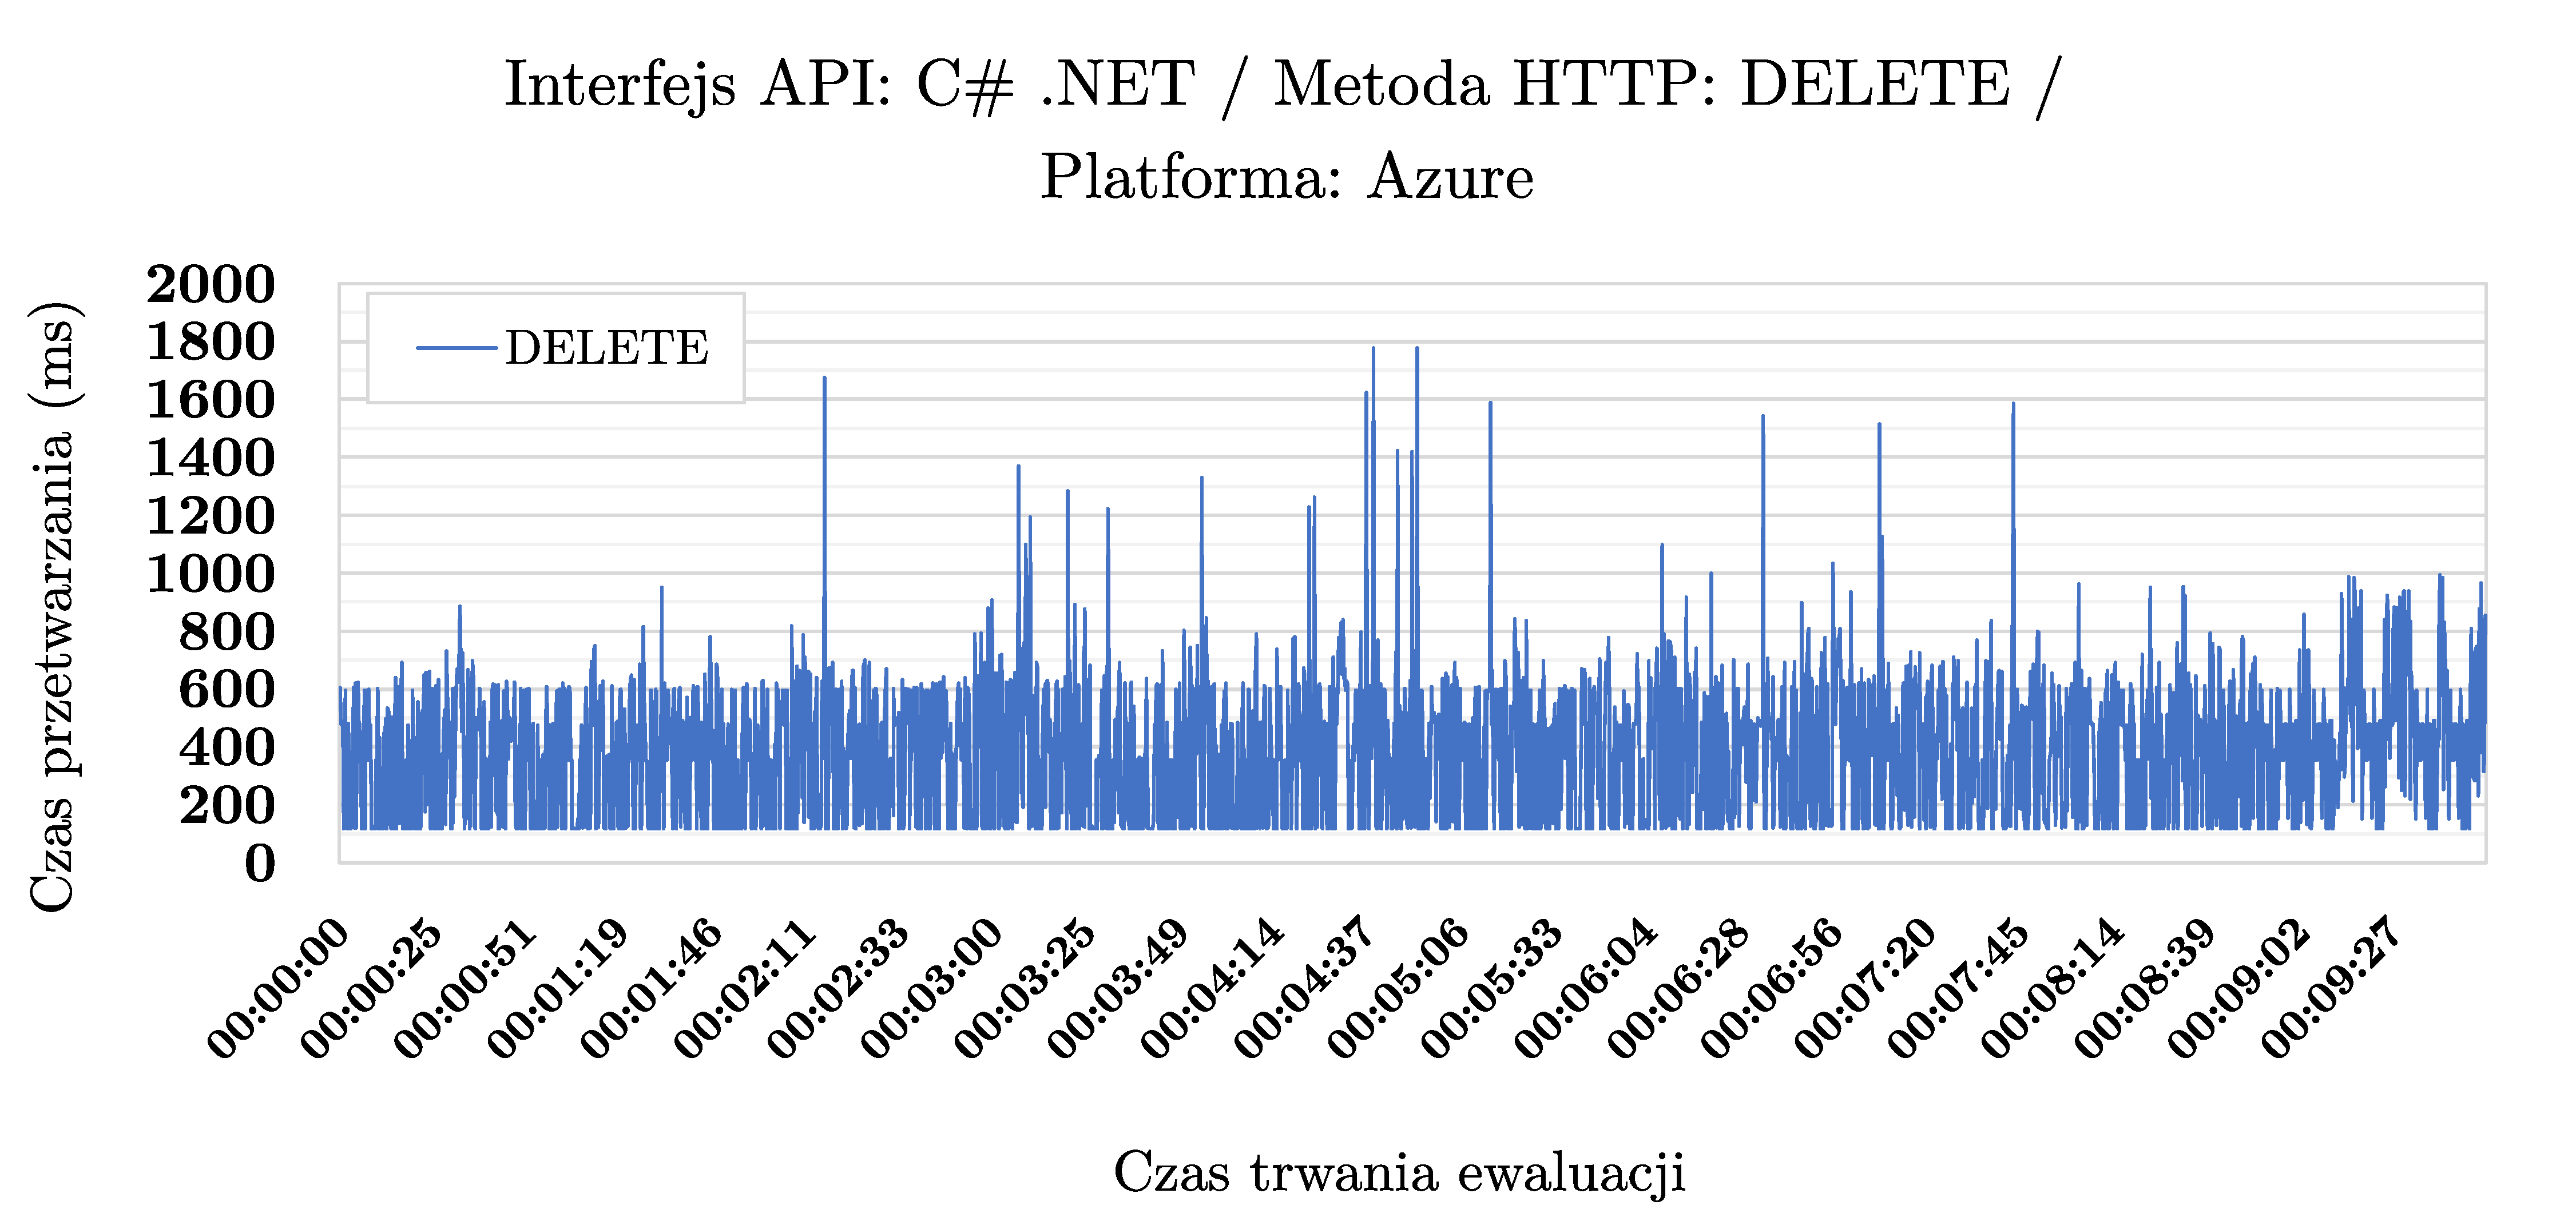
\includegraphics[width=0.49\textwidth]{rys05/dotnet-delete-azure.pdf} & 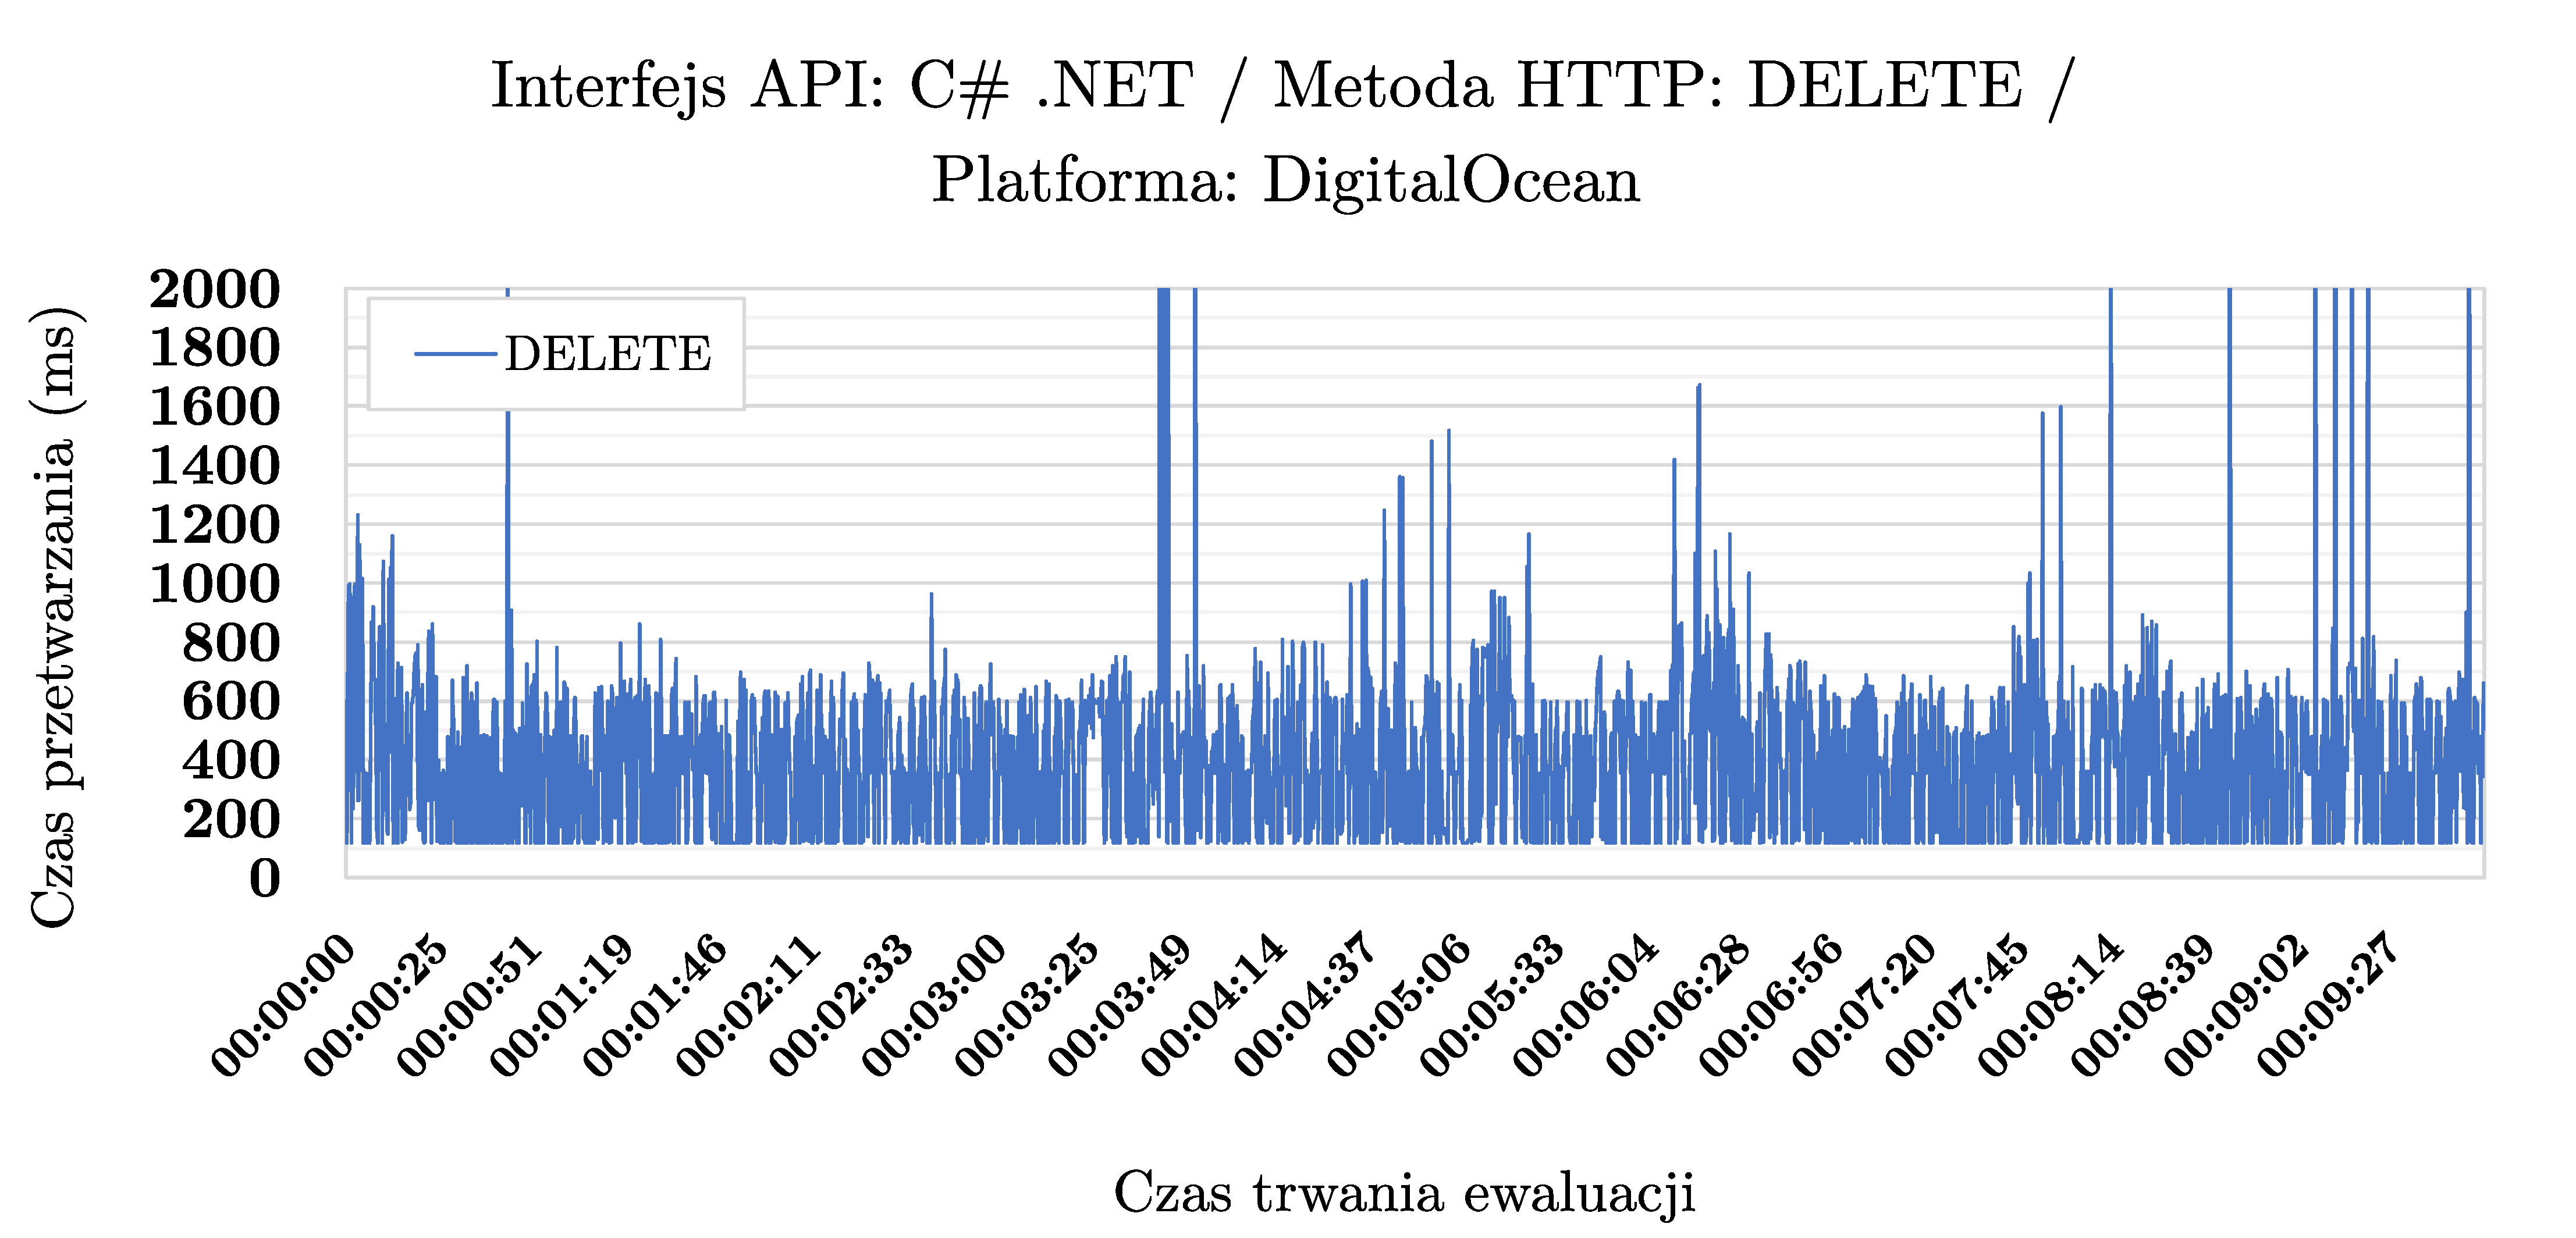
\includegraphics[width=0.49\textwidth]{rys05/dotnet-delete-digitalocean.pdf} \\
	% jezeli obraki sa rownej wysokosci, mozna je wyrownac do gory stosujac vtop jak nizej
	% \vtop{\vskip-2ex\hbox{{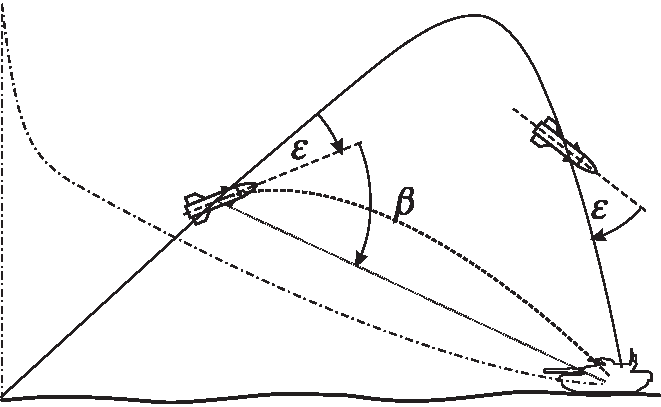
\includegraphics[width=0.475\textwidth]{rys05/beta1}}}} &
	% \vtop{\vskip-2ex\hbox{{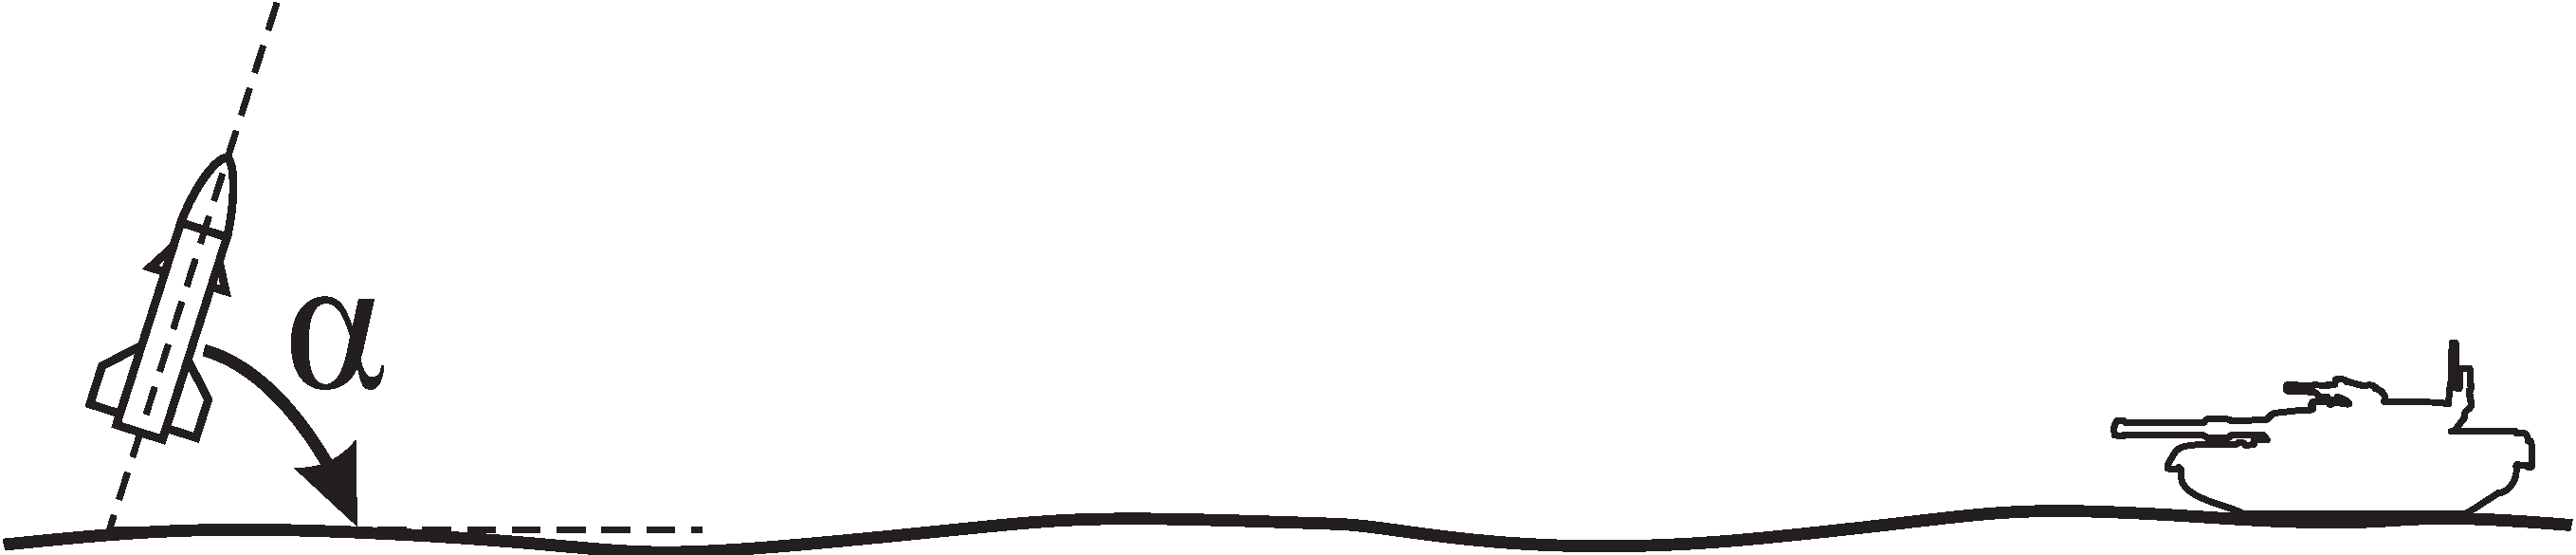
\includegraphics[width=0.475\textwidth]{rys05/alfa1}}}}  \caption{Wyznaczanie trajektorii lotu rakiety: 
	\end{tabular}
  \caption{Wydajność działania mierzona czasem wewnętrznego przetwarzania operacji CRUD dla platform Azure oraz DigitalOcean -- Interfejs API C\# .NET}
  \label{fig:dotnet-azure-vs-digitalocean}
\end{figure}

Wskazać należy nieznaczą, jednakże występującą przewagę rozwiązania opartego o usługę platform-as-a-service. Jak możemy zauważyć, przewaga ta, występuje niezależnie od typu generowanego żądania klienta. Ponadto, w przypadku rozwiązania generycznego zaobserwowano pojawienie się większej liczby zapytań klienckich, których czasy odpowiedzi nie mieściły się w przedziale definiującym 97\% wszystkich próbek (tj. od 200 ms do 580 ms) dla rozwiązania dedykowanego. Szczególnie trend ten, widoczny jest dla żądań metody HTTP typu PUT. Wartym odnotowania jest fakt niewystępowania jakiegokolwiek wyniku w przedziale od 0 do 119 ms. Wyniki takie, były bez trudu osiągane w środowisku lokalnym dla małej liczby współbieżnie pracujących generatorów. Zjawisko to, jest specyficzne względem względem technologii C\# .NET i nie uwidacznia się w przypadku interfejsów uruchamianych w NodeJS.

\begin{figure}[H]
  \centering
	\begin{tabular}{@{}ll@{}}
    a) & b) \\
    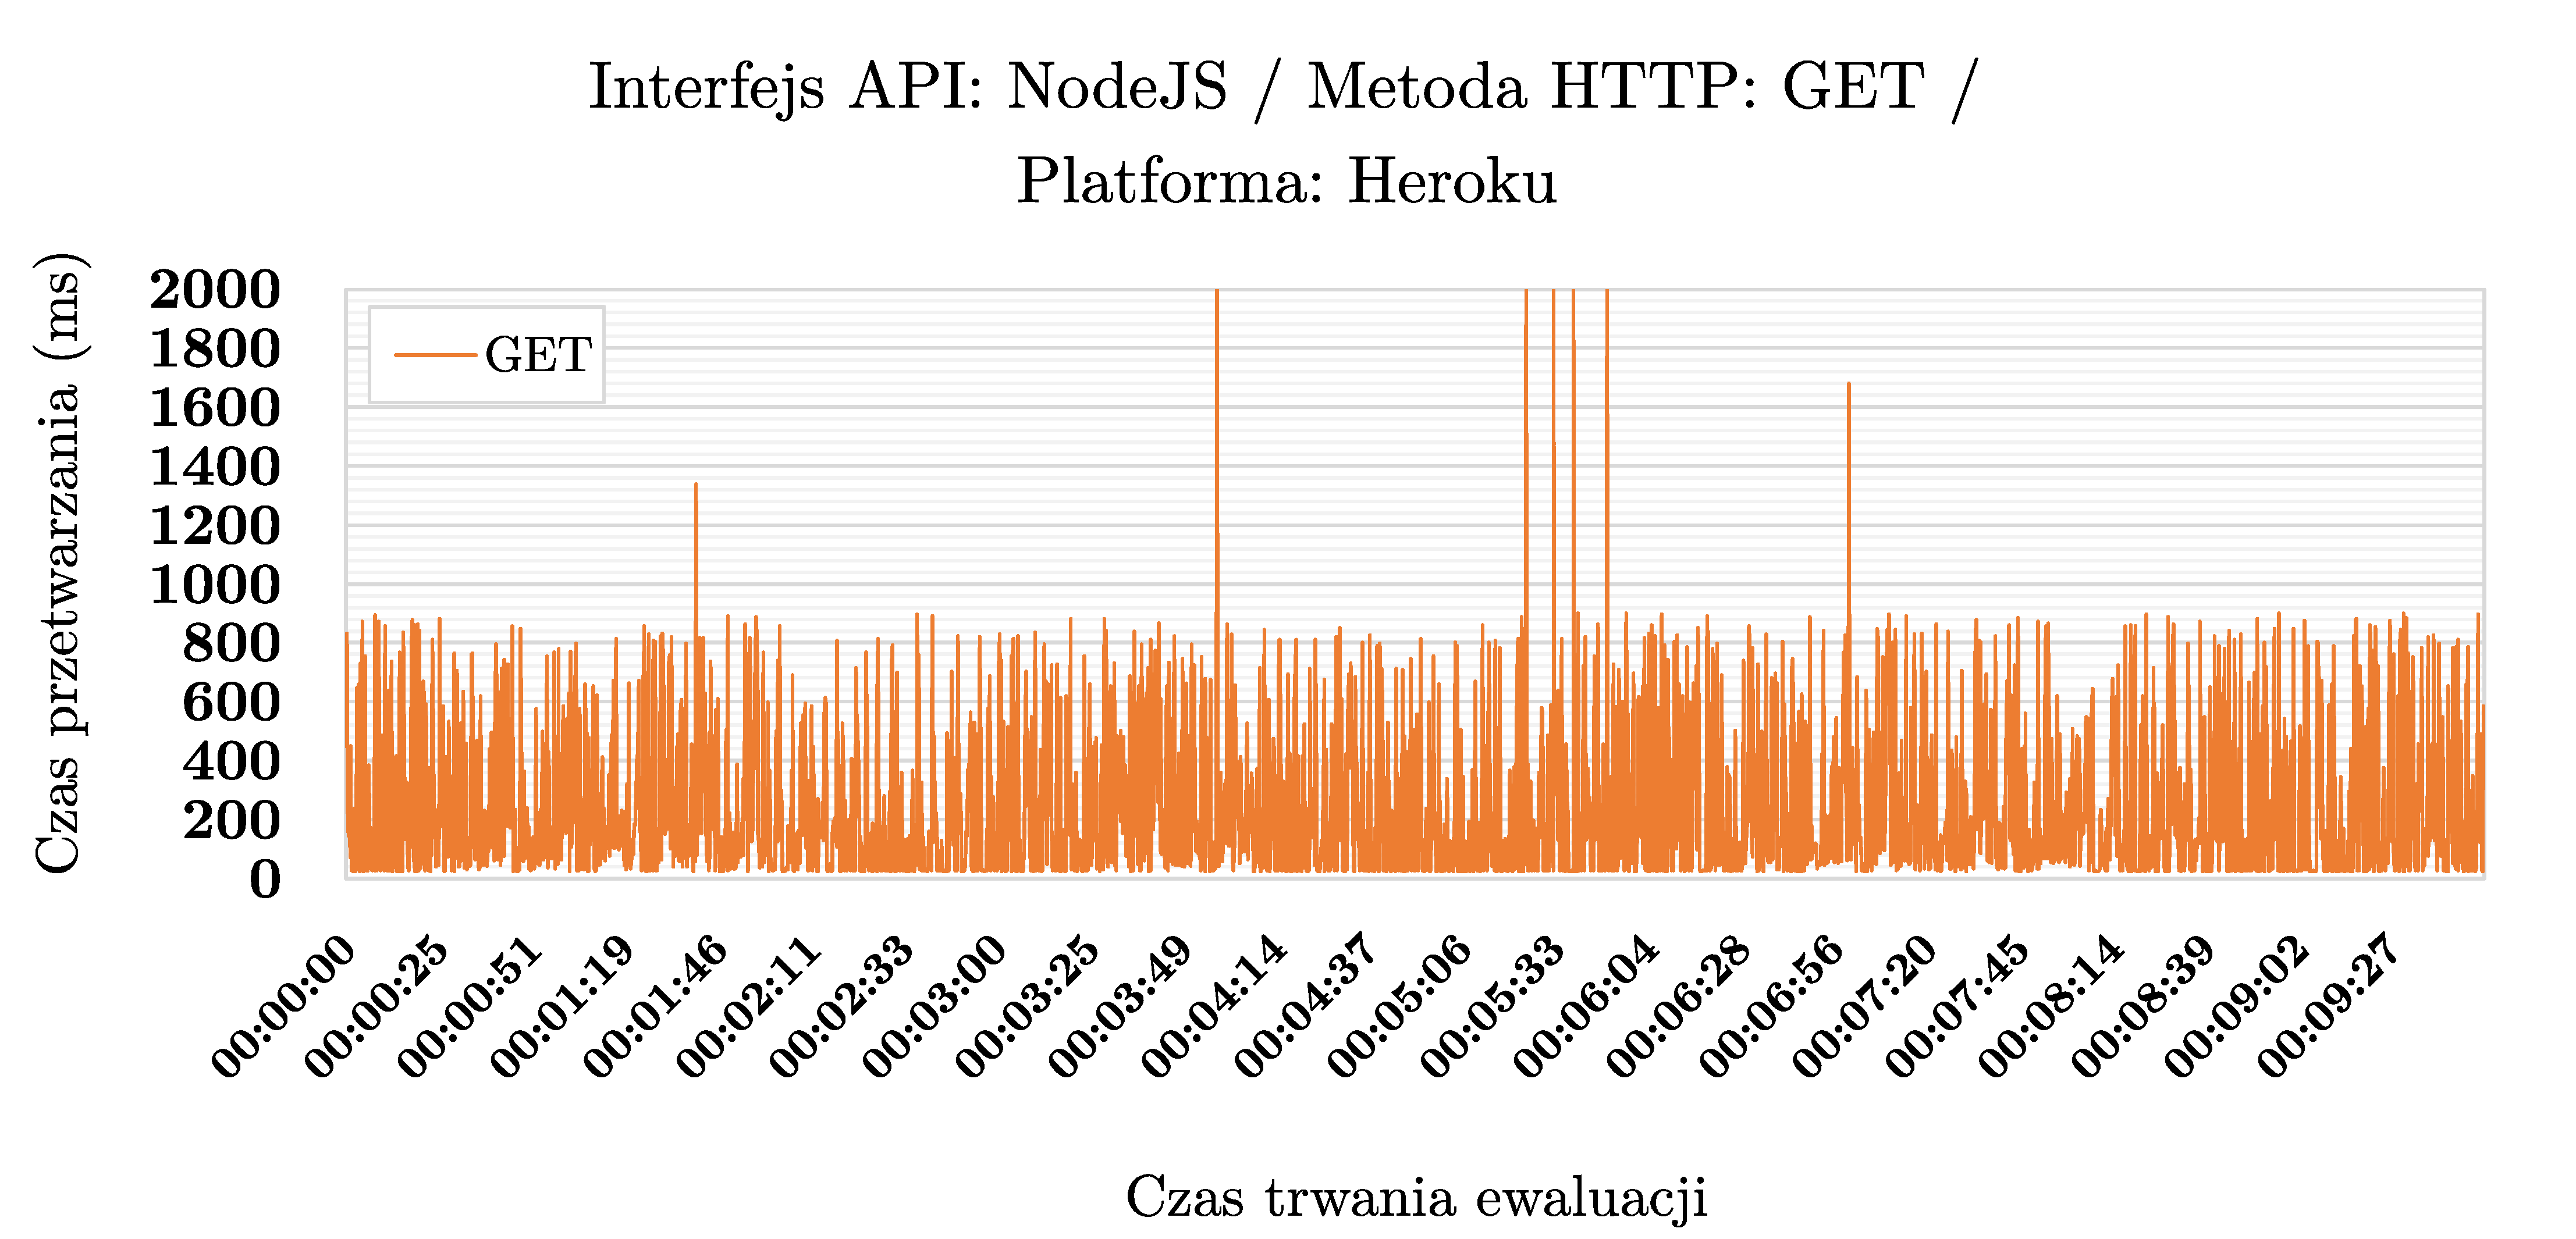
\includegraphics[width=0.49\textwidth]{rys05/nodejs-get-heroku.pdf} & 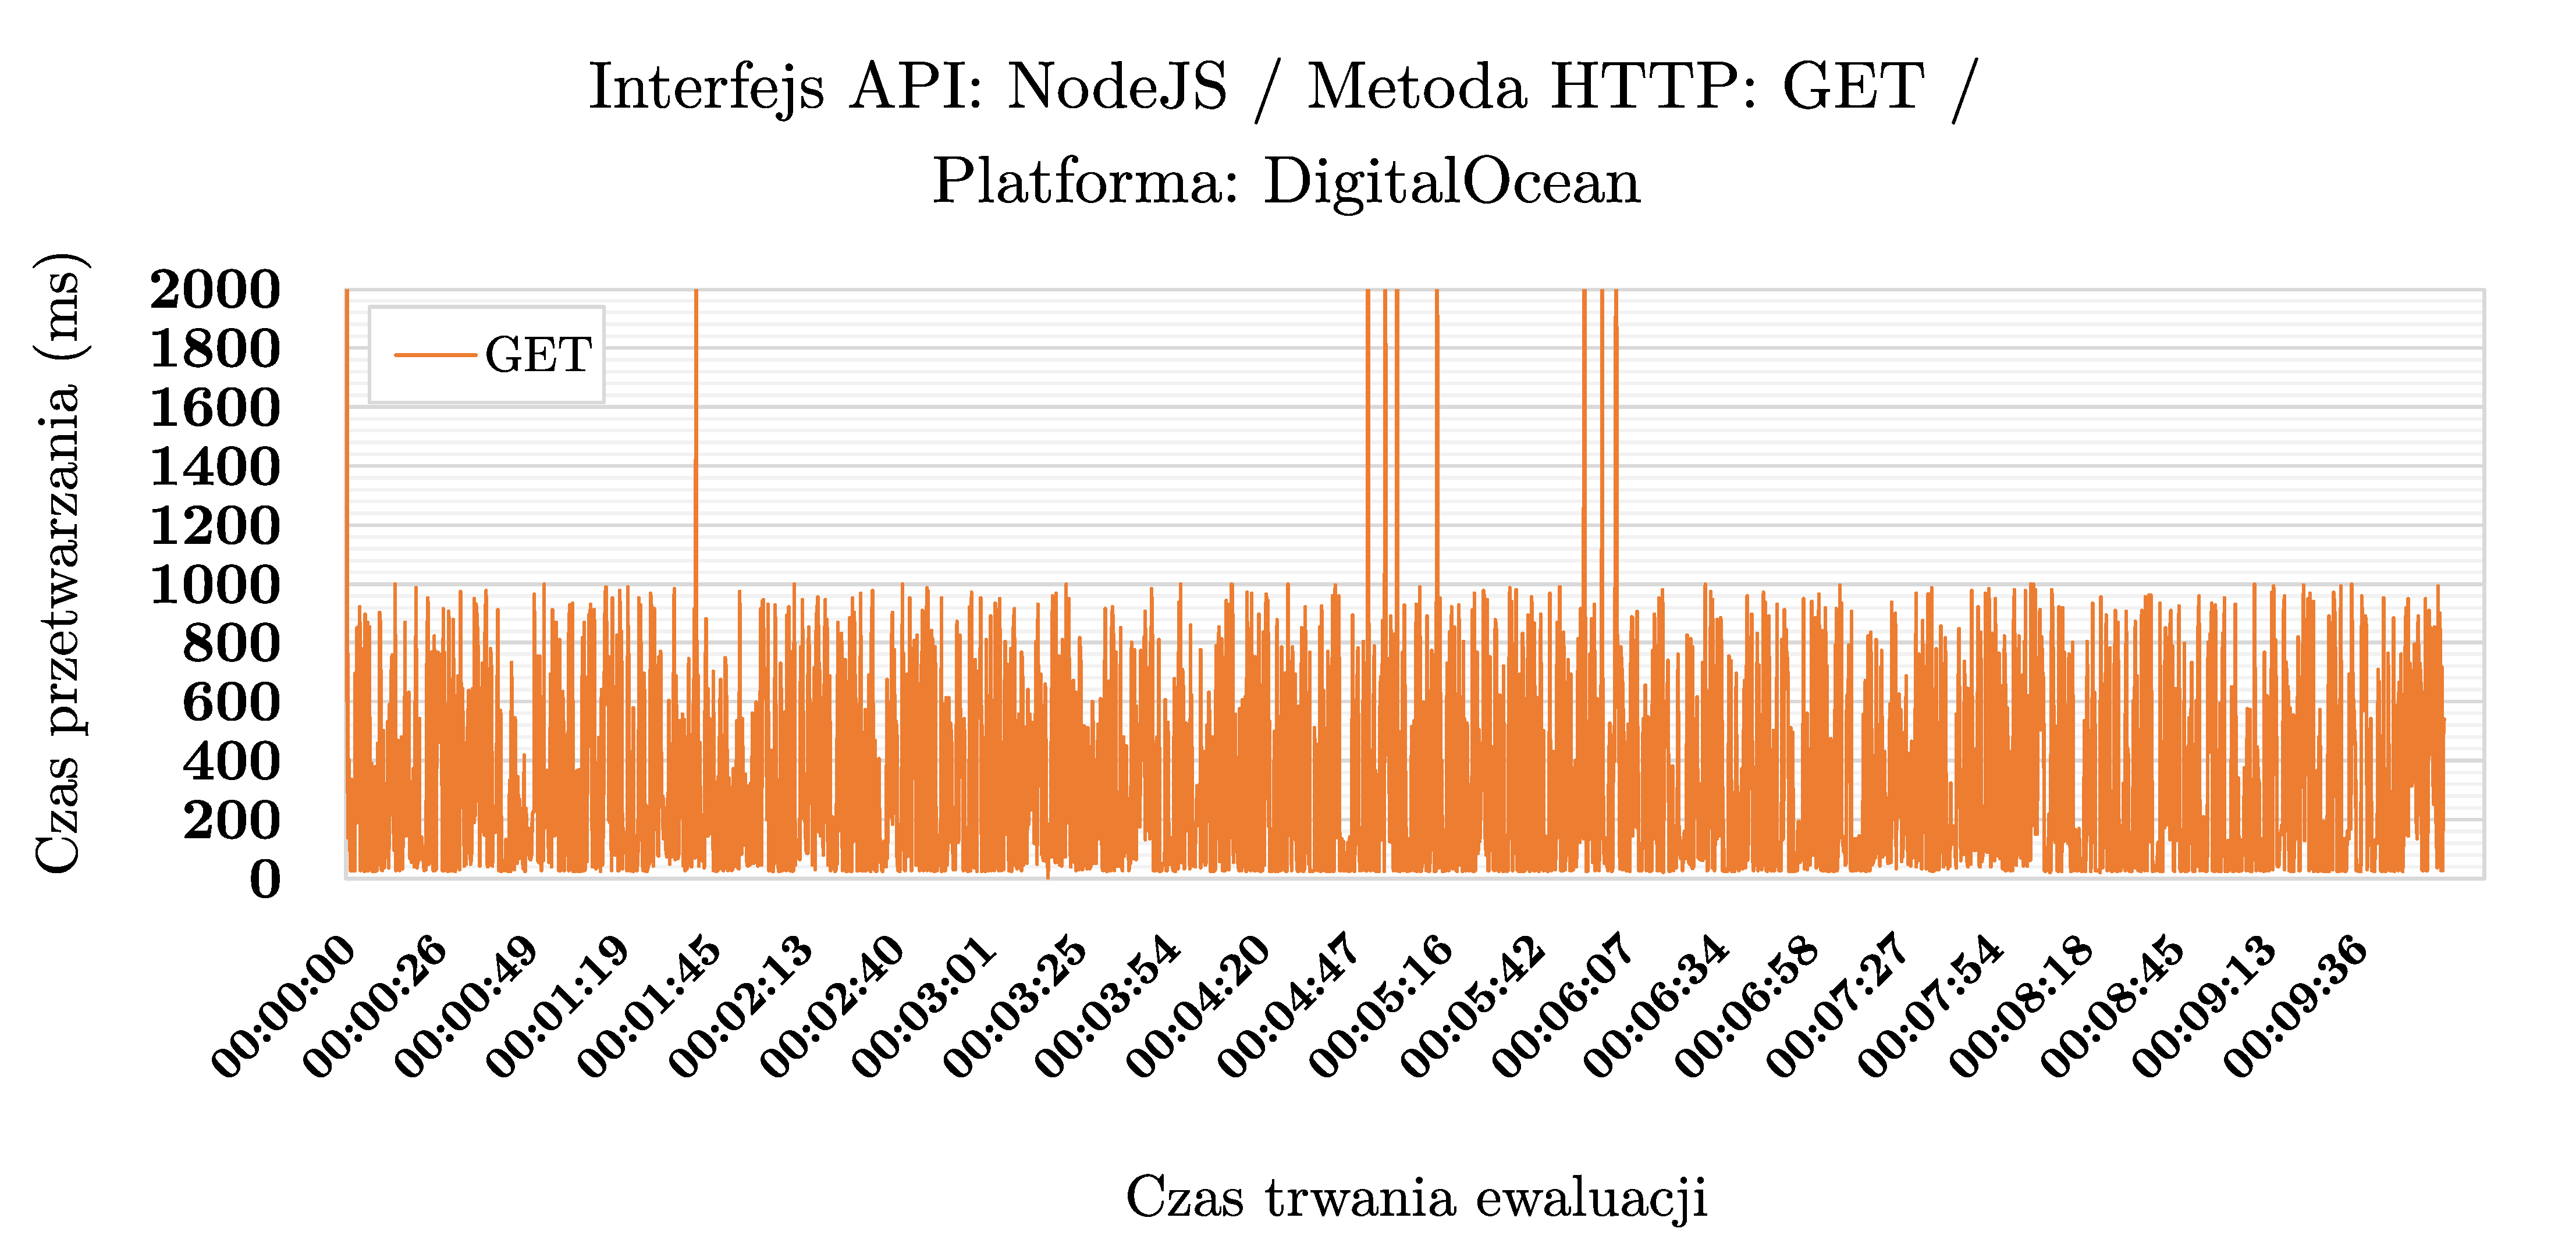
\includegraphics[width=0.49\textwidth]{rys05/nodejs-get-digitalocean.pdf} \\
    c) & d) \\
    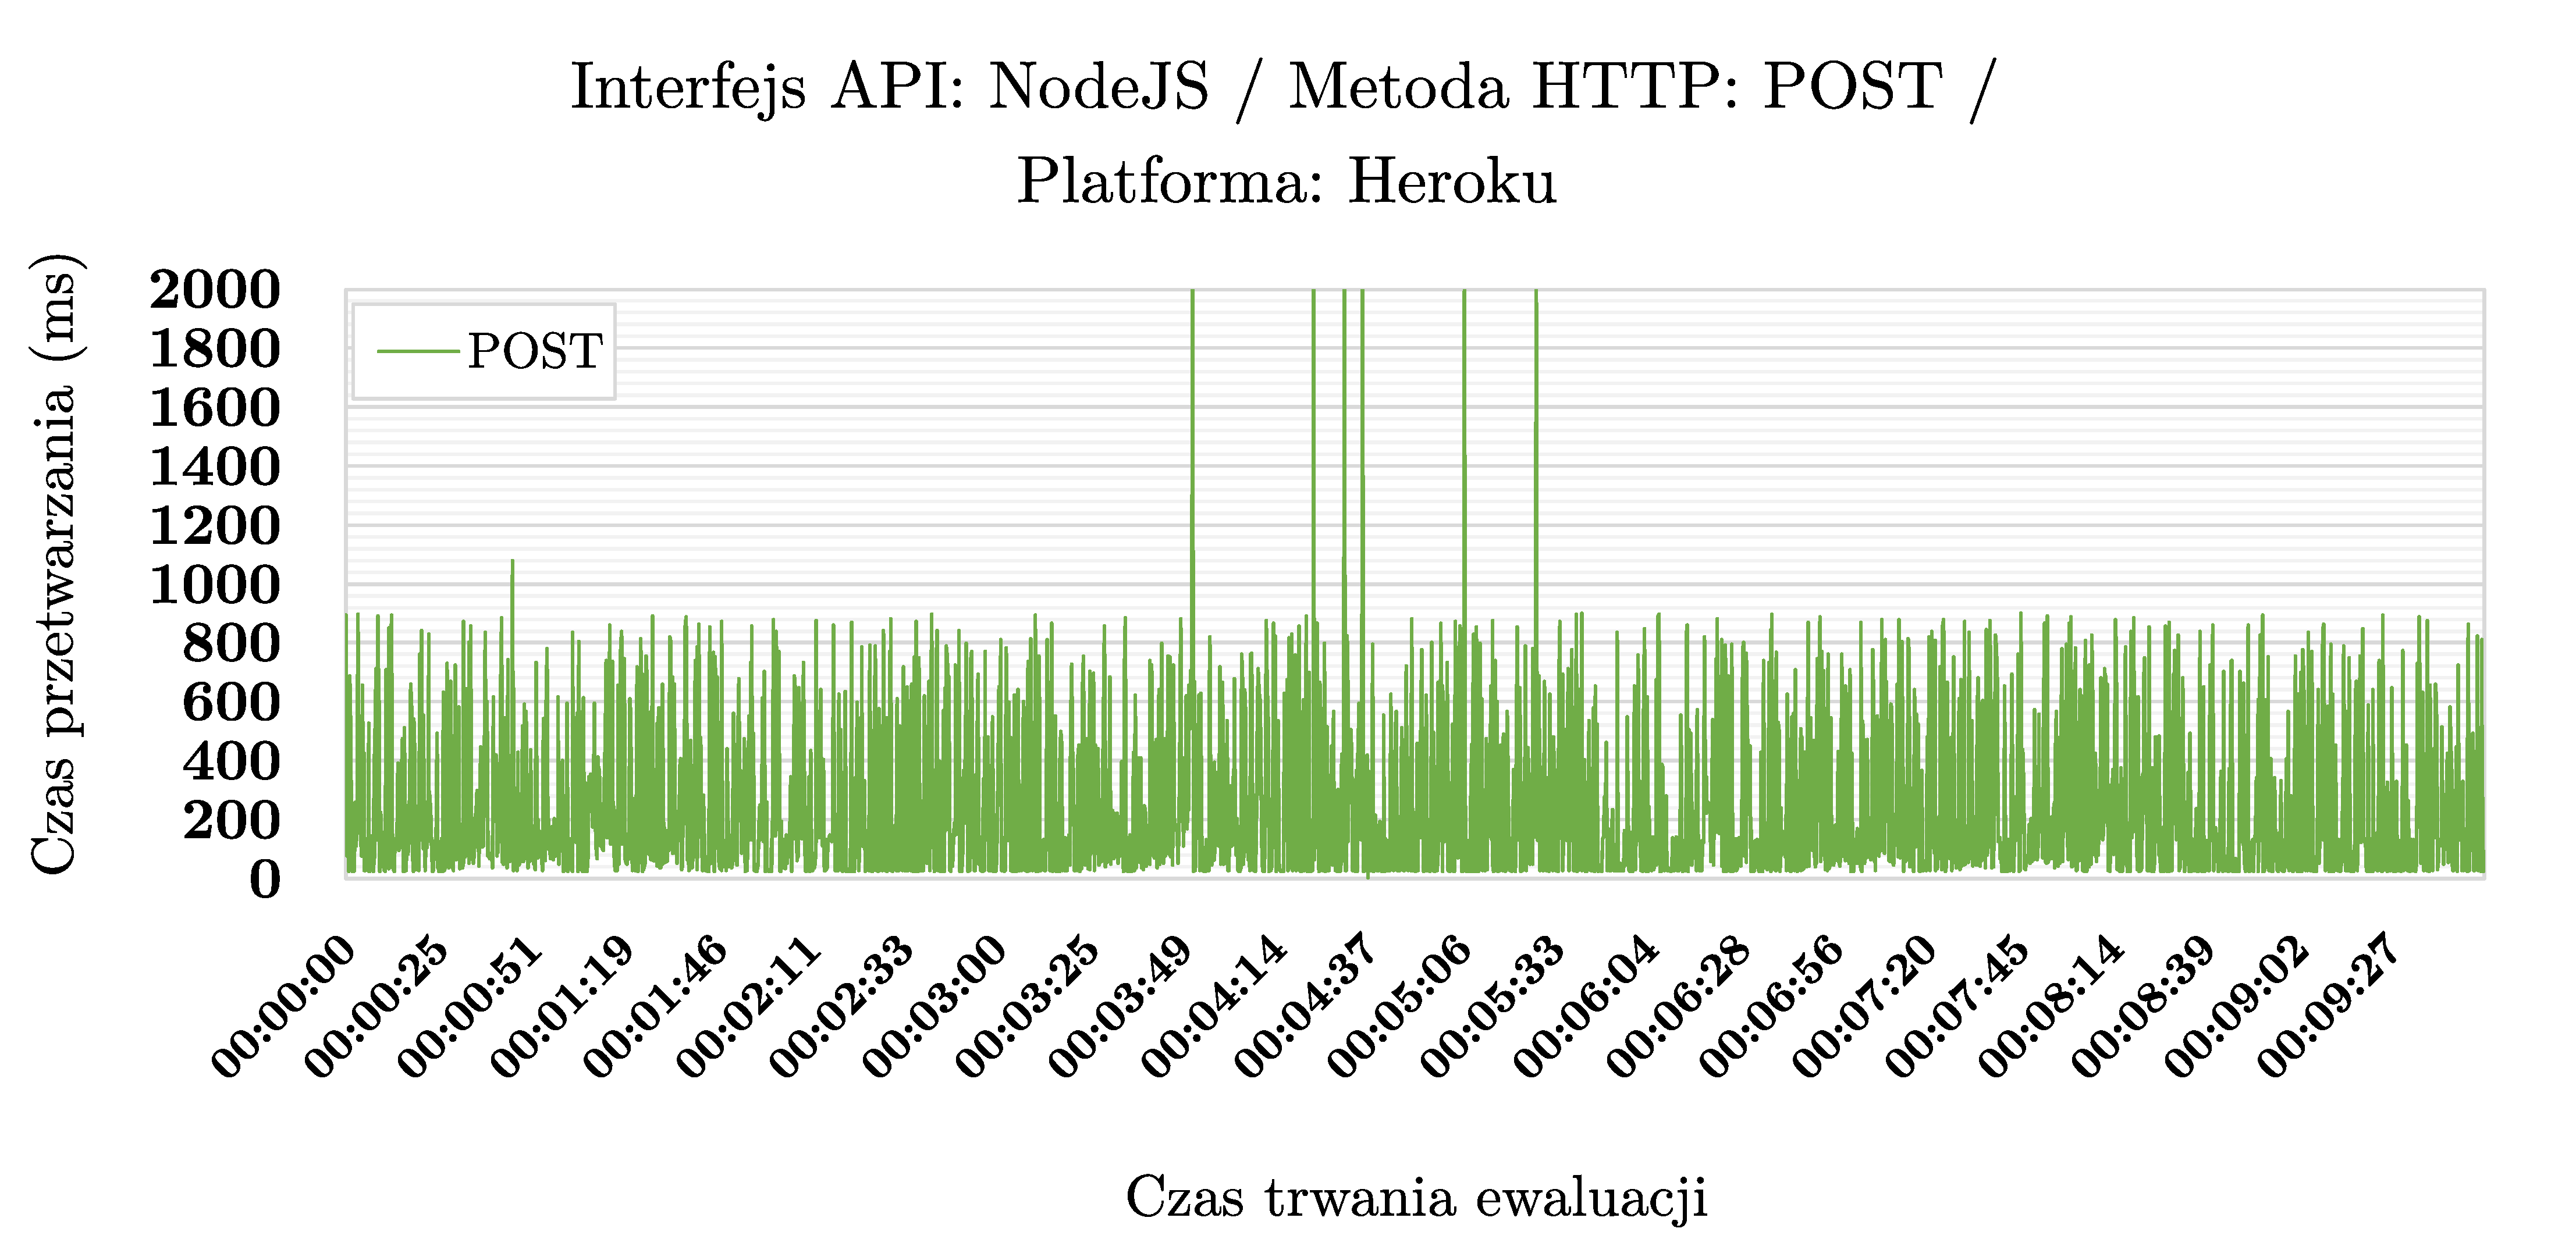
\includegraphics[width=0.49\textwidth]{rys05/nodejs-post-heroku.pdf} & 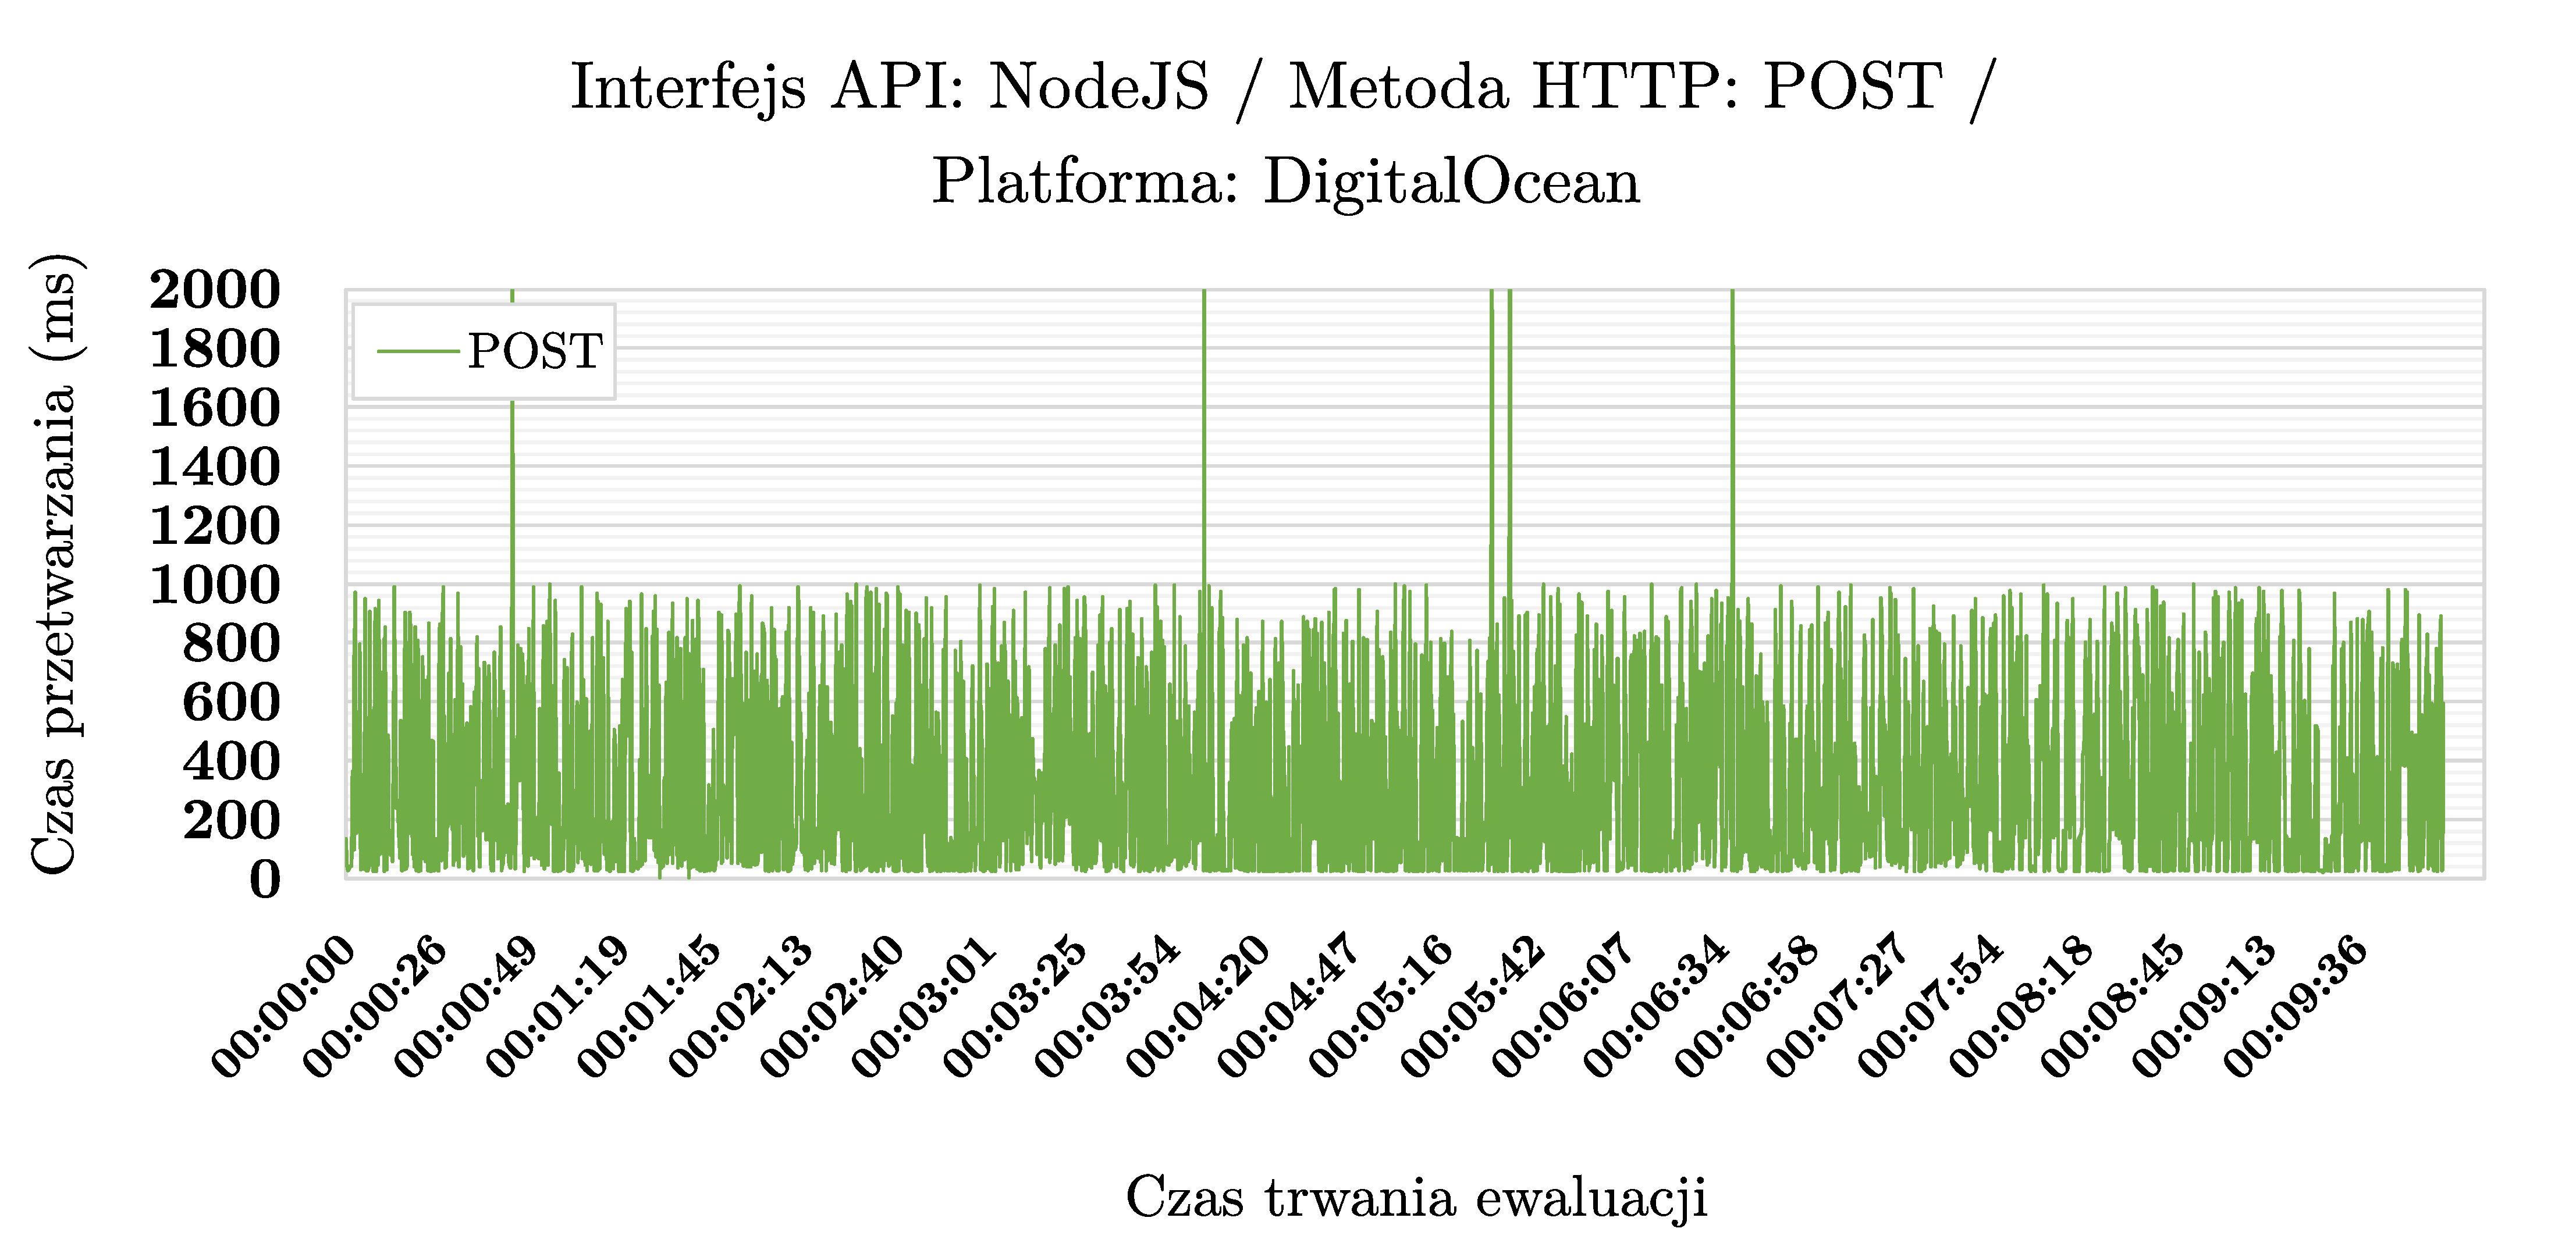
\includegraphics[width=0.49\textwidth]{rys05/nodejs-post-digitalocean.pdf} \\
    e) & f) \\
    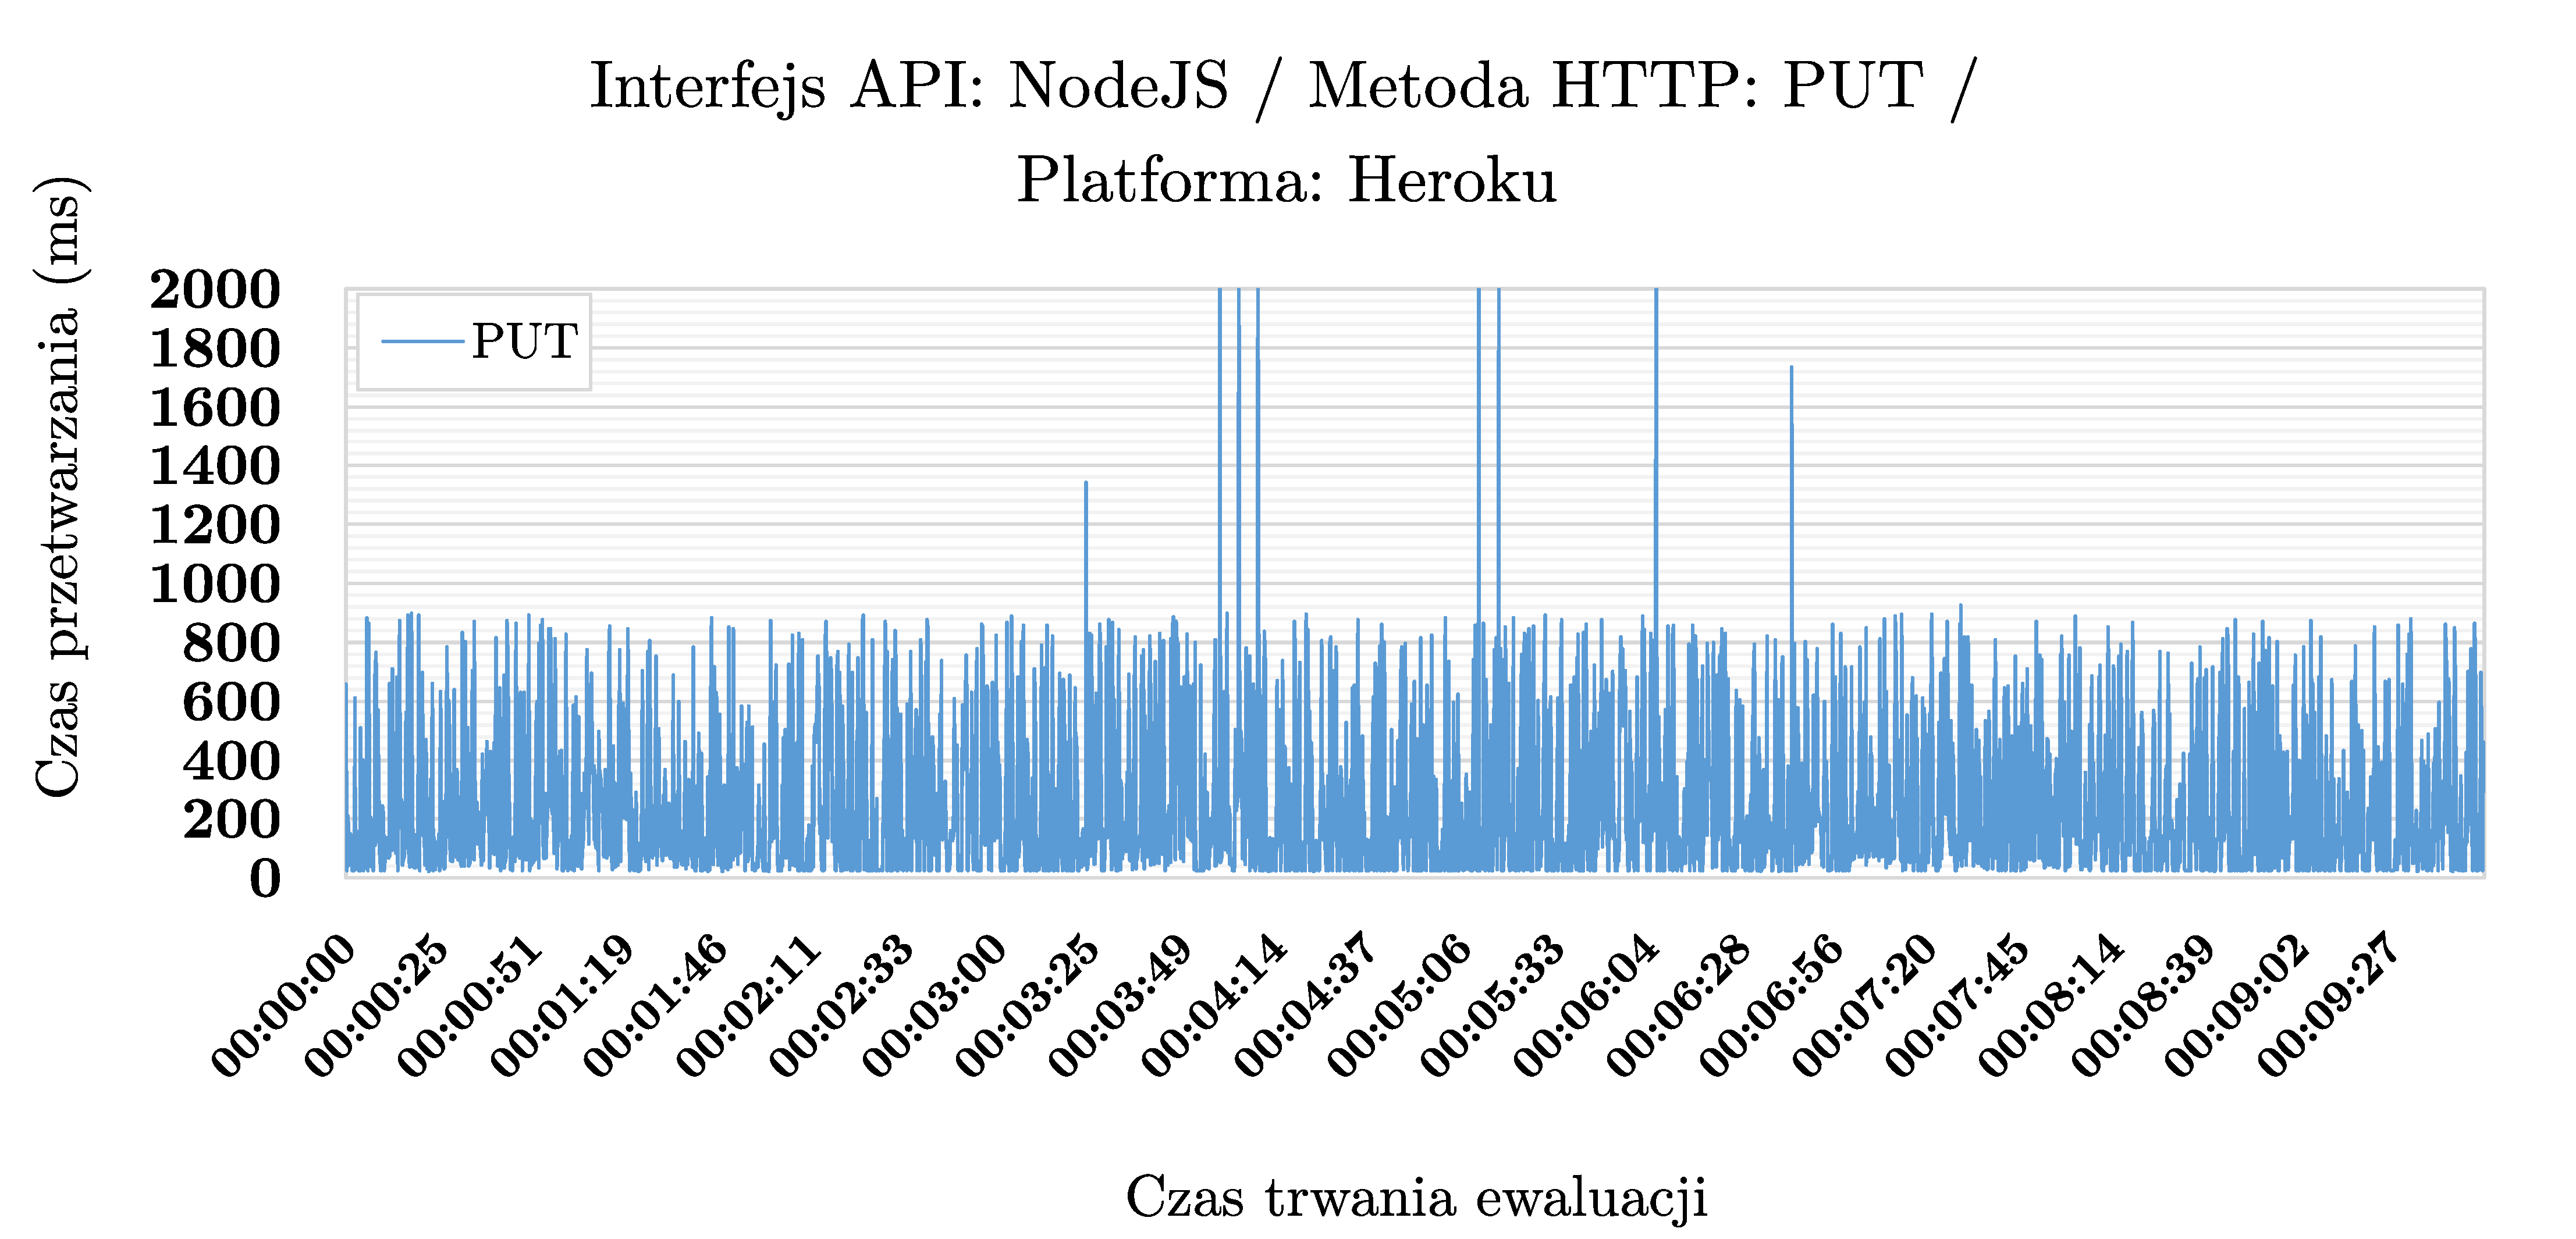
\includegraphics[width=0.49\textwidth]{rys05/nodejs-put-heroku.pdf} & 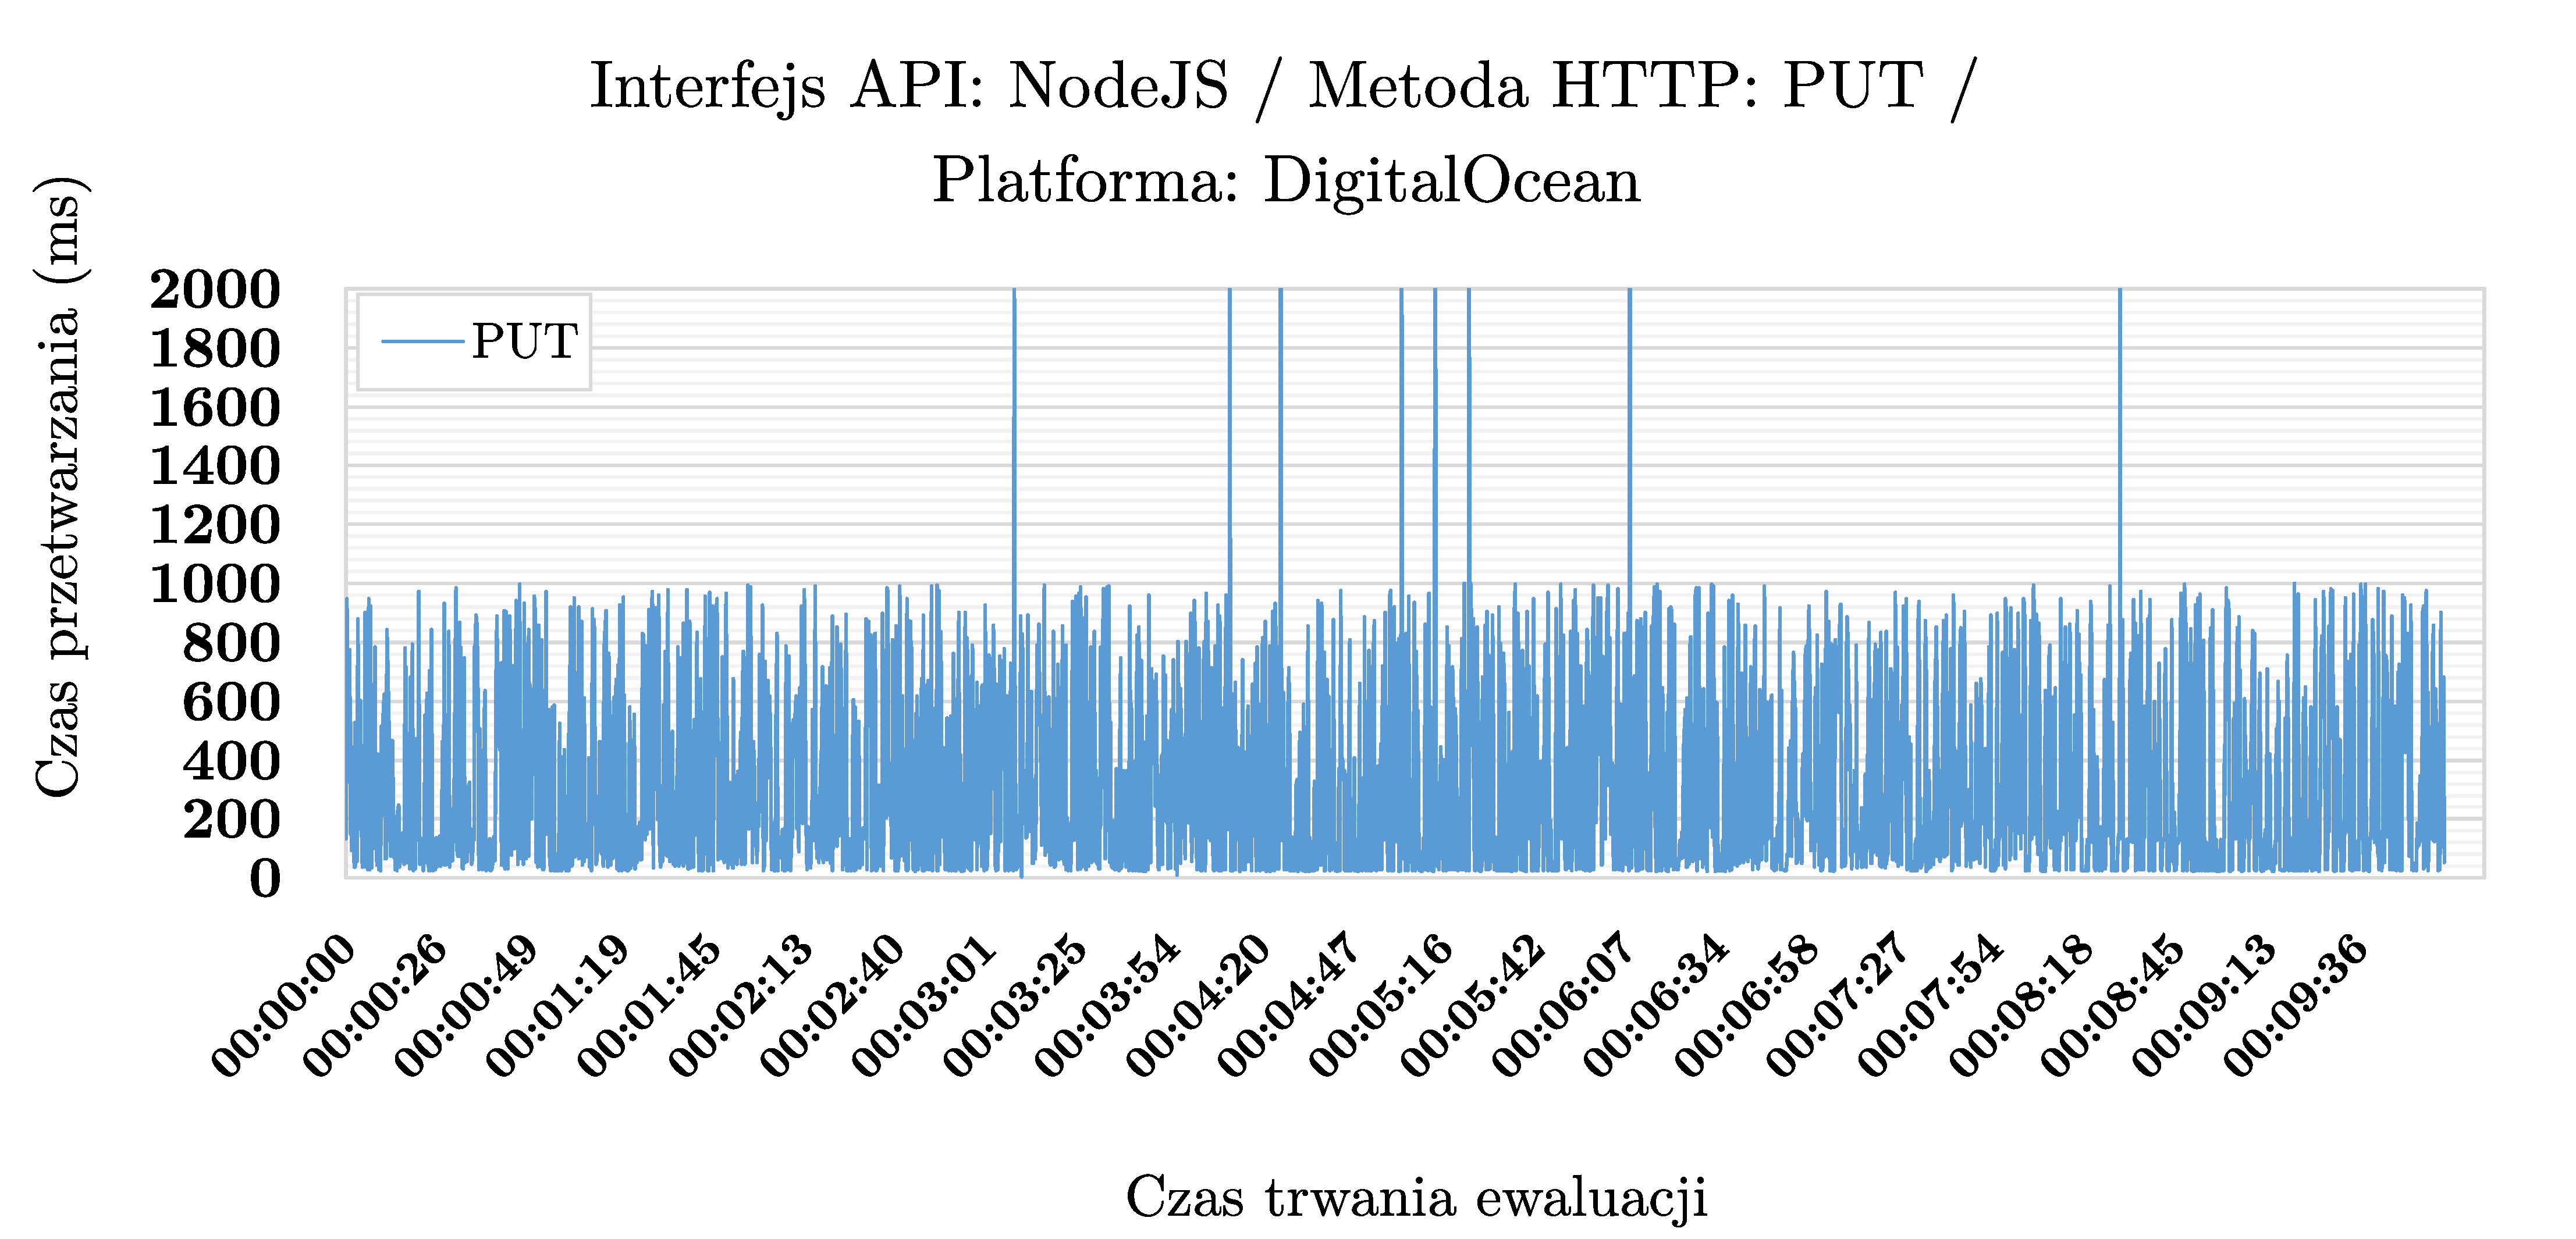
\includegraphics[width=0.49\textwidth]{rys05/nodejs-put-digitalocean.pdf} \\
    g) & h) \\
    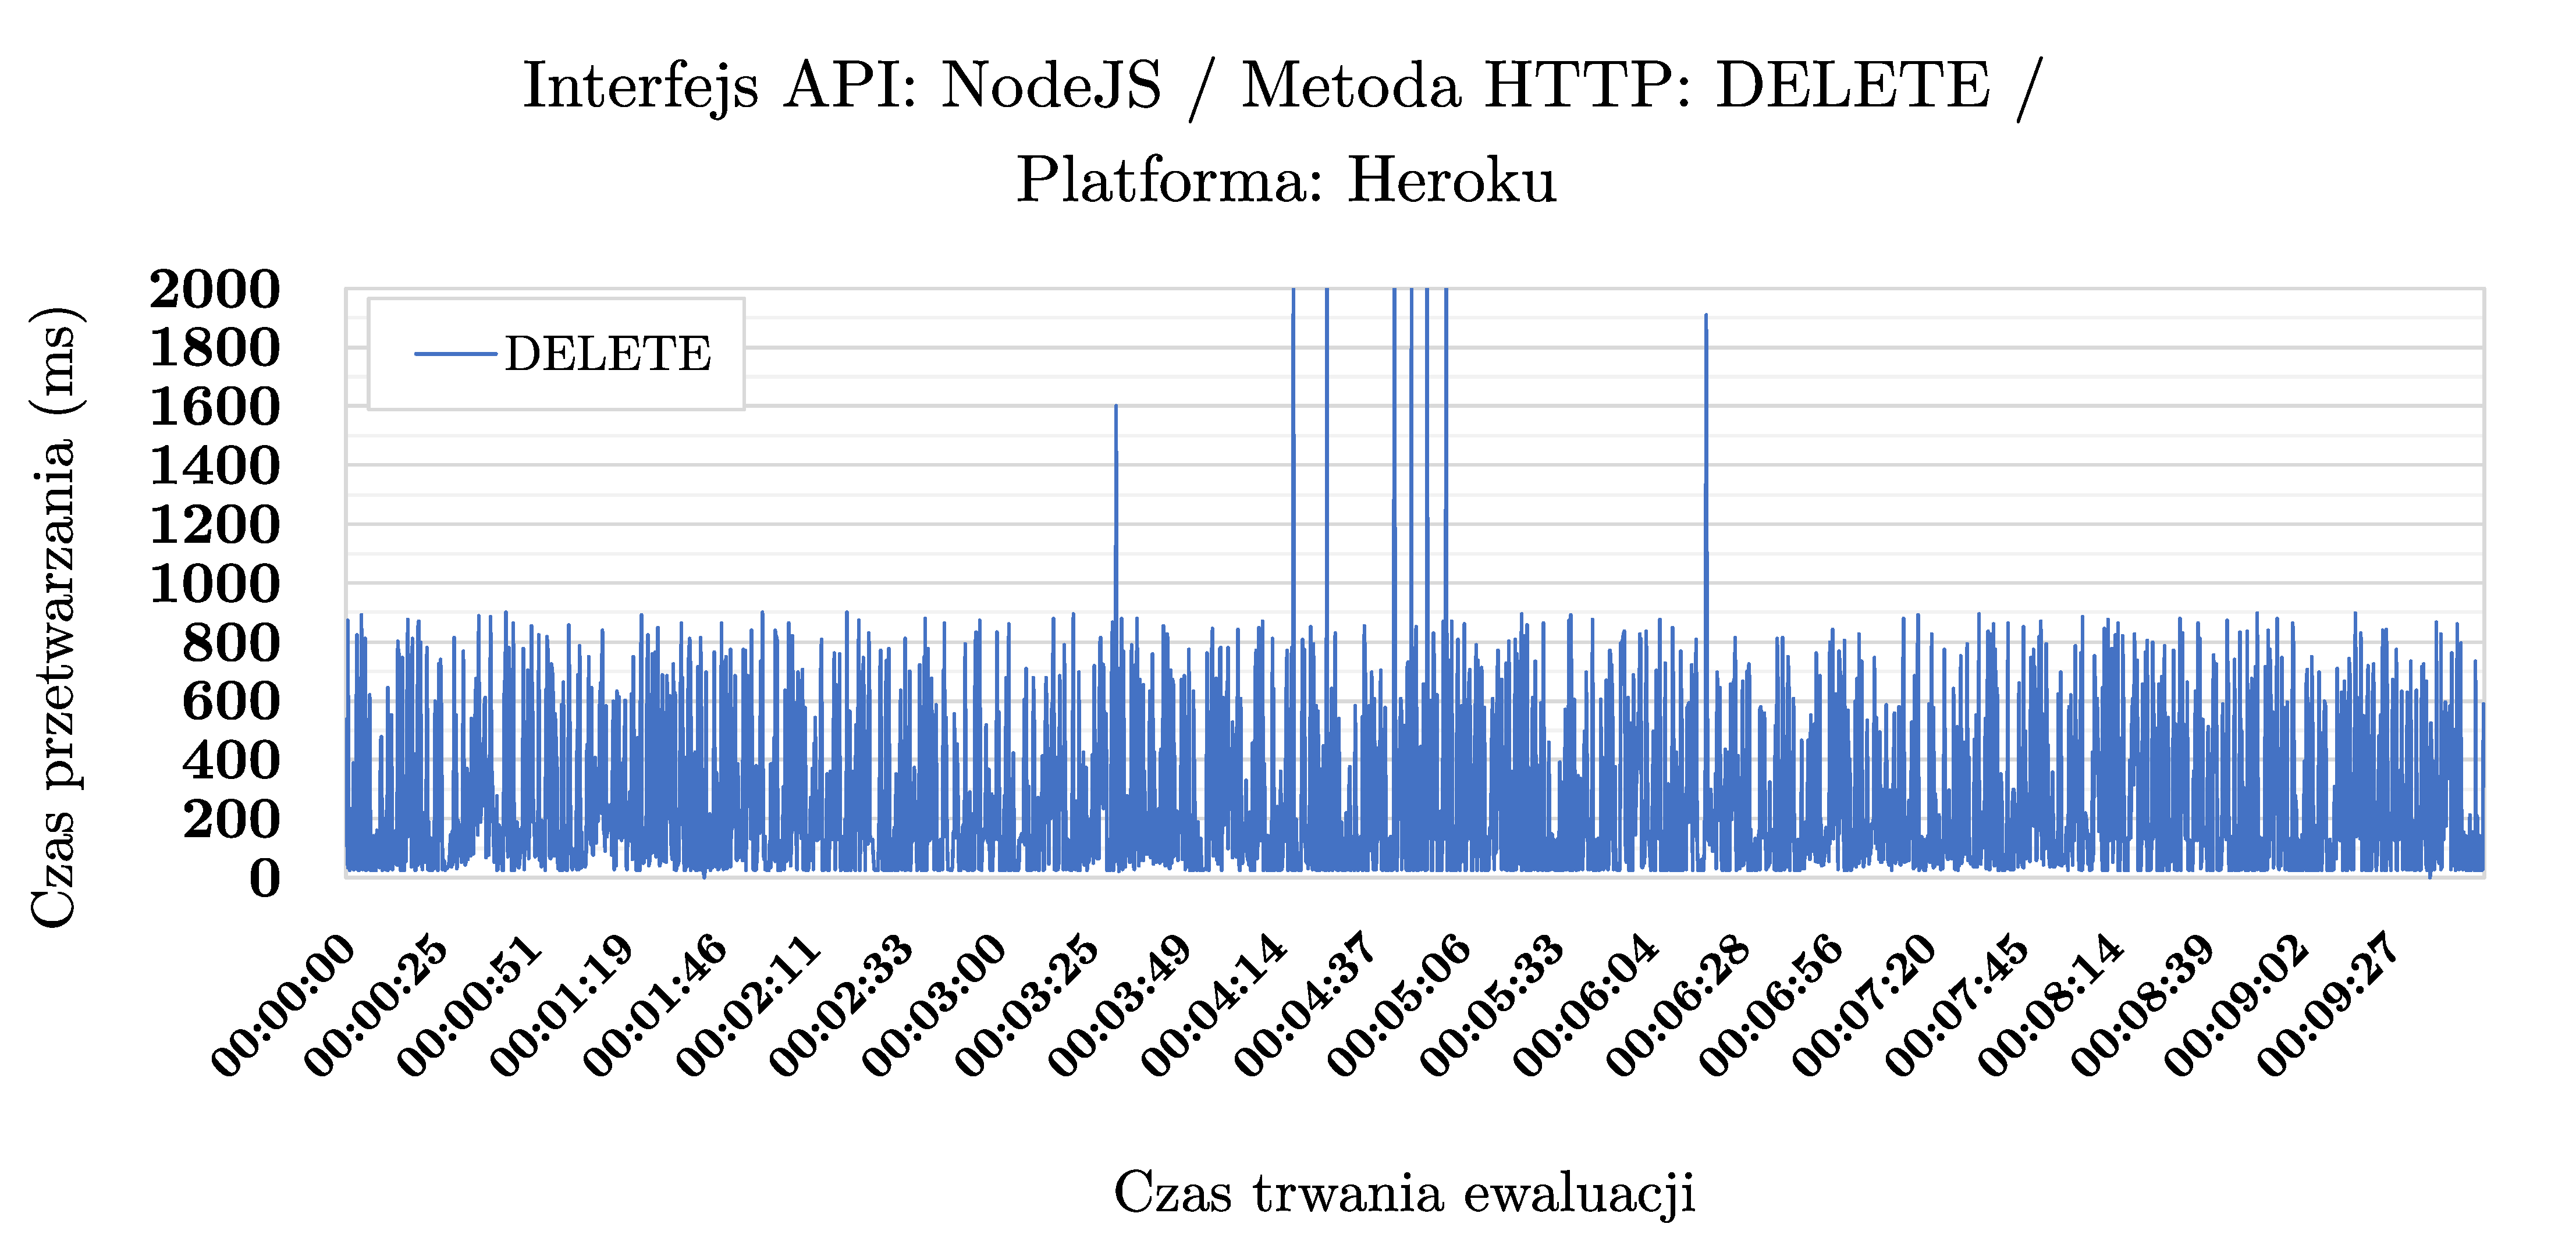
\includegraphics[width=0.49\textwidth]{rys05/nodejs-delete-heroku.pdf} & 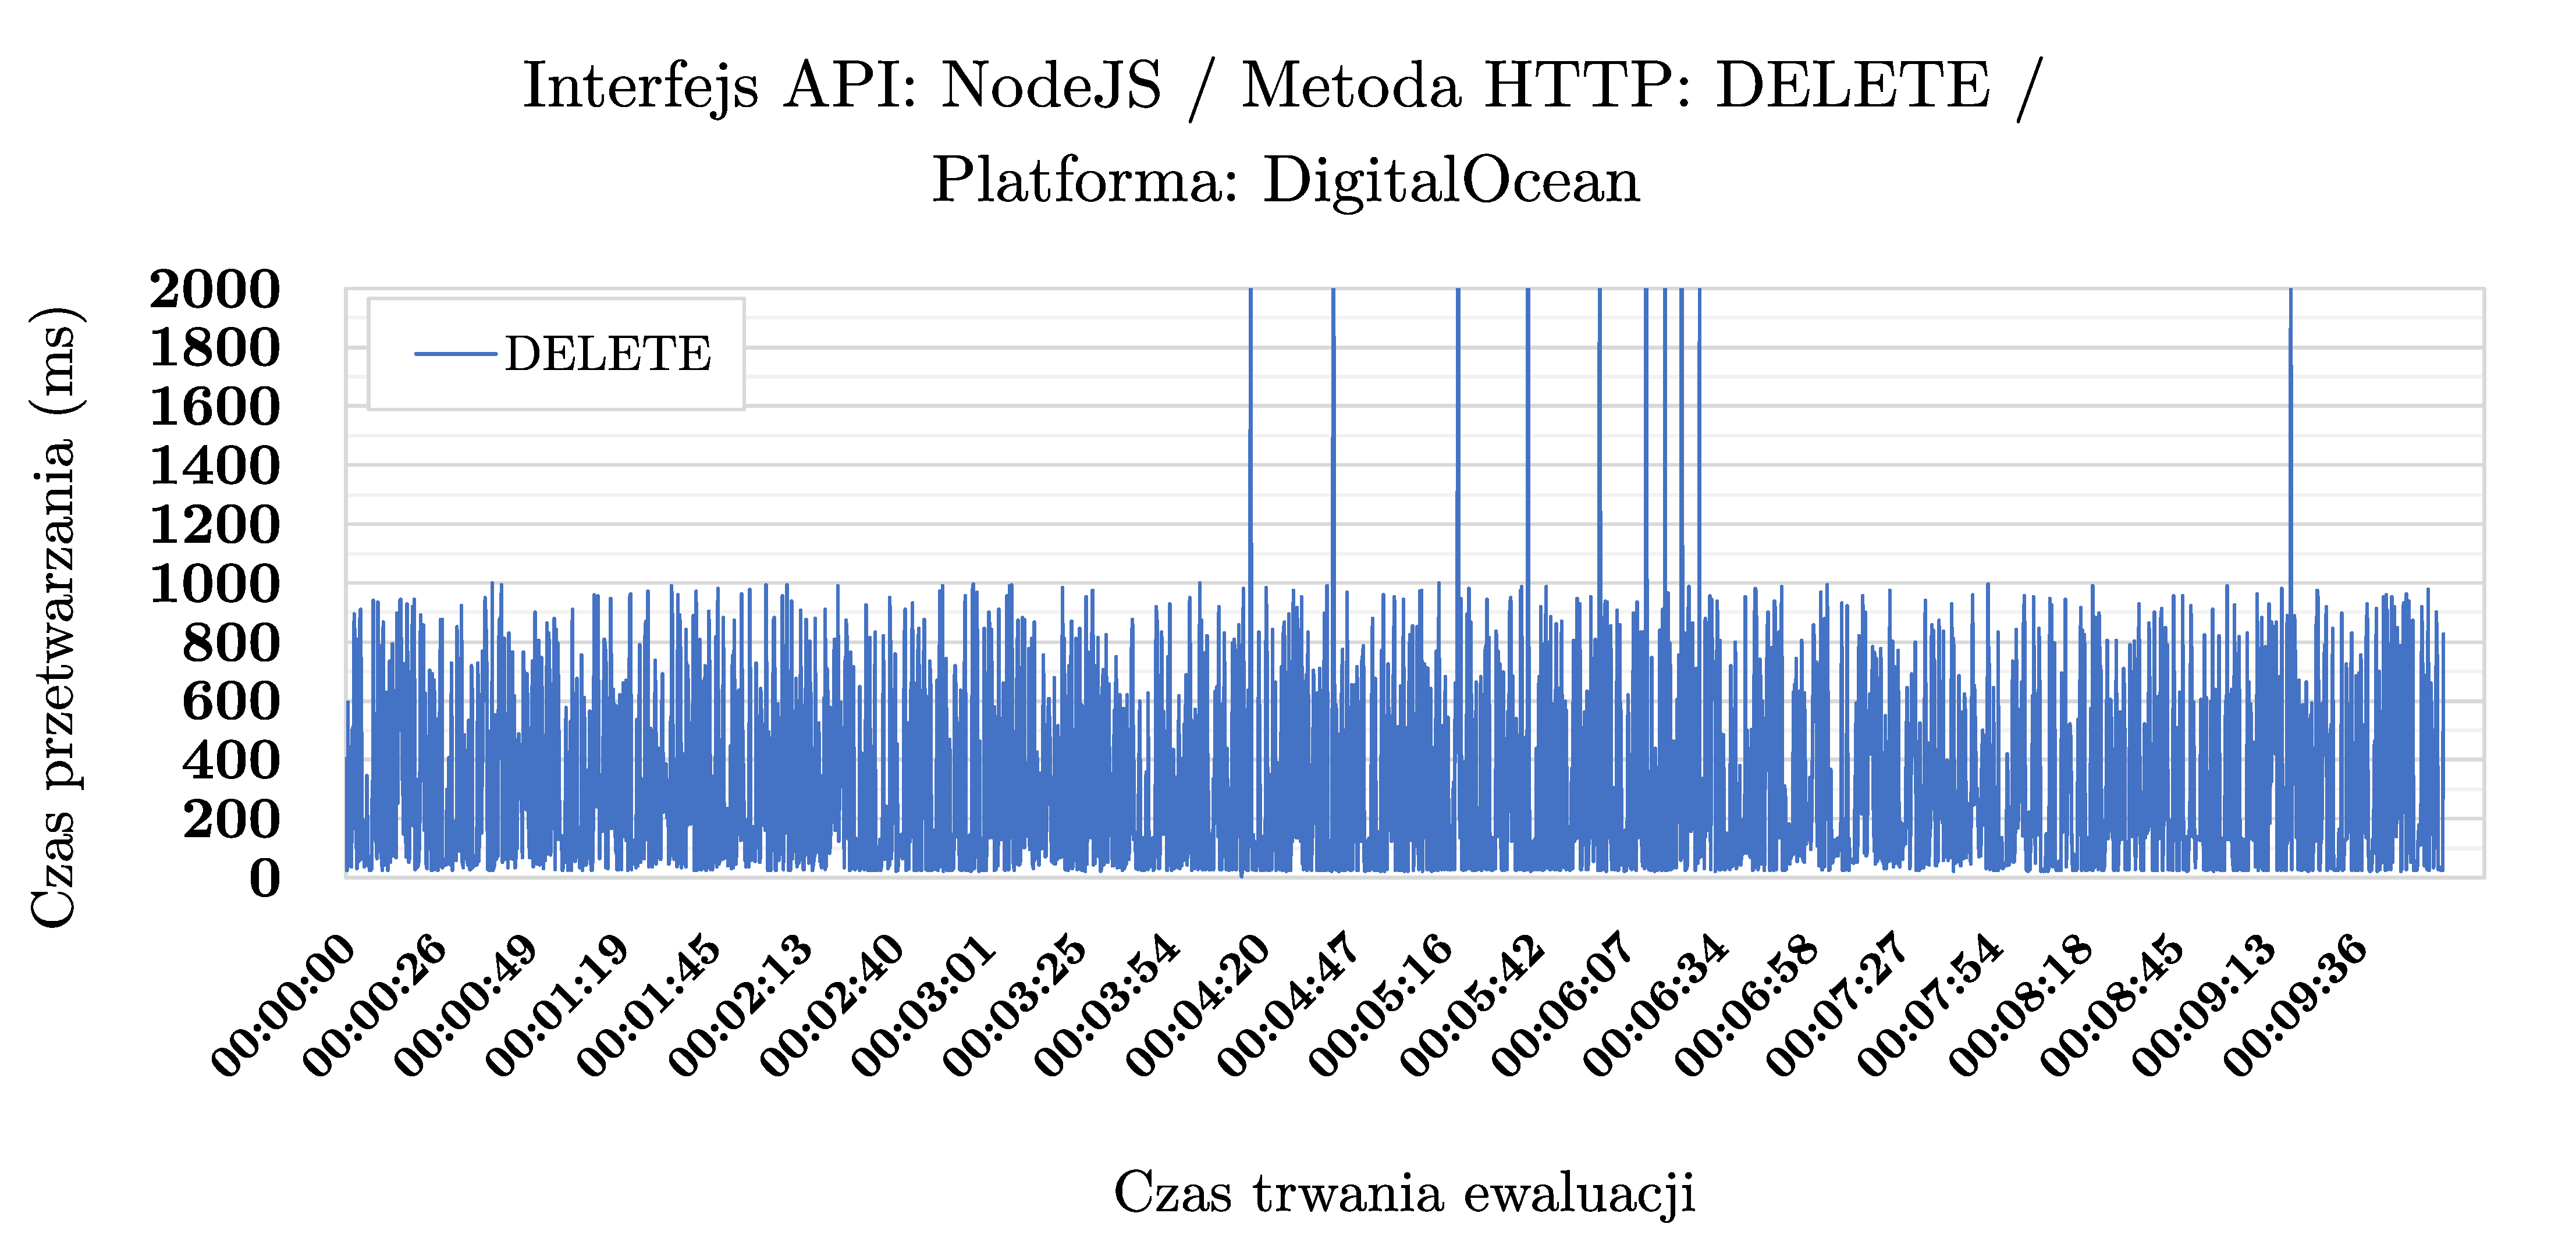
\includegraphics[width=0.49\textwidth]{rys05/nodejs-delete-digitalocean.pdf} \\
	% jezeli obraki sa rownej wysokosci, mozna je wyrownac do gory stosujac vtop jak nizej
	% \vtop{\vskip-2ex\hbox{{\includegraphics[width=0.475\textwidth]{rys05/beta1}}}} &
	% \vtop{\vskip-2ex\hbox{{\includegraphics[width=0.475\textwidth]{rys05/alfa1}}}}  \caption{Wyznaczanie trajektorii lotu rakiety: 
	\end{tabular}
  \caption{Wydajność działania mierzona czasem wewnętrznego przetwarzania operacji CRUD dla platform Heroku oraz DigitalOcean -- Interfejs API NodeJS}
  \label{fig:nodejs-heroku-vs-digitalocean}
\end{figure}

Kolejna z zaprezentowanych wizualizacji, dotyczy z kolei interfejsu API zaimplementowanego w oparciu o technologię NodeJS, który uruchomiony został na platformie Heroku (konfiguracja dedykowana), a także serwerze udostępnianym w ramach chmury DigitalOcean (konfiguracja generyczna). Zgromadzone czasy przetwarzania żądań dla odmiennych typów operacji pokazane zostały na wykresach \ref{fig:nodejs-heroku-vs-digitalocean} a) do \ref{fig:nodejs-heroku-vs-digitalocean} h).

Odnosząc się do analizowanej technologii, wzrost wydajności rozwiązania dedykowanego względem generycznego jest wydatny, i niezależnie od wybranego typu wykonywanej operacji, różnica wartości metryki go opisującaj jest niemniejsza niż 237 ms. Ponadto, w momencie w którym 99,98\% wszystkich obserwacji należy do przedziału od 34 ms do 900 ms w kontekście rozwiązania dedykowanego, tylko 72,7\% próbek badania dla rozwiązania generycznego, zawarte jest w analogicznym przedziale. Zauważyć należy fakt braku zwiększenia się intensywności żądań dla czasów przetwarzania powyżej 1000 ms, w odniesieniu do rozwiązania generycznego. Co prawda zapytania trwające powyżej 1000 ms pojawiają się w tego typu konfiguracji, to podobnie do rozwiązania dedykowanego, są to obserwacje jednostkowe.  

Kolejną metryką wziętą pod uwagę w ramach niniejszego badania jest liczba niepoprawnych odpowiedzi, które zostały zwrócone dla wygenerowanych zapytań. Podobnie jak dla wizualizacji zaprezentowanych powyżej, w tym przypadku, analiza również prowadzona będzie pod kątem obserwacji różnic wynikających z zastosowania odmiennych platform wdrożeniowych, a nie technologii implementacji interfejsów api. Na wykresach \ref{fig:errors-for-plaforms} a) oraz \ref{fig:errors-for-plaforms} b) przedstawiono wartości odnotowane względem omawianej metryki.

\begin{figure}[htb]
  \centering
	\begin{tabular}{@{}ll@{}}
    a) & b) \\
    \includegraphics[width=0.49\textwidth]{rys05/nodejs-errors.pdf} & \includegraphics[width=0.49\textwidth]{rys05/dotnet-errors.pdf} \\
	% jezeli obraki sa rownej wysokosci, mozna je wyrownac do gory stosujac vtop jak nizej
	% \vtop{\vskip-2ex\hbox{{\includegraphics[width=0.475\textwidth]{rys05/beta1}}}} &
	% \vtop{\vskip-2ex\hbox{{\includegraphics[width=0.475\textwidth]{rys05/alfa1}}}}  \caption{Wyznaczanie trajektorii lotu rakiety: 
	\end{tabular}
  \caption{Liczba błędnych odpowiedzi względem typu żądania oraz platformy wdrożeniowej}
  \label{fig:errors-for-plaforms}
\end{figure}


W przypadku interfejsu implementowanego z wykorzystaniem platformy NodeJS oraz języka JavaScript różnice wydajnościowe uwidaczniają się jeszcze bardziej w momencie w którym brana pod uwagę jest liczba niepowodzeń realizacji zapytań klienckich. Niezależnie od typu operacji, rozwiązanie wdrożone na platformie Heroku, generowało mniejszą liczbę błędnych odpowiedzi. Przytaczając najbardziej skrajny przypadek (tj. żądania typu GET), liczba niezrealizowanych poprawnie zapytań dla platformy generycznej jest ponad dwa razy większa, od tej dla platformy dedykowanej.

Analogiczną tendencję zaobserwować możemy w przypadku interfejsu programowania aplikacji C\# .NET. Tu również, niezależnie od metody protokołu hipertekstowego, rozwiązanie rekomendowane przez twórcę technologii posiada przewagę. Przewaga ta, najbardziej widoczna jest dla żądania typu PUT i wynosi ona 37 niepoprawnych odpowiedzi. Warto zaznaczyć, że całkowita liczba błędnie zrealizowanych żądań dla metody PUT oraz platformy dedykowanej wynosi 26.

Wyniki przeprowadzonego w tej sekcji badania posiadają najbardziej jednoznaczny charakter spośród wszystkich rezultatów otrzymanych w kontekście każdego z przeprowadzonych badań. Co więcej, rezultaty te, prowadzą do sformułowania popartego badaniami wniosku, że niezależnie od faktu, która z technologii implementacyjnych zostanie wybrana, a także jakiego typu operacje będą realizowane, system internetowy przygotowany do przejścia w fazę produkcyjną, powinien być wdrażany z wykorzystaniem narzędzi oraz infrastruktur dedykowanych względem określonej technologii. Usprawnienia wydajnościowe, wprowadzane przez twórców określonych środowisk chmurowych, pozwalają na korzystanie z usług sieciowych w sposób bardziej efektywny, a także generujący mniejszą liczbę błędów.